\documentclass{article} % For LaTeX2e
\usepackage{iclr2023_conference,times}
\iclrfinalcopy

% Optional math commands from https://github.com/goodfeli/dlbook_notation.
\input{math_commands.tex}

\usepackage{hyperref}
\usepackage{url}
\usepackage{subcaption}
\usepackage{adjustbox}
\usepackage{multirow}
\usepackage{makecell}
\usepackage{pgfplotstable}
\usepackage{booktabs}
\usepackage{xspace}
\usepackage{wrapfig}
\usepackage{cleveref}
\usepackage{colortbl}
\usepackage{bm}
\usepackage{tabularx}

\definecolor{mycolor}{RGB}{220,220,220}
\renewcommand\theadfont{}
% \usepackage{minipage}
% \pgfplotsset{compat=1.18}

% \title{AN EMPIRICAL ANALYSIS OF TECHNIQUES TO IMPROVE DETERMINISTIC UNCERTAINTY METHODS}
\title{Training, Architecture, and Prior \\for Deterministic Uncertainty Methods}

% Authors must not appear in the submitted version. They should be hidden
% as long as the \iclrfinalcopy macro remains commented out below.
% Non-anonymous submissions will be rejected without review.

\author{%
  Bertrand Charpentier, Chenxiang Zhang, Stephan Günnemann \\
  Technical University of Munich, Germany\\
  \texttt{\{charpent,zch,guennemann\}@in.tum.de} \\
}

% The \author macro works with any number of authors. There are two commands
% used to separate the names and addresses of multiple authors: \And and \AND.
%
% Using \And between authors leaves it to \LaTeX{} to determine where to break
% the lines. Using \AND forces a linebreak at that point. So, if \LaTeX{}
% puts 3 of 4 authors names on the first line, and the last on the second
% line, try using \AND instead of \And before the third author name.

\newcommand{\fix}{\marginpar{FIX}}
\newcommand{\new}{\marginpar{NEW}}

% \iclrfinalcopy % Uncomment for camera-ready version, but NOT for submission.
\begin{document} 


\maketitle

\begin{abstract}
Accurate and efficient uncertainty estimation is crucial to build reliable Machine Learning (ML) models capable to provide calibrated uncertainty estimates, generalize and detect Out-Of-Distribution (OOD) datasets. To this end, Deterministic Uncertainty Methods (DUMs) is a promising model family capable to perform uncertainty estimation in a single forward pass. This work investigates important design choices in DUMs: 
\textbf{(1)} we show that \emph{training} schemes decoupling the core architecture and the uncertainty head schemes can significantly improve uncertainty performances. 
\textbf{(2)} we demonstrate that the core \emph{architecture} expressiveness is crucial for uncertainty performance and that additional architecture constraints to avoid feature collapse can deteriorate the trade-off between OOD generalization and detection. 
\textbf{(3)} Contrary to other Bayesian models, we show that the \emph{prior} defined by DUMs do not have a strong effect on the final performances.
\end{abstract}

\section{Introduction}
%\label{sec:introduction_008}

% \looseness=-1
% Safety is critical to the adoption of deep learning in domains such as autonomous driving, medical diagnosis, or financial trading systems. A solution for this problem is to create reliable models capable to estimate the uncertainty of its own predictions. 
% Different uncertainty types are divided in \textit{aleatoric} uncertainty quantified by the inherited noise in the data, thus irreducible; \textit{epistemic} uncertainty quantified by the modeling choice or lack of data, thus reducible; \textit{predictive} uncertainty, a combination of aleatoric and epistemic \citep{gal2016uncertainty}. 
% In practice, high quality uncertainty estimates must be calibrated and able to detect Out-Of-Distribution (OOD) data like anomalies while preserving good Out-Of-Distribution (OOD) generalization performances like on dataset shifts.

While we have focused in the previous sections on proposing new Bayesian models for efficient uncertainty estimation on independent data, we now turn our attention on the practical considerations when using efficient uncertainty estimation methods. 

Recently, a family of methods for uncertainty estimation named Deterministic Uncertainty Methods (DUMs) have emerged \citep{postels2022practicalitydum}. 
Contrary to uncertainty methods such as Ensembles \citep{ensembles}, MC Dropout \citep{dropout} or other Bayesian neural networks on weights \citep{bayesian-networks}, which require multiple forward passes to make predictions, DUMs only require a single forward pass, thus making them significantly more computationally efficient. 
%These models can make predictions in only a single forward pass,  %thus being computationally efficient. 
Generally, DUMs are composed of three components with high potential impact on their performances: the \emph{training} procedure which is supposed to optimize the model toward high predictive and uncertainty performances,  the core \emph{architecture} which is supposed to define informative embeddings used to make predictions, and the \emph{prior} which is supposed to define the default uncertain predictions. In this work, we investigate the role of these three components on the quality of DUMs uncertainty estimates by evaluating calibration performances, OOD detection, and OOD generalization. Our main contributions are:
\vspace{-2mm}
\begin{itemize}
%\setlength\itemsep{-1mm}
    \item \textbf{Training}: We show that \emph{decoupling the learning rates} of the core architecture and uncertainty heads of DUMs, \emph{jointly training} the core architecture and the uncertainty head of DUMs, and \emph{pretraining} with \emph{more data} and \emph{higher data quality} improve uncertainty performances. 
    \item \textbf{Architecture}: We demonstrate that the expressiveness of the core architecture defined by the \emph{architecture type}, \emph{architecture size}, and \emph{dimension of the latent space} is crucial for \emph{both} predictive and uncertainty performances. Further, we show that applying additional regularization constraints to avoid \emph{feature collapse} does not find better trade-off between OOD detection and generalization, even sometimes degrading performances.
    \item \textbf{Prior}: In contrast to Bayesian neural networks on weights where the choice of prior is critical \citep{bayesposterior2020wenzel, fortuin2022prior, noci2021prior_cpe, kapoor2022prior_cpe}, we empirically show that the choice of prior defined in the training loss or in the uncertainty head of DUMs has a relatively small effect on the final uncertainty performances.
\end{itemize}

% \section{Related work}
\label{sec:related_work}

% add papers not related to this work
The existence of adversarial examples is a problematic property of neural networks \citep{szegedy2014, goodfellow2014}. Previous works have study this phenomena by proposing adversarial attacks \citep{carlini2016, brendel2018,DBLP:conf/kdd/ZugnerAG18}, defenses \citep{cisse2017, gu2015} and verification techniques  \citep{wong2017, singh2019krelu, cohen2019, DBLP:conf/icml/BojchevskiKG20, kopetzki2021}. This includes the study of different settings such as i.i.d. inputs, sequential inputs and graphs \citep{zheng2016, DBLP:conf/nips/BojchevskiG19, cheng2020, schuchardt2021}.

% related work
In the context of uncertainty estimation, robustness of the class prediction has been studied in previous works for Bayesian Neural Networks \citep{blundell2015, osawa2019, wesley2019}, drop out \citep{drop_out} or ensembles \citep{ensemble_simple} focusing on data set shifts \cite{snoek2019} or adversarial attacks \cite{robustness_bnn, cardelli2019, wicker2020}. Despite their efficient and high quality uncertainty estimates, the robustness of DBU models has not been investigated in detail yet --- indeed only for one single DBU model, \citep{malinin2019} has briefly performed attacks aiming to change the label. 
In contrast, our work focuses on a large variety of DBU models and analyzes two robustness properties: robustness of the class prediction w.r.t. adversarial perturbations and robustness of uncertainty estimation w.r.t.\ our newly proposed attacks against uncertainty measures. 


This so called \emph{uncertainty attack} directly targets uncertainty estimation and are different from traditional \emph{label attacks}, which target the class prediction \citep{madry2018, raphael2020}. They allow us to jointly evaluate robustness of the class prediction and robustness of uncertainty estimation. This goes beyond previous attack defenses that were either focused on evaluating \emph{robustness w.r.t.\ class predictions} \citep{carlini2016, clever_robustness} or detecting attacks against the class prediction \citep{bypassing_attack_detection}. 


Different models have been proposed to account for uncertainty while being robust.  \citep{smith2018} and \citep{simple_ood_adv_detection} have tried to improve label attack detection based on uncertainty using drop-out or density estimation. In addition to improving label attack detection for large unseen perturbations, \citep{stutz2020} aimed at improving robustness w.r.t. class label predictions on small input perturbations. They used adversarial training and soft labels for adversarial samples further from the original input. \citep{qin2020} suggested a similar adversarial training procedure, that softens labels depending on the input robustness. These previous works consider the aleatoric uncertainty that is contained in the predicted categorical probabilities, but in contrast to DBU models they are not capable of taking epistemic uncertainty into account. 



Recently, four studies tried to obtain certificates on aleatoric uncertainty estimates. \citep{single_model_quantile} and \citep{confidence_certificate_rs} compute confidence intervals and certificates on softmax predictions. \citep{bitterwolf2020} uses interval bound propagation to compute bounds on softmax predictions within the $L_{\infty}$-ball around an OOD sample using ReLU networks. \citep{meinke2020} focuses on obtaining certifiably low confidence for OOD data. These four studies estimate confidence based on softmax predictions, which accounts for aleatoric uncertainty only. In this paper, we provide certificates which apply for all uncertainty measures. In particular, we use our certificates on epistemic uncertainty measures such as differential entropy which are well suited for OOD detection.



% List of Papers on Robustness (group website)
%
%Anna-Kathrin Kopetzki, Stephan Günnemann
%Reachable sets of classifiers and regression models: (non-)robustness analysis and robust training
%Machine Learning Journal, 2021 --> cited
%
%Jan Schuchardt, Aleksandar Bojchevski, Johannes Klicpera, Stephan Günnemann
%Collective Robustness Certificates: Exploiting Interdependence in Graph Neural Networks
%International Conference on Learning Representations (ICLR), 2021
%
%Simon Geisler, Daniel Zügner, Stephan Günnemann
%Reliable Graph Neural Networks via Robust Aggregation
%Neural Information Processing Systems (NeurIPS), 2020
%
%Aleksandar Bojchevski, Johannes Klicpera, Stephan Günnemann
%Efficient Robustness Certificates for Discrete Data: Sparsity-Aware Randomized Smoothing for Graphs, Images and More
%International Conference on Machine Learning (ICML), 2020
%
%Daniel Zügner, Stephan Günnemann
%Certifiable Robustness of Graph Convolutional Networks under Structure Perturbations
%ACM SIGKDD Conference on Knowledge Discovery and Data Mining (KDD), 2020
%
%Daniel Zügner, Oliver Borchert, Amir Akbarnejad, Stephan Günnemann
%Adversarial Attacks on Graph Neural Networks: Perturbations and their Patterns
%ACM Transactions on Knowledge Discovery from Data, 2020
%
%Aleksandar Bojchevski, Stephan Günnemann
%Certifiable Robustness to Graph Perturbations
%Neural Information Processing Systems (NeurIPS), 2019
%
%Daniel Zügner, Stephan Günnemann
%Certifiable Robustness and Robust Training for Graph Convolutional Networks
%ACM SIGKDD Conference on Knowledge Discovery and Data Mining (KDD), 2019
%
%Aleksandar Bojchevski, Stephan Günnemann
%Adversarial Attacks on Node Embeddings via Graph Poisoning
%International Conference on Machine Learning (ICML), 2019
%
%Daniel Zügner, Stephan Günnemann
%Adversarial Attacks on Graph Neural Networks via Meta Learning
%International Conference on Learning Representations (ICLR), 2019
%
%Daniel Zügner, Amir Akbarnejad, Stephan Günnemann
%Adversarial Attacks on Neural Networks for Graph Data (Extended Abstract)
%International Joint Conference on Artificial Intelligence (IJCAI), 2019
%(Invited contribution to the IJCAI Sister Conference Best Paper Track)
%
%Daniel Zügner, Amir Akbarnejad, Stephan Günnemann
%Adversarial Attacks on Neural Networks for Graph Data 
%(Best Research Paper Award)
%ACM SIGKDD Conference on Knowledge Discovery and Data Mining (KDD), 2018
%
%
%Richard Leibrandt, Stephan Günnemann
%Making Kernel Density Estimation Robust towards Missing Values in Highly Incomplete Multivariate Data without Imputation
%SIAM International Conference on Data Mining (SDM), 2018 
%
%Aleksandar Bojchevski, Stephan Günnemann
%Bayesian Robust Attributed Graph Clustering: Joint Learning of Partial Anomalies and Group Structure
%AAAI Conference on Artificial Intelligence, pp. 2738-2745, 2018
%
%Aleksandar Bojchevski, Yves Matkovic, Stephan Günnemann
%Robust Spectral Clustering for Noisy Data: Modeling Sparse Corruptions Improves Latent Embeddings
%ACM SIGKDD Conference on Knowledge Discovery and Data Mining (KDD), pp. 737-746, 2017


\section{Deterministic Uncertainty Methods}
\label{sec:dum}

We consider a classification task where the goal is to predict the label $y\dataix \in \{ 1, \ldots , \nclass \}$ based on the input feature $\vx\dataix \in \real^{\inputdim}$. In this case, a DUM generally performs predictions in two main steps: \textbf{(1)} A core \emph{architecture} $f_\mathbf{\phi}$ maps the input features $\vx\dataix \in \real^{\inputdim}$ to a latent representation $\vz\dataix \in \real^{\latentdim}$, i.e. $f_\mathbf{\phi}(\vx\dataix)=\vz\dataix$. In practice, important design choices are the latent dimension $\latentdim$ and the architecture $f_\mathbf{\phi}$ which should be adapted to the task (see \cref{sec:architecture}). Further, multiple works proposed to apply additional bi-Lipschitz or reconstruction constraints to enrich the informativeness of the latent representation $\vz\dataix$ (see \cref{sec:architecture}). \textbf{(2)} An \emph{uncertainty head} $g_\mathbf{\psi}$ maps the latent representation $\vz\dataix$ to a predicted label $\hat{y}\dataix$ and an associated (aleatoric, epistemic, or predictive) uncertainty estimate $u\dataix$, i.e. $g_\mathbf{\psi}(\vz\dataix)=(\hat{y}\dataix, u\dataix)$. In practice, important design choices are the type of uncertainty head which are generally instantiated with a Gaussian Process (GP) \citep{uncertainty-distance-awareness, due, duq, uceloss, charpentier2022uncertainty-rl}, a density estimator \citep{charpentier2020, NatPN2021, charpentier2022uncertainty-rl, graph-postnet, uceloss, mukhoti2021ddu, postels2020mir, contrastive-ood, wu2020contrastive}, or an evidential model \citep{charpentier2020, NatPN2021, charpentier2022uncertainty-rl, graph-postnet, uceloss, malini2018}, and the choice of the prior used by the uncertainty head (see \cref{sec:prior}). Beyond core architecture and uncertainty head, another important choice is the training procedure which can either couple or decouple the parameters of the core architecture and uncertainty head (see \cref{sec:training}).

In this work we focus on two recent DUMs which cover different types of uncertainty heads: Natural Posterior Network (NatPN) \cite{NatPN2021} which learns an evidential distribution based on density estimation on the latent space, and Deterministic Uncertainty Estimator (DUE) \citep{due} which learns a deep Gaussian Process by parametrizing learnable inducing points in the latent space (see \cref{appendix:dums} for further method details). While NatPN is capable to differentiate aleatoric, epistemic, and predictive uncertainty, DUE only outputs the predictive uncertainty. 
For all the experiments, we use the same default setup: we first \emph{pretrain} the encoder with the cross-entropy loss until convergence, then load the pretrained encoder and jointly \emph{train} the encoder and uncertainty head (see \cref{subsec:appendix_training,subsec:appendix_encoder,subsec:appendix_prior} for further component details). We report the predictive performance via accuracy, and the uncertainty performances with Brier Score and OOD detection results after averaging over 5 seeds (see \cref{sec:metric_details} for further metric details). We perform our experiments on MNIST \citep{mnist}, CIFAR10 and CIFAR100 \citep{cifar10}, and Camelyon \citep{wilds}. OOD results reported in 
\cref{tab:training_schema,tab:training_pretrain,tab:encoder_architecture,tab:kernel} averages the uncertainty estimation from five OOD datasets: SVHN, STL10, CelebA, Camelyon and SVHN OODom \citep{svhn, coates2011stl10, celeba}. Our code and additional material is available online\footnote{\url{https://www.cs.cit.tum.de/daml/training-architecture-prior-dum/}}.

\textbf{Related work.} Previous works survey OOD detection methods \citep{ood-detection-survey}, OOD generazilation methods \citep{ood-generalization-survey}, or a wide range of uncertainty estimation methods \citep{uncertainty-survey,psaros2023uncertainty,survey_evidential_uncertainty,review-uncertainty-dl} by presenting key methods and challenges. These surveys do not focus on deterministic methods and do not make empirical analysis.
Other works propose great empirical studies to compare uncertainty estimation methods under shifts \citep{dataset-shift}, or analyze the role of the prior in Bayesian neural networks on weights \citep{bayesposterior2020wenzel, fortuin2022prior, noci2021prior_cpe, kapoor2022prior_cpe}. These works do not focus on DUMs. Closer to our work, \citet{postels2022practicalitydum} compares methods in the DUMs family and demonstrate calibration limitations. In contrast, we evaluate the role of \emph{components} in DUMs and show that carefully specifying \emph{training}, \emph{architecture}, or \emph{prior} can improve uncertainty metrics like calibration and OOD detection but also ID and OOD predictive performances.

% A detailed survey on uncertainty estimation was conducted by \cite{gawlikowski2021survey}, providing a taxonomy for supervised learning uncertainty estimation. A specific survey focusing on DUMs was done by \cite{postels2022practicalitydum}. By following its experimental settings, we evaluate the performance by considering both uncertainty estimation and the calibration on ID and OOD data. Further, we apply different regularization techniques to DUMs and analyze the results from uncertainty estimation and domain generalization evaluated on corrupted \citep{hendrycks2019corrupted} and in-the-wild distribution shifted datasets \citep{koh2021wilds}.
% \citet{minderer2021calibration}

\section{Training for DUMs}
\label{sec:training}

In this section, we study the importance of the training procedure in the performance of DUMs. To this end, we look at \emph{decoupling the learning rates} of the core encoder architecture and the uncertainty head, different \emph{training schemes}, and different \emph{pretraining schemes}.

\textbf{Decoupling learning rates.} We decouple the learning rates of the core architecture and the uncertainty head. We show the validation results for CIFAR100 as ID and SVHN as OOD with the core architecture ResNet18 in \cref{fig:decoupled_test}.
\underline{\textit{Observation:}} We observe that, when using different learning rates for the core architecture and the uncertainty head, NatPN improves Brier Score and OOD epistemic results and DUE significantly improves both predictive and uncertainty results. Hence, this shows that decoupling learning rates can improve results of DUMs, thus suggesting that the core architecture and the uncertainty head have training dynamics which requires different considerations.

\begin{figure}[!htb]
    \centering
    \includegraphics[width=0.8\linewidth]{sections/008_iclr2023/figures/decoupled_test.pdf}
    \caption{Results of DUMS on CIFAR100 with ResNet18 when \textbf{decoupling learning rates} of the core architecture and the uncertainty head. Decoupling learning rates improve DUMs performance. }
    \label{fig:decoupled_test}
\end{figure}

\textbf{Training schemes.} We compare two settings: the \textit{joint} training in which we jointly train the weights of the core architecture and uncertainty head, and the \textit{sequential} training in which we only train the uncertainty head by keeping the weights of the pretrained core architecture fixed. For each of the setting, we apply two additional techniques to stabilize the training: adding a \textit{batch normalization} to the last layer of the encoder to enforce latent representations to locate in a normalized region \citep{ioffe2015bn,NatPN2021}, and \textit{resetting the last layer} to retrain its weights to improve robustness to spurious correlation \citep{kirichenko2022reset}. We show the results for CIFAR100 as ID and five difference OOD datasets with the ResNet18 as core architecture in \cref{tab:training_schema} and additional results in the appendix \cref{tab:training_schema_ood}.
\underline{\textit{Observation:}} We observe that, compared to its sequential counterpart, joint training consistently improves DUMs performance for most metrics, thus suggesting that joint training should be preferred in practice for DUMs. Furthermore, while the GP-based method DUE does not benefit from stabilization techniques, we observe that they can significantly increase performance of the density-based method NatPN. This behavior is intuitively explained by the practical difficulty to accurately fit densities in high dimensional latent space. This can be significantly improved by using more powerful density estimator (see \cref{tab:normalizing_flow} in appendix).

\textbf{Pretraining schemes.} We compare multiple training schemes which differ in terms of \emph{amount} and \emph{quality} of data used for pretraining. Hence, we do not pretrain the core architecture or pretrain it with 10\% of CIFAR100, 100\% of CIFAR100 without and with Gaussian noise, or ImageNet. We show the results for CIFAR100 as ID and five different OOD datasets with ResNet50 as core architecture in \cref{tab:training_pretrain} and additional results in the appendix \cref{tab:training_pretrain_ood}.
\underline{\textit{Observation:}} We observe that, while too few data for pretraining does not improve final performance of DUMs, the overall performance significantly increase when the encoder is pretrained with high quantity and high quality of data.  Similarly to \citet{why-nf-fail-ood}, this suggests that the embedding quality is important to improve uncertainty quantification. Here, we show additionally that embeddings pretrained with many high quality data are crucial to facilitate the prediction of the uncertainty head.

\begin{table}[!htp]\centering
    \caption{Results of DUMs on CIFAR100 with ResNet18 under different \textbf{training schemes} using \textit{joint/sequential} training with no additional layer, an additional batch norm layer, or resetting the last layer. Gray cells indicate the best between \textit{joint/sequential} while bold numbers indicate the best overall. OOD results are averaged over OOD datasets. We observe that joint training works best and stabilization techniques can improve performances.}
    \label{tab:training_schema}
    \tiny
    
    \resizebox{0.9\textwidth}{!}{%
    \begin{tabular}{llccccc}
        \toprule
        \textbf{Method} &\textbf{Train Schema} &\textbf{Accuracy ($\uparrow$)} &\textbf{Brier Score ($\downarrow$)} &\textbf{OOD Pred. ($\uparrow$)} &\textbf{OOD Epis. ($\uparrow$)} \\
        \midrule
        \multirow{6}{*}{NatPN} 
        & joint &71.12 $\pm$ 0.18 & \cellcolor{mycolor}41.06 $\pm$ 0.18 & \cellcolor{mycolor}75.17 $\pm$ 1.60 & \cellcolor{mycolor}63.94 $\pm$ 2.80 \\
        & joint + bn &71.60 $\pm$ 0.14 &\cellcolor{mycolor}41.11 $\pm$ 0.12 & 74.22 $\pm$ 0.94 & \cellcolor{mycolor}66.17 $\pm$ 2.55 \\
        & joint + reset &71.61 $\pm$ 0.18 & \cellcolor{mycolor}\textbf{40.76 $\pm$ 0.18} &\cellcolor{mycolor}\textbf{75.35 $\pm$ 0.71} & \cellcolor{mycolor}\textbf{69.02 $\pm$ 1.49} \\
        % \cmidrule[0.1pt](lr){2-6}
        & sequential & \cellcolor{mycolor}\textbf{72.00 $\pm$ 0.19} &42.20 $\pm$ 0.09 &75.09 $\pm$ 0.86 &53.49 $\pm$ 2.56 \\
        & sequential + bn & \cellcolor{mycolor}71.98 $\pm$ 0.18 & 42.39 $\pm$ 0.11 & \cellcolor{mycolor}75.01 $\pm$ 0.86 &52.34 $\pm$ 2.81 \\
        & sequential + reset & \cellcolor{mycolor}71.79 $\pm$ 0.17 &40.95 $\pm$ 0.14 &74.63 $\pm$ 0.85 &61.90 $\pm$ 2.14 \\
        \midrule
        \multirow{6}{*}{DUE} 
        & joint & \cellcolor{mycolor}\textbf{72.33 $\pm$ 0.11} & \cellcolor{mycolor}\textbf{40.80 $\pm$ 0.11} &74.74 $\pm$ 0.89 &- \\
        & joint + bn & \cellcolor{mycolor}72.30 $\pm$ 0.09 & \cellcolor{mycolor}40.85 $\pm$ 0.12 &74.63 $\pm$ 0.95 &- \\
        & joint + reset & \cellcolor{mycolor}71.94 $\pm$ 0.12 & \cellcolor{mycolor}41.43 $\pm$ 0.12 &74.89 $\pm$ 0.76 &- \\
        % \cmidrule[0.1pt](lr){2-6}
        & sequential &72.07 $\pm$ 0.10 &41.66 $\pm$ 0.10 & \cellcolor{mycolor}74.82 $\pm$ 0.90 &- \\
        & sequential + bn &72.04 $\pm$ 0.13 &41.73 $\pm$ 0.11 & \cellcolor{mycolor}74.88 $\pm$ 0.95 &- \\
        & sequential + reset &71.56 $\pm$ 0.14 &42.30 $\pm$ 0.11 & \cellcolor{mycolor}\textbf{75.08 $\pm$ 1.01} &- \\
        \bottomrule
    \end{tabular}
    }
\end{table}

\begin{table}[!htp]\centering
    \caption{Results of DUMs with ResNet50 under different \textbf{pretraining schemes} using no pretraining, pretraining on 10\% of CIFAR100, 100\% of CIFAR100 without Gaussian noise and with Gaussian noise, or ImageNet. OOD results are averaged over OOD datasets. Bold numbers indicate best results among all settings. We observe that high quantity and high quality of data can improve performances.}
    \label{tab:training_pretrain}
    \tiny
    
    \resizebox{0.9\textwidth}{!}{%
    \begin{tabular}{llccccc}\toprule
        \textbf{Method} &\textbf{Pretrain Schema} &\textbf{Accuracy ($\uparrow$)} &\textbf{Brier Score ($\downarrow$)} &\textbf{OOD Pred. ($\uparrow$)} &\textbf{OOD Epis. ($\uparrow$)} \\
        \midrule
        \multirow{6}{*}{NatPN} &None &78.45 $\pm$ 1.94 &30.16 $\pm$ 2.57 &79.85 $\pm$ 3.30 &85.81 $\pm$ 2.05 \\
        &C100 (10\%) &67.25 $\pm$ 0.71 &44.69 $\pm$ 0.94 &68.10 $\pm$ 1.90 &78.50 $\pm$ 3.27 \\
        &C100 (100\%) + $\gN(0.5)$ &72.50 $\pm$ 1.07 &39.36 $\pm$ 1.43 &68.66 $\pm$ 3.76 &73.54 $\pm$ 1.84 \\
        &C100 (100\%) + $\gN(0.1)$ &75.25 $\pm$ 0.61 &35.99 $\pm$ 0.88 &69.78 $\pm$ 4.65 &75.81 $\pm$ 2.85 \\
        &C100 (100\%) &76.31 $\pm$ 0.45 &34.32 $\pm$ 0.51 &78.95 $\pm$ 3.19 &76.91 $\pm$ 2.64 \\
        &ImageNet &\textbf{84.22 $\pm$ 0.12} &\textbf{23.67 $\pm$ 0.27} &\textbf{84.95 $\pm$ 1.48} &\textbf{89.08 $\pm$ 0.70} \\
        \midrule
        \multirow{6}{*}{DUE} &None &72.41 $\pm$ 0.24 &47.35 $\pm$ 0.25 &80.04 $\pm$ 1.28 &- \\
        &C100 (10\%) &63.86 $\pm$ 0.58 &50.94 $\pm$ 0.53 &72.44 $\pm$ 1.32 &- \\
        &C100 (100\%) &76.38 $\pm$ 0.35 &36.89 $\pm$ 0.50 &81.71 $\pm$ 1.87 &- \\
        &C100 (100\%) + $\gN(0.5)$ &72.10 $\pm$ 1.00 &42.48 $\pm$ 1.18 &74.89 $\pm$ 1.97 &- \\
        &C100 (100\%) + $\gN(0.1)$ &75.31 $\pm$ 0.91 &38.31 $\pm$ 1.22 &79.43 $\pm$ 1.93 &- \\
        &ImageNet &\textbf{82.42 $\pm$ 0.14} &\textbf{28.09 $\pm$ 0.19} &\textbf{90.24 $\pm$ 0.51} &- \\
        \bottomrule
        \end{tabular}
    }
\end{table}






% \begin{table}[!htb]
% \centering
% \tiny

% \begin{minipage}[t]{0.48\textwidth}
% \caption{Results of DUMs on CIFAR100 with ResNet18 under different \textbf{training schemes} using \textit{joint/sequential} training with no additional layer, an additional batch norm layer, or resetting the last layer. Gray cells indicate the best between \textit{joint/sequential} while bold numbers indicate the best overall. OOD results are averaged over OOD datasets. We observe that joint training works best and stabilization techniques can improve performances.}
% \label{tab:training_schema}
% \resizebox{\textwidth}{!}{%
% \begin{tabular}{llccccc}
% \toprule
% \textbf{Method} &\textbf{Train Schema} &\textbf{Accuracy ($\uparrow$)} &\textbf{Brier Score ($\downarrow$)} &\textbf{OOD Pred. ($\uparrow$)} &\textbf{OOD Epis. ($\uparrow$)} \\
% \midrule
% \multirow{6}{*}{NatPN} 
% & joint &71.12 $\pm$ 0.18 & \cellcolor{mycolor}41.06 $\pm$ 0.18 & \cellcolor{mycolor}75.17 $\pm$ 1.60 & \cellcolor{mycolor}63.94 $\pm$ 2.80 \\
% & joint + bn &71.60 $\pm$ 0.14 &\cellcolor{mycolor}41.11 $\pm$ 0.12 & 74.22 $\pm$ 0.94 & \cellcolor{mycolor}66.17 $\pm$ 2.55 \\
% & joint + reset &71.61 $\pm$ 0.18 & \cellcolor{mycolor}\textbf{40.76 $\pm$ 0.18} &\cellcolor{mycolor}\textbf{75.35 $\pm$ 0.71} & \cellcolor{mycolor}\textbf{69.02 $\pm$ 1.49} \\
% % \cmidrule[0.1pt](lr){2-6}
% & sequential & \cellcolor{mycolor}\textbf{72.00 $\pm$ 0.19} &42.20 $\pm$ 0.09 &75.09 $\pm$ 0.86 &53.49 $\pm$ 2.56 \\
% & sequential + bn & \cellcolor{mycolor}71.98 $\pm$ 0.18 & 42.39 $\pm$ 0.11 & \cellcolor{mycolor}75.01 $\pm$ 0.86 &52.34 $\pm$ 2.81 \\
% & sequential + reset & \cellcolor{mycolor}71.79 $\pm$ 0.17 &40.95 $\pm$ 0.14 &74.63 $\pm$ 0.85 &61.90 $\pm$ 2.14 \\
% \midrule
% \multirow{6}{*}{DUE} 
% & joint & \cellcolor{mycolor}\textbf{72.33 $\pm$ 0.11} & \cellcolor{mycolor}\textbf{40.80 $\pm$ 0.11} &74.74 $\pm$ 0.89 &- \\
% & joint + bn & \cellcolor{mycolor}72.30 $\pm$ 0.09 & \cellcolor{mycolor}40.85 $\pm$ 0.12 &74.63 $\pm$ 0.95 &- \\
% & joint + reset & \cellcolor{mycolor}71.94 $\pm$ 0.12 & \cellcolor{mycolor}41.43 $\pm$ 0.12 &74.89 $\pm$ 0.76 &- \\
% % \cmidrule[0.1pt](lr){2-6}
% & sequential &72.07 $\pm$ 0.10 &41.66 $\pm$ 0.10 & \cellcolor{mycolor}74.82 $\pm$ 0.90 &- \\
% & sequential + bn &72.04 $\pm$ 0.13 &41.73 $\pm$ 0.11 & \cellcolor{mycolor}74.88 $\pm$ 0.95 &- \\
% & sequential + reset &71.56 $\pm$ 0.14 &42.30 $\pm$ 0.11 & \cellcolor{mycolor}\textbf{75.08 $\pm$ 1.01} &- \\
% \bottomrule
% \end{tabular}
% }\end{minipage}\quad%
% %
% %
% \begin{minipage}[t]{0.48\textwidth}
% \caption{Results of DUMs with ResNet50 under different \textbf{pretraining schemes} using no pretraining, pretraining on 10\% of CIFAR100, 100\% of CIFAR100 without Gaussian noise and with Gaussian noise, or ImageNet. OOD results are averaged over OOD datasets. Bold numbers indicate best results among all settings. We observe that high quantity and high quality of data can improve performances.}
% \label{tab:training_pretrain}

% \resizebox{\textwidth}{!}{%
% \begin{tabular}{llccccc}\toprule
% \textbf{Method} &\textbf{Pretrain Schema} &\textbf{Accuracy ($\uparrow$)} &\textbf{Brier Score ($\downarrow$)} &\textbf{OOD Pred. ($\uparrow$)} &\textbf{OOD Epis. ($\uparrow$)} \\
% \midrule
% \multirow{6}{*}{NatPN} &None &78.45 $\pm$ 1.94 &30.16 $\pm$ 2.57 &79.85 $\pm$ 3.30 &85.81 $\pm$ 2.05 \\
% &C100 (10\%) &67.25 $\pm$ 0.71 &44.69 $\pm$ 0.94 &68.10 $\pm$ 1.90 &78.50 $\pm$ 3.27 \\
% &C100 (100\%) + $\gN(0.5)$ &72.50 $\pm$ 1.07 &39.36 $\pm$ 1.43 &68.66 $\pm$ 3.76 &73.54 $\pm$ 1.84 \\
% &C100 (100\%) + $\gN(0.1)$ &75.25 $\pm$ 0.61 &35.99 $\pm$ 0.88 &69.78 $\pm$ 4.65 &75.81 $\pm$ 2.85 \\
% &C100 (100\%) &76.31 $\pm$ 0.45 &34.32 $\pm$ 0.51 &78.95 $\pm$ 3.19 &76.91 $\pm$ 2.64 \\
% &ImageNet &\textbf{84.22 $\pm$ 0.12} &\textbf{23.67 $\pm$ 0.27} &\textbf{84.95 $\pm$ 1.48} &\textbf{89.08 $\pm$ 0.70} \\
% \midrule
% \multirow{6}{*}{DUE} &None &72.41 $\pm$ 0.24 &47.35 $\pm$ 0.25 &80.04 $\pm$ 1.28 &- \\
% &C100 (10\%) &63.86 $\pm$ 0.58 &50.94 $\pm$ 0.53 &72.44 $\pm$ 1.32 &- \\
% &C100 (100\%) &76.38 $\pm$ 0.35 &36.89 $\pm$ 0.50 &81.71 $\pm$ 1.87 &- \\
% &C100 (100\%) + $\gN(0.5)$ &72.10 $\pm$ 1.00 &42.48 $\pm$ 1.18 &74.89 $\pm$ 1.97 &- \\
% &C100 (100\%) + $\gN(0.1)$ &75.31 $\pm$ 0.91 &38.31 $\pm$ 1.22 &79.43 $\pm$ 1.93 &- \\
% &ImageNet &\textbf{82.42 $\pm$ 0.14} &\textbf{28.09 $\pm$ 0.19} &\textbf{90.24 $\pm$ 0.51} &- \\
% \bottomrule
% \end{tabular}
% }\end{minipage}
% \end{table}

% \begin{table}[!htp]\centering
% \caption{\textbf{Pretrain schema.} Both DUMs benefits from the quantity of data under the ImageNet pretrained encoder. The reported OOD results are an average over all the independent OOD dataset result. The encoder ResNet50 from torchvision is used for the schemas.}
% \label{tab:training_pretrain}
% \tiny
% \begin{tabular}{llccccc}\toprule
% \textbf{Model} &\textbf{Pretrain Schema} &\textbf{Accuracy} &\textbf{Brier Score} &\textbf{OOD Pred.} &\textbf{OOD Epis.} \\
% \midrule
% \multirow{4}{*}{NatPN} &None &78.45 $\pm$ 1.94 &30.16 $\pm$ 2.57 &79.85 $\pm$ 3.30 &85.81 $\pm$ 2.05 \\
% &C100 (10\%) &67.25 $\pm$ 0.71 &44.69 $\pm$ 0.94 &68.10 $\pm$ 1.90 &78.50 $\pm$ 3.27 \\
% &C100 (100\%) &76.31 $\pm$ 0.45 &34.32 $\pm$ 0.51 &78.95 $\pm$ 3.19 &76.91 $\pm$ 2.64 \\
% &\textbf{ImageNet} &\textbf{84.22 $\pm$ 0.12} &\textbf{23.67 $\pm$ 0.27} &\textbf{84.95 $\pm$ 1.48} &\textbf{89.08 $\pm$ 0.70} \\
% \midrule
% \multirow{4}{*}{DUE} &None &72.41 $\pm$ 0.24 &47.35 $\pm$ 0.25 &80.04 $\pm$ 1.28 &- \\
% &C100 (10\%) &63.86 $\pm$ 0.58 &50.94 $\pm$ 0.53 &72.44 $\pm$ 1.32 &- \\
% &C100 (100\%) &76.38 $\pm$ 0.35 &36.89 $\pm$ 0.50 &81.71 $\pm$ 1.87 &- \\
% &\textbf{ImageNet} &\textbf{82.42 $\pm$ 0.14} &\textbf{28.09 $\pm$ 0.19} &\textbf{90.24 $\pm$ 0.51} &- \\
% \bottomrule
% \end{tabular}
% \end{table}

\section{Architecture for DUMs Details}
\label{subsec:appendix_encoder}


% -------------------------------------------


% \subsection{Regularization constraints}

For all the architecture experiments we used the default training settings in \cref{subsec:appendix_training} and \cref{tab:appendix_default_hyper}.

\textbf{Bi-Lipschitz training details.} In the \textit{None} configuration, we removed the residual connection from the architecture for both the pretraining of the encoder and the joint training phase. In the \textit{Residual} configuration, we did not modify anything since both ResNet and WideResNet already use the residual connection. While for the \textit{bi-Lipschitz} configuration, we added the spectral normalization during both the pretraining and also joint training phase. Following the original method presented in \cite{due}, we used the same implementation and applied spectral normalization to the linear, convolution, and batch normalization layers. During the model selection, using the validation set results, we find that the best \textit{Lipschitz constant} $c$ for DUE is 4, and for NatPN is 5. For both the models the power iteration parameter is set to 1. For the toy dataset we use an encoder with 4 linear layers of 128 dimension each.

\begin{figure}[!htb]
    \centering
    \includegraphics[width=\textwidth]{sections/008_iclr2023/figures/bi_bar.pdf}
    \caption{Results OOD generalization and OOD detection results of DUMs with none, residual and bi-lipschitz \textbf{architecture constraints}. Bi-lipschitz and more specifically can improve OOD detection by mitigating feature collapse (see \cref{fig:bi_toy}) at the expense of degrading OOD generalization.}
    \label{fig:bi_bar_full}
\end{figure}

\begin{figure}[!htb]
    \centering
    \includegraphics[width=0.75\textwidth]{sections/008_iclr2023/figures/reconst.pdf}
    \caption{Results OOD generalization and OOD detection results of DUMs with reconstruction \textbf{architecture constraints}. Increasing the strength of the reconstruction factor $\lambda$ improves the OOD generalization only on the simpler MNIST/CMNIST datasets but fails for more complex datasets. }
    \label{fig:reconst_full}
\end{figure}

\textbf{Reconstruction training details.} The decoder reconstructs the input extracted from the last residual block of the encoder, before the pooling layer. During the pretraining phase, both the encoder and decoder are trained with the cross-entropy loss plus a MSE reconstruction term. During the joint training phase, we load the pretrained encoder and decoder, and joint train with the DUMs' respective loss plus the MSE reconstruction term. For the toy dataset we use an encoder with 4 linear layers of 128 dimension each.

\begin{figure}[!htb]
    \begin{subfigure}[b]{\textwidth}
        \centering
        \includegraphics[width=0.75\textwidth]{sections/008_iclr2023/figures/toy/blob2/bi.png}
        \caption{Bi-Lipschitz}
        \label{fig:bi_toy}
    \end{subfigure}
    \begin{subfigure}[b]{\textwidth}
        \centering
        \includegraphics[width=0.75\textwidth]{sections/008_iclr2023/figures/toy/blob2/rec.png}
        \caption{Reconstruction}
        \label{fig:rec_toy}
    \end{subfigure}
    \caption{\textbf{Regularization constraint toy dataset uncertainty boundaries with NatPN.} The two black dots represent the center of two different class of Gaussian data, sharing the same y-axis to trigger the \textit{feature collapse} phenomenon. The color represents the likelihood produced by the uncertainty head. Each row is a different setting, e.g. \textit{bi1.0} is the bi-Lipschitz constraint with the Lipschitz constant $c = 1$ and \textit{rec1.0} is the reconstruction term with $\lambda=1$. Each column is a different seed initialization. (top) \textbf{Bi-Lipschitz} experiment shows that the core encoder architecture constrained with a larger \textit{Lipschitz constant} in the last two rows behaves similar to the encoder constrained with only the residual connection (second row) showing that relaxing the spectral normalization constraint falls back to the residual connection, preventing the feature collapse. (bottom) \textbf{Reconstruction} experiment shows that it does not help to prevent feature collapse by itself. The core encoder architecture is not constrained with bi-Lipschitz. }
    \label{fig:toy}
\end{figure}

\begin{figure}[!htb]
    \begin{subfigure}[b]{\textwidth}
        \centering
        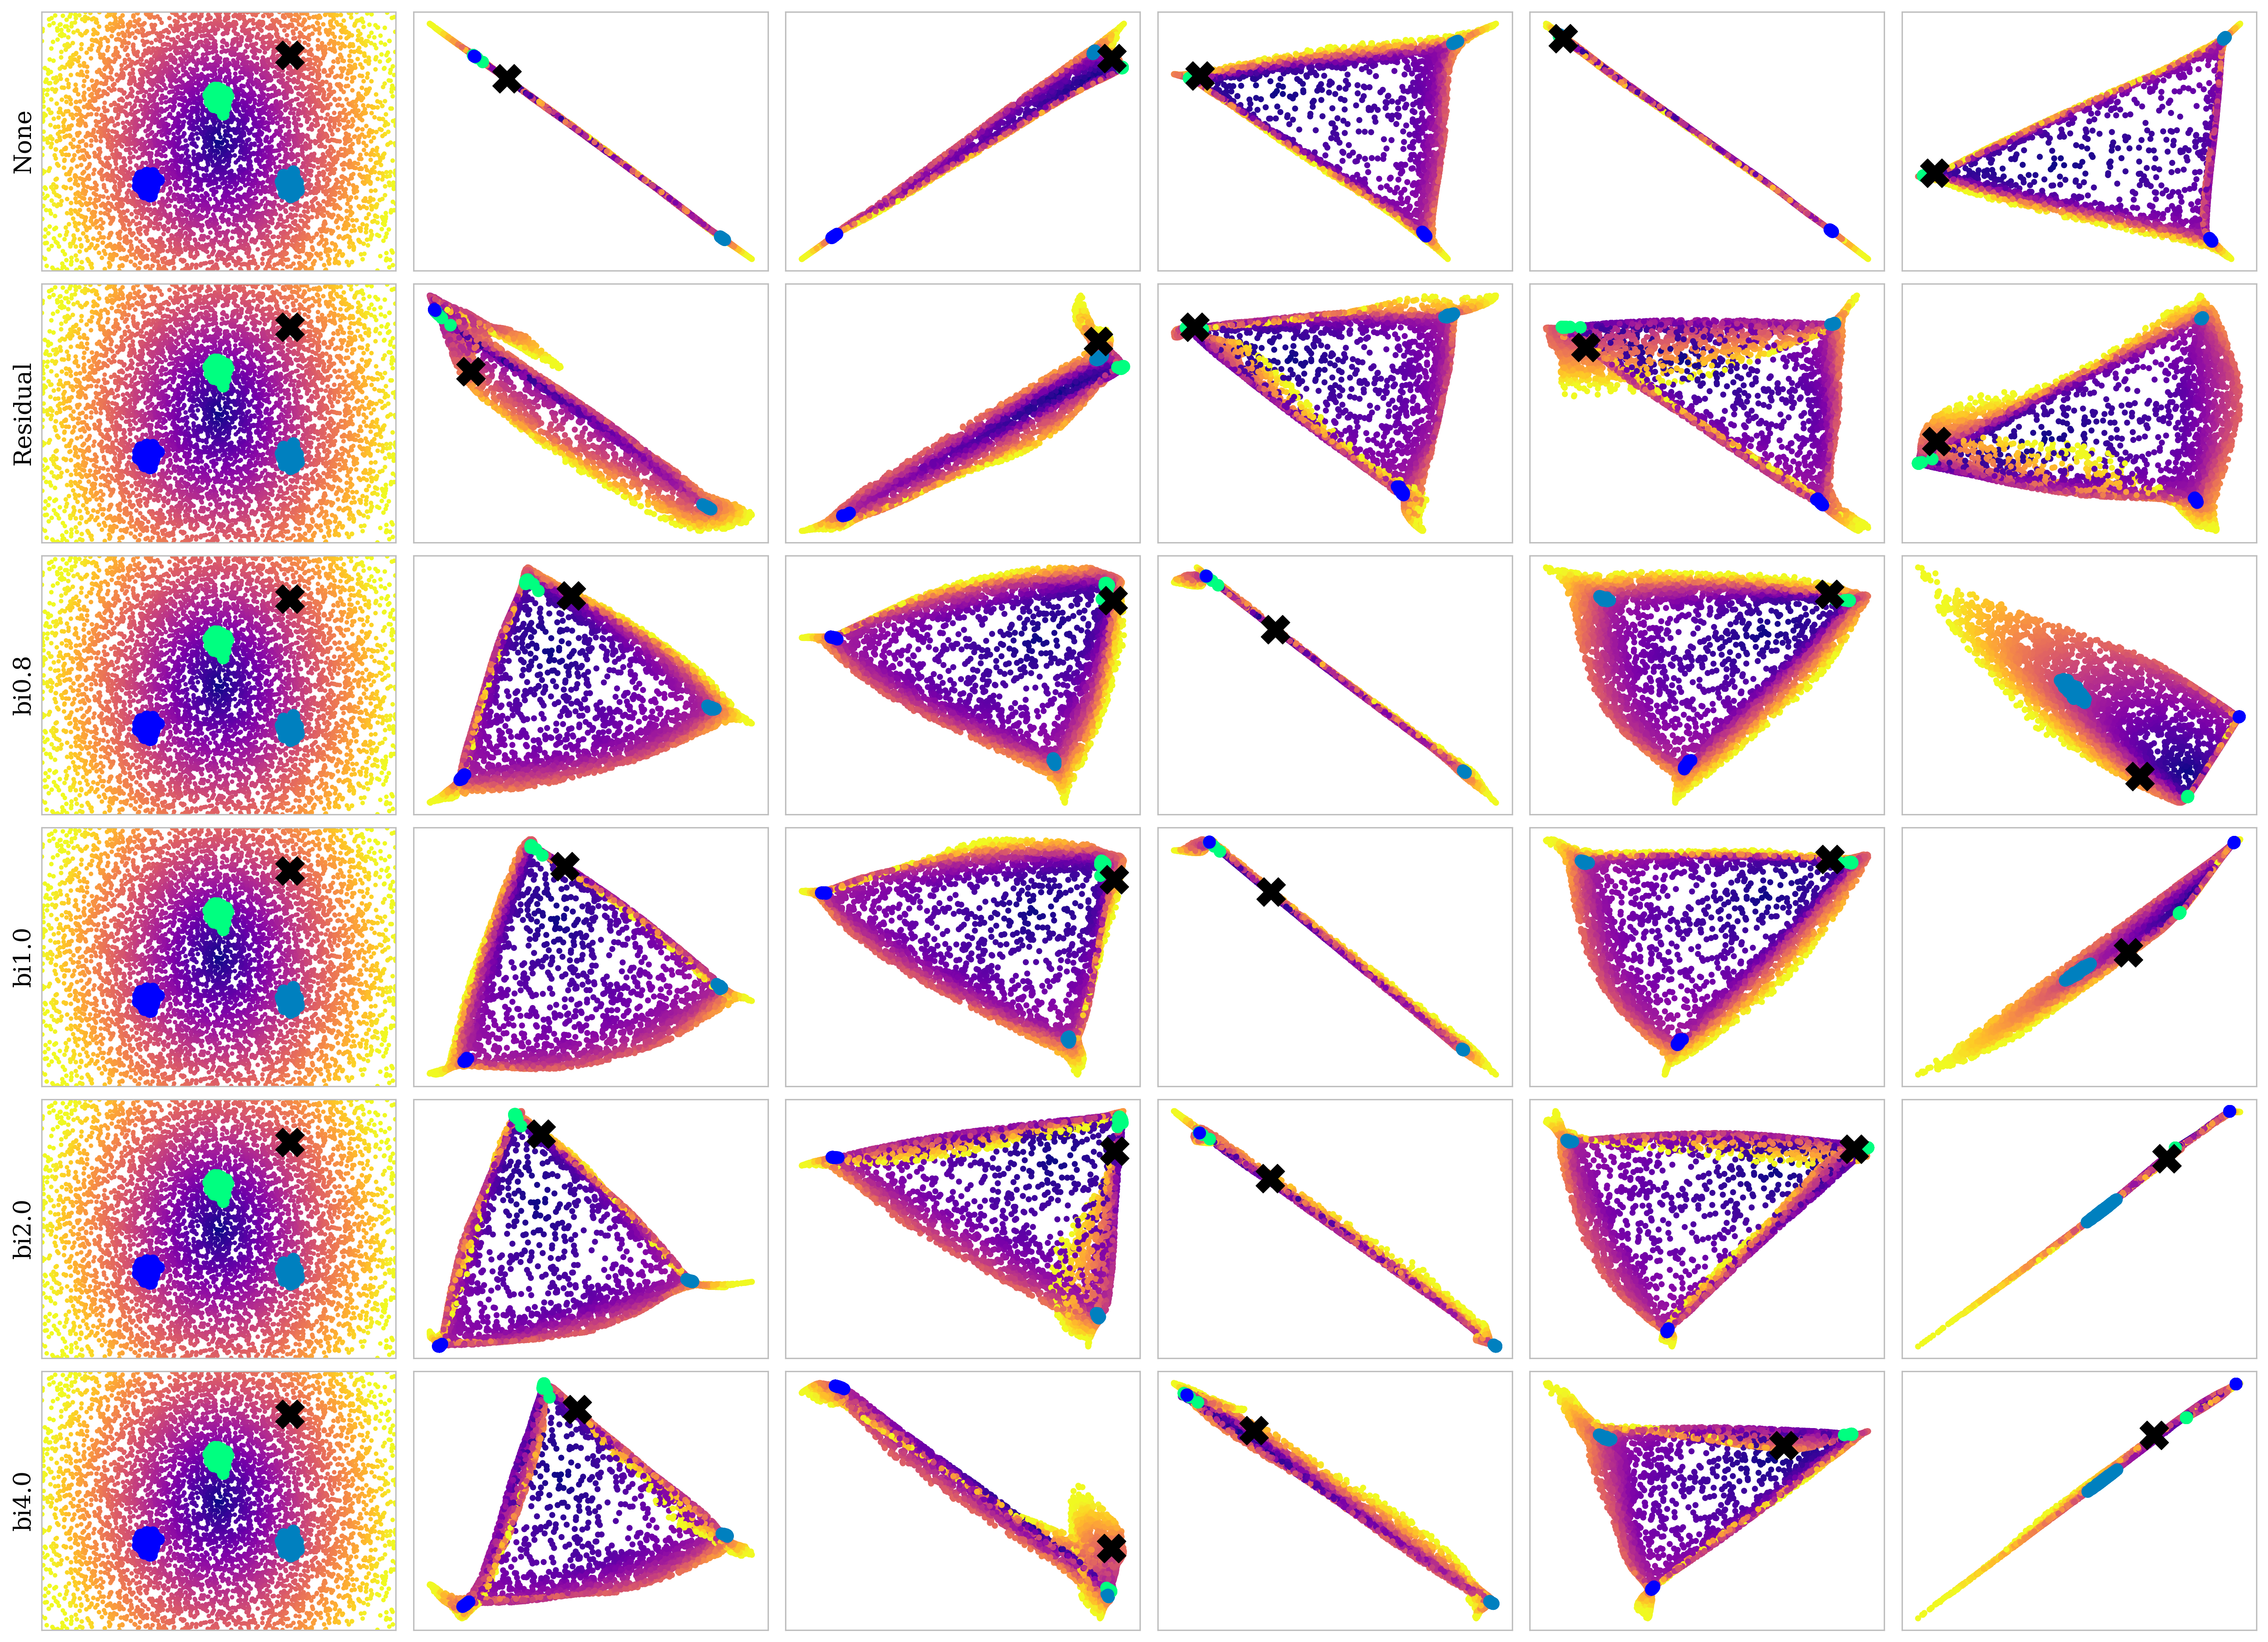
\includegraphics[width=0.8\textwidth]{sections/008_iclr2023/figures/toy/blob2/bi_collapse.png}
        \caption{Bi-Lipschitz}
        \label{fig:bi_toy_collapse}
    \end{subfigure}
    \begin{subfigure}[b]{\textwidth}
        \centering
        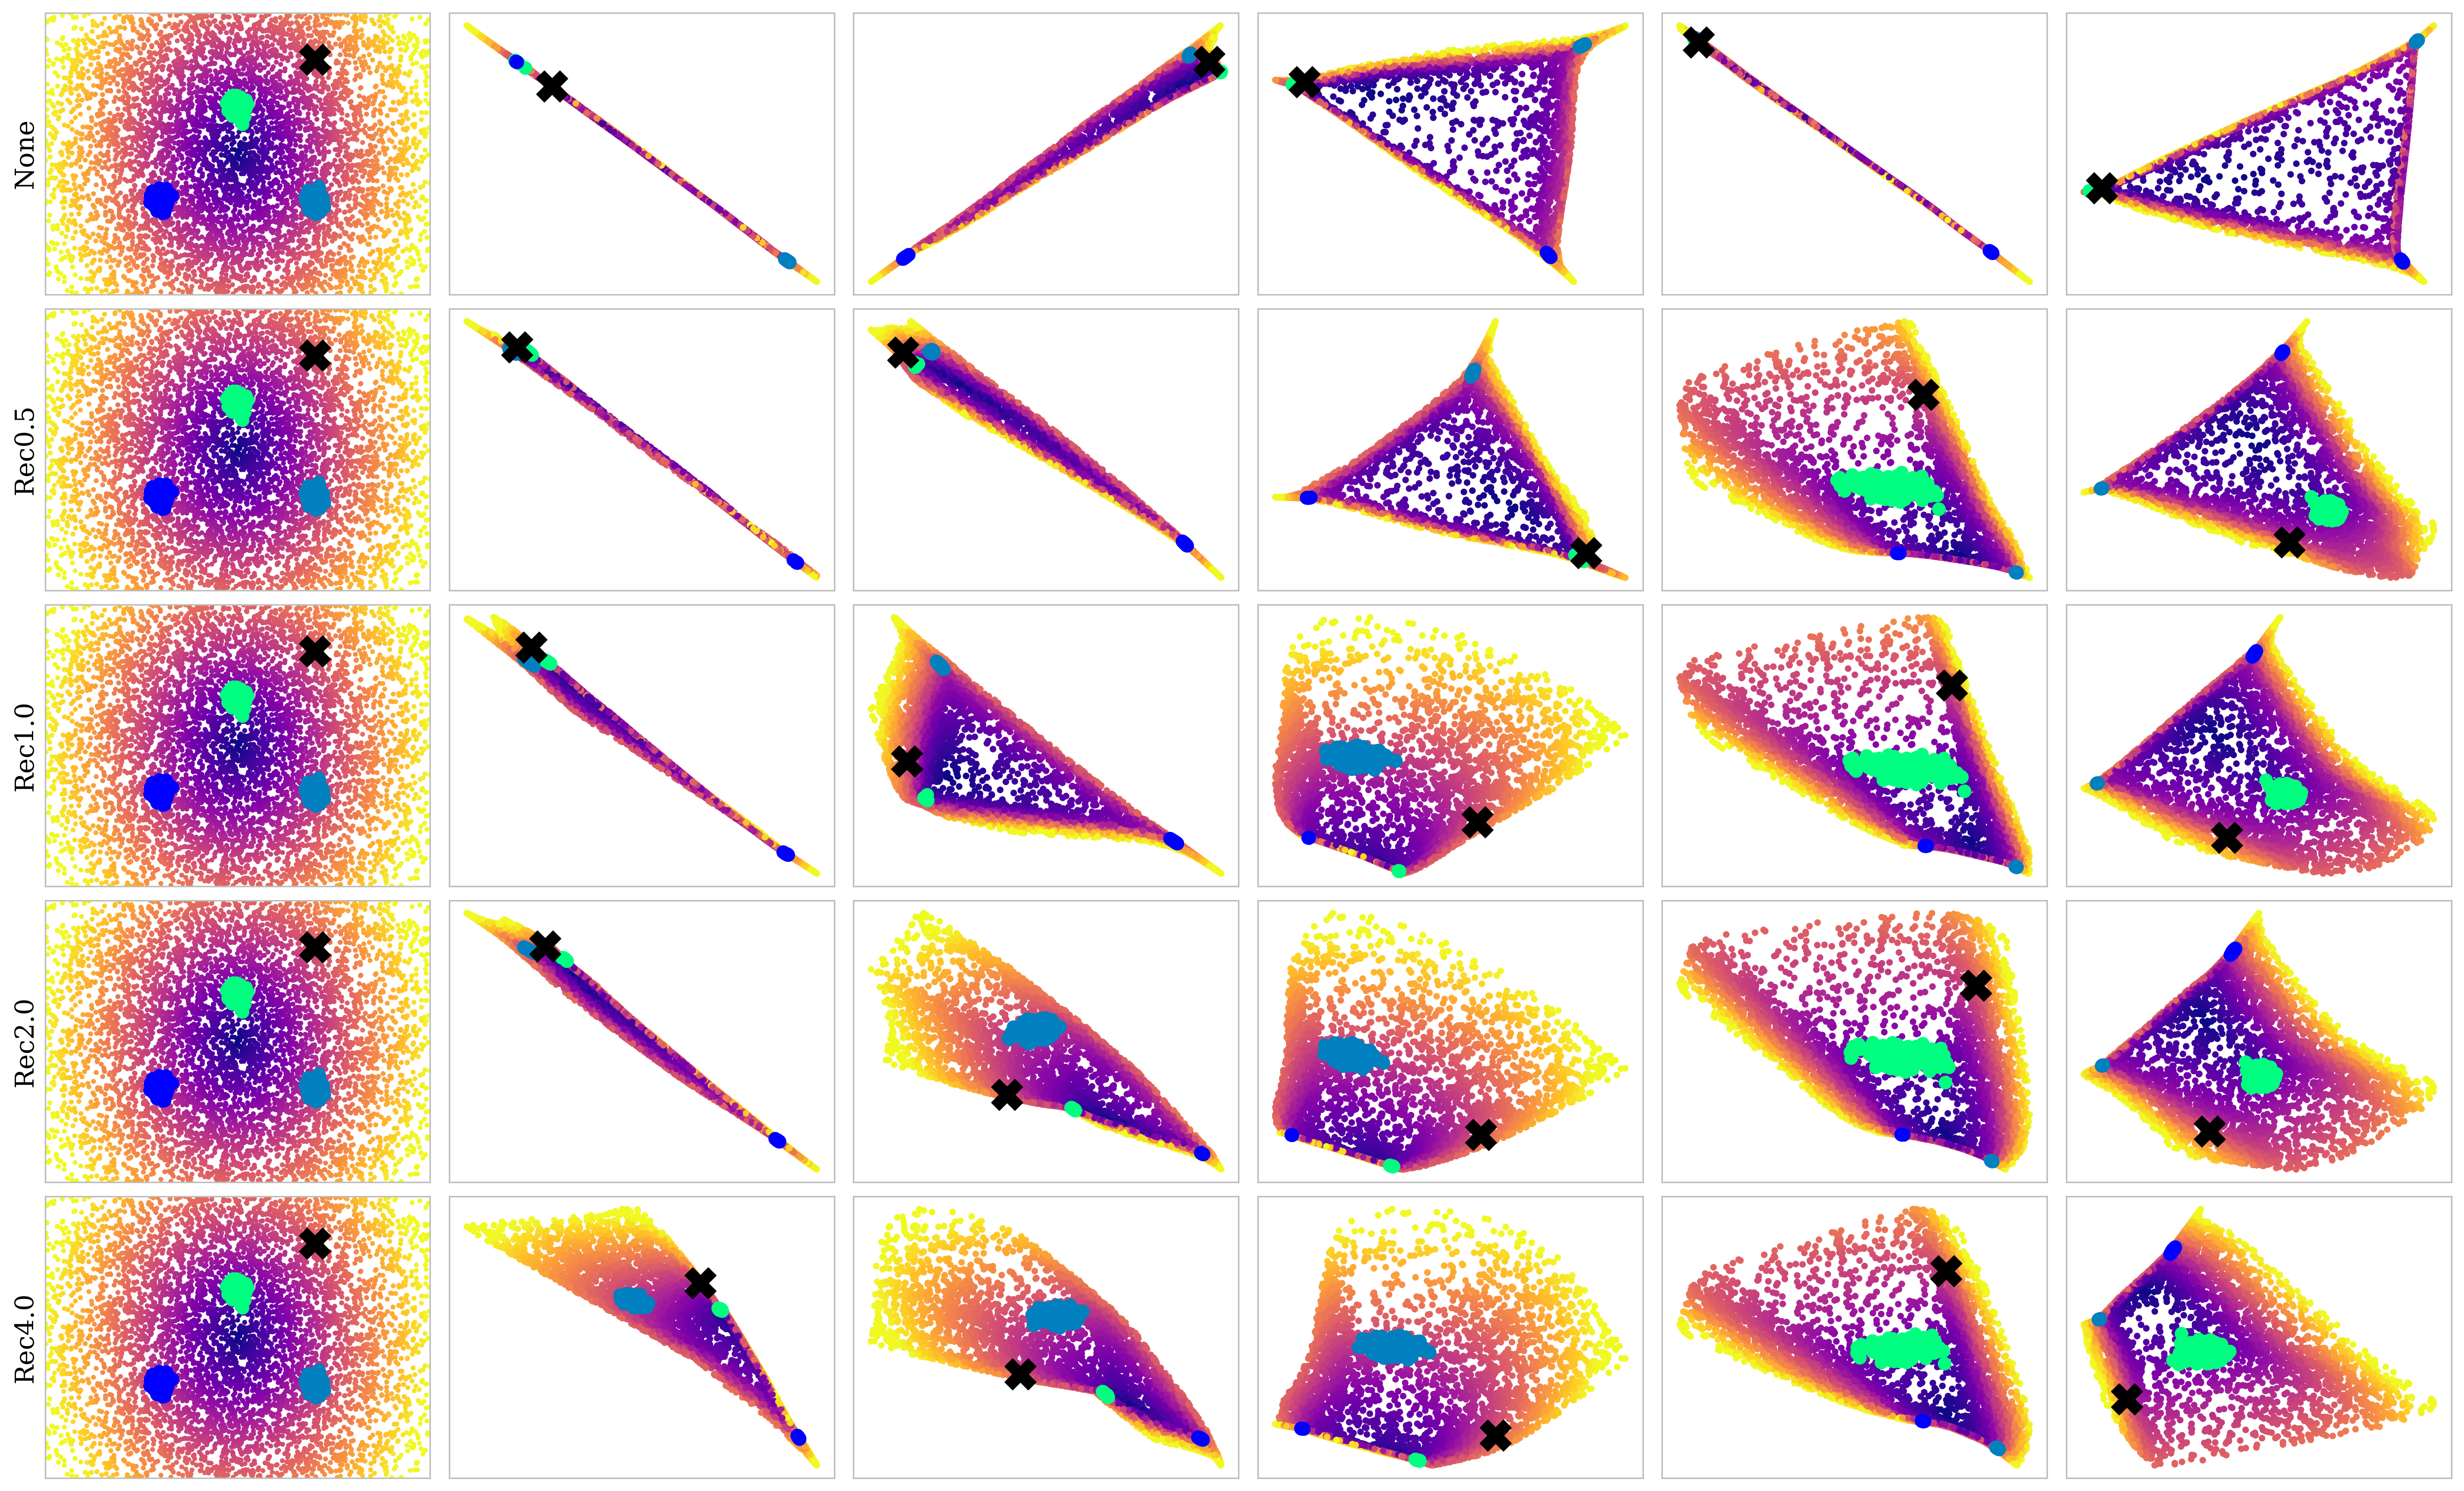
\includegraphics[width=0.8\textwidth]{sections/008_iclr2023/figures/toy/blob2/rec_collapse.png}
        \caption{Reconstruction}
        \label{fig:rec_toy_collapse}
    \end{subfigure}
    \caption{\textbf{Regularization constraint toy dataset feature collapse with NatPN.} Similarly to \citep{due}, we run the toy experiment where the first column represent two Gaussian class of data, sharing the same y-axis center to trigger the \textit{feature collapse} phenomenon, and a grid of unrelated point to simulate the space distorsion (colors are based on the Gaussian's generating distribution). 
    Each row is a different setting, e.g. \textit{bi1.0} is the bi-Lipschitz constraint with the Lipschitz constant $c = 1$ and \textit{rec1.0} is the reconstruction term with $\lambda=1$. Each column is a different seed initialization. Results are the same as \ref{fig:bi_toy}. Larger Lipschitz constant \textit{c} reverts back to the residual connection, and reconstruction regularization collapses the 2D dimension into one single dimension. }
    \label{fig:toy_collpase}
\end{figure}


% -----------------------------------


\begin{figure}[!htb]
    \centering
    \begin{subfigure}[b]{\textwidth}
        \includegraphics[width=\textwidth]{sections/008_iclr2023/figures/latent_ood_mnist.pdf}
        \caption{MNIST}
        \label{fig:latent_ood_mnist}
    \end{subfigure}
    \begin{subfigure}[b]{\textwidth}
        \includegraphics[width=\textwidth]{sections/008_iclr2023/figures/latent_ood_cifar10.pdf}
        \caption{CIFAR10}
        \label{fig:latent_ood_cifar10}
    \end{subfigure}
    \begin{subfigure}[b]{\textwidth}
        \includegraphics[width=\textwidth]{sections/008_iclr2023/figures/latent_ood_cifar100.pdf}
        \caption{CIFAR100}
        \label{fig:latent_ood_cifar100}
    \end{subfigure}
    \begin{subfigure}[b]{\textwidth}
        \includegraphics[width=\textwidth]{sections/008_iclr2023/figures/latent_ood_camelyon_id.pdf}
        \caption{Camelyon ID}
        \label{fig:latent_ood_camelyon}
    \end{subfigure}
    
    \caption{\textbf{Latent dimension OOD detection.} For each training dataset we show the uncertainty estimation results on the corresponding OOD dataset. NatPN encounters numerical instabilities with high latent dimension on Camelyon dataset, while DUE is less sensitive to the variation.}
    \label{fig:latent_ood}
\end{figure}


\begin{figure}[!htb]
    \centering
    \begin{subfigure}[b]{\textwidth}
        \includegraphics[width=\textwidth]{sections/008_iclr2023/figures/bi_bar_ood_mnist.pdf}
        \caption{MNIST}
        \label{fig:bi_bar_ood_mnist}
    \end{subfigure}
    \begin{subfigure}[b]{\textwidth}
        \includegraphics[width=\textwidth]{sections/008_iclr2023/figures/bi_bar_ood_cifar10.pdf}
        \caption{CIFAR10}
        \label{fig:bi_bar_ood_cifar10}
    \end{subfigure}
    \begin{subfigure}[b]{\textwidth}
        \includegraphics[width=\textwidth]{sections/008_iclr2023/figures/bi_bar_ood_cifar100.pdf}
        \caption{CIFAR100}
        \label{fig:bi_bar_ood_cifar100}
    \end{subfigure}
    \begin{subfigure}[b]{\textwidth}
        \includegraphics[width=\textwidth]{sections/008_iclr2023/figures/bi_bar_ood_camelyon_id.pdf}
        \caption{Camelyon ID}
        \label{fig:bi_bar_ood_camelyon}
    \end{subfigure}
    
    \caption{\textbf{Bi-lipschitz OOD detection.} For each training dataset we show the uncertainty estimation results on the corresponding OOD dataset. Bi-Lipschitz improvements are not consistent across different OOD datasets. }
    \label{fig:bi_ood}
\end{figure}


\begin{figure}[!htb]
    \centering
    \begin{subfigure}[b]{\textwidth}
        \includegraphics[width=\textwidth]{sections/008_iclr2023/figures/reconst_ood_mnist.pdf}
        \caption{MNIST}
        \label{fig:rec_ood_mnist}
    \end{subfigure}
    \begin{subfigure}[b]{\textwidth}
        \includegraphics[width=\textwidth]{sections/008_iclr2023/figures/reconst_ood_cifar10.pdf}
        \caption{CIFAR10}
        \label{fig:rec_ood_cifar10}
    \end{subfigure}
    \begin{subfigure}[b]{\textwidth}
        \includegraphics[width=\textwidth]{sections/008_iclr2023/figures/reconst_ood_cifar100.pdf}
        \caption{CIFAR100}
        \label{fig:rec_ood_cifar100}
    \end{subfigure}
    
    \caption{\textbf{Reconstruction regularization OOD detection.} Increasing the weight coefficient of the reconstruction loss term improved the OOD detection of NatPN in MNIST. However, we did not observe improvements on more complex datasets such as CIFAR.}
    \label{fig:rec_ood}
\end{figure}


\begin{figure}[!htb]
    \centering
    \includegraphics[width=0.8\linewidth]{sections/008_iclr2023/figures/reconst_samples.png}
    \caption{\textbf{Reconstruction regularization CIFAR samples.} (left) The original input (right) the reconstructed input after NatPN's joint training phase. The reconstruction discards detailed information compared to the original input. }
    \label{fig:rec_samples}
\end{figure}


\begin{table}[!htb]
\centering
\caption{\textbf{Encoder architecture OOD detection.} For each training dataset we show the uncertainty estimation results on the corresponding OOD dataset. We observe that new architectures (EfficientNet, Swin) have consistently better results. Interestingly, the transformer based model Swin, is not able to detect out-of-domain data, which should be easy in principle.}
\label{tab:encoder_architecture_ood}
\tiny
\begin{tabular}{lllccc}
    \toprule
    \textbf{Model} &\textbf{OOD Data} &\textbf{Architecture} &\textbf{OOD Alea. ($\uparrow$)} &\textbf{OOD Epis. ($\uparrow$)} &\textbf{OOD Pred. ($\uparrow$)} \\
    \midrule
    \multirow{20}{*}{NatPN} &\multirow{4}{*}{SVHN} &ResNet18 &\textbf{89.90 $\pm$ 1.22} &78.14 $\pm$ 3.13 &\textbf{89.90 $\pm$ 1.22} \\
    & &ResNet50 &89.34 $\pm$ 0.66 &92.02 $\pm$ 0.49 &89.34 $\pm$ 0.66 \\
    & &EfficientNet\_V2\_S &88.65 $\pm$ 0.68 &92.52 $\pm$ 0.60 &88.65 $\pm$ 0.68 \\
    & &Swin\_T &87.73 $\pm$ 1.36 &\textbf{94.17 $\pm$ 0.74} &87.73 $\pm$ 1.36 \\
    \cmidrule[0.1pt](lr){2-6}
    &\multirow{4}{*}{STL10} &ResNet18 &\textbf{90.99 $\pm$ 0.37} &83.90 $\pm$ 0.59 &\textbf{90.99 $\pm$ 0.37} \\
    & &ResNet50 &85.46 $\pm$ 0.50 &90.76 $\pm$ 0.31 &85.46 $\pm$ 0.50 \\
    & &EfficientNet\_V2\_S &88.68 $\pm$ 0.62 &91.11 $\pm$ 0.47 &88.68 $\pm$ 0.62 \\
    & &Swin\_T &85.44 $\pm$ 0.56 &\textbf{92.16 $\pm$ 0.40} &85.44 $\pm$ 0.56 \\
    \cmidrule[0.1pt](lr){2-6}
    &\multirow{4}{*}{CelebA} &ResNet18 &66.46 $\pm$ 3.48 &50.61 $\pm$ 2.14 &66.46 $\pm$ 3.48 \\
    & &ResNet50 &59.30 $\pm$ 3.77 &64.80 $\pm$ 2.15 &59.30 $\pm$ 3.77 \\
    & &EffNet\_V2\_S &\textbf{67.04 $\pm$ 1.74} &66.29 $\pm$ 1.45 &\textbf{67.04 $\pm$ 1.74} \\
    & &Swin\_T &63.60 $\pm$ 2.16 &\textbf{72.80 $\pm$ 1.00} &63.60 $\pm$ 2.16 \\
    \cmidrule[0.1pt](lr){2-6}
    &\multirow{4}{*}{Camelyon} &ResNet18 &90.09 $\pm$ 4.43 &96.28 $\pm$ 1.06 &90.09 $\pm$ 4.43 \\
    & &ResNet50 &90.64 $\pm$ 2.47 &97.82 $\pm$ 0.56 &90.64 $\pm$ 2.47 \\
    & &EfficientNet\_V2\_S &94.56 $\pm$ 0.79 &97.42 $\pm$ 0.44 &94.56 $\pm$ 0.79 \\
    & &Swin\_T &\textbf{95.43 $\pm$ 1.47} &\textbf{98.71 $\pm$ 0.50} &\textbf{95.43 $\pm$ 1.47} \\
    \cmidrule[0.1pt](lr){2-6}
    &\multirow{4}{*}{SVHN OODom.} &ResNet18 &\textbf{100.00 $\pm$ 0.00} &\textbf{100.00 $\pm$ 0.00} &\textbf{100.00 $\pm$ 0.00} \\
    & &ResNet50 &\textbf{100.00 $\pm$ 0.00} &\textbf{100.00 $\pm$ 0.00} &\textbf{100.00 $\pm$ 0.00} \\
    & &EfficientNet\_V2\_S &\textbf{100.00 $\pm$ 0.00} &\textbf{100.00 $\pm$ 0.00} &\textbf{100.00 $\pm$ 0.00} \\
    & &Swin\_T &97.37 $\pm$ 0.29 &93.31 $\pm$ 1.42 &97.37 $\pm$ 0.29 \\
    \midrule
    \multirow{20}{*}{DUE} &\multirow{4}{*}{SVHN} &ResNet18 &- &- &88.77 $\pm$ 0.28 \\
    & &ResNet50 &- &- &92.18 $\pm$ 0.11 \\
    & &EfficientNet\_V2\_S &- &- &90.95 $\pm$ 0.53 \\
    & &Swin\_T &- &- &\textbf{93.62 $\pm$ 0.39} \\
    \cmidrule[0.1pt](lr){2-6}
    &\multirow{4}{*}{STL10} &ResNet18 &- &- &\textbf{90.66 $\pm$ 0.48} \\
    & &ResNet50 &- &- &89.56 $\pm$ 0.53 \\
    & &EfficientNet\_V2\_S &- &- &89.08 $\pm$ 0.39 \\
    & &Swin\_T &- &- &89.73 $\pm$ 0.36 \\
    \cmidrule[0.1pt](lr){2-6}
    &\multirow{4}{*}{CelebA} &ResNet18 &- &- &64.75 $\pm$ 1.44 \\
    & &ResNet50 &- &- &72.19 $\pm$ 1.42 \\
    & &EffNet\_V2\_S &- &- &\textbf{72.28 $\pm$ 1.76} \\
    & &Swin\_T &- &- &69.37 $\pm$ 0.67 \\
    \cmidrule[0.1pt](lr){2-6}
    &\multirow{4}{*}{Camelyon} &ResNet18 &- &- &96.01 $\pm$ 1.13 \\
    & &ResNet50 &- &- &97.28 $\pm$ 0.47 \\
    & &EfficientNet\_V2\_S &- &- &94.82 $\pm$ 0.65 \\
    & &Swin\_T &- &- &\textbf{99.33 $\pm$ 0.14} \\
    \cmidrule[0.1pt](lr){2-6}
    &\multirow{4}{*}{SVHN OODom.} &ResNet18 &- &- &\textbf{100.00 $\pm$ 0.00} \\
    & &ResNet50 &- &- &\textbf{100.00 $\pm$ 0.00} \\
    & &EfficientNet\_V2\_S &- &- &\textbf{100.00 $\pm$ 0.00} \\
    & &Swin\_T &- &- &97.47 $\pm$ 0.22 \\
    \bottomrule
\end{tabular}
\end{table}

% PRIOR -----------------------------------
\section{Prior for DUMs}
\label{sec:prior}

In this section, we study the effect that the prior component has in DUMs. More specifically, we investigate the relationships between aleatoric uncertainty and the prior specified for DUMs. In particular, this is motivated by \citet{kapoor2022prior_cpe} which shows that using priors that forces model to be confident on the training data points can improve its performance by explicitly accounting for aleatoric uncertainty.
To this end, we look at \textit{entropy regularization} defining a training prior in the loss, \textit{prior evidence} and \textit{kernel function} defining a functional prior in the uncertainty head.

\textbf{Prior.} We compare different prior specifications including \textit{entropy regularization} defining a training prior in the loss, \textit{prior evidence} and \textit{kernel function} defining a functional prior in the uncertainty head. Entropy regularization is the entropy term $H(Q)$ in the Bayesian loss used to train NatPN which encourages a (uniform) prior distributions with high entropy \citep{NatPN2021}. We control the strength of the regularization factor $\lambda$. Further, NatPN also explicitly defines a prior via the parameters $\chi^{prior}$ and $n^{prior}$. While  $\chi^{prior}$ defines the default categorical prediction via a uniform categorical distribution, the evidence parameter $n^{prior}$ defines the prior number of pseudo-observations and can be varied. Finally, we vary the prior of DUE by using different kernel functions in the learned GP including Matern kernel, RQ kernel, and RBF \citep{gp-for-ml}. \underline{\textit{Observation:}} Contrary to other Bayesian neural networks \citep{kapoor2022prior_cpe}, we observe that predictive and uncertainty performances of DUMs are not very sensitive to the prior specification (see \cref{fig:prior_ood,fig:prior_ood_brier,tab:kernel}), thus suggesting a higher robustness to prior mispecification. Nonetheless, a too strong entropy regularization toward an uniform prior degrades more performance of DUMs trained on dataset with low label noise than on high label noise. This suggests that a too high discrepancy between the model prior and the dataset aleatoric uncertainties can impact performance.

\begin{figure}[!htb]
    \centering
    \includegraphics[width=\textwidth]{sections/008_iclr2023/figures/prior_entropy_acc_pred.pdf}
    \includegraphics[width=\textwidth]{sections/008_iclr2023/figures/prior_pseudo_acc_pred.pdf}
    
    \caption{Results of enforcing different \textbf{prior} in NatPN on CIFAR100 by changing the (top) \textit{entropy regularization} $\lambda$ and the (bottom) \textit{evidence prior} $n^{prior}$. Different priors do not lead consistent results improvements.}
    \label{fig:prior_ood}
\end{figure}
 \vspace{-3mm}
\begin{table}[!htp]\centering
\caption{Results of enforcing different \textbf{prior} in DUE on CIFAR100 and Camelyon by changing the kernel function. OOD results are averaged over OOD datasets. Different priors lead to similar performance. }
\label{tab:kernel}
\vspace{-0mm}
\tiny
\resizebox{0.9\textwidth}{!}{%
\begin{tabular}{lcccccc}\toprule
&\multicolumn{3}{c}{\textbf{CIFAR100}} &\multicolumn{3}{c}{\textbf{Camelyon}} \\
\cmidrule(lr){2-4}\cmidrule(lr){5-7}
\textbf{Kernel} &\textbf{Accuracy ($\uparrow$)} &\textbf{Brier Score ($\downarrow$)} &\textbf{OOD Pred. ($\uparrow$)} &\textbf{Accuracy ($\uparrow$)} &\textbf{Brier Score ($\downarrow$)} &\textbf{OOD Pred. ($\uparrow$)} \\
\midrule
Matern52 &71.80 $\pm$ 0.18 &41.37 $\pm$ 0.24 &75.90 $\pm$ 1.18 &79.81 $\pm$ 2.72 &32.46 $\pm$ 3.22 &58.86 $\pm$ 6.20 \\
Matern32 &71.80 $\pm$ 0.21 &41.62 $\pm$ 0.22 &\textbf{76.15 $\pm$ 1.18} &80.23 $\pm$ 2.71 &32.77 $\pm$ 3.20 &58.50 $\pm$ 5.83 \\
Matern12 &71.70 $\pm$ 0.18 &43.10 $\pm$ 0.22 &75.70 $\pm$ 1.19 &79.30 $\pm$ 2.96 &32.67 $\pm$ 3.28 &\textbf{59.13 $\pm$ 6.39} \\
RQ &71.83 $\pm$ 0.19 &\textbf{41.16 $\pm$ 0.25} &75.93 $\pm$ 1.21 &80.31 $\pm$ 2.55 &32.22 $\pm$ 3.14 &58.69 $\pm$ 6.09 \\
RBF &\textbf{71.85 $\pm$ 0.19} &41.17 $\pm$ 0.24 &76.14 $\pm$ 1.19 &\textbf{80.45 $\pm$ 2.49} &\textbf{32.13 $\pm$ 3.11} &58.86 $\pm$ 5.91 \\
\bottomrule
\end{tabular}
}
\vspace{-3mm}
\end{table}


% \begin{table}[!htp]\centering
% \caption{\textbf{Uncertainty Head Prior.} (top) NatPN with a more expressive uncertainty head obtain significantly better performance. (bottom) DUE changing its uncertainty headoesn't have much effects. The reported OOD results are an average over all the independent OOD dataset result.}
% \label{tab:kernel}
% \tiny
% \begin{tabular}{lccccccccc}\toprule
% &\multicolumn{4}{c}{\textbf{CIFAR100}} &\multicolumn{4}{c}{\textbf{Camelyon}} \\
% \cmidrule(lr){2-5}\cmidrule(lr){6-9}
% \textbf{Head} &\textbf{Accuracy} &\textbf{Brier score} &\textbf{OOD Pred.} &\textbf{OOD Epis.} &\textbf{Accuracy} &\textbf{Brier score} &\textbf{OOD Pred.} &\textbf{OOD Epis.} \\
% \midrule
% Radial &71.09 $\pm$ 0.21 &52.27 $\pm$ 0.28 &72.84 $\pm$ 1.82 &50.95 $\pm$ 2.16 &83.14 $\pm$ 0.93 &24.55 $\pm$ 1.91 &60.27 $\pm$ 5.29 &69.16 $\pm$ 7.94 \\
% \textbf{NSF-R} &\textbf{71.61 $\pm$ 0.07} &\textbf{43.44 $\pm$ 0.11} &\textbf{73.54 $\pm$ 1.69} &\textbf{72.85 $\pm$ 1.25} &\textbf{89.84 $\pm$ 7.93} &\textbf{12.52 $\pm$ 6.17} &\textbf{64.14 $\pm$ 10.42} &\textbf{81.33 $\pm$ 8.78} \\

% \midrule
% \midrule

% Matern52 &71.80 $\pm$ 0.18 &41.37 $\pm$ 0.24 &75.90 $\pm$ 1.18 &- &79.81 $\pm$ 2.72 &32.46 $\pm$ 3.22 &58.86 $\pm$ 6.20 &- \\
% Matern32 &71.80 $\pm$ 0.21 &41.62 $\pm$ 0.22 &\textbf{76.15 $\pm$ 1.18} &- &80.23 $\pm$ 2.71 &32.77 $\pm$ 3.20 &58.50 $\pm$ 5.83 &- \\
% Matern12 &71.70 $\pm$ 0.18 &43.10 $\pm$ 0.22 &75.70 $\pm$ 1.19 &- &79.30 $\pm$ 2.96 &32.67 $\pm$ 3.28 &\textbf{59.13 $\pm$ 6.39} &- \\
% RQ &71.83 $\pm$ 0.19 &\textbf{41.16 $\pm$ 0.25} &75.93 $\pm$ 1.21 &- &80.31 $\pm$ 2.55 &32.22 $\pm$ 3.14 &58.69 $\pm$ 6.09 &- \\
% RBF &\textbf{71.85 $\pm$ 0.19} &41.17 $\pm$ 0.24 &76.14 $\pm$ 1.19 &- &\textbf{80.45 $\pm$ 2.49} &\textbf{32.13 $\pm$ 3.11} &58.86 $\pm$ 5.91 &- \\
% \bottomrule
% \end{tabular}
% \end{table}
\section{Conclusion}
\label{sec:conclusion_008}

This chapter analyzes robustness of uncertainty estimation by DBU models and answers multiple questions in this context. Our results show: (1) While uncertainty estimates are a good indicator to identify correctly classified samples on unperturbed data, performance decrease drastically on perturbed data-points. (2) None of the Dirichlet-based uncertainty models is able to detect PGD label attacks against the class prediction by uncertainty estimation, regardless of the used uncertainty measure. (3) Detecting OOD samples and distinguishing between ID-data and OOD-data is not robust. (4) Applying median smoothing to  uncertainty estimates increases robustness of DBU models w.r.t. all analyzed tasks, while adversarial training based on label or uncertainty attacks resulted in minor improvements. 






\newpage
\bibliography{iclr2023_conference}
\bibliographystyle{iclr2023_conference}

\newpage
\section{Appendix}
\label{sec:appendix}

%\subsection{Dirichlet-based uncertainty models}
%
%In this section, we provide details on the losses used by each DBU model. \PostNet uses a Bayesian loss which can be expressed as follows:
%
%\begin{equation}
%\begin{aligned}
%    L_{\mathrm{\PostNet}} &= \frac{1}{N} \sum_i \E_{q(p\dataix)}  [\mathrm{CE} (p\dataix, y\dataix)] - H(q\dataix)
%\end{aligned}
%\end{equation}
%where $\mathrm{CE}$ denotes the cross-entropy. Both the expectation term (i.e. $\E_{q(p\dataix)}  [\mathrm{CE} (p\dataix, y\dataix)]$) and the entropy term (i.e. $H(q\dataix)$) can be computed in closed-form \citep{charpentier2020}. \PriorNet uses a loss composed of two KL divergence terms for ID and OOD data: 
%\begin{equation}
%\begin{aligned}
%    L_{\mathrm{\PriorNet}} &= \frac{1}{N} \left[\sum_{\vx\dataix \in \text{ID data}}  [\mathrm{KL} [\mathrm{Dir} (\alpha^{\mathrm{ID}}) || q\dataix]]  \right. \\
%                           &+ \left.\sum_{\vx\dataix \in OOD data} [\mathrm{KL} [\mathrm{Dir} (\alpha^{\mathrm{OOD}}) || q\dataix]]\right]. \\
%\end{aligned}
%\end{equation}
%Both KL divergences terms can be computed in closed-form \citep{malinin2019}. The precision $\alpha^{\mathrm{ID}}$ and $\alpha^{\mathrm{OOD}}$ are hyper-parameters. The precision $\alpha^{\mathrm{ID}}$ is usually set to $1e^{1}$ for the correct class and $1$ otherwise. The precision $\alpha^{\mathrm{OOD}}$ is usually set to $\mathbf{1}$. \DDNet uses use the Dirichlet likelihood of soft labels produce by an ensemble of $M$ neural networks:
%\begin{equation}
%\begin{aligned}
%    L_{\mathrm{\DDNet}} &= - \frac{1}{N}  \sum_i \sum_{m=1}^{M} [\ln q\dataix(\pi^{im})] \\
%\end{aligned}
%\end{equation}
%where $\pi^{im}$ denotes the soft-label of $m$th neural network. The Dirichlet likelihood can be computed in closed-form \citep{malinin2019ensemble}. \EvNet uses the expected mean square error between the one-hot encoded label and the predicted categorical distribution:
%
%\begin{equation}
%\begin{aligned}
%    L_{\mathrm{\EvNet}} &= \frac{1}{N} \sum_i \E_{\vp\dataix \sim \text{Dir}(\bm{\alpha}\dataix)}||\vy*\dataix - \vp\dataix||^2 \\
%\end{aligned}
%\end{equation}
%where $\vy*\dataix$ denotes the one-hot encoded label. The expected MSE loss can also be computed in closed form \citep{sensoy2018}.
%For more details please have a look at the original paper on \PriorNet \citep{malini2018}, \PostNet \citep{charpentier2020}, \DDNet \citep{malinin2019} and \EvNet \citep{sensoy2018}. 


\subsection{Closed-form computation of uncertainty measures \& Uncertainty attacks}
\label{subsec:appendix_measurecomp}

Dirichlet-based uncertainty models allow to compute several uncertainty measures in closed form (see \citep{malini2018} for a derivation). As proposed by \cite{malini2018}, we use precision~$m_{\alpha_0}$, differential entropy~$m_{\mathrm{diffE}}$ and mutual information~$m_{\mathrm{MI}}$ to estimate uncertainty on predictions.

The differential entropy $m_{\mathrm{diffE}}$ of a DBU model reaches its maximum value for equally probable categorical distributions and thus, a on flat Dirichlet distribution. It is a measure for distributional uncertainty and expected to be low on ID data, but high on OOD data. 
%
\begin{equation}
\begin{aligned}
	%m_{\mathrm{diffE}}  &= \sum_c^K \ln \Gamma (\alpha_c) - \ln \Gamma (\alpha_0) - \sum_c^K (\alpha_c -1) \cdot (\Psi (\alpha_c) - \Psi (\alpha_0))
	m_{\mathrm{diffE}}  = &\sum_c^K \ln \Gamma (\alpha_c) - \ln \Gamma (\alpha_0) \\
	&- \sum_c^K (\alpha_c -1) \cdot (\Psi (\alpha_c) - \Psi (\alpha_0))
\end{aligned}
\end{equation}
%
where $\alpha$ are the parameters of the Dirichlet-distribution, $\Gamma$ is the Gamma function and $\Psi$ is the Digamma function. 


The mutual information $m_{\mathrm{MI}}$ is the difference between the total uncertainty (entropy of the expected distribution) and the expected uncertainty on the data (expected entropy of the distribution). This uncertainty is expected to be low on ID data and high on OOD data. 
%
\begin{equation}
\begin{aligned}
	m_{\mathrm{MI}}  &= - \sum_{c=1}^{K} \frac{\alpha_c}{\alpha_0} \left( \ln \frac{\alpha_c}{\alpha_0} - \Psi(\alpha_c +1) + \Psi (\alpha_0 +1) \right)
\end{aligned}
\end{equation}

Furthermore, we use the precision~$\alpha_0$ to measure uncertainty, which is expected to be high on ID data and low on OOD data.
%
\begin{equation}
\begin{aligned}
	m_{\alpha_0}        &= \alpha_0 = \sum_{c=1}^{K} \alpha_c 
\end{aligned}
\end{equation}


As these uncertainty measures are computed in closed form and it is possible to obtain their gradients, we use them (i.e. $m_{\mathrm{diffE}}$, $m_{\mathrm{MI}}$, $m_{\alpha_0}$) are target function of our uncertainty attacks. Changing the attacked target function allows us to use a wide range of gradient-based attacks such as FGSM attacks, PGD attacks, but also more sophisticated attacks such as Carlini-Wagner attacks. 



\subsection{Details of the Experimental setup}
\label{subsec:exp_setup}

\textbf{Models.} We trained all models with a similar based architecture. We used namely 3 linear layers for vector data sets, 3 convolutional layers with size of 5 + 3 linear layers for MNIST and the VGG16 \cite{vgg} architecture with batch normalization for CIFAR10. All the implementation are performed using Pytorch \citep{pytorch}. We optimized all models using Adam optimizer. We performed early stopping by checking for loss improvement every 2 epochs and a patience of 10. The models were trained on GPUs (1 TB SSD).

We performed a grid-search for hyper-parameters for all models. The learning rate grid search was done in $[1e^{-5}, 1e^{-3}]$. For \PostNet, we used Radial Flows with a depth of 6 and a latent space equal to 6. Further, we performed a grid search for the regularizing factor in $[1e^{-7}, 1e^{-4}]$. For \PriorNet, we performed a grid search for the OOD loss weight in $[1, 10]$. For \DDNet, we distilled the knowledge of $5$ neural networks after a grid search in $[2, 5, 10, 20]$ neural networks. Note that it already implied a significant overhead at training compare to other models.

\textbf{Metrics.} For all experiments, we focused on using AUC-PR scores since it is well suited to imbalance tasks \citep{imbalance_apr} while bringing theoretically similar information than AUC-ROC scores \citep{apr_auroc}. We scaled all scores from $[0, 1]$ to $[0, 100]$. All results are average over 5 training runs using the best hyper-parameters found after the grid search.

\textbf{Data sets.} For vector data sets, we use 5 different random splits to train all models. We split the data in training, validation and test sets ($60\%$, $20\%$, $20\%$). 

We use the segment vector data set \cite{uci_datasets}, where the goal is to classify areas of images into $7$ classes (window, foliage, grass, brickface, path, cement, sky). We remove class window from ID training data to provide OOD training data to \PriorNet. Further, We remove the class 'sky' from training and instead use it as the OOD data set for OOD detection experiments. Each input is composed of $18$ attributes describing the image area. The data set contains $2,310$ samples in total.

We further use the Sensorless Drive vector data set \cite{uci_datasets}, where the goal is to classify extracted motor current measurements into $11$ different classes. We remove class 9 from ID training data to provide OOD training data to \PriorNet. We remove classes 10 and 11 from training and use them as the OOD dataset for OOD detection experiments. Each input is composed of $49$ attributes describing motor behaviour. The data set contains $58,509$ samples in total.

Additionally, we use the MNIST image data set \cite{mnist} where the goal is to classify pictures of hand-drawn digits into $10$ classes (from digit $0$ to digit $9$). Each input is composed of a $1 \times 28 \times 28$ tensor. The data set contains $70,000$ samples. For OOD detection experiments, we use FashionMNIST \cite{fashionmnist} and KMNIST \cite{kmnist} containing images of Japanese characters and images of clothes, respectively. FashionMNIST was used as training OOD for \PriorNet while KMNIST is used as OOD at test time.

Finally, we use the CIFAR10 image data set \cite{cifar10} where the goal is to classify a picture of objects into $10$ classes (airplane, automobile, bird, cat, deer, dog, frog, horse, ship, truck). Each input is a $3 \times 32 \times 32$ tensor. The data set contains $60,000$ samples. For OOD detection experiments, we use street view house numbers (SVHN) \cite{svhn}  and CIFAR100 \citep{cifar10} containing images of numbers and objects respectively. CIFAR100 was used as training OOD for \PriorNet while SVHN is used as OOD at test time.
 
\textbf{Perturbations.} For all label and uncertainty attacks, we used Fast Gradient Sign Methods and Project Gradient Descent. We tried 6 different attack radii $[0.0, 0.1, 0.2, 0.5, 1.0, 2.0, 4.0]$. These radii operate on the input space after data normalization. We bound perturbations by~$L_{\infty}$-norm or by~$L_2$-norm, with 
%
\begin{equation}
\begin{aligned}
	L_{\infty} (x) = \max_{i=1,\dots, D} \left|x_i\right| \mathrm{~~~~and~~~~}
	L_2 (x)        = (\sum_{i=1}^{D} x_i^2)^{0.5}.
\end{aligned}
\end{equation}
%
For $L_{\infty}$-norm it is obvious how to relate perturbation size~$\varepsilon$ with perturbed input images, because all inputs are standardized such that the values of their features are between~$0$ and~$1$.
A perturbation of size~$\varepsilon=0$ corresponds to the original input, while a perturbation of size~$\varepsilon=1$ corresponds to the whole input space and allows to change all features to any value. 

For~$L_2$-norm the relation between perturbation size~$\varepsilon$ and perturbed input images is less obvious. To justify our choice for~$\varepsilon$ w.r.t. this norm, we relate perturbations size~$\varepsilon_2$ corresponding to $L_2$-norm with perturbations size~$\varepsilon_{\infty}$ corresponding to $L_{\infty}$-norm. 
First, we compute~$\varepsilon_2$, such that the $L_2$-norm is the smallest super-set of the $L_{\infty}$-norm. Let us consider a perturbation of~$\varepsilon_{\infty}$. The largest~$L_2$-norm would be obtained if each feature is perturbed by~$\varepsilon_{\infty}$. Thus, perturbation~$\varepsilon_2$, such that $L_2$ encloses~$L_{\infty}$ is $\varepsilon_2 = (\sum_{i=1}^{D} \varepsilon_{\infty}^2)^{0.5} = \sqrt{D} \varepsilon_{\infty}$. For the MNIST-data set, with $D=28 \times 28$ input features $L_2$-norm with $\varepsilon_2=28$ encloses $L_{\infty}$-norm with~$\varepsilon_{\infty}=1$. 

Alternatively, $\varepsilon_2$ can be computes such that the volume spanned by~$L_2$-norm is equivalent to the one spanned by~$L_{\infty}$-norm. Using that the volume spanned by $L_{\infty}$-norm is $\varepsilon_{\infty}^D$ and the volume spanned by $L_2$-norm is 
$\frac{\pi^{0.5 D} \varepsilon_2^D}{\Gamma(0.5 D +1)}$ (where $\Gamma$ is the Gamma-function), we obtain volume equivalence if 
$\varepsilon_2 = \Gamma(0.5 D +1)^{\frac{1}{D}} \sqrt{\pi} \varepsilon_{\infty}$. For the MNIST-data set, with $D=28 \times 28$ input features $L_2$-norm with $\varepsilon_2 \approx 21.39$ is volume equivalent to $L_{\infty}$-norm with~$\varepsilon_{\infty}=1$.











\newpage 
\subsection{Additional Experiments}



Table~\ref{tab:acc_label_attack} and~\ref{tab:acc_label_attack_fgsm} illustrate that no DBU model maintains high accuracy under gradient-based label attacks. Accuracy under PGD attacks decreases more than under FGSM attacks, since PGD is stronger.  Interestingly Noise attacks achieve also good performances with increasing Noise standard deviation. Note that the attack is not constraint to be with a given radius for Noise attacks.



\begin{table*}[htbp!]
 	\centering
 	\caption{Accuracy under PGD label attacks.}
 	\begin{small}
 		\begin{tabular}{@{}rrrrrrrrc|crrrrrrr@{}}
 			\toprule
  			Att. Rad. & 0.0 & 0.1 & 0.2 & 0.5 & 1.0 & 2.0 & 4.0 & & & 0.0 & 0.1 & 0.2 & 0.5 & 1.0 & 2.0 & 4.0 \\
 			\midrule
 			& \multicolumn{7}{c}{MNIST} & & & \multicolumn{7}{c}{CIFAR10} \\
 			\PostNet  &  \bf{99.4} &  \bf{99.2} &  \bf{98.8} &  96.8 &  89.6 &  53.8 &  13.0 & &
 			          &  89.5 &  73.5 &  51.7 &  13.2 &   2.2 &   0.8 &  0.3 \\
 			\PriorNet &  99.3 &  99.1 &  \bf{98.8} &  97.4 &  \bf{93.9} &  \bf{75.3} &   4.8 & &
 			          &  88.2 &  \bf{77.8} &  \bf{68.4} &  \bf{54.0} &  \bf{37.9} &  \bf{17.5} &  \bf{5.1} \\
 		    \DDNet    &  \bf{99.4} &  99.1 &  \bf{98.8} &  \bf{97.5} &  91.6 &  48.8 &   0.2 & &
 		              &  86.1 &  73.9 &  59.1 &  20.5 &   1.5 &   0.0 &  0.0 \\
 		    \EvNet    &  99.2 &  98.9 &  98.4 &  96.8 &  92.4 &  73.1 &  \bf{40.9} & &
 		              &  \bf{89.8} &  71.7 &  48.8 &  11.5 &   2.7 &   1.5 &  0.4 \\
 		    \midrule
 		 & \multicolumn{7}{c}{Sensorless} & & & \multicolumn{7}{c}{Segment} \\
 			\PostNet  &  98.3 &  13.1 &   6.4 &   4.0 &  \bf{7.0} &  \bf{9.8} &  \bf{11.3} & &
 			          &  98.9 &  82.8 &  \bf{50.1} &  \bf{19.2} &  \bf{8.8} &  \bf{5.1} &  \bf{8.6}   \\
 			\PriorNet &  \bf{99.3} &  16.5 &   5.6 &   1.2 &  0.4 &  0.2 &   1.6 & &
 			          &  \bf{99.5} &  90.7 &  47.6 &   7.8 &  0.2 &  0.0 &  0.4 \\
 		    \DDNet    &  \bf{99.3} &  12.4 &   2.4 &   0.6 &  0.3 &  0.1 &   0.1 & &
 		              &  99.2 &  \bf{90.8} &  45.7 &   6.9 &  0.0 &  0.0 &  0.0 \\
 		    \EvNet    &  99.0 &  \bf{35.3} &  \bf{22.3} &  \bf{11.2} &  \bf{7.0} &  5.2 &   4.0 & &
 		              &  99.3 &  91.8 &  54.0 &  10.3 &  0.8 &  0.5 &  0.6 \\
 			\bottomrule
 		\end{tabular}
 	\end{small}
 	\label{tab:acc_label_attack}
\end{table*}



\begin{table*}[htbp!]
 	\centering
 	\caption{Accuracy under FGSM label attacks.}
 	\begin{small}
 		\begin{tabular}{@{}rrrrrrrrc|crrrrrrr@{}}
 			\toprule
 			Att. Rad. & 0.0 & 0.1 & 0.2 & 0.5 & 1.0 & 2.0 & 4.0 & & & 0.0 & 0.1 & 0.2 & 0.5 & 1.0 & 2.0 & 4.0 \\
 			\midrule
 			& \multicolumn{7}{c}{MNIST} & & & \multicolumn{7}{c}{CIFAR10} \\
 			\PostNet  & \bf{99.4} &  \bf{99.2} &  \bf{98.9} &  97.7 &  95.2 &  \bf{90.1} &  \bf{79.2} & &
 			          & 89.5 &  72.3 &  54.9 &  31.2 &  21.0 &  16.8 &  15.6 \\
 			\PriorNet & 99.3 &  99.1 &  \bf{98.9} &  97.7 &  \bf{95.8} &  93.2 &  76.7 & &
 			          & 88.2 &  \bf{77.3} &  \bf{70.1} &  \bf{59.4} &  \bf{52.3} &  \bf{48.5} &  \bf{46.8} \\
 		    \DDNet    & \bf{99.4} &  \bf{99.2} &  \bf{98.9} &  \bf{97.8} &  94.7 &  79.2 &  25.2 & &
 			          & 86.1 &  73.0 &  60.2 &  32.5 &  14.6 &   7.1 &   6.0 \\
 		    \EvNet    & 99.2 &  98.9 &  98.6 &  97.6 &  \bf{95.8} &  \bf{90.1} &  74.4 & &
 			          & \bf{89.8} &  71.4 &  54.5 &  29.6 &  18.1 &  14.4 &  13.4 \\
 		    \midrule
 		     & \multicolumn{7}{c}{Sensorless} & & & \multicolumn{7}{c}{Segment} \\
 			\PostNet  & 98.3 &  19.6 &  10.9 &  10.9 &  11.9 &  12.4 &  12.5 & &
 			          & 98.9 &  79.6 &  \bf{57.3} &  \bf{31.5} &  \bf{18.4} &  \bf{20.6} &  \bf{19.9} \\
 			\PriorNet & \bf{99.3} &  24.7 &  11.8 &   8.6 &   8.5 &   8.1 &   8.3 & &
 			          & \bf{99.5} &  85.5 &  40.5 &   8.9 &   0.4 &   0.3 &   0.2 \\
 		    \DDNet    & \bf{99.3} &  18.0 &   8.2 &   6.5 &   5.4 &   6.7 &   7.8 & &
 			          & 99.2 &  86.4 &  36.2 &  11.9 &   0.9 &   0.0 &   0.0 \\
 		    \EvNet    & 99.0 &  \bf{42.0} &  \bf{28.0} &  \bf{17.5} &  \bf{13.7} &  \bf{13.6} &  \bf{14.9} & &
 			          & 99.3 &  \bf{90.6} &  55.2 &  14.2 &   2.4 &   0.5 &   0.1 \\
 			\bottomrule
 		\end{tabular}
 	\end{small}
 	\label{tab:acc_label_attack_fgsm}
\end{table*}


\begin{table*}[htbp!]
 	\centering
 	\caption{Accuracy under Noise label attacks.}
 	\begin{small}
 		\begin{tabular}{@{}rrrrrrrrc|crrrrrrr@{}}
 			\toprule
 			%& \multicolumn{7}{c}{MNIST} & & & \multicolumn{7}{c}{CIFAR10} \\
 			%\cmidrule{2-8}  \cmidrule{11-16}
 			Noise Std & 0.0 & 0.1 & 0.2 & 0.5 & 1.0 & 2.0 & 4.0 & & & 0.0 & 0.1 & 0.2 & 0.5 & 1.0 & 2.0 & 4.0 \\
 			\midrule
 			& \multicolumn{7}{c}{MNIST} & & & \multicolumn{7}{c}{CIFAR10} \\
 			\PostNet  & \bf{99.4} &  \bf{98.6} &  91.8 &  \bf{14.9} &  \bf{1.3} &  \bf{0.1} &  0.0 & &
 			          & \bf{91.7} &  21.5 &  10.1 &   0.1 &   1.2 &  0.0 &  1.9 \\
 			\PriorNet & 99.3 &  98.5 &  \bf{95.7} &  14.4 &  0.0 &  0.0 &  0.0 & &
 			          & 87.7 &  \bf{28.1} &  \bf{11.2} &   9.7 &   5.0 &  \bf{8.5} &  \bf{9.0}\\
 		    \DDNet    & \bf{99.4} &  \bf{98.6} &  92.4 &  13.3 &  0.7 &  0.0 &  0.0 & &
 			          & 81.7 &  23.0 &  \bf{11.2} &  \bf{11.2} &  \bf{11.0} &  7.8 &  6.7 \\
 		    \EvNet    & 99.3 &  96.9 &  81.6 &  11.7 &  0.5 &  0.0 &  0.0 & &
 			          & 89.5 &  20.7 &  11.1 &   5.2 &   0.5 &  2.3 &  3.9 \\
 		    \midrule
 		     & \multicolumn{7}{c}{Sensorless} & & & \multicolumn{7}{c}{Segment} \\
 			\PostNet  & 98.1 &  0.1 &  \bf{3.7} &  \bf{11.7} &  \bf{11.7} &  \bf{11.7} &  \bf{11.7} & &
 			          & 98.5 &  39.4 &   3.9 &  \bf{1.8} &  \bf{12.1} &  \bf{20.3} &  \bf{22.1} \\
 			\PriorNet & \bf{99.3} &  0.2 &  0.0 &   0.0 &   0.0 &   0.3 &   2.4 & &
 			          & \bf{99.4} &  47.9 &   8.8 &  0.0 &   0.0 &   0.0 &   0.0 \\
 		    \DDNet    & 99.0 &  \bf{0.4} &  0.1 &   0.0 &   0.0 &   0.0 &   0.0 & &
 			          & 99.1 &  50.0 &  \bf{10.3} &  0.0 &   0.0 &   0.3 &   0.0 \\
 		    \EvNet    & 98.6 &  0.2 &  0.0 &   0.1 &   1.4 &   4.6 &   8.8 & &
 			          & 99.1 &  \bf{50.3} &  \bf{10.3} &  1.2 &   0.3 &   0.0 &   1.5 \\
 			\bottomrule
 		\end{tabular}
 	\end{small}
 	\label{tab:acc_label_attack_noise_attack}
\end{table*}

\clearpage
\subsubsection{Uncertainty estimation under label attacks}

\textbf{Is low uncertainty a reliable indicator of correct predictions?}

On non-perturbed data uncertainty estimates are an indicator of correctly classified samples, but if the input data is perturbed none of the DBU models maintains its high performance. Thus, uncertainty estimates are not a robust indicator of correctly labeled inputs. 

\begin{table*}[htbp!]
 	\centering
 	\caption{Distinguishing between correctly and wrongly predicted labels based on the differential entropy under PGD label attacks (AUC-PR).}
 	\begin{small}
 		\begin{tabular}{@{}rrrrrrrrc|crrrrrrr@{}}
 			\toprule
 			& \multicolumn{7}{c}{MNIST} & & & \multicolumn{7}{c}{Segment} \\
 			\cmidrule{2-8}  \cmidrule{11-16}
 			Att. Rad. & 0.0 & 0.1 & 0.2 & 0.5 & 1.0 & 2.0 & 4.0 & & & 0.0 & 0.1 & 0.2 & 0.5 & 1.0 & 2.0 & 4.0 \\
 			\midrule
 			%& \multicolumn{7}{c}{MNIST} & & & \multicolumn{7}{c}{Segment} \\
 			\PostNet  &  99.9 &   99.9 &  99.8 &  98.7 &  89.5 &  43.5 &   9.0 & & 
 			          &  99.9 &  77.6 &  31.6 &  \bf{11.1} &  \bf{5.3} &  \bf{4.4} &   8.7 \\
 			\PriorNet &  99.9 &   99.8 &  99.6 &  97.7 &  90.5 &  \bf{69.1} &   6.4 & & 
 			          &  \bf{100.0} &  \bf{96.8} &  44.5 &   4.5 &  0.4 &  0.0 &  \bf{15.2} \\
 		    \DDNet    &  \bf{100.0} &  \bf{100.0} &  \bf{99.9} &  \bf{99.7} &  \bf{97.6} &  50.2 &   0.1 & &
 		              &  \bf{100.0} &  \bf{96.8} &  \bf{54.0} &   4.3 &  0.0 &  0.0 &   0.0 \\
 		    \EvNet    &  99.6 &   99.3 &  98.7 &  96.1 &  88.8 &  63.1 &  \bf{31.7} & &
 		              &  \bf{100.0} &  95.9 &  44.3 &   5.9 &  0.8 &  0.6 &   0.7 \\
 			\bottomrule
 		\end{tabular}
 	\end{small}
 	\label{tab:conf_label_attack_2}
\end{table*}



\begin{table*}[htbp!]
 	\centering
 	\caption{Distinguishing between correctly and wrongly predicted labels based on the precision~$\alpha_0$ under PGD label attacks (AUC-PR).}
 	\begin{small}
 		\begin{tabular}{@{}rrrrrrrrc|crrrrrrr@{}}
 			\toprule
 			%& \multicolumn{7}{c}{MNIST} & & & \multicolumn{7}{c}{CIFAR10} \\
 			%\cmidrule{2-8}  \cmidrule{11-16}
 			Att. Rad. & 0.0 & 0.1 & 0.2 & 0.5 & 1.0 & 2.0 & 4.0 & & & 0.0 & 0.1 & 0.2 & 0.5 & 1.0 & 2.0 & 4.0 \\
 			\midrule
 			& \multicolumn{7}{c}{MNIST} & & & \multicolumn{7}{c}{CIFAR10} \\
            \PostNet  & \bf{100.0} &   99.9 &   99.7 &  98.2 &  87.9 &  39.1 &   6.9 & &
                      & \bf{98.7} &  88.6 &  56.2 &   7.8 &   1.2 &   0.4 &  0.3  \\
            \PriorNet &  99.9 &   99.8 &   99.6 &  97.7 &  90.4 & \bf{69.1} &   6.6  & &
                      &  92.9 &  77.7 &  60.5 & \bf{37.6} & \bf{24.9} & \bf{11.3} & \bf{3.0} \\
            \DDNet    & \bf{100.0} & \bf{100.0} & \bf{100.0} & \bf{99.8} & \bf{98.2} &  51.1 &   0.1  & &
                      &  97.6 & \bf{91.8} & \bf{78.3} &  18.1 &   0.8 &   0.0 &  0.0  \\
            \EvNet    &  99.6 &   99.2 &   98.6 &  95.7 &  88.6 &  63.6 & \bf{32.6} & &
                                  &  97.9 &  85.9 &  57.2 &  10.2 &   4.0 &   2.4 &  0.3  \\
 		    \midrule
 		     & \multicolumn{7}{c}{Sensorless} & & & \multicolumn{7}{c}{Segment} \\
            \PostNet  &  99.6 &   7.0 &   3.3 &  3.1 & \bf{6.9} & \bf{9.8} & \bf{11.3} & &
                      &  99.9 &  74.2 &  31.6 & \bf{11.1} & \bf{5.0} & \bf{4.2} & \bf{8.6} \\
            \PriorNet &  99.8 &  10.5 &   3.2 &  0.6 &  0.2 &  0.2 &   1.8 & &
                     & \bf{100.0} &  96.9 & \bf{45.2} &   4.4 &  0.4 &  0.0 &  1.2  \\
            \DDNet    &  99.8 &   8.7 &   1.3 &  0.3 &  0.2 &  0.1 &   0.2 & &
                    & \bf{100.0} & \bf{97.1} &  45.0 &   4.1 &  0.0 &  0.0 &  0.0 \\
            \EvNet    & \bf{99.9} & \bf{23.2} & \bf{13.2} & \bf{6.0} &  3.7 &  2.7 &   2.1 & &
                    & \bf{100.0} &  95.7 &  44.5 &   5.9 &  0.8 &  0.6 &  0.7 \\
 			\bottomrule
 		\end{tabular}
 	\end{small}
 	\label{tab:conf_label_attack_alpha}
\end{table*}



\begin{table*}[htbp!]
 	\centering
 	\caption{Distinguishing between correctly and wrongly predicted labels based on the mutual information under PGD label attacks (AUC-PR).}
 	\begin{small}
 		\begin{tabular}{@{}rrrrrrrrc|crrrrrrr@{}}
 			\toprule
 			%& \multicolumn{7}{c}{MNIST} & & & \multicolumn{7}{c}{CIFAR10} \\
 			%\cmidrule{2-8}  \cmidrule{11-16}
 			Att. Rad. & 0.0 & 0.1 & 0.2 & 0.5 & 1.0 & 2.0 & 4.0 & & & 0.0 & 0.1 & 0.2 & 0.5 & 1.0 & 2.0 & 4.0 \\
 			\midrule
 			& \multicolumn{7}{c}{MNIST} & & & \multicolumn{7}{c}{CIFAR10} \\
            \PostNet  & 99.7 &  99.7 &  99.6 &  99.2 &  92.4 &  40.0 &   6.9 & &
                      & \bf{97.3} &  84.5 &  56.2 &  12.2 &   2.4 &   0.7 &  0.3  \\
            \PriorNet &  99.9 &  99.8 &  99.6 &  97.7 &  90.3 & \bf{68.9} &   6.4  & &
                      &  82.7 &  65.6 &  51.4 & \bf{35.5} & \bf{24.4} & \bf{11.0} & \bf{2.9} \\
            \DDNet    & \bf{100.0} & \bf{99.9} & \bf{99.9} & \bf{99.7} & \bf{97.4} &  50.2 &   0.1  & &
                      &  96.9 & \bf{90.8} & \bf{77.2} &  18.8 &   0.8 &   0.0 &  0.0  \\
            \EvNet    &  97.8 &  97.0 &  95.7 &  92.6 &  86.1 &  62.3 & \bf{28.9} & &
                      &  91.3 &  72.4 &  47.9 &  11.4 &   1.6 &   0.9 &  1.6  \\
 		    \midrule
 		     & \multicolumn{7}{c}{Sensorless} & & & \multicolumn{7}{c}{Segment} \\
            \PostNet  &  99.3 &   7.0 &   3.3 &  3.3 & \bf{7.0} & \bf{9.8} &  11.3 & &
                      &  99.9 &  73.2 &  31.5 & \bf{11.1} & \bf{5.0} & \bf{4.3} & \bf{8.7} \\
            \PriorNet & \bf{99.8} &  10.5 &   3.2 &  0.6 &  0.2 &  0.1 & \bf{11.8} & &
                      & \bf{100.0} & \bf{96.6} & \bf{45.2} &   4.5 &  0.4 &  0.0 &  1.1  \\
            \DDNet    &  99.6 &   8.6 &   1.3 &  0.3 &  0.2 &  0.1 &   0.1 & &
                      & \bf{100.0} &  96.5 &  42.4 &   4.1 &  0.0 &  0.0 &  0.0 \\
            \EvNet    &  99.1 & \bf{22.0} & \bf{12.6} & \bf{5.9} &  3.7 &  2.7 &   2.2 & &
                      & \bf{100.0} &  90.5 &  41.0 &   5.9 &  0.8 &  0.6 &  0.7 \\
 			\bottomrule
 		\end{tabular}
 	\end{small}
 	\label{tab:conf_label_attack_mi}
\end{table*}


\begin{table*}[htbp!]
 	\centering
 	\caption{Distinguishing between correctly and wrongly predicted labels based on the differential entropy under FGSM label attacks (AUC-PR).}
 	\begin{small}
 		\begin{tabular}{@{}rrrrrrrrc|crrrrrrr@{}}
 			\toprule
 			%& \multicolumn{7}{c}{MNIST} & & & \multicolumn{7}{c}{CIFAR10} \\
 			%\cmidrule{2-8}  \cmidrule{11-16}
 			Att. Rad. & 0.0 & 0.1 & 0.2 & 0.5 & 1.0 & 2.0 & 4.0 & & & 0.0 & 0.1 & 0.2 & 0.5 & 1.0 & 2.0 & 4.0 \\
 			\midrule
 			& \multicolumn{7}{c}{MNIST} & & & \multicolumn{7}{c}{CIFAR10} \\
             \PostNet  & 99.9 &   99.9 &  99.8 &  99.4 &  97.8 & \bf{92.1} & \bf{83.2} & &
                      & \bf{98.5} &  88.7 &  68.9 &  31.0 &  18.6 &  15.5 &  16.7 \\
            \PriorNet & 99.9 &   99.9 &  99.7 &  98.3 &  94.1 &  88.5 &  78.6  & &
                      & 90.1 &  73.6 &  61.6 & \bf{46.1} & \bf{38.5} & \bf{35.6} & \bf{37.3} \\
            \DDNet    & \bf{100.0} & \bf{100.0} & \bf{99.9} & \bf{99.8} & \bf{98.7} &  86.4 &  23.0 & &
                      & 97.3 & \bf{90.6} & \bf{78.7} &  39.4 &  13.7 &   6.0 &   5.1 \\
            \EvNet    & 99.6 &   99.4 &  99.1 &  97.8 &  95.8 &  90.4 &  76.8 & &
                      & 98.0 &  86.2 &  67.4 &  32.7 &  19.9 &  18.2 &  19.7 \\		
 		    \midrule
 		     & \multicolumn{7}{c}{Sensorless} & & & \multicolumn{7}{c}{Segment} \\
             \PostNet  & 99.7 &  11.7 &   7.3 &   9.3 &  11.8 &  12.5 &  12.5 & &
                      & 99.9 &  73.6 &  40.6 & \bf{23.7} & \bf{17.2} & \bf{19.8} & \bf{20.2} \\
            \PriorNet & 99.8 &  21.4 &  10.4 &   8.5 &   9.0 &   9.2 &  10.3 & &
                      & \bf{100.0} &  93.7 &  37.7 &   5.8 &   1.1 &   0.9 &   0.8 \\
            \DDNet    & 99.7 &  18.5 &   5.4 &   4.3 &   4.2 &   5.7 &   7.9 & &
                      & \bf{100.0} & \bf{94.1} &  42.9 &   7.2 &   1.0 &   0.0 &   0.0 \\
            \EvNet    & \bf{99.9} & \bf{44.8} & \bf{29.2} & \bf{18.2} & \bf{15.1} & \bf{14.9} & \bf{15.5} & &
                      & \bf{100.0} &  93.7 & \bf{48.7} &   8.7 &   2.4 &   1.6 &   0.5 \\
 			\bottomrule
 		\end{tabular}
 	\end{small}
 	\label{tab:conf_label_attack_fgsm}
\end{table*}

\begin{table*}[htbp!]
 	\centering
 	\caption{Distinguishing between correctly and wrongly predicted labels based on the differential entropy under Noise label attacks (AUC-PR).}
 	\begin{small}
 		\begin{tabular}{@{}rrrrrrrrc|crrrrrrr@{}}
 			\toprule
 			%& \multicolumn{7}{c}{MNIST} & & & \multicolumn{7}{c}{CIFAR10} \\
 			%\cmidrule{2-8}  \cmidrule{11-16}
 			Noise Std & 0.0 & 0.1 & 0.2 & 0.5 & 1.0 & 2.0 & 4.0 & & & 0.0 & 0.1 & 0.2 & 0.5 & 1.0 & 2.0 & 4.0 \\
 			\midrule
 			& \multicolumn{7}{c}{MNIST} & & & \multicolumn{7}{c}{CIFAR10} \\
             \PostNet  & 99.9 &  99.8 &  99.6 &  \bf{74.2} &  \bf{7.4} &  \bf{0.2} &  0.0 & &
                      & \bf{98.}7 &  \bf{76.}3 &  24.3 &   0.4 &   4.9 &  0.0 &  1.7 \\
            \PriorNet & 99.9 &  99.9 &  \bf{99.8} &  73.4 &  0.0 &  0.0 &  0.0  & &
                      & 85.0 &  27.8 &  15.9 &  \bf{20.}4 &   7.0 &  \bf{7.}7 &  \bf{8.3} \\
            \DDNet    & \bf{100.0} &  \bf{99.9} &  99.4 &  51.1 &  0.6 &  0.1 &  0.0 & &
                      & 96.1 &  61.0 &  \bf{39.}8 &  14.2 &  \bf{11.}3 &  6.9 &  6.9 \\
            \EvNet    & 99.5 &  98.4 &  88.5 &  20.2 &  0.9 &  0.0 &  0.0  & &
                      & 97.5 &  66.1 &  21.4 &   7.7 &   2.3 &  3.0 &  3.8 \\		
 		    \midrule
 		     & \multicolumn{7}{c}{Sensorless} & & & \multicolumn{7}{c}{Segment} \\
             \PostNet  & 99.7 &  0.3 &  \bf{3.2} &  \bf{13.3} &  \bf{12.0} &  \bf{11.7} &  \bf{11.7} & &
                      & 99.9 &  53.9 &   4.8 &  1.8 &  \bf{11.2} &  \bf{21.7} &  \bf{21.6} \\
            \PriorNet & \bf{100.0} &  0.3 &  0.0 &   0.0 &   0.0 &  7.8 &  11.5 & &
                      & \bf{100.0} &  \bf{84.5} &  15.6 &  0.0 &   0.0 &   0.0 &   0.0 \\
            \DDNet    & 99.7 &  \bf{0.9} &  0.6 &   0.0 &   0.0 &   0.0 &   0.0 & &
                      & \bf{100.0} &  82.7 &  \bf{23.9} &  0.0 &   0.0 &   0.6 &   0.0 \\
            \EvNet    & 99.8 &  0.3 &  0.0 &   0.1 &   1.7 &   5.5 &  10.0 & &
                      & \bf{100.0} &  78.3 &  19.0 &  \bf{3.5} &   0.5 &   0.0 &   1.7 \\
 			\bottomrule
 		\end{tabular}
 	\end{small}
 	\label{tab:conf_label_attack_noise_attack}
\end{table*}





Table~\ref{tab:conf_label_attack}, \ref{tab:conf_label_attack_2}, \ref{tab:conf_label_attack_alpha}, and~\ref{tab:conf_label_attack_mi} illustrate that neither differential entropy nor precision, nor mutual information are a reliable indicator of correct predictions under PGD attacks. 
DBU-models achieve significantly better results when they are attacked by FGSM-attacks (Table~\ref{tab:conf_label_attack_fgsm}), but as FGSM attacks provide much weaker adversarial examples than PGD attacks, this cannot be seen as real advantage. 





\clearpage
\textbf{Can we use uncertainty estimates to detect attacks against the class prediction?}

PGD attacks do not explicitly consider uncertainty during the computation of adversarial examples, but they seem to provide perturbed inputs with similar uncertainty as the original input. 



\begin{table*}[htbp!]
 	\centering
 	\caption{Attack-Detection based on differential entropy under PGD label attacks (AUC-PR).}
 	\begin{small}
 		\begin{tabular}{@{}rrrrrrrc|crrrrrr@{}}
 			\toprule
 		     & \multicolumn{6}{c}{MNIST} & & & \multicolumn{6}{c}{Segment} \\
 			\cmidrule{2-7}  \cmidrule{10-15}
 			Att. Rad. & 0.1 & 0.2 & 0.5 & 1.0 & 2.0 & 4.0 & & & 0.1 & 0.2 & 0.5 & 1.0 & 2.0 & 4.0 \\
 			\midrule
            \PostNet  &  57.7 &  66.3 &  83.4 &  90.5 &  79.0 &  50.1 & & 
                      & \bf{95.6} &  73.5 & \bf{47.0} & \bf{42.3} & \bf{53.4} & \bf{82.7} \\
            \PriorNet & \bf{67.7} & \bf{83.2} & \bf{97.1} & \bf{96.7} &  92.1 &  82.9 & & 
                      &  86.7 &  83.3 &  38.0 &  31.3 &  30.8 &  31.5 \\
            \DDNet    &  53.4 &  57.1 &  68.5 &  83.9 & \bf{96.0} & \bf{86.3} & & 
                      &  76.1 & \bf{83.5} &  45.4 &  32.4 &  30.8 &  30.8 \\
            \EvNet    &  54.8 &  59.0 &  68.5 &  75.9 &  72.6 &  59.8 & & 
                      &  94.9 &  80.9 &  41.5 &  32.5 &  31.1 &  31.1 \\
 			\bottomrule 			
 		\end{tabular}
 	\end{small}
 	\label{tab:label_attack_detect_2}
\end{table*}




\begin{table*}[htbp!]
 	\centering
 	\caption{Attack-Detection based on precision $\alpha_0$ under PGD label attacks (AUC-PR).}
 	\begin{small}
 		\begin{tabular}{@{}rrrrrrrc|crrrrrr@{}}
 			\toprule
 			Att. Rad. & 0.1 & 0.2 & 0.5 & 1.0 & 2.0 & 4.0 & & & 0.1 & 0.2 & 0.5 & 1.0 & 2.0 & 4.0 \\
 			\midrule
 		     & \multicolumn{6}{c}{MNIST} & & & \multicolumn{6}{c}{CIFAR10} \\
            \PostNet  &  63.3 &  75.7 &  92.6 &  95.1 &  75.3 &  39.5 & & 
                      & \bf{63.4} & \bf{66.9} &  42.1 &  32.9 &  31.6 &  31.2 \\
            \PriorNet & \bf{67.6} & \bf{83.2} & \bf{97.1} & \bf{96.9} & \bf{92.7} & \bf{84.7} & & 
                      &  53.3 &  56.0 &  55.6 & \bf{49.2} &  42.2 &  35.4 \\
            \DDNet    &  52.7 &  55.7 &  64.7 &  78.4 &  91.9 &  80.9 & & 
                      &  55.8 &  60.5 & \bf{57.3} &  38.7 &  32.3 &  31.4  \\
            \EvNet    &  49.1 &  48.0 &  45.1 &  42.7 &  41.8 &  39.2 & & 
                      &  48.4 &  46.9 &  46.3 &  46.3 & \bf{44.5} & \bf{42.5} \\
 		    \midrule
 		  	& \multicolumn{6}{c}{Sensorless} & & & \multicolumn{6}{c}{Segment} \\
            \PostNet  &  39.8 &  35.8 &  35.4 & \bf{52.0} & \bf{88.2} & \bf{99.0} & & 
                      & \bf{94.6} &  70.3 & \bf{46.3} & \bf{42.6} & \bf{54.9} & \bf{84.0} \\
            \PriorNet &  40.9 &  35.1 &  32.0 &  31.1 &  30.7 &  30.7 & & 
                      &  82.7 &  82.6 &  39.4 &  31.6 &  30.8 &  30.8 \\
            \DDNet    & \bf{47.7} & \bf{40.3} &  35.3 &  32.8 &  31.3 &  30.8 & & 
                      &  80.0 & \bf{86.0} &  43.3 &  33.6 &  31.0 &  30.8 \\
            \EvNet    &  45.4 &  39.7 & \bf{36.1} &  34.8 &  34.7 &  36.0 & & 
                      &  90.9 &  72.4 &  40.4 &  32.4 &  31.1 &  31.1 \\
             			\bottomrule
 		\end{tabular}
 	\end{small}
 	\label{tab:label_attack_detect_auroc_1}
\end{table*}

\begin{table*}[htbp!]
 	\centering
 	\caption{Attack-Detection based on mutual information under PGD label attacks (AUC-PR).}
 	\begin{small}
 		\begin{tabular}{@{}rrrrrrrc|crrrrrr@{}}
 			\toprule
 			Att. Rad. & 0.1 & 0.2 & 0.5 & 1.0 & 2.0 & 4.0 & & & 0.1 & 0.2 & 0.5 & 1.0 & 2.0 & 4.0 \\
 			\midrule
 		     & \multicolumn{6}{c}{MNIST} & & & \multicolumn{6}{c}{CIFAR10} \\
 		    \PostNet  &   42.2 &  37.5 &  36.7 &  54.5 &  70.5 &  70.3 & & 
                        &   52.2 &  52.1 &  50.0 & \bf{65.9} & \bf{76.3} & \bf{80.7} \\
            \PriorNet & \bf{67.7} & \bf{83.3} & \bf{97.1} & \bf{96.9} &  92.6 & \bf{84.5} & & 
                      &   54.0 &  56.9 &  56.3 &  49.7 &  42.4 &  35.5  \\
            \DDNet    &   53.1 &  56.3 &  66.5 &  81.0 & \bf{94.0} &  82.9 & & 
                      & \bf{56.0} & \bf{60.8} & \bf{57.4} &  38.2 &  32.1 &  31.3  \\
            \EvNet    &   49.1 &  48.0 &  45.2 &  42.9 &  41.9 &  39.3 & & 
                      &   48.7 &  47.3 &  46.3 &  46.0 &  44.1 &  42.2 \\
 		    \midrule
 		  	& \multicolumn{6}{c}{Sensorless} & & & \multicolumn{6}{c}{Segment} \\
            \PostNet  & \bf{75.3} & \bf{76.6} & \bf{66.5} & \bf{57.7} & \bf{85.6} & \bf{98.7} & & 
                      & \bf{94.8} &  73.5 & \bf{55.9} & \bf{47.9} & \bf{58.0} & \bf{84.0} \\
            \PriorNet &  40.7 &  35.0 &  32.0 &  31.0 &  30.7 &  30.7 & & 
                      &  83.5 &  82.7 &  39.2 &  31.6 &  30.8 &  30.8 \\
            \DDNet    &  48.0 &  40.0 &  35.2 &  32.6 &  31.2 &  30.8 & & 
                      &  82.4 & \bf{88.1} &  43.4 &  33.4 &  30.9 &  30.8 \\
            \EvNet    &  45.5 &  39.7 &  36.1 &  34.8 &  34.7 &  36.0 & & 
                      &  91.7 &  72.9 &  40.5 &  32.4 &  31.1 &  31.1  \\ 			
 			\bottomrule
 		\end{tabular}
 	\end{small}
 	\label{tab:label_attack_detect_auroc_2}
\end{table*}

FGSM and Noise attacks are easier to detect, but also weaker thand PGD attacks. This suggests that DBU models are capable of detecting weak attacks by using uncertainty estimation.

\begin{table*}[htbp!]
 	\centering
 	\caption{Attack-Detection based on differential entropy under FGSM label attacks (AUC-PR).}
 	\begin{small}
 		\begin{tabular}{@{}rrrrrrrc|crrrrrr@{}}
 			\toprule
 			Att. Rad. & 0.1 & 0.2 & 0.5 & 1.0 & 2.0 & 4.0 & & & 0.1 & 0.2 & 0.5 & 1.0 & 2.0 & 4.0 \\
 			\midrule
 		     & \multicolumn{6}{c}{MNIST} & & & \multicolumn{6}{c}{CIFAR10} \\
            \PostNet  &   55.9 &  61.8 &  74.8 &  84.0 &  88.9 &  89.9 & & 
                      & \bf{62.1} & \bf{67.2} &  65.7 &  63.1 &  65.4 &  73.8  \\
            \PriorNet & \bf{67.4} & \bf{82.4} & \bf{96.9} & \bf{98.3} & \bf{98.9} & \bf{99.6} & & 
                      &   58.4 &  63.1 &  68.5 & \bf{70.1} &  68.5 &  62.5  \\
            \DDNet    &   53.6 &  57.3 &  68.3 &  82.6 &  95.6 &  98.7 & & 
                      &   57.2 &  62.9 & \bf{69.1} &  68.7 & \bf{69.7} & \bf{76.5} \\
            \EvNet    &   54.1 &  57.4 &  63.8 &  67.6 &  68.6 &  69.9 & & 
                      &   57.8 &  61.7 &  63.3 &  62.9 &  65.7 &  72.5 \\ 		    
 		    \midrule
 		  	& \multicolumn{6}{c}{Sensorless} & & & \multicolumn{6}{c}{Segment} \\
            \PostNet  & \bf{98.4} & \bf{99.8} & \bf{99.9} & \bf{99.9} & \bf{99.9} & \bf{99.9} & & 
                      & \bf{96.9} & \bf{93.9} & \bf{99.5} & \bf{99.9} & \bf{100.0} & \bf{100.0} \\
            \PriorNet &  48.7 &  38.6 &  32.7 &  32.9 &  38.6 &  44.3 & & 
                      &  89.0 &  80.8 &  46.7 &  37.2 &   33.7 &   32.4 \\
            \DDNet    &  61.5 &  47.8 &  37.1 &  33.1 &  32.4 &  33.2 & & 
                      &  79.6 &  86.2 &  60.2 &  47.5 &   36.6 &   31.6 \\
            \EvNet    &  67.3 &  65.5 &  72.3 &  73.4 &  75.3 &  79.1 & & 
                      &  95.7 &  87.2 &  59.3 &  51.7 &   51.1 &   53.5 \\
 			\bottomrule
 		\end{tabular}
 	\end{small}
 	\label{tab:label_attack_detect_auroc_3}
\end{table*}

\begin{table*}[htbp!]
 	\centering
 	\caption{Attack-Detection based on differential entropy under Noise label attacks (AUC-PR).}
 	\begin{small}
 		\begin{tabular}{@{}rrrrrrrc|crrrrrr@{}}
 			\toprule
 			Noise Std. & 0.1 & 0.2 & 0.5 & 1.0 & 2.0 & 4.0 & & & 0.1 & 0.2 & 0.5 & 1.0 & 2.0 & 4.0 \\
 			\midrule
 		     & \multicolumn{6}{c}{MNIST} & & & \multicolumn{6}{c}{CIFAR10} \\
            \PostNet  &   51.3 &  65.3 &  93.8 &   95.1 &  95.2 &  95.2 & & 
                      & \bf{80.8} &  \bf{84.5} &  \bf{97.6} &  \bf{99.5} &  99.3 &   98.2  \\
            \PriorNet & 32.5 &  36.8 &  88.9 &   99.6 &  99.7 &  92.7 & & 
                      &   34.7 &  32.3 &  34.3 &  60.3 &  95.5 &  \bf{100.0}  \\
            \DDNet    &   \bf{60.7} &  \bf{87.6} &  \bf{99.8} &  \bf{100.0} &  \bf{99.9} &  \bf{99.8} & & 
                      &   59.1 &  62.6 &  81.5 &  98.6 &  \bf{99.8} &   98.7 \\
            \EvNet    &   51.2 &  55.7 &  66.9 &   70.3 &  68.0 &  67.1 & & 
                      &   75.7 &  78.6 &  88.2 &  97.8 &  96.4 &   95.6 \\ 		    
 		    \midrule
 		  	& \multicolumn{6}{c}{Sensorless} & & & \multicolumn{6}{c}{Segment} \\
            \PostNet  & \bf{99.8} &  \bf{100.0} &  \bf{100.0} &  \bf{100.0} &  \bf{100.0} &  \bf{100.0} & & 
                      &  \bf{95.6} &  \bf{99.4} &  \bf{100.0} &  \bf{100.0} &  \bf{100.0} &  \bf{100.0} \\
            \PriorNet & 42.0 &   33.8 &   31.5 &   34.7 &   43.7 &   47.0 & & 
                      & 56.7 &  56.7 &   39.8 &   33.7 &   31.9 &   33.7 \\
            \DDNet    &  53.4 &   43.5 &   34.3 &   31.6 &   32.5 &   36.1 & & 
                      &  57.0 &  58.9 &   43.1 &   33.7 &   31.5 &   31.3 \\
            \EvNet    &  67.1 &   78.8 &   88.3 &   95.4 &   96.9 &   97.8 & & 
                      &  60.8 &  63.5 &   61.2 &   64.8 &   73.7 &   85.2 \\
 			\bottomrule
 		\end{tabular}
 	\end{small}
 	\label{tab:label_attack_detect_auroc_4}
\end{table*}


\clearpage
\subsubsection{Attacking uncertainty estimation}

\textbf{Are uncertainty estimates a robust feature for OOD detection?}

Using uncertainty estimation to distinguish between ID and OOD data is not robust as shown in the following tables.

 \begin{table*}[htbp!]
 	\centering
 	\caption{OOD detection based on differential entropy under PGD uncertainty attacks against differential entropy on ID data and OOD data (AUC-PR).}
 	\begin{small}
 		\begin{tabular}{@{}rrrrrrrrc|crrrrrrr@{}}
 			\toprule
 			& \multicolumn{7}{c}{ID-Attack (non-attacked OOD)} &  & &  \multicolumn{7}{c}{OOD-Attack (non-attacked ID)} \\
 			\cmidrule{2-8}  \cmidrule{11-17}
 			Att. Rad. & 0.0 & 0.1 & 0.2 & 0.5 & 1.0 & 2.0 & 4.0 & & &
 			            0.0 & 0.1 & 0.2 & 0.5 & 1.0 & 2.0 & 4.0 \\
 			\midrule
 			& \multicolumn{16}{c}{\textbf{MNIST -- KMNIST}} \\
            \PostNet  & 94.5 &  94.1 &  93.9 &  91.1 &  77.1 &  44.0 &  31.9 & &
                      & 94.5 &  93.1 &  91.4 &  82.1 &  62.2 &  50.7 &  48.8 \\
            \PriorNet & \bf{99.6} & \bf{99.4} & \bf{99.1} & \bf{97.8} & \bf{93.8} & \bf{77.6} &  \bf{32.0} & &
                      & \bf{99.6} & \bf{99.4} & \bf{99.1} &  98.0 &  94.6 &  85.5 &  \bf{73.9} \\
            \DDNet    & 99.3 &  99.1 &  98.9 & \bf{97.8} &  93.5 &  63.3 &  30.7 & &
                      & 99.3 &  99.1 &  99.0 & \bf{98.3} & \bf{96.7} & \bf{91.3} &  73.8  \\
            \EvNet    & 69.0 &  67.1 &  65.6 &  61.8 &  57.4 &  50.9 &  43.6 & &
                      & 69.0 &  55.8 &  48.0 &  39.4 &  36.2 &  34.9 &  34.4  \\
 			\midrule
 			& \multicolumn{16}{c}{\textbf{Seg. -- Seg. class sky}} \\
            \PostNet  & \bf{99.0} & \bf{80.7} & \bf{53.5} & \bf{38.0} & \bf{34.0} & \bf{41.6} &  \bf{49.5} & &
                      & \bf{99.0} & \bf{88.4} &  69.2 &  45.1 & \bf{36.4} & \bf{42.6} &  \bf{75.4} \\
            \PriorNet & 34.8 &  31.4 &  30.9 &  30.8 &  30.8 &  30.8 &  30.8 & &
                      & 34.8 &  31.8 &  31.0 &  30.8 &  30.8 &  30.8 &  32.1 \\
            \DDNet    & 31.5 &  30.9 &  30.8 &  30.8 &  30.8 &  30.8 &  30.8 & &
                      & 31.5 &  31.0 &  30.8 &  30.8 &  30.8 &  30.8 &  30.8  \\
            \EvNet    & 92.5 &  67.2 &  43.2 &  31.6 &  30.9 &  30.9 &  31.2 & &
                      & 92.5 &  86.1 & \bf{82.7} & \bf{48.9} &  32.7 &  30.9 &  30.9  \\
 			\bottomrule
 		\end{tabular}
 	\end{small}
 	\label{tab:id_ood_attacks_part2}
\end{table*}

 \begin{table*}[htbp!]
 	\centering
 	\caption{OOD detection under PGD uncertainty attacks against differential entropy on ID data and OOD data (AUC-ROC).}
 	\begin{small}
 		\begin{tabular}{@{}rrrrrrrrc|crrrrrrr@{}}
 			\toprule
 			& \multicolumn{7}{c}{ID-Attack (non-attacked OOD)} &  & &  \multicolumn{7}{c}{OOD-Attack (non-attacked ID)} \\
 			\cmidrule{2-8}  \cmidrule{11-17}
 			Att. Rad. & 0.0 & 0.1 & 0.2 & 0.5 & 1.0 & 2.0 & 4.0 & & &
 			            0.0 & 0.1 & 0.2 & 0.5 & 1.0 & 2.0 & 4.0 \\
 			\midrule
 			& \multicolumn{16}{c}{\textbf{MNIST -- KMNIST}} \\
            \PostNet  & 91.6 &  91.3 &  91.9 &  91.5 &  80.2 &  38.8 &   9.2 & &
                      & 91.6 &  90.4 &  89.0 &  81.6 &  62.6 &  45.0 &  43.1 \\
            \PriorNet & \bf{99.8} & \bf{99.7} & \bf{99.5} & \bf{99.0} & \bf{97.1} & \bf{81.1} &   8.7 & &
                      & \bf{99.8} & \bf{99.7} & \bf{99.6} & \bf{99.1} & \bf{97.7} & \bf{93.0} &  \bf{84.9} \\
            \DDNet    & 99.2 &  98.9 &  98.6 &  97.3 &  92.1 &  58.2 &   1.2 & &
                      & 99.2 &  99.0 &  98.8 &  97.9 &  95.8 &  89.1 &  69.3 \\
            \EvNet    & 81.2 &  79.6 &  78.2 &  74.6 &  69.5 &  58.7 &  \bf{43.0} & &
                      & 81.2 &  67.2 &  54.8 &  35.4 &  25.5 &  20.7 &  18.5 \\
 			\midrule
 			& \multicolumn{16}{c}{\textbf{CIFAR10 -- SVHN}} \\
            \PostNet  & 87.0 &  71.9 &  56.3 & \bf{30.2} & \bf{20.2} & \bf{15.0} &  \bf{9.7} & &
                      & 87.0 &  71.0 &  54.3 &  33.5 &  30.3 &  26.2 &  19.4 \\
            \PriorNet & 62.4 &  48.2 &  35.9 &  13.8 &   3.6 &   0.9 &  0.3 & &
                      & 62.4 &  48.0 &  35.6 &  14.8 &   6.6 &   3.4 &   1.6 \\
            \DDNet    & 87.0 & \bf{76.0} & \bf{63.6} &  29.3 &   6.1 &   1.1 &  0.4 & &
                      & 87.0 & \bf{78.1} & \bf{66.1} &  26.2 &   5.1 &   0.7 &   0.1 \\
            \EvNet    & \bf{88.0} &  69.1 &  51.7 &  24.6 &  15.5 &   9.5 &  4.2 & &
                      & \bf{88.0} &  72.0 &  60.7 & \bf{47.9} & \bf{42.1} & \bf{33.3} &  \bf{24.0} \\
 			\midrule
 			& \multicolumn{16}{c}{\textbf{Sens. -- Sens. class 10, 11}} \\
            \PostNet  & \bf{85.3} & \bf{49.1} & \bf{38.1} & \bf{7.8} & \bf{8.2} &  8.2 &   8.2 & &
                      & \bf{85.3} & \bf{57.2} & \bf{54.0} & \bf{27.3} & \bf{31.5} & \bf{86.7} &  \bf{99.5} \\
            \PriorNet & 28.1 &   0.8 &   0.3 &  0.4 &  1.6 & \bf{8.4} &  \bf{26.8} & &
                      & 28.1 &   2.5 &   0.7 &   0.2 &   2.3 &  18.9 &  41.0 \\
            \DDNet    & 21.0 &   3.0 &   0.9 &  0.4 &  0.6 &  2.1 &   7.3 & &
                      & 21.0 &   4.4 &   2.1 &   1.9 &   2.2 &   2.2 &   4.1 \\
            \EvNet    & 74.2 &  21.4 &  12.2 &  4.3 &  1.4 &  0.6 &   0.3 & &
                      & 74.2 &  45.3 &  38.5 &  19.6 &   9.6 &  12.1 &  26.0 \\
 			\midrule
 			& \multicolumn{16}{c}{\textbf{Seg. -- Seg. class sky}} \\
            \PostNet  & \bf{99.2} & \bf{84.7} & \bf{55.5} & \bf{23.0} & \bf{9.7} & \bf{4.4} &  \bf{4.7} & &
                      & \bf{99.2} & \bf{92.1} & \bf{77.1} &  41.5 & \bf{24.9} & \bf{41.0} &  \bf{80.8} \\
            \PriorNet & 17.1 &   4.4 &   1.3 &   0.0 &  0.0 &  0.0 &  0.1 & &
                      & 17.1 &   5.9 &   1.5 &   0.1 &   0.0 &   0.1 &   5.8 \\
            \DDNet    & 4.1 &   1.1 &   0.0 &   0.0 &  0.0 &  0.0 &  0.0 & &
                      &  4.1 &   1.8 &   0.4 &   0.0 &   0.0 &   0.0 &   0.0 \\
            \EvNet    & 91.2 &  54.5 &  23.3 &   3.9 &  0.9 &  0.4 &  0.2 & &
                      & 91.2 &  82.9 &  76.4 & \bf{42.2} &   9.7 &   0.8 &   0.6 \\
 			\bottomrule
 		\end{tabular}
 	\end{small}
 	\label{tab:id_ood_attacks_measure_diffe_auroc}
\end{table*}




 \begin{table*}[htbp!]
 	\centering
 	\caption{OOD detection (AU-PR) under PGD uncertainty attacks against precision~$\alpha_0$ on ID data and OOD data.}
 	\begin{small}
 		\begin{tabular}{@{}rrrrrrrrc|crrrrrrr@{}}
 			\toprule
 			& \multicolumn{7}{c}{ID-Attack (non-attacked OOD)} &  & &  \multicolumn{7}{c}{OOD-Attack (non-attacked ID)} \\
 			\cmidrule{2-8}  \cmidrule{11-17}
 			Att. Rad. & 0.0 & 0.1 & 0.2 & 0.5 & 1.0 & 2.0 & 4.0 & & &
 			            0.0 & 0.1 & 0.2 & 0.5 & 1.0 & 2.0 & 4.0 \\
 			\midrule
 			& \multicolumn{16}{c}{\textbf{MNIST -- KMNIST}} \\
            \PostNet  & 98.4 &  97.4 &  96.0 &  88.8 &  70.9 &  39.3 &  31.3 & &
                      & 98.4 &  97.2 &  95.2 &  82.8 &  52.6 &  34.3 &  32.1 \\
            \PriorNet & \bf{99.6} & \bf{99.5} & \bf{99.2} & \bf{98.0} & \bf{94.1} & \bf{76.0} &  31.1 & &
                      & \bf{99.6} & \bf{99.5} & \bf{99.2} & \bf{98.2} & \bf{95.3} & \bf{87.5} & \bf{75.6} \\
            \DDNet    & 97.2 &  96.7 &  96.1 &  93.8 &  86.4 &  53.2 &  31.0 & &
                      & 97.2 &  96.7 &  96.2 &  94.5 &  91.1 &  82.9 &  64.6 \\
            \EvNet    & 39.8 &  39.2 &  38.8 &  37.9 &  37.1 &  36.3 & \bf{35.4} & &
                      & 39.8 &  34.5 &  32.5 &  31.2 &  31.0 &  30.9 &  31.0 \\
 			\midrule
 			& \multicolumn{16}{c}{\textbf{CIFAR10 -- SVHN}} \\
            \PostNet  & \bf{82.4} &  63.8 &  46.1 &  22.3 &  17.4 &  16.7 &  16.4 & &
                      & \bf{82.4} &  61.8 &  41.5 &  21.8 & \bf{19.8} & \bf{17.5} & \bf{15.8} \\
            \PriorNet & 37.9 &  25.0 &  19.2 &  15.8 &  15.4 &  15.4 &  15.4 & &
                      & 37.9 &  25.9 &  19.4 &  15.6 &  15.4 &  15.4 &  15.4 \\
            \DDNet    & 81.1 & \bf{70.1} & \bf{58.4} & \bf{30.0} &  16.7 &  15.5 &  15.4 & &
                      & 81.1 & \bf{71.2} & \bf{59.9} & \bf{27.8} &  16.5 &  15.5 &  15.4 \\
            \EvNet    & 34.7 &  27.4 &  25.4 &  22.0 & \bf{19.7} & \bf{18.1} & \bf{17.1} & &
                      & 34.7 &  19.4 &  18.1 &  17.1 &  16.8 &  16.2 &  15.7 \\
 			\midrule
 			& \multicolumn{16}{c}{\textbf{Sens. -- Sens. class 10, 11}} \\
            \PostNet  & \bf{77.4} & \bf{39.6} & \bf{35.9} & \bf{31.7} & \bf{44.4} & \bf{44.4} & \bf{44.4} & &
                      & \bf{77.4} &  40.3 & \bf{38.6} &  29.5 & \bf{34.0} & \bf{79.4} & \bf{97.4} \\
            \PriorNet & 35.9 &  27.0 &  26.8 &  26.8 &  26.8 &  27.5 &  36.2 & &
                      & 35.9 &  27.7 &  27.0 &  26.7 &  26.6 &  26.5 &  26.5 \\
            \DDNet    & 55.6 &  34.4 &  31.7 &  30.4 &  29.5 &  30.2 &  33.4 & &
                      & 55.6 & \bf{40.9} &  34.1 &  28.0 &  26.9 &  26.6 &  26.5 \\
            \EvNet    & 66.3 &  33.3 &  29.7 &  27.0 &  27.1 &  29.2 &  33.9 & &
                      & 66.3 &  39.3 &  37.1 & \bf{31.3} &  28.3 &  28.4 &  29.7 \\
 			\midrule
 			& \multicolumn{16}{c}{\textbf{Seg. -- Seg. class sky}} \\
            \PostNet  & \bf{98.4} &  74.8 &  51.0 & \bf{37.2} & \bf{32.8} & \bf{43.5} & \bf{49.9} & &
                      & \bf{98.4} &  84.7 &  66.1 &  42.4 &  34.8 & \bf{40.9} & \bf{71.2} \\
            \PriorNet & 32.1 &  30.9 &  30.8 &  30.8 &  30.8 &  30.8 &  30.8 & &
                      & 32.1 &  31.0 &  30.8 &  30.8 &  30.8 &  30.8 &  30.8 \\
            \DDNet    & 31.0 &  30.8 &  30.8 &  30.8 &  30.8 &  30.8 &  30.8 & &
                      & 31.0 &  30.8 &  30.8 &  30.8 &  30.8 &  30.8 &  30.8 \\
            \EvNet    & 98.3 & \bf{83.0} & \bf{60.5} &  34.0 &  31.0 &  30.8 &  30.8 & &
                      & 98.3 & \bf{94.4} & \bf{88.8} & \bf{65.6} & \bf{37.0} &  31.4 &  30.9 \\
 			\bottomrule
 		\end{tabular}
 	\end{small}
 	\label{tab:id_ood_attacks_measure_alpha0_aupr}
\end{table*}



 \begin{table*}[htbp!]
 	\centering
 	\caption{OOD detection (AUC-ROC) under PGD uncertainty attacks against precision~$\alpha_0$ on ID data and OOD data.}
 	\begin{small}
 		\begin{tabular}{@{}rrrrrrrrc|crrrrrrr@{}}
 			\toprule
 			& \multicolumn{7}{c}{ID-Attack (non-attacked OOD)} &  & &  \multicolumn{7}{c}{OOD-Attack (non-attacked ID)} \\
 			\cmidrule{2-8}  \cmidrule{11-17}
 			Att. Rad. & 0.0 & 0.1 & 0.2 & 0.5 & 1.0 & 2.0 & 4.0 & & &
 			            0.0 & 0.1 & 0.2 & 0.5 & 1.0 & 2.0 & 4.0 \\
 			\midrule
 			& \multicolumn{16}{c}{\textbf{MNIST -- KMNIST}} \\
            \PostNet  & 98.4 &  97.6 &  96.4 &  90.9 &  74.0 &  28.9 &   6.3 & &
                      & 98.4 &  97.6 &  96.3 &  89.0 &  61.3 &  19.6 &   9.7 \\
            \PriorNet & \bf{99.8} & \bf{99.7} & \bf{99.6} & \bf{99.1} & \bf{97.2} & \bf{79.4} &   4.4 & &
                      & \bf{99.8} & \bf{99.7} & \bf{99.6} & \bf{99.2} & \bf{98.0} & \bf{93.9} & \bf{85.8} \\
            \DDNet    & 96.5 &  95.9 &  95.1 &  92.0 &  82.6 &  44.3 &   3.5 & &
                      & 96.5 &  95.9 &  95.2 &  92.9 &  88.6 &  78.7 &  59.4 \\
            \EvNet    & 35.9 &  34.1 &  32.8 &  30.1 &  27.4 &  24.6 & \bf{21.4} & &
                      & 35.9 &  18.7 &  10.4 &   3.7 &   2.0 &   1.7 &   2.0 \\
 			\midrule
 			& \multicolumn{16}{c}{\textbf{CIFAR10 -- SVHN}} \\
            \PostNet  & \bf{87.4} &  71.2 &  54.8 &  29.2 &  19.0 &  14.0 &   9.4 & &
                      & \bf{87.4} &  71.4 &  54.1 &  30.1 & \bf{25.8} & \bf{17.5} & \bf{5.8} \\
            \PriorNet & 45.6 &  31.1 &  20.4 &   6.3 &   1.4 &   0.3 &   0.1 & &
                      & 45.6 &  32.2 &  21.7 &   5.4 &   1.0 &   0.3 &  0.1 \\
            \DDNet    & 84.9 & \bf{73.8} & \bf{61.8} &  30.2 &   9.3 &   3.0 &   0.8 & &
                      & 84.9 & \bf{76.6} & \bf{66.2} & \bf{34.6} &  10.4 &   2.3 &  0.3 \\
            \EvNet    & 61.2 &  49.4 &  45.2 & \bf{37.6} & \bf{30.5} & \bf{23.4} & \bf{17.0} & &
                      & 61.2 &  29.4 &  23.0 &  16.8 &  14.2 &  10.2 &  5.5 \\
 			\midrule
 			& \multicolumn{16}{c}{\textbf{Sens. -- Sens. class 10, 11}} \\
            \PostNet  & \bf{87.2} & \bf{48.8} & \bf{37.3} &   4.1 &   0.7 &   0.7 &   0.7 & &
                      & \bf{87.2} & \bf{50.0} & \bf{45.4} &  16.5 & \bf{27.6} & \bf{81.9} & \bf{98.0} \\
            \PriorNet & 37.3 &   3.5 &   2.4 &   2.2 &   2.9 &   6.3 & \bf{19.2} & &
                      & 37.3 &   8.0 &   3.6 &   1.4 &   0.6 &   0.1 &   0.0 \\
            \DDNet    & 55.2 &  23.7 &  17.7 & \bf{14.1} & \bf{12.5} & \bf{12.7} &  15.7 & &
                      & 55.2 &  37.1 &  27.7 &   9.4 &   2.5 &   0.6 &   0.1 \\
            \EvNet    & 75.5 &  30.8 &  18.2 &   5.8 &   1.6 &   0.6 &   0.2 & &
                      & 75.5 &  47.8 &  41.9 & \bf{24.1} &  10.2 &  10.2 &  15.6 \\
             \midrule
 			& \multicolumn{16}{c}{\textbf{Seg. -- Seg. class sky}} \\
            \PostNet  & \bf{98.6} &  77.7 & \bf{50.8} & \bf{20.3} & \bf{8.2} & \bf{1.3} & \bf{0.5} & &
                      & \bf{98.6} &  88.9 &  73.4 &  36.2 &  19.4 & \bf{36.7} & \bf{75.2} \\
            \PriorNet & 8.5 &   1.3 &   0.2 &   0.0 &  0.0 &  0.0 &  0.1 & &
                      & 8.5 &   2.0 &   0.4 &   0.0 &   0.0 &   0.0 &   0.0 \\
            \DDNet    & 2.2 &   0.3 &   0.0 &   0.0 &  0.0 &  0.0 &  0.0 & &
                      & 2.2 &   0.5 &   0.1 &   0.0 &   0.0 &   0.0 &   0.0 \\
            \EvNet    & 97.7 & \bf{78.4} &  47.7 &   9.9 &  1.2 &  0.2 &  0.1 & &
                      & 97.7 & \bf{93.5} & \bf{86.9} & \bf{62.2} & \bf{21.5} &   3.7 &   1.0 \\
 			\bottomrule
 		\end{tabular}
 	\end{small}
 	\label{tab:id_ood_attacks_measure_alpha0_auroc}
\end{table*}



 \begin{table*}[htbp!]
 	\centering
 	\caption{OOD detection (AU-PR) under PGD uncertainty attacks against distributional uncertainty on ID data and OOD data.}
 	\begin{small}
 		\begin{tabular}{@{}rrrrrrrrc|crrrrrrr@{}}
 			\toprule
 			& \multicolumn{7}{c}{ID-Attack (non-attacked OOD)} &  & &  \multicolumn{7}{c}{OOD-Attack (non-attacked ID)} \\
 			\cmidrule{2-8}  \cmidrule{11-17}
 			Att. Rad. & 0.0 & 0.1 & 0.2 & 0.5 & 1.0 & 2.0 & 4.0 & & &
 			            0.0 & 0.1 & 0.2 & 0.5 & 1.0 & 2.0 & 4.0 \\
 			\midrule
 			& \multicolumn{16}{c}{\textbf{MNIST -- KMNIST}} \\
            \PostNet  & 80.5 &  76.2 &  73.4 &  69.1 &  66.6 &  65.4 & \bf{60.2} & &
                      & 80.5 &  72.1 &  63.9 &  43.9 &  33.0 &  30.9 &  30.8 \\
            \PriorNet & \bf{99.6} & \bf{99.4} & \bf{99.2} & \bf{98.0} & \bf{94.1} & \bf{76.3} &  31.2 & &
                      & \bf{99.6} & \bf{99.4} & \bf{99.2} & \bf{98.2} & \bf{95.2} & \bf{87.2} & \bf{75.2} \\
            \DDNet    & 98.4 &  98.1 &  97.7 &  95.8 &  89.5 &  56.2 &  30.9 & &
                      & 98.4 &  98.1 &  97.8 &  96.5 &  93.8 &  86.3 &  67.7 \\
            \EvNet    & 40.1 &  39.5 &  39.1 &  38.2 &  37.3 &  36.5 &  35.6 & &
                      & 40.1 &  34.6 &  32.6 &  31.3 &  31.0 &  31.0 &  31.1 \\
 			\midrule
 			& \multicolumn{16}{c}{\textbf{CIFAR10 -- SVHN}} \\
            \PostNet  & 64.2 &  44.7 &  37.5 & \bf{31.1} & \bf{28.5} & \bf{25.0} & \bf{19.3} & &
                      & 64.2 &  31.0 &  19.5 &  16.3 &  16.4 & \bf{16.5} & \bf{16.3} \\
            \PriorNet & 40.8 &  27.4 &  20.4 &  15.9 &  15.4 &  15.4 &  15.4  & &
                      & 40.8 &  28.3 &  21.1 &  15.9 &  15.4 &  15.4 &  15.4 \\
            \DDNet    & \bf{82.0} & \bf{71.0} & \bf{59.1} &  29.9 &  16.6 &  15.5 &  15.4 & &
                      & \bf{82.0} & \bf{72.2} & \bf{60.3} & \bf{26.3} &  16.2 &  15.4 &  15.4 \\
            \EvNet    & 36.4 &  28.7 &  26.5 &  22.8 &  20.2 &  18.4 &  17.2 & &
                      & 36.4 &  19.8 &  18.3 &  17.2 & \bf{16.9} &  16.2 &  15.7 \\
 			\midrule
 			& \multicolumn{16}{c}{\textbf{Sens. -- Sens. class 10, 11}} \\
            \PostNet  & \bf{79.1} & \bf{40.3} & \bf{35.9} & \bf{33.0} & \bf{45.5} & \bf{45.5} &  45.5 & &
                      & \bf{79.1} & \bf{47.3} & \bf{43.7} & \bf{36.5} & \bf{37.9} & \bf{74.6} & \bf{96.5} \\
            \PriorNet & 35.5 &  26.8 &  26.7 &  26.9 &  29.6 &  43.7 & \bf{68.7} & &
                      & 35.5 &  27.5 &  26.9 &  26.7 &  26.6 &  26.5 &  26.5 \\
            \DDNet    & 52.9 &  31.7 &  29.8 &  29.1 &  28.4 &  30.1 &  37.6 & &
                      & 52.9 &  38.4 &  31.5 &  27.5 &  26.8 &  26.6 &  26.5 \\
            \EvNet    & 66.3 &  33.3 &  29.6 &  27.0 &  27.2 &  29.3 &  35.2 & &
                      & 66.3 &  39.3 &  37.1 &  31.3 &  28.3 &  28.4 &  29.7 \\
 			\midrule
 			& \multicolumn{16}{c}{\textbf{Seg. -- Seg. class sky}} \\
            \PostNet  & 98.0 &  76.3 &  53.1 & \bf{37.4} & \bf{32.9} & \bf{44.6} & \bf{50.2} & &
                      & 98.0 &  83.5 &  64.8 &  41.8 &  35.4 & \bf{43.1} & \bf{71.3} \\
            \PriorNet & 32.3 &  30.9 &  30.8 &  30.8 &  30.8 &  32.5 &  45.0 & &
                      & 32.3 &  31.0 &  30.8 &  30.8 &  30.8 &  30.8 &  30.8 \\
            \DDNet    & 30.9 &  30.8 &  30.8 &  30.8 &  30.8 &  30.8 &  30.8 & &
                      & 30.9 &  30.8 &  30.8 &  30.8 &  30.8 &  30.8 &  30.8 \\
            \EvNet    & \bf{98.1} & \bf{82.1} & \bf{59.1} &  33.8 &  31.0 &  30.8 &  30.8 & &
                      & \bf{98.1} & \bf{93.8} & \bf{88.2} & \bf{64.5} & \bf{36.4} &  31.3 &  31.0 \\
 			\bottomrule
 		\end{tabular}
 	\end{small}
 	\label{tab:id_ood_attacks_measure_distU_aupr}
\end{table*}





 \begin{table*}[htbp!]
 	\centering
 	\caption{OOD detection (AUC-ROC) under PGD uncertainty attacks against distributional uncertainty on ID data and OOD data.}
 	\begin{small}
 		\begin{tabular}{@{}rrrrrrrrc|crrrrrrr@{}}
 			\toprule
 			& \multicolumn{7}{c}{ID-Attack (non-attacked OOD)} &  & &  \multicolumn{7}{c}{OOD-Attack (non-attacked ID)} \\
 			\cmidrule{2-8}  \cmidrule{11-17}
 			Att. Rad. & 0.0 & 0.1 & 0.2 & 0.5 & 1.0 & 2.0 & 4.0 & & &
 			            0.0 & 0.1 & 0.2 & 0.5 & 1.0 & 2.0 & 4.0 \\
 			\midrule
 			& \multicolumn{16}{c}{\textbf{MNIST -- KMNIST}} \\
            \PostNet  & 90.1 &  88.0 &  86.2 &  82.2 &  79.0 &  77.1 & \bf{66.1} & &
                      & 90.1 &  84.5 &  77.2 &  46.4 &  12.9 &   2.7 &   2.4 \\
            \PriorNet & \bf{99.8} & \bf{99.7} & \bf{99.6} & \bf{99.1} & \bf{97.2} & \bf{79.7} &   4.7 & &
                      & \bf{99.8} & \bf{99.7} & \bf{99.6} & \bf{99.2} & \bf{97.9} & \bf{93.7} & \bf{85.6} \\
            \DDNet    & 98.1 &  97.7 &  97.2 &  94.8 &  87.0 &  48.7 &   3.0 & &
                      & 98.1 &  97.8 &  97.3 &  95.8 &  92.3 &  83.3 &  63.3 \\
            \EvNet    & 36.8 &  35.0 &  33.7 &  30.9 &  28.2 &  25.3 &  22.1 & &
                      & 36.8 &  19.3 &  10.7 &   3.9 &   2.1 &   1.8 &   2.2 \\
 			\midrule
 			& \multicolumn{16}{c}{\textbf{CIFAR10 -- SVHN}} \\
            \PostNet  & 82.9 &  67.7 &  59.2 & \bf{51.3} & \bf{47.7} & \bf{40.1} & \bf{24.2} & &
                    & 82.9 &  51.9 &  26.2 &   8.9 &   9.5 & \bf{11.1} & \bf{9.9} \\
            \PriorNet & 48.0 &  33.6 &  22.5 &   7.1 &   1.6 &   0.3 &   0.1 & &
                      & 48.0 &  34.8 &  24.0 &   6.7 &   1.6 &   0.6 &  0.2 \\
            \DDNet    & \bf{85.9} & \bf{74.9} & \bf{62.7} &  30.1 &   8.3 &   2.3 &   0.6 & &
                    & \bf{85.9} & \bf{77.6} & \bf{66.9} & \bf{32.1} &   8.0 &   1.5 &  0.2 \\
            \EvNet    & 63.3 &  51.4 &  47.1 &  39.3 &  32.1 &  24.9 &  17.9 & &
                    & 63.3 &  31.1 &  24.4 &  17.7 & \bf{15.0} &  10.7 &  5.7 \\
 			\midrule
 			& \multicolumn{16}{c}{\textbf{Sens. -- Sens. class 10, 11}} \\
            \PostNet  & \bf{87.1} & \bf{50.9} & \bf{37.8} &   5.5 &  4.5 &   4.5 &   4.5 & &
                      & \bf{87.1} & \bf{55.3} & \bf{51.1} & \bf{34.4} & \bf{38.9} & \bf{79.7} & \bf{97.9} \\
            \PriorNet & 36.5 &   2.9 &   1.8 &   1.8 &  5.2 & \bf{21.5} & \bf{52.8} & &
                      & 36.5 &   7.3 &   3.0 &   1.3 &   0.5 &   0.1 &   0.0 \\
            \DDNet    & 52.3 &  18.7 &  13.1 & \bf{10.3} & \bf{9.3} &  10.8 &  18.4 & &
                      & 52.3 &  33.1 &  22.0 &   6.7 &   2.2 &   0.6 &   0.1 \\
            \EvNet    & 75.5 &  30.7 &  18.1 &   5.8 &  1.6 &   0.6 &   0.8 & &
                      & 75.5 &  47.7 &  41.8 &  23.8 &  10.3 &  10.2 &  15.8 \\
 			\midrule
 			& \multicolumn{16}{c}{\textbf{Seg. -- Seg. class sky}} \\
            \PostNet  & \bf{98.6} & \bf{78.3} & \bf{51.9} & \bf{20.5} & \bf{8.3} & \bf{2.1} &   1.7 & &
                      & \bf{98.6} &  88.8 &  73.1 &  35.9 & \bf{21.4} & \bf{39.9} & \bf{75.9} \\
            \PriorNet & 9.4 &   1.6 &   0.3 &   0.0 &  0.0 &  1.8 & \bf{15.4} & &
                      & 9.4 &   2.4 &   0.4 &   0.0 &   0.0 &   0.0 &   0.0 \\
            \DDNet    & 1.3 &   0.2 &   0.0 &   0.0 &  0.0 &  0.0 &   0.0 & &
                      & 1.3 &   0.2 &   0.0 &   0.0 &   0.0 &   0.0 &   0.0 \\
            \EvNet    & 97.4 &  77.1 &  45.9 &   9.4 &  1.3 &  0.2 &   0.1 & &
                      & 97.4 & \bf{92.9} & \bf{86.1} & \bf{60.9} &  20.4 &   3.0 &   1.2 \\
 			\bottomrule
 		\end{tabular}
 	\end{small}
 	\label{tab:id_ood_attacks_measure_distU_auroc}
\end{table*}

 \begin{table*}[htbp!]
 	\centering
 	\caption{OOD detection (AU-PR) under FGSM uncertainty attacks against differential entropy on ID data and OOD data.}
 	\begin{small}
 		\begin{tabular}{@{}rrrrrrrrc|crrrrrrr@{}}
 			\toprule
 			& \multicolumn{7}{c}{ID-Attack (non-attacked OOD)} &  & &  \multicolumn{7}{c}{OOD-Attack (non-attacked ID)} \\
 			\cmidrule{2-8}  \cmidrule{11-17}
 			Att. Rad. & 0.0 & 0.1 & 0.2 & 0.5 & 1.0 & 2.0 & 4.0 & & &
 			            0.0 & 0.1 & 0.2 & 0.5 & 1.0 & 2.0 & 4.0 \\
 			\midrule
 			& \multicolumn{16}{c}{\textbf{MNIST -- KMNIST}} \\
            \PostNet  & 94.5 &  94.2 &  94.1 &  93.5 &  89.9 &  81.2 &  \bf{71.6} & &
                      & 94.5 &  93.3 &  92.0 &  87.6 &  81.1 &  75.7 &  75.7 \\
            \PriorNet & \bf{99.6} &  \bf{99.4} &  \bf{99.2} &  \bf{98.1} &  \bf{95.6} &  \bf{90.0} &  65.3 & &
                      & \bf{99.6} &  \bf{99.4} &  \bf{99.2} &  \bf{98.6} &  97.5 &  \bf{95.9} &  \bf{94.4} \\
            \DDNet    & 99.3 &  99.1 &  98.9 &  98.0 &  95.4 &  80.9 &  48.2 & &
                      & 99.3 &  99.2 &  99.0 &  98.5 &  \bf{97.6} &  95.5 &  92.0 \\
            \EvNet    & 69.0 &  67.4 &  66.2 &  64.0 &  61.9 &  59.8 &  56.70 & &
                      & 9.0 &  60.1 &  56.5 &  53.4 &  52.7 &  52.9 &  53.5 \\
 			\midrule
 			& \multicolumn{16}{c}{\textbf{CIFAR10 -- SVHN}} \\
            \PostNet  & 81.8 &  66.2 &  61.6 &  \bf{64.2} &  \bf{65.7} &  61.3 &  48.4 & &
                    & 81.8 &  63.1 &  51.9 &  43.4 &  46.6 &  \bf{61.7} &  \bf{77.0} \\
            \PriorNet & 54.4 &  40.6 &  33.8 &  27.0 &  25.5 &  27.2 &  35.5 & &
                      & 54.4 &  42.3 &  36.8 &  30.6 &  28.3 &  29.5 &  32.1 \\
            \DDNet    & \bf{82.8} &  \bf{71.9} &  \bf{64.6} &  53.8 &  50.2 &  47.8 &  41.0 & &
                    & \bf{82.8} &  \bf{71.5} &  \bf{60.5} &  39.1 &  31.4 &  41.2 &  66.6 \\
            \EvNet    & 80.3 &  67.8 &  64.0 &  61.9 &  61.6 &  57.4 &  \bf{49.6} & &
                    & 80.3 &  59.2 &  51.5 &  \bf{46.7} &  \bf{49.0} &  56.3 &  64.6 \\
 			\midrule
 			& \multicolumn{16}{c}{\textbf{Sens. -- Sens. class 10, 11}} \\
            \PostNet  & \bf{74.5} &  40.6 &  37.2 &  31.4 &  38.1 &  44.9 &  45.9 & &
                      & \bf{74.5} &  \bf{99.6} &  \bf{99.8} &  \bf{99.9} &  \bf{99.9} &  \bf{99.9} &  \bf{99.9} \\
            \PriorNet & 32.3 &  35.7 &  \bf{57.6} &  \bf{83.1} &  \bf{88.8} &  79.7 &  70.0 & &
                      & 32.3 &  28.3 &  28.1 &  27.6 &  28.0 &  32.7 &  38.5 \\
            \DDNet    & 31.7 &  31.3 &  44.4 &  70.3 &  87.9 &  \bf{92.5} &  \bf{91.9} & &
                      & 31.7 &  28.8 &  29.3 &  29.1 &  27.7 &  27.9 &  28.01 \\
            \EvNet    & 66.5 &  \bf{45.7} &  46.8 &  42.3 &  42.0 &  41.4 &  41.8 & &
                      & 66.5 &  54.7 &  66.5 &  76.2 &  71.1 &  75.3 &  75.8 \\
 			\midrule
 			& \multicolumn{16}{c}{\textbf{Seg. -- Seg. class sky}} \\
            \PostNet  & \bf{99.0} &  \bf{80.8} &  \bf{66.4} &  43.6 &  37.0 &  35.5 &  43.0 & &
                      & \bf{99.0} &  \bf{94.8} &  \bf{92.0} &  \bf{98.5} &  \bf{99.7} &  \bf{100.0} &  \bf{100.0} \\
            \PriorNet & 34.8 &  31.2 &  31.4 &  46.3 &  \bf{74.0} &  \bf{88.8} &  \bf{94.5} & &
                      & 34.8 &  31.6 &  31.0 &  31.2 &  30.9 &   30.8 &   30.8 \\
            \DDNet    & 31.5 &  30.8 &  30.8 &  30.9 &  37.9 &  56.2 &  84.3 & &
                      & 31.5 &  30.9 &  30.8 &  30.8 &  30.8 &   30.8 &   30.8 \\
            \EvNet    & 92.5 &  64.9 &  54.6 &  \bf{66.6} &  69.5 &  69.6 &  64.6 & &
                      & 92.5 &  85.9 &  83.0 &  66.3 &  66.1 &   61.1 &   56.8  \\
 			\bottomrule
 		\end{tabular}
 	\end{small}
 	\label{tab:id_ood_attacks_measure_diffE_aupr_fgsm}
\end{table*}


 \begin{table*}[htbp!]
 	\centering
 	\caption{OOD detection (AU-PR) under Noise uncertainty attacks against differential entropy on ID data and OOD data.}
 	\begin{small}
 		\begin{tabular}{@{}rrrrrrrrc|crrrrrrr@{}}
 			\toprule
 			& \multicolumn{7}{c}{ID-Attack (non-attacked OOD)} &  & &  \multicolumn{7}{c}{OOD-Attack (non-attacked ID)} \\
 			\cmidrule{2-8}  \cmidrule{11-17}
 			Noise Std & 0.0 & 0.1 & 0.2 & 0.5 & 1.0 & 2.0 & 4.0 & & &
 			            0.0 & 0.1 & 0.2 & 0.5 & 1.0 & 2.0 & 4.0 \\
 			\midrule
 			& \multicolumn{16}{c}{\textbf{MNIST -- KMNIST}} \\
            \PostNet  & 93.0 &  94.2 &  82.3 &  34.4 &  31.6 &  31.0 &  30.9 & &
                      & 92.2 &  91.8 &  91.5 &  92.3 &   92.7 &  93.2 &  93.5 \\
            \PriorNet & \bf{99.7} &  \bf{99.6} &  \bf{96.7} &  \bf{40.0} &  \bf{40.6} &  \bf{45.7} &  \bf{55.6} & &
                      & \bf{99.5} &  97.3 &  96.5 &  99.4 &  \bf{100.0} &  99.5 &  72.4 \\
            \DDNet    & 99.1 &  97.5 &  81.2 &  31.3 &  31.0 &  30.9 &  31.2 & &
                      & 99.0 &  \bf{98.8} &  \bf{99.2} &  \bf{99.8} &   99.9 &  \bf{99.8} &  \bf{99.1} \\
            \EvNet    & 65.5 &  60.5 &  51.4 &  35.3 &  34.5 &  35.5 &  35.0 & &
                      & 62.5 &  47.2 &  40.9 &  35.1 &   34.6 &  33.5 &  34.9 \\
 			\midrule
 			& \multicolumn{16}{c}{\textbf{CIFAR10 -- SVHN}} \\
            \PostNet  & 88.5 &  41.4 &  39.8 &  31.0 &  30.7 &  31.6 &  33.9 & &
                    & 88.5 &  \bf{86.6} &  \bf{81.9} & \bf{ 93.}0 &  \bf{98.5} &  98.6 &   97.3 \\
            \PriorNet & 73.3 &  88.3 &  \bf{95.3} &  \bf{92.4} &  \bf{70.4} &  30.9 &  30.8 & &
                      & 73.3 &  31.6 &  30.9 &  31.7 &  51.8 &  94.3 &  \bf{100.0} \\
            \DDNet    & 87.3 &  69.3 &  78.4 &  55.2 &  31.6 &  30.7 &  31.4 & &
                    & 87.3 &  55.8 &  57.9 &  73.9 &  97.3 &  \bf{99.5} &   97.2 \\
            \EvNet    & \bf{92.4} &  \bf{56.8} &  53.8 &  33.4 &  30.9 &  \bf{32.9} &  \bf{36.6} & &
                    & \bf{92.4} &  73.7 &  73.5 &  77.7 &  93.7 &  92.5 &   92.1 \\
 			\midrule
 			& \multicolumn{16}{c}{\textbf{Sens. -- Sens. class 10, 11}} \\
            \PostNet  & \bf{85.3} &  \bf{30.8} &  \bf{39.4} &  50.0 &  50.0 &  50.0 &  50.0 & &
                      & \bf{85.3} &  \bf{98.9} &  \bf{100.0} &  \bf{100.0} &  \bf{100.0} &  \bf{100.0} &  \bf{100.0} \\
            \PriorNet & 32.3 &  \bf{30.8} &  34.9 &  \bf{83.7} &  \bf{77.7} &  49.8 &  \bf{80.3} & &
                      & 32.3 &  30.7 &   30.7 &   32.5 &   40.1 &   49.9 &   47.6 \\
            \DDNet    & 31.1 &  30.7 &  30.7 &  32.4 &  58.8 &  \bf{88.1} &  74.3 & &
                      & 31.1 &  30.7 &   30.7 &   30.7 &   30.8 &   31.6 &   39.1 \\
            \EvNet    & 80.3 &  \bf{30.8} &  31.2 &  37.9 &  46.3 &  50.0 &  50.0 & &
                      & 80.3 &  34.6 &   38.4 &   53.9 &   69.3 &   78.8 &   81.5 \\
 			\midrule
 			& \multicolumn{16}{c}{\textbf{Seg. -- Seg. class sky}} \\
            \PostNet  & \bf{99.9} &  \bf{41.8} &  30.8 &  \bf{34.5} &  \bf{49.1} &  50.0 &  50.0 & &
                      & \bf{99.9} &  \bf{97.4} &  \bf{96.6} &  \bf{99.5} &  \bf{100.0} &  \bf{100.0} &  \bf{100.0} \\
            \PriorNet & 31.0 &  30.8 &  30.8 &  30.8 &  32.7 &  \bf{69.0} &  78.3 & &
                      & 31.0 &  30.8 &  30.8 &  30.8 &   30.9 &   31.1 &   32.4 \\
            \DDNet    & 30.8 &  30.8 &  30.8 &  30.8 &  30.8 &  58.2 &  \bf{91.3} & &
                      & 30.8 &  30.8 &  30.8 &  30.8 &   30.8 &   30.8 &   31.9 \\
            \EvNet    & 99.1 &  38.1 &  \bf{32.2} &  30.8 &  30.8 &  32.2 &  37.5 & &
                      & 99.1 &  95.6 &  87.6 &  58.0 &   44.9 &   46.6 &   53.8  \\
 			\bottomrule
 		\end{tabular}
 	\end{small}
 	\label{tab:id_ood_attacks_measure_diffE_aupr_noise}
\end{table*}








\clearpage
\subsection{How to make DBU models more robust}

To improve robustness of DBU models we perform median smoothing and adversarial training. Smoothing computes the smooth median, worst case and best case performance of DBU models for three tasks:  distinguishing between correct and wrong predictions, attack detection, distinguishing between ID data and OOD data under label attacks and under uncertainty attacks. 

%%%% Confidence %%%%

\begin{table*}[ht!]
	\centering
	\caption{Distinguishing between correctly and wrongly labeled inputs based on differential entropy under PGD label attacks. Smoothed DBU models on CIFAR10. Column format: guaranteed lowest performance $\cdot$ empirical performance $\cdot$ guaranteed highest performance (blue: normally/adversarially trained smooth classifier is more robust than the base model).}
	\label{tab:cifar10_smooth_confidence}
	%\begin{tiny}
	\resizebox{\textwidth}{!}{
    \begin{tabular}{llcccccc}
    \toprule
    & \textbf{Att. Rad.} & 0.0 &   0.1 &  0.2 &  0.5 &  1.0 &  2.0 \\
    \midrule
    %& \multicolumn{6}{c}{\textbf{Smoothed models}} \\
      \multirow{4}{1.2cm}{Smoothed models} & \textbf{PostNet} &  $80.5\cdot\bm{{\color{black}91.5}}\cdot94.5$ &  
  $52.8\cdot\bm{{\color{black}71.6}}\cdot95.2$ &  
  $31.9\cdot\bm{{\color{black}51.0}}\cdot96.8$ &  
  $\phantom{0}5.6\cdot\bm{{\color{blue}11.7}}\cdot100.0$ &  
  $\phantom{0}0.3\cdot\bm{{\color{black}\phantom{0}0.6}}\cdot100.0$ &  
  $\phantom{0}0.0\cdot\bm{{\color{black}\phantom{0}0.0}}\cdot100.0$ \\
 & \textbf{PriorNet} &  
 $81.9\cdot\bm{{\color{black}86.8}}\cdot88.0$ &     
 $69.6\cdot\bm{{\color{blue}78.0}}\cdot90.1$ &     
 $50.9\cdot\bm{{\color{blue}65.8}}\cdot89.4$ & 
 $36.5\cdot\bm{{\color{blue}59.9}}\cdot\phantom{0}97.0$ &   
 $24.3\cdot\bm{{\color{blue}39.3}}\cdot100.0$ &    
 $\phantom{0}9.2\cdot\bm{{\color{blue}17.9}}\cdot100.0$ \\
  &   \textbf{DDNet} &  
  $65.9\cdot\bm{{\color{black}81.2}}\cdot83.0$ &  
  $55.8\cdot\bm{{\color{black}70.5}}\cdot87.2$ &  
  $37.8\cdot\bm{{\color{black}56.8}}\cdot88.1$ &  
  $10.1\cdot\bm{{\color{blue}21.9}}\cdot\phantom{0}94.3$ &      
  $\phantom{0}0.9\cdot\phantom{0}\bm{{\color{blue}1.6}}\cdot\phantom{0}99.6$ &                   
  $\phantom{0}0.0\cdot\phantom{0}\bm{0.0}\cdot100.0$ \\
  &   \textbf{EvNet} &  
  $76.3\cdot\bm{{\color{black}90.2}}\cdot91.7$ &  
  $54.7\cdot\bm{{\color{black}74.3}}\cdot95.7$ &  
  $31.6\cdot\bm{{\color{black}51.5}}\cdot94.5$ &   
  $\phantom{0}5.8\cdot\bm{{\color{blue}11.9}}\cdot\phantom{0}86.9$ &     
  $\phantom{0}1.9\cdot\bm{{\color{blue}\phantom{0}7.0}}\cdot100.0$ &     
  $\phantom{0}1.1\cdot\bm{{\color{blue}\phantom{0}4.0}}\cdot100.0$ \\

    \midrule
    %& \multicolumn{6}{c}{\textbf{Smoothed models + adversarial training using label attacks}} \\
      \multirow{4}{1.2cm}{Smoothed + adv. label attacks} &  
  \textbf{PostNet} &  - &  
  $52.1\cdot\bm{{\color{black}71.8}}\cdot95.6$ &  
  $31.2\cdot\bm{{\color{black}47.9}}\cdot96.1$ &  
  $\phantom{0}7.8\cdot\bm{{\color{blue}14.7}}\cdot\phantom{0}98.6$ &    
  $\phantom{0}1.8\cdot\phantom{0}\bm{{\color{blue}4.4}}\cdot100.0$ &  
  $\phantom{0}0.3\cdot\phantom{0}\bm{{\color{black}0.5}}\cdot100.0$ \\
 & \textbf{PriorNet} &  - &  
 $57.6\cdot\bm{{\color{black}71.7}}\cdot88.9$ &     
 $46.1\cdot\bm{{\color{blue}64.5}}\cdot90.1$ &  
 $38.1\cdot\bm{{\color{blue}59.3}}\cdot\phantom{0}99.5$ &  
 $32.3\cdot\bm{{\color{blue}51.7}}\cdot100.0$ &    
 $22.1\cdot\bm{{\color{blue}41.6}}\cdot\phantom{0}97.4$ \\
   & \textbf{DDNet} &  - &  
   $58.6\cdot\bm{{\color{black}78.4}}\cdot92.2$ &  
   $49.4\cdot\bm{{\color{black}66.0}}\cdot90.5$ &  
   $12.0\cdot\bm{{\color{blue}21.4}}\cdot\phantom{0}98.1$ &     
   $\phantom{0}0.8\cdot\phantom{0}\bm{{\color{blue}1.0}}\cdot\phantom{0}96.6$ &                   
   $\phantom{0}0.0\cdot\phantom{0}\bm{0.0}\cdot100.0$ \\
    & \textbf{EvNet} &  - &  
    $24.3\cdot\bm{{\color{black}34.2}}\cdot51.8$ &  
    $32.6\cdot\bm{{\color{black}49.5}}\cdot95.5$ &  
    $\phantom{0}5.9\cdot\bm{{\color{blue}13.0}}\cdot100.0$ &  
    $\phantom{0}2.6\cdot\phantom{0}\bm{{\color{black}5.2}}\cdot\phantom{0}99.9$ &     
    $\phantom{0}2.9\cdot\phantom{0}\bm{{\color{blue}5.9}}\cdot100.0$ \\

    \midrule
    %& \multicolumn{6}{c}{\textbf{Smoothed models + adversarial training using uncertainty attacks}} \\
    \multirow{4}{1.3cm}{Smoothed + adv. uncert. attacks} &   
\textbf{PostNet} &  - &  
$52.8\cdot\bm{{\color{black}74.2}}\cdot94.6$ &  
$33.0\cdot\bm{{\color{black}49.4}}\cdot87.5$ &   
$\phantom{0}7.7\cdot\bm{{\color{blue}14.2}}\cdot\phantom{0}99.0$ &  
$\phantom{0}0.6\cdot\phantom{0}\bm{{\color{black}1.2}}\cdot100.0$ &    
$\phantom{0}0.7\cdot\phantom{0}\bm{{\color{blue}1.1}}\cdot100.0$ \\
 & \textbf{PriorNet} &  - &  
 $50.6\cdot\bm{{\color{black}68.1}}\cdot88.6$ &     
 $44.4\cdot\bm{{\color{blue}66.1}}\cdot96.0$ &  
 $35.1\cdot\bm{{\color{blue}57.4}}\cdot\phantom{0}98.4$ &   
 $18.4\cdot\bm{{\color{blue}32.2}}\cdot100.0$ &  
 $15.2\cdot\bm{{\color{blue}29.3}}\cdot100.0$ \\
   & \textbf{DDNet} &  - &  
   $68.8\cdot\bm{{\color{black}84.4}}\cdot93.2$ &  
   $45.1\cdot\bm{{\color{black}60.8}}\cdot86.8$ &  
   $12.3\cdot\bm{{\color{blue}22.0}}\cdot\phantom{0}91.0$ &      
   $\phantom{0}0.8\cdot\phantom{0}\bm{{\color{blue}1.7}}\cdot\phantom{0}87.0$ &                  
   $\phantom{0}0.0\cdot\phantom{0}\bm{0.0}\cdot100.0$ \\
&    \textbf{EvNet} &  - &  
$54.2\cdot\bm{{\color{black}73.7}}\cdot96.1$ &  
$30.5\cdot\bm{{\color{black}50.0}}\cdot99.5$ &  
$\phantom{0}7.1\cdot\bm{{\color{blue}13.9}}\cdot100.0$ &      
$\phantom{0}3.7\cdot\phantom{0}\bm{{\color{blue}8.7}}\cdot\phantom{0}75.2$ &    
$\phantom{0}3.3\cdot\phantom{0}\bm{{\color{blue}5.8}}\cdot100.0$ \\

    \bottomrule
    \end{tabular}}
	%\end{tiny}
\end{table*}


\begin{table*}[ht!]
	\centering
	\caption{Distinguishing between correctly and wrongly labeled inputs based on differential entropy under PGD label attacks. Smoothed DBU models on MNIST. Column format: guaranteed lowest performance $\cdot$ empirical performance $\cdot$ guaranteed highest performance (blue: normally/adversarially trained smooth classifier is more robust than the base model).}
	\label{tab:mnist_smooth_confidence}
	%\begin{tiny}
	\resizebox{\textwidth}{!}{
		\begin{tabular}{llccccccc}
			\toprule
			& \textbf{Att. Rad.} & 0.0 &   0.1 &  0.2 &  0.5 &  1.0 &  2.0 \\
			\midrule
			%& \multicolumn{6}{c}{\textbf{Smoothed models}} \\
              \multirow{4}{1.2cm}{Smoothed models} &   
  \textbf{PostNet} &  
  $97.2\cdot\bm{{\color{black}99.4}}\cdot100.0$ & 
  $95.9\cdot\bm{{\color{black}99.1}}\cdot99.9$ &  
  $94.7\cdot\bm{{\color{black}98.9}}\cdot99.9$ & 
  $89.3\cdot\bm{{\color{black}96.8}}\cdot\phantom{0}99.9$ & 
  $75.5\cdot\bm{{\color{blue}90.2}}\cdot100.0$ & 
  $35.5\cdot\bm{{\color{blue}56.7}}\cdot100.0$ \\
& \textbf{PriorNet} &  
$96.8\cdot\bm{{\color{black}99.2}}\cdot\phantom{0}99.3$ & 
$95.5\cdot\bm{{\color{black}99.1}}\cdot99.7$ & 
$94.6\cdot\bm{{\color{black}98.8}}\cdot99.7$ & 
$90.2\cdot\bm{{\color{black}97.2}}\cdot\phantom{0}99.9$ & 
$81.1\cdot\bm{{\color{blue}93.4}}\cdot\phantom{0}99.9$ &  
$53.9\cdot\bm{{\color{blue}75.2}}\cdot100.0$ \\
 &   \textbf{DDNet} &  
 $97.6\cdot\bm{{\color{black}99.4}}\cdot\phantom{0}99.5$ &  
 $96.8\cdot\bm{{\color{black}99.2}}\cdot99.4$ &
 $95.5\cdot\bm{{\color{black}98.8}}\cdot99.4$ & 
 $90.4\cdot\bm{{\color{black}97.2}}\cdot\phantom{0}99.8$ &  
 $77.0\cdot\bm{{\color{black}91.3}}\cdot100.0$ &
 $29.2\cdot\bm{{\color{black}48.6}}\cdot100.0$ \\
  &  \textbf{EvNet} &   
  $97.3\cdot\bm{{\color{black}99.4}}\cdot\phantom{0}99.4$ & 
  $95.4\cdot\bm{{\color{black}98.8}}\cdot99.6$ &            
  $93.9\cdot\bm{98.7}\cdot99.9$ & 
  $89.0\cdot\bm{{\color{blue}96.5}}\cdot100.0$ &  
  $78.9\cdot\bm{{\color{blue}92.9}}\cdot100.0$ & 
  $52.2\cdot\bm{{\color{blue}73.2}}\cdot100.0$ \\

			\midrule
			%& \multicolumn{6}{c}{\textbf{Adversarially trained models using label attacks}} \\
              \multirow{4}{1.2cm}{Smoothed + adv. w. label attacks} &   
  \textbf{PostNet} &  - &  
  $94.4\cdot\bm{{\color{black}98.6}}\cdot99.5$ &  
  $90.6\cdot\bm{{\color{black}97.9}}\cdot99.9$ &  
  $83.4\cdot\bm{{\color{black}93.1}}\cdot\phantom{0}99.9$ &   
  $72.1\cdot\bm{{\color{blue}91.2}}\cdot100.0$ &   
  $41.8\cdot\bm{{\color{blue}65.0}}\cdot100.0$ \\
& \textbf{PriorNet} &  - & 
$94.4\cdot\bm{{\color{black}98.5}}\cdot99.5$ &
$93.6\cdot\bm{{\color{black}98.8}}\cdot99.8$ &  
$89.1\cdot\bm{{\color{black}96.6}}\cdot\phantom{0}99.8$ &  
$81.5\cdot\bm{{\color{blue}94.5}}\cdot100.0$ &  
$71.6\cdot\bm{{\color{blue}88.4}}\cdot100.0$ \\
 &   \textbf{DDNet} &  - &
 $94.9\cdot\bm{{\color{black}98.3}}\cdot98.7$ & 
 $94.6\cdot\bm{{\color{black}97.9}}\cdot98.9$ & 
 $88.2\cdot\bm{{\color{black}97.4}}\cdot\phantom{0}99.8$ &  
 $72.1\cdot\bm{{\color{black}89.3}}\cdot100.0$ &
 $28.1\cdot\bm{{\color{black}49.3}}\cdot100.0$ \\
  &  \textbf{EvNet} &  - & 
  $88.8\cdot\bm{{\color{black}95.3}}\cdot97.9$ & 
  $91.5\cdot\bm{{\color{black}97.1}}\cdot99.4$ & 
  $85.2\cdot\bm{{\color{black}94.9}}\cdot100.0$ &  
  $78.1\cdot\bm{{\color{blue}91.4}}\cdot100.0$ &    
  $54.3\cdot\bm{{\color{blue}75.3}}\cdot100.0$ \\

            \midrule
			%& \multicolumn{6}{c}{\textbf{Smoothed models + adversarial training using uncertainty attacks}} \\
              \multirow{4}{1.2cm}{Smoothed + adv. w. uncert. attacks} &   
  \textbf{PostNet} &  - & 
  $92.8\cdot\bm{{\color{black}98.3}}\cdot99.8$ &
  $92.5\cdot\bm{{\color{black}98.3}}\cdot99.9$ & 
  $86.2\cdot\bm{{\color{black}94.8}}\cdot\phantom{0}99.8$ & 
  $71.0\cdot\bm{89.5}\cdot100.0$ &
  $34.6\cdot\bm{{\color{blue}54.2}}\cdot100.0$ \\
& \textbf{PriorNet} &  - & 
$95.1\cdot\bm{{\color{black}98.6}}\cdot99.6$ &
$94.1\cdot\bm{{\color{black}98.0}}\cdot99.4$ & 
$87.7\cdot\bm{{\color{black}97.2}}\cdot\phantom{0}99.9$ &  
$80.2\cdot\bm{{\color{blue}93.4}}\cdot100.0$ & 
$68.5\cdot\bm{{\color{blue}87.8}}\cdot100.0$ \\
 &   \textbf{DDNet} &  - & 
 $96.0\cdot\bm{{\color{black}98.4}}\cdot98.8$ &
 $95.0\cdot\bm{{\color{black}97.6}}\cdot98.7$ & 
 $87.6\cdot\bm{{\color{black}95.3}}\cdot\phantom{0}99.7$ &  
 $73.9\cdot\bm{{\color{black}90.2}}\cdot100.0$ & 
 $32.8\cdot\bm{{\color{blue}54.4}}\cdot100.0$ \\
  &  \textbf{EvNet} &  - & 
  $93.3\cdot\bm{{\color{black}98.6}}\cdot99.5$ &  
  $89.8\cdot\bm{{\color{black}97.2}}\cdot99.2$ & 
  $86.2\cdot\bm{{\color{black}95.4}}\cdot100.0$ & 
  $82.1\cdot\bm{{\color{blue}93.7}}\cdot100.0$ & 
  $52.4\cdot\bm{{\color{blue}73.3}}\cdot100.0$ \\

			\bottomrule
		\end{tabular}}
	%\end{tiny}
\end{table*}





\begin{table*}[ht!]
	\centering
	\caption{Distinguishing between correctly and wrongly labeled inputs based on differential entropy under PGD label attacks. Smoothed DBU models on Sensorless. Column format: guaranteed lowest performance $\cdot$ empirical performance $\cdot$ guaranteed highest performance (blue: normally/adversarially trained smooth classifier is more robust than the base model).}
	\label{tab:sensorless_smooth_confidence}
	%\begin{tiny}
	\resizebox{\textwidth}{!}{
		\begin{tabular}{llccccccc}
			\toprule
			& \textbf{Att. Rad.} & 0.0 &   0.1 &  0.2 &  0.5 &  1.0 &  2.0 \\
			\midrule
			%& \multicolumn{6}{c}{\textbf{Smoothed models}} \\
              \multirow{4}{1.2cm}{Smoothed models} &  
  \textbf{PostNet} &  
  $93.5\cdot\bm{{\color{black}98.4}}\cdot100.0$ & 
  $\phantom{0}6.7\cdot\bm{{\color{blue}12.4}}\cdot100.0$ &  
  $\phantom{0}2.9\cdot\phantom{0}\bm{{\color{blue}5.3}}\cdot100.0$ &  
  $\phantom{0}4.1\cdot\phantom{0}\bm{{\color{blue}4.1}}\cdot\phantom{0}49.1$ & 
  $\phantom{0}6.4\cdot\phantom{0}\bm{{\color{black}6.4}}\cdot\phantom{00}6.4$ &
  $10.6\cdot\bm{{\color{blue}10.6}}\cdot\phantom{0}10.6$ \\
& \textbf{PriorNet} & 
$97.1\cdot\bm{{\color{black}99.3}}\cdot100.0$ &   
$\phantom{0}8.6\cdot\bm{{\color{blue}17.6}}\cdot100.0$ & 
$\phantom{0}3.3\cdot\phantom{0}\bm{{\color{blue}7.7}}\cdot100.0$ &  
$\phantom{0}0.7\cdot\phantom{0}\bm{{\color{blue}1.5}}\cdot100.0$ & 
$\phantom{0}0.4\cdot\phantom{0}\bm{{\color{blue}0.7}}\cdot100.0$ &  
$\phantom{0}0.1\cdot\phantom{0}\bm{0.2}\cdot100.0$ \\
 &   \textbf{DDNet} &  
 $95.9\cdot\bm{{\color{black}98.9}}\cdot\phantom{0}99.7$ & 
 $\phantom{0}7.0\cdot\bm{{\color{blue}14.0}}\cdot100.0$ & 
 $\phantom{0}0.8\cdot\phantom{0}\bm{{\color{black}1.3}}\cdot100.0$ &   
 $\phantom{0}0.2\cdot\phantom{0}\bm{0.4}\cdot100.0$ &           
 $\phantom{0}0.2\cdot\phantom{0}\bm{0.2}\cdot100.0$ &   
 $\phantom{0}0.2\cdot\phantom{0}\bm{{\color{blue}0.4}}\cdot100.0$ \\
  &  \textbf{EvNet} &   
  $94.0\cdot\bm{{\color{black}99.0}}\cdot\phantom{0}99.9$ & 
  $18.1\cdot\bm{{\color{blue}34.2}}\cdot100.0$ & 
  $\phantom{0}9.6\cdot\bm{{\color{blue}17.1}}\cdot100.0$ &
  $\phantom{0}4.1\cdot\phantom{0}\bm{{\color{blue}6.8}}\cdot100.0$ &  
  $\phantom{0}2.7\cdot\phantom{0}\bm{{\color{blue}4.9}}\cdot100.0$ &
  $\phantom{0}2.4\cdot\phantom{0}\bm{{\color{blue}4.3}}\cdot100.0$ \\

			\midrule
			%& \multicolumn{6}{c}{\textbf{Smoothed models + adversarial training using label attacks}} \\
              \multirow{4}{1.2cm}{Smoothed + adv. w. label attacks} &
  \textbf{PostNet} &  - &  
  $\phantom{0}7.9\cdot\bm{{\color{blue}14.9}}\cdot100.0$ & 
  $\phantom{0}2.9\cdot\phantom{0}\bm{{\color{blue}6.3}}\cdot100.0$ &     
  $\phantom{0}6.6\cdot\phantom{0}\bm{{\color{blue}6.6}}\cdot\phantom{10}6.6$ &     
  $\phantom{0}7.2\cdot\phantom{0}\bm{{\color{blue}7.2}}\cdot\phantom{10}7.2$ &   
  $\phantom{0}9.6\cdot\phantom{0}\bm{{\color{black}9.6}}\cdot\phantom{10}9.6$ \\
 & \textbf{PriorNet} &  - &
 $18.1\cdot\bm{{\color{blue}32.1}}\cdot100.0$ & 
 $\phantom{0}8.7\cdot\bm{{\color{blue}16.7}}\cdot100.0$ &  
 $\phantom{0}0.1\cdot\phantom{0}\bm{{\color{black}0.2}}\cdot100.0$ &  
 $\phantom{0}0.0\cdot\phantom{0}\bm{{\color{black}0.0}}\cdot100.0$ &  
 $\phantom{0}0.8\cdot\phantom{0}\bm{{\color{blue}1.0}}\cdot100.0$ \\
   & \textbf{DDNet} &  - &  
   $\phantom{0}6.9\cdot\bm{{\color{blue}13.4}}\cdot100.0$ &  
   $\phantom{0}4.3\cdot\phantom{0}\bm{{\color{blue}9.0}}\cdot100.0$ &  
   $\phantom{0}0.2\cdot\phantom{0}\bm{{\color{black}0.3}}\cdot100.0$ &  
   $\phantom{0}0.2\cdot\phantom{0}\bm{{\color{blue}0.4}}\cdot100.0$ &  
   $\phantom{0}0.2\cdot\phantom{0}\bm{{\color{blue}0.8}}\cdot100.0$ \\
&    \textbf{EvNet} &  - & 
$19.7\cdot\bm{{\color{blue}35.7}}\cdot100.0$ & 
$\phantom{0}9.4\cdot\bm{{\color{blue}16.2}}\cdot100.0$ & 
$\phantom{0}1.6\cdot\phantom{0}\bm{{\color{black}3.0}}\cdot100.0$ & 
$\phantom{0}2.5\cdot\phantom{0}\bm{{\color{blue}5.6}}\cdot100.0$ & 
$\phantom{0}1.0\cdot\phantom{0}\bm{{\color{black}1.8}}\cdot100.0$ \\

			\midrule
			%& \multicolumn{6}{c}{\textbf{Smoothed models + adversarial training using uncertainty attacks}} \\
              \multirow{4}{1.2cm}{Smoothed + adv. uncert. attacks} &  
  \textbf{PostNet} &  - &    
  $\phantom{0}7.9\cdot\bm{{\color{blue}14.4}}\cdot100.0$ &   
  $\phantom{0}4.8\cdot\phantom{0}\bm{{\color{blue}9.3}}\cdot100.0$ &   
  $\phantom{0}6.6\cdot\phantom{0}\bm{{\color{blue}6.6}}\cdot\phantom{00}6.6$ &   
  $\phantom{0}6.7\cdot\phantom{0}\bm{{\color{black}6.7}}\cdot\phantom{00}6.7$ &    
  $10.6\cdot\bm{{\color{blue}10.6}}\cdot\phantom{0}10.6$ \\
 & \textbf{PriorNet} &  - &   
 $19.1\cdot\bm{{\color{blue}32.7}}\cdot100.0$ &   
 $\phantom{0}6.9\cdot\bm{{\color{blue}13.7}}\cdot100.0$ &  
 $\phantom{0}0.7\cdot\phantom{0}\bm{{\color{blue}1.7}}\cdot100.0$ & 
 $\phantom{0}0.0\cdot\phantom{0}\bm{{\color{black}0.0}}\cdot100.0$ &
 $\phantom{0}0.0\cdot\phantom{0}\bm{{\color{black}0.0}}\cdot100.0$ \\
   & \textbf{DDNet} &  - & 
   $\phantom{0}5.4\cdot\bm{{\color{black}10.2}}\cdot100.0$ &
   $\phantom{0}0.7\cdot\phantom{0}\bm{{\color{blue}1.8}}\cdot100.0$ & 
   $\phantom{0}0.5\cdot\phantom{0}\bm{{\color{blue}0.9}}\cdot100.0$ &  
   $\phantom{0}0.3\cdot\phantom{0}\bm{{\color{blue}1.2}}\cdot100.0$ &
   $\phantom{0}0.2\cdot\phantom{0}\bm{{\color{blue}0.6}}\cdot100.0$ \\
&    \textbf{EvNet} &  - &   
$22.3\cdot\bm{{\color{blue}38.4}}\cdot100.0$ & 
$11.7\cdot\bm{{\color{blue}22.4}}\cdot100.0$ &  
$\phantom{0}7.1\cdot\bm{{\color{blue}13.1}}\cdot100.0$ & 
$\phantom{0}1.8\cdot\phantom{0}\bm{{\color{black}3.4}}\cdot100.0$ & 
$\phantom{0}0.6\cdot\phantom{0}\bm{{\color{black}1.0}}\cdot100.0$ \\

			\bottomrule
		\end{tabular}}
	%\end{tiny}
\end{table*}


\begin{table*}[ht!]
	\centering
	\caption{Distinguishing between correctly and wrongly labeled inputs based on differential entropy under PGD label attacks. Smoothed DBU models on Segment. Column format: guaranteed lowest performance $\cdot$ empirical performance $\cdot$ guaranteed highest performance (blue: normally/adversarially trained smooth classifier is more robust than the base model)..}
	\label{tab:segment_smooth_confidence}
	%\begin{tiny}
	\resizebox{\textwidth}{!}{
		\begin{tabular}{llccccccc}
			\toprule
			& \textbf{Att. Rad.} & 0.0 &   0.1 &  0.2 &  0.5 &  1.0 &  2.0 \\
			\midrule
			%& \multicolumn{6}{c}{\textbf{Smoothed models}} \\
               \multirow{4}{1.2cm}{Smoothed models} & 
   \textbf{PostNet} &  
   $94.0\cdot\bm{{\color{black}99.1}}\cdot99.8$ & 
   $63.5\cdot\bm{{\color{blue}84.7}}\cdot100.0$ & 
   $33.2\cdot\bm{{\color{blue}56.1}}\cdot100.0$ & 
   $10.2\cdot\bm{{\color{blue}16.9}}\cdot100.0$ &  
   $\phantom{0}5.2\cdot\bm{{\color{blue}10.3}}\cdot100.0$ &  
   $\phantom{0}0.3\cdot\phantom{0}\bm{{\color{black}0.3}}\cdot\phantom{00}0.3$ \\
& \textbf{PriorNet} &  
$97.0\cdot\bm{{\color{black}99.8}}\cdot99.9$ & 
$75.6\cdot\bm{{\color{black}90.8}}\cdot100.0$ &
$31.1\cdot\bm{{\color{blue}50.8}}\cdot100.0$ & 
$\phantom{0}2.6\cdot\phantom{0}\bm{{\color{blue}4.7}}\cdot100.0$ &  
$\phantom{0}0.0\cdot\phantom{0}\bm{{\color{black}0.0}}\cdot100.0$ &      
$\phantom{0}0.0\cdot\phantom{0}\bm{0.0}\cdot100.0$ \\
 &   \textbf{DDNet} & 
 $96.2\cdot\bm{{\color{black}99.5}}\cdot99.7$ & 
 $75.7\cdot\bm{{\color{black}89.8}}\cdot\phantom{0}99.9$ &
 $28.5\cdot\bm{{\color{black}51.6}}\cdot100.0$ & 
 $3.7\cdot\phantom{0}\bm{{\color{blue}8.2}}\cdot100.0$ &        
 $\phantom{0}0.0\cdot\phantom{0}\bm{0.0}\cdot100.0$ &              
 $\phantom{0}0.0\cdot\phantom{0}\bm{0.0}\cdot100.0$ \\
  &  \textbf{EvNet} &  
  $95.8\cdot\bm{{\color{black}99.6}}\cdot99.9$ & 
  $80.2\cdot\bm{{\color{black}93.7}}\cdot100.0$ &
  $35.2\cdot\bm{{\color{blue}57.2}}\cdot100.0$ &
  $\phantom{0}6.8\cdot\bm{{\color{blue}12.0}}\cdot100.0$ &
  $\phantom{0}1.2\cdot\phantom{0}\bm{{\color{blue}2.1}}\cdot100.0$ & 
  $\phantom{0}1.1\cdot\phantom{0}\bm{{\color{blue}2.0}}\cdot100.0$ \\

			\midrule
			%& \multicolumn{6}{c}{\textbf{Smoothed models + adversarial training using label attacks}} \\
              \multirow{4}{1.2cm}{Smoothed + adv. w. label attacks} &  
  \textbf{PostNet} &  - &  
  $66.0\cdot\bm{{\color{blue}85.5}}\cdot100.0$ & 
  $22.5\cdot\bm{{\color{blue}41.0}}\cdot100.0$ &  
  $\phantom{0}9.0\cdot\bm{{\color{blue}16.3}}\cdot100.0$ &   
  $\phantom{0}5.2\cdot\phantom{0}\bm{{\color{blue}9.7}}\cdot100.0$ & 
  $\phantom{0}0.6\cdot\phantom{0}\bm{{\color{black}0.6}}\cdot\phantom{00}0.6$ \\
& \textbf{PriorNet} &  - & 
$79.0\cdot\bm{{\color{black}92.4}}\cdot100.0$ & 
$45.2\cdot\bm{{\color{blue}68.8}}\cdot100.0$ &   
$\phantom{0}9.2\cdot\bm{{\color{blue}13.9}}\cdot100.0$ &  
$\phantom{0}0.0\cdot\phantom{0}\bm{{\color{black}0.0}}\cdot100.0$ &         
$\phantom{0}0.0\cdot\phantom{0}\bm{0.0}\cdot100.0$ \\
 &   \textbf{DDNet} &  - &  
 $76.2\cdot\bm{{\color{black}91.0}}\cdot\phantom{0}99.6$ &  
 $27.2\cdot\bm{{\color{black}45.3}}\cdot100.0$ &  
 $\phantom{0}2.3\cdot\phantom{0}\bm{4.3}\cdot100.0$ &                  
 $\phantom{0}0.0\cdot\phantom{0}\bm{0.0}\cdot100.0$ &               
 $\phantom{0}0.0\cdot\phantom{0}\bm{0.0}\cdot100.0$ \\
  &  \textbf{EvNet} &  - &
  $82.7\cdot\bm{{\color{black}95.2}}\cdot100.0$ &   
  $34.0\cdot\bm{{\color{blue}53.8}}\cdot100.0$ &  
  $10.9\cdot\bm{{\color{blue}23.2}}\cdot100.0$ &
  $\phantom{0}0.5\cdot\phantom{0}\bm{{\color{blue}4.2}}\cdot100.0$ & 
  $\phantom{0}2.1\cdot\phantom{0}\bm{{\color{blue}5.1}}\cdot100.0$ \\

			\midrule
			%& \multicolumn{6}{c}{\textbf{Smoothed models + adversarial training using uncertainty attacks}} \\
                \multirow{4}{1.2cm}{Smoothed + adv. w. uncert. attacks} &
    \textbf{PostNet} &  - &    
    $71.5\cdot\bm{{\color{blue}87.6}}\cdot100.0$ &  
    $33.5\cdot\bm{{\color{blue}54.5}}\cdot100.0$ &  
    $12.8\cdot\bm{{\color{blue}25.6}}\cdot100.0$ & 
    $\phantom{0}6.5\cdot\bm{{\color{blue}10.3}}\cdot\phantom{0}87.2$ & 
    $\phantom{0}0.0\cdot\phantom{0}\bm{{\color{black}0.0}}\cdot100.0$ \\
 & \textbf{PriorNet} &  - & 
 $82.1\cdot\bm{{\color{black}96.5}}\cdot100.0$ & 
 $44.1\cdot\bm{{\color{blue}65.4}}\cdot100.0$ & 
 $\phantom{0}9.0\cdot\bm{{\color{blue}15.7}}\cdot100.0$ & 
 $\phantom{0}0.0\cdot\phantom{0}\bm{{\color{black}0.0}}\cdot100.0$ & 
 $\phantom{0}0.0\cdot\phantom{0}\bm{0.0}\cdot100.0$ \\
   & \textbf{DDNet} &  - &   
   $77.4\cdot\bm{{\color{black}91.4}}\cdot\phantom{0}99.9$ &
   $29.4\cdot\bm{{\color{black}50.3}}\cdot100.0$ & 
   $\phantom{0}4.0\cdot\phantom{0}\bm{{\color{blue}6.5}}\cdot100.0$ &    
   $\phantom{0}0.0\cdot\phantom{0}\bm{0.0}\cdot100.0$ &          
   $\phantom{0}0.0\cdot\phantom{0}\bm{0.0}\cdot100.0$ \\
&    \textbf{EvNet} &  - & 
$76.2\cdot\bm{{\color{black}90.7}}\cdot100.0$ &   
$35.7\cdot\bm{{\color{blue}55.4}}\cdot100.0$ &  
$\phantom{0}4.2\cdot\phantom{0}\bm{{\color{blue}6.4}}\cdot100.0$ &    
$\phantom{0}0.8\cdot\phantom{0}\bm{{\color{blue}1.4}}\cdot100.0$ &
$\phantom{0}0.0\cdot\phantom{0}\bm{{\color{black}0.0}}\cdot100.0$ \\

			\bottomrule
		\end{tabular}}
	%\end{tiny}
\end{table*}






\begin{table*}[ht!]
	\centering
	\caption{Distinguishing between correctly and wrongly labeled inputs based on differential entropy under FGSM label attacks. Smoothed DBU models on CIFAR10. Column format: guaranteed lowest performance $\cdot$ empirical performance $\cdot$ guaranteed highest performance (blue: normally/adversarially trained smooth classifier is more robust than the base model).}
	\label{tab:cifar10_smooth_confidence_fgsm}
	%\begin{tiny}
	\resizebox{\textwidth}{!}{
		\begin{tabular}{llccccccc}
			\toprule
			& \textbf{Att. Rad.} & 0.0 &   0.1 &  0.2 &  0.5 &  1.0 &  2.0 \\
			\midrule
			%& \multicolumn{6}{c}{\textbf{Smoothed models}} \\
              \multirow{4}{1.2cm}{Smoothed models} &  
  \textbf{PostNet} & 
  $80.5\cdot\bm{{\color{black}91.4}}\cdot94.4$ &  
  $52.3\cdot\bm{{\color{black}73.2}}\cdot95.4$ &
  $35.8\cdot\bm{{\color{black}57.2}}\cdot97.5$ & 
  $17.0\cdot\bm{{\color{black}29.0}}\cdot100.0$ &  
  $10.2\cdot\bm{{\color{blue}18.7}}\cdot100.0$ &  
  $\phantom{0}8.1\cdot\bm{{\color{black}14.7}}\cdot100.0$ \\
& \textbf{PriorNet} & 
$81.9\cdot\bm{{\color{black}87.7}}\cdot88.8$ &  
$69.6\cdot\bm{{\color{blue}78.4}}\cdot90.3$ &   
$53.3\cdot\bm{{\color{blue}70.5}}\cdot91.7$ &  
$42.1\cdot\bm{{\color{blue}62.6}}\cdot\phantom{0}97.2$ &  
$37.5\cdot\bm{{\color{blue}55.7}}\cdot100.0$ &  
$36.0\cdot\bm{{\color{blue}59.5}}\cdot100.0$ \\
 &   \textbf{DDNet} & 
 $65.9\cdot\bm{{\color{black}84.1}}\cdot85.6$ &  
 $55.3\cdot\bm{{\color{black}69.6}}\cdot87.0$ &  
 $38.6\cdot\bm{{\color{black}55.8}}\cdot87.2$ &  
 $16.3\cdot\bm{{\color{black}28.5}}\cdot\phantom{0}94.6$ &  
 $\phantom{0}6.4\cdot\bm{{\color{black}12.0}}\cdot\phantom{0}99.9$ &     
 $\phantom{0}3.6\cdot\phantom{0}\bm{{\color{blue}7.2}}\cdot100.0$ \\
  &  \textbf{EvNet} & 
  $76.3\cdot\bm{{\color{black}90.4}}\cdot91.7$ & 
  $54.1\cdot\bm{{\color{black}74.5}}\cdot95.5$ & 
  $35.5\cdot\bm{{\color{black}54.7}}\cdot95.1$ &
  $14.6\cdot\bm{{\color{black}29.3}}\cdot\phantom{0}95.6$ & 
  $\phantom{0}8.6\cdot\bm{{\color{black}16.1}}\cdot100.0$ & 
  $\phantom{0}7.2\cdot\bm{{\color{black}13.0}}\cdot100.0$ \\

			\midrule
			%& \multicolumn{6}{c}{\textbf{Smoothed models + adversarial training using label attacks}} \\
              \multirow{4}{1.2cm}{Smoothed + adv. label attacks} &  
  \textbf{PostNet} &  - &  
  $52.3\cdot\bm{{\color{black}71.6}}\cdot95.1$ &  
  $34.7\cdot\bm{{\color{black}54.8}}\cdot96.6$ &      
  $18.9\cdot\bm{{\color{blue}32.1}}\cdot\phantom{0}99.4$ &   
  $10.9\cdot\bm{{\color{blue}19.2}}\cdot100.0$ &   
  $\phantom{0}8.5\cdot\bm{{\color{blue}16.2}}\cdot100.0$ \\
 & \textbf{PriorNet} &  - &  
 $58.1\cdot\bm{{\color{black}69.6}}\cdot87.6$ &     
 $47.1\cdot\bm{{\color{blue}65.7}}\cdot90.3$ &      
 $40.2\cdot\bm{{\color{blue}59.5}}\cdot\phantom{0}99.3$ &  
 $36.2\cdot\bm{{\color{blue}59.5}}\cdot100.0$ &   
 $25.1\cdot\bm{{\color{blue}42.1}}\cdot\phantom{0}97.7$ \\
   & \textbf{DDNet} &  - &  
   $57.1\cdot\bm{{\color{black}75.2}}\cdot91.0$ &  
   $49.3\cdot\bm{{\color{black}65.3}}\cdot90.5$ &   
   $18.4\cdot\bm{{\color{black}33.6}}\cdot\phantom{0}98.5$ &  
   $\phantom{0}7.6\cdot\bm{{\color{black}13.5}}\cdot\phantom{0}99.9$ &    
   $\phantom{0}3.3\cdot\phantom{0}\bm{{\color{blue}9.6}}\cdot100.0$ \\
&    \textbf{EvNet} &  - &  
$24.1\cdot\bm{{\color{black}36.5}}\cdot54.2$ &  
$37.1\cdot\bm{{\color{black}56.7}}\cdot96.7$ &  
$16.2\cdot\bm{{\color{black}29.9}}\cdot100.0$ &   
$11.4\cdot\bm{{\color{blue}21.8}}\cdot100.0$ & 
$13.0\cdot\bm{{\color{blue}26.1}}\cdot100.0$ \\
			\midrule
			%& \multicolumn{6}{c}{\textbf{Smoothed models + adversarial training using uncertainty attacks}} \\
              \multirow{4}{1.2cm}{Smoothed + adv. w. uncert. attacks} &  
  \textbf{PostNet} &  - &  
  $52.0\cdot\bm{{\color{black}71.8}}\cdot94.5$ & 
  $35.8\cdot\bm{{\color{black}54.6}}\cdot89.9$ &   
  $18.4\cdot\bm{{\color{blue}33.6}}\cdot\phantom{0}99.8$ &   
  $10.2\cdot\bm{{\color{blue}19.1}}\cdot100.0$ & 
  $12.2\cdot\bm{{\color{blue}23.0}}\cdot100.0$ \\
 & \textbf{PriorNet} &  - & 
 $50.6\cdot\bm{{\color{black}67.3}}\cdot88.5$ &  
 $46.2\cdot\bm{{\color{blue}64.3}}\cdot95.1$ &   
 $39.9\cdot\bm{{\color{blue}60.8}}\cdot\phantom{0}98.5$ & 
 $27.7\cdot\bm{{\color{blue}46.2}}\cdot100.0$ &
 $28.5\cdot\bm{{\color{blue}48.6}}\cdot100.0$ \\
   & \textbf{DDNet} &  - & 
   $67.7\cdot\bm{{\color{black}82.2}}\cdot92.4$ &
   $45.7\cdot\bm{{\color{black}64.7}}\cdot88.8$ &  
   $20.5\cdot\bm{{\color{black}34.8}}\cdot\phantom{0}93.6$ &  
   $\phantom{0}6.1\cdot\bm{{\color{black}13.1}}\cdot\phantom{0}91.8$ &   
   $\phantom{0}4.1\cdot\phantom{0}\bm{{\color{blue}8.4}}\cdot100.0$ \\
&    \textbf{EvNet} &  - &  
$53.9\cdot\bm{{\color{black}73.6}}\cdot96.3$ & 
$34.2\cdot\bm{{\color{black}55.3}}\cdot99.7$ & 
$16.1\cdot\bm{{\color{black}31.2}}\cdot100.0$ &  
$\phantom{0}6.1\cdot\bm{{\color{black}13.5}}\cdot\phantom{0}86.1$ &  
$18.1\cdot\bm{{\color{blue}34.0}}\cdot100.0$ \\

			\bottomrule
		\end{tabular}}
	%\end{tiny}
\end{table*}

\begin{table*}[ht!]
	\centering
	\caption{Distinguishing between correctly and wrongly labeled inputs based on differential entropy under FGSM label attacks. Smoothed DBU models on MNIST. Column format: guaranteed lowest performance $\cdot$ empirical performance $\cdot$ guaranteed highest performance (blue: normally/adversarially trained smooth classifier is more robust than the base model).}
	\label{tab:mnist_smooth_confidence_fgsm}
	%\begin{tiny}
	\resizebox{\textwidth}{!}{
		\begin{tabular}{llccccccc}
			\toprule
			& \textbf{Att. Rad.} & 0.0 &   0.1 &  0.2 &  0.5 &  1.0 &  2.0 \\
			\midrule
			%& \multicolumn{6}{c}{\textbf{Smoothed models}} \\
              \multirow{4}{1.2cm}{Smoothed models} & 
  \textbf{PostNet} & 
  $97.2\cdot\bm{{\color{black}99.3}}\cdot99.9$ &
  $96.1\cdot\bm{{\color{black}99.2}}\cdot99.9$ & 
  $95.2\cdot\bm{{\color{black}98.9}}\cdot99.9$ & 
  $91.7\cdot\bm{{\color{black}98.0}}\cdot\phantom{0}99.9$ &  
  $86.1\cdot\bm{{\color{black}95.9}}\cdot100.0$ & 
  $75.7\cdot\bm{{\color{black}91.1}}\cdot100.0$ \\
&  \textbf{PriorNet} & 
$96.8\cdot\bm{{\color{black}99.2}}\cdot99.3$ & 
$95.5\cdot\bm{{\color{black}99.0}}\cdot99.6$ & 
$94.7\cdot\bm{{\color{black}98.7}}\cdot99.6$ & 
$91.3\cdot\bm{{\color{black}97.6}}\cdot\phantom{0}99.9$ &  
$85.5\cdot\bm{{\color{blue}95.6}}\cdot100.0$ & 
$78.7\cdot\bm{{\color{blue}92.4}}\cdot100.0$ \\
  &  \textbf{DDNet} & 
  $97.6\cdot\bm{{\color{black}99.3}}\cdot99.4$ & 
  $96.8\cdot\bm{{\color{black}99.2}}\cdot99.5$ & 
  $95.6\cdot\bm{{\color{black}98.7}}\cdot99.4$ & 
  $91.7\cdot\bm{{\color{black}97.7}}\cdot\phantom{0}99.9$ &  
  $83.4\cdot\bm{{\color{black}95.2}}\cdot100.0$ &
  $58.3\cdot\bm{{\color{black}79.6}}\cdot100.0$ \\
   & \textbf{EvNet} & 
   $97.3\cdot\bm{{\color{black}99.3}}\cdot99.4$ &  
   $95.5\cdot\bm{{\color{black}99.0}}\cdot99.6$ & 
   $94.3\cdot\bm{{\color{black}98.9}}\cdot99.9$ & 
   $92.0\cdot\bm{{\color{black}97.7}}\cdot100.0$ &
   $87.4\cdot\bm{{\color{blue}96.3}}\cdot100.0$ &   
   $78.8\cdot\bm{{\color{blue}92.4}}\cdot100.0$ \\

			\midrule
			%& \multicolumn{6}{c}{\textbf{Smoothed models + adversarial training using label attacks}} \\
               \multirow{4}{1.2cm}{Smoothed + adv. label attacks} & 
   \textbf{PostNet} &  - &  
   $95.1\cdot\bm{{\color{black}98.9}}\cdot99.8$ & 
   $91.2\cdot\bm{{\color{black}97.2}}\cdot99.6$ &  
   $87.6\cdot\bm{{\color{black}96.3}}\cdot\phantom{0}99.9$ &  
   $81.0\cdot\bm{{\color{black}93.3}}\cdot100.0$ &
   $69.9\cdot\bm{{\color{black}87.2}}\cdot100.0$ \\
 & \textbf{PriorNet} &  - &  
 $94.4\cdot\bm{{\color{black}98.7}}\cdot99.7$ & 
 $93.6\cdot\bm{{\color{black}98.2}}\cdot99.3$ & 
 $89.4\cdot\bm{{\color{black}96.3}}\cdot\phantom{0}99.8$ &  
 $84.5\cdot\bm{{\color{blue}95.1}}\cdot100.0$ & 
 $81.7\cdot\bm{{\color{blue}92.5}}\cdot100.0$ \\
   & \textbf{DDNet} &  - & 
   $95.5\cdot\bm{{\color{black}98.6}}\cdot99.0$ & 
   $94.6\cdot\bm{{\color{black}98.7}}\cdot99.4$ &  
   $89.7\cdot\bm{{\color{black}97.1}}\cdot\phantom{0}99.8$ & 
   $80.0\cdot\bm{{\color{black}93.6}}\cdot100.0$ &  
   $54.4\cdot\bm{{\color{black}74.5}}\cdot100.0$ \\
&    \textbf{EvNet} &  - &  
$88.9\cdot\bm{{\color{black}94.8}}\cdot98.1$ &  
$91.5\cdot\bm{{\color{black}98.4}}\cdot99.8$ &  
$89.2\cdot\bm{{\color{black}97.0}}\cdot100.0$ & 
$83.6\cdot\bm{{\color{black}94.7}}\cdot100.0$ & 
$72.3\cdot\bm{{\color{black}88.0}}\cdot100.0$ \\

			\midrule
			%& \multicolumn{6}{c}{\textbf{Smoothed models + adversarial training using uncertainty attacks}} \\
               \multirow{4}{1.2cm}{Smoothed + adv. uncert. attacks} & 
   \textbf{PostNet} &  - & 
   $92.8\cdot\bm{{\color{black}98.5}}\cdot99.9$ &
   $92.8\cdot\bm{{\color{black}98.7}}\cdot99.9$ & 
   $89.0\cdot\bm{{\color{black}96.3}}\cdot\phantom{0}99.8$ & 
   $80.8\cdot\bm{{\color{black}93.4}}\cdot100.0$ &
   $71.6\cdot\bm{{\color{black}86.9}}\cdot100.0$ \\
 & \textbf{PriorNet} &  - &
 $95.1\cdot\bm{{\color{black}98.1}}\cdot98.9$ &
 $94.3\cdot\bm{{\color{black}97.7}}\cdot99.1$ & 
 $88.5\cdot\bm{{\color{black}96.8}}\cdot\phantom{0}99.9$ &  
 $83.4\cdot\bm{{\color{blue}94.5}}\cdot100.0$ &   
 $78.9\cdot\bm{{\color{blue}92.2}}\cdot100.0$ \\
   & \textbf{DDNet} &  - &  
   $96.0\cdot\bm{{\color{black}98.7}}\cdot99.0$ & 
   $95.5\cdot\bm{{\color{black}98.6}}\cdot99.3$ &  
   $89.5\cdot\bm{{\color{black}95.6}}\cdot\phantom{0}99.7$ & 
   $79.6\cdot\bm{{\color{black}93.1}}\cdot100.0$ & 
   $55.9\cdot\bm{{\color{black}77.1}}\cdot100.0$ \\
&    \textbf{EvNet} &  - &  
$93.3\cdot\bm{{\color{black}98.9}}\cdot99.4$ & 
$90.1\cdot\bm{{\color{black}97.9}}\cdot99.4$ & 
$87.9\cdot\bm{{\color{black}96.3}}\cdot100.0$ & 
$84.1\cdot\bm{{\color{black}94.2}}\cdot100.0$ & 
$69.2\cdot\bm{{\color{black}86.9}}\cdot100.0$ \\

			\bottomrule
		\end{tabular}}
	%\end{tiny}
\end{table*}


\begin{table*}[ht!]
	\centering
	\caption{Distinguishing between correctly and wrongly labeled inputs based on differential entropy under FGSM label attacks. Smoothed DBU models on Sensorless. Column format: guaranteed lowest performance $\cdot$ empirical performance $\cdot$ guaranteed highest performance (blue: normally/adversarially trained smooth classifier is more robust than the base model).}
	\label{tab:sensorless_smooth_confidence_fgsm}
	%\begin{tiny}
	\resizebox{\textwidth}{!}{
		\begin{tabular}{llccccccc}
			\toprule
			& \textbf{Att. Rad.} & 0.0 &   0.1 &  0.2 &  0.5 &  1.0 &  2.0 \\
			\midrule
			%& \multicolumn{6}{c}{\textbf{Smoothed models}} \\
               \multirow{4}{1.2cm}{Smoothed models} &
   \textbf{PostNet} & 
   $94.5\cdot\bm{{\color{black}98.1}}\cdot100.0$ &  
   $10.3\cdot\bm{{\color{blue}19.6}}\cdot100.0$ &   
   $\phantom{0}5.1\cdot\bm{{\color{blue}11.0}}\cdot100.0$ &   
   $\phantom{0}6.4\cdot\phantom{0}\bm{{\color{black}6.4}}\cdot\phantom{00}6.4$ &  
   $10.4\cdot\bm{{\color{black}10.4}}\cdot\phantom{0}10.4$ & 
   $11.4\cdot\bm{{\color{black}11.4}}\cdot\phantom{0}11.4$ \\
& \textbf{PriorNet} & 
$97.1\cdot\bm{{\color{black}99.5}}\cdot100.0$ &  
$13.6\cdot\bm{{\color{blue}27.3}}\cdot100.0$ & 
$\phantom{0}6.3\cdot\bm{{\color{blue}12.4}}\cdot100.0$ &  
$\phantom{0}2.6\cdot\phantom{0}\bm{{\color{black}6.8}}\cdot100.0$ &  
$\phantom{0}3.1\cdot\phantom{0}\bm{{\color{black}7.3}}\cdot100.0$ & 
$\phantom{0}3.2\cdot\phantom{0}\bm{{\color{black}6.7}}\cdot100.0$ \\
 &   \textbf{DDNet} &   
 $95.9\cdot\bm{{\color{black}99.4}}\cdot\phantom{0}99.8$ & 
 $\phantom{0}8.6\cdot\bm{{\color{black}14.9}}\cdot100.0$ & 
 $\phantom{0}1.6\cdot\phantom{0}\bm{{\color{black}3.8}}\cdot100.0$ &  
 $\phantom{0}2.6\cdot\phantom{0}\bm{{\color{blue}4.5}}\cdot100.0$ &   
 $\phantom{0}3.4\cdot\phantom{0}\bm{{\color{blue}6.9}}\cdot100.0$ &  
 $\phantom{0}3.3\cdot\phantom{0}\bm{{\color{blue}6.4}}\cdot100.0$ \\
  &  \textbf{EvNet} & 
  $94.0\cdot\bm{{\color{black}98.5}}\cdot\phantom{0}99.7$ & 
  $26.0\cdot\bm{{\color{black}43.2}}\cdot100.0$ &
  $15.8\cdot\bm{{\color{blue}30.8}}\cdot100.0$ & 
  $11.7\cdot\bm{{\color{blue}20.2}}\cdot100.0$ & 
  $\phantom{0}8.1\cdot\bm{{\color{black}15.0}}\cdot100.0$ &
  $\phantom{0}7.6\cdot\bm{{\color{black}12.7}}\cdot100.0$ \\

			\midrule
			%& \multicolumn{6}{c}{\textbf{Smoothed models + adversarial training using label attacks}} \\
              \multirow{4}{1.2cm}{Smoothed + adv. label attacks} &  
  \textbf{PostNet} &  - &    
  $13.1\cdot\bm{{\color{blue}24.3}}\cdot100.0$ &  
  $\phantom{0}5.7\cdot\bm{{\color{blue}11.9}}\cdot100.0$ &  
  $\phantom{0}9.4\cdot\phantom{0}\bm{{\color{blue}9.4}}\cdot\phantom{0}9.4$ &  
  $11.2\cdot\bm{{\color{black}11.2}}\cdot\phantom{0}11.2$ & 
  $11.8\cdot\bm{{\color{black}11.8}}\cdot\phantom{0}11.8$ \\
 & \textbf{PriorNet} &  - &    
 $22.4\cdot\bm{{\color{blue}38.2}}\cdot100.0$ &
 $11.8\cdot\bm{{\color{blue}22.1}}\cdot100.0$ &  
 $\phantom{0}0.2\cdot\phantom{0}\bm{{\color{black}0.6}}\cdot100.0$ & 
 $\phantom{0}0.0\cdot\phantom{0}\bm{{\color{black}0.0}}\cdot100.0$ &  
 $\phantom{0}0.1\cdot\phantom{0}\bm{{\color{black}0.1}}\cdot100.0$ \\
   & \textbf{DDNet} &  - &   
   $\phantom{0}7.3\cdot\bm{{\color{black}13.2}}\cdot100.0$ &  
   $\phantom{0}8.5\cdot\bm{{\color{blue}17.2}}\cdot100.0$ &   
   $\phantom{0}3.6\cdot\phantom{0}\bm{{\color{blue}7.9}}\cdot100.0$ &    
   $\phantom{0}3.8\cdot\phantom{0}\bm{{\color{blue}7.6}}\cdot100.0$ &  
   $\phantom{0}0.8\cdot\phantom{0}\bm{{\color{black}1.2}}\cdot100.0$ \\
&    \textbf{EvNet} &  - & 
$25.5\cdot\bm{{\color{black}42.0}}\cdot100.0$ & 
$15.6\cdot\bm{{\color{blue}30.2}}\cdot100.0$ &  
$10.4\cdot\bm{{\color{blue}19.5}}\cdot100.0$ & 
$\phantom{0}8.6\cdot\bm{{\color{blue}16.4}}\cdot100.0$ &
$\phantom{0}7.8\cdot\bm{{\color{black}14.7}}\cdot100.0$ \\

			\midrule
			%& \multicolumn{6}{c}{\textbf{Smoothed models + adversarial training using uncertainty attacks}} \\
              \multirow{4}{1.2cm}{Smoothed + adv. w. uncert. attacks} & 
  \textbf{PostNet} &  - &   
  $10.6\cdot\bm{{\color{blue}20.3}}\cdot100.0$ &   
  $\phantom{0}5.2\cdot\phantom{0}\bm{{\color{blue}9.9}}\cdot100.0$ &   
  $10.9\cdot\bm{{\color{blue}10.9}}\cdot10.9$ & 
  $11.6\cdot\bm{{\color{black}11.6}}\cdot\phantom{0}11.6$ & 
  $11.7\cdot\bm{{\color{black}11.7}}\cdot\phantom{0}11.7$ \\
& \textbf{PriorNet} &  - & 
$25.7\cdot\bm{{\color{blue}45.0}}\cdot100.0$ & 
$12.0\cdot\bm{{\color{blue}20.5}}\cdot100.0$ &
$\phantom{0}1.1\cdot\phantom{0}\bm{{\color{black}3.7}}\cdot100.0$ &  
$\phantom{0}0.0\cdot\phantom{0}\bm{{\color{black}0.0}}\cdot100.0$ & 
$\phantom{0}0.0\cdot\phantom{0}\bm{{\color{black}0.0}}\cdot100.0$ \\
 &   \textbf{DDNet} &  - & 
 $\phantom{0}7.9\cdot\bm{{\color{black}16.4}}\cdot100.0$ &
 $\phantom{0}1.2\cdot\phantom{0}\bm{{\color{black}3.8}}\cdot100.0$ & 
 $\phantom{0}3.4\cdot\phantom{0}\bm{{\color{blue}6.3}}\cdot100.0$ &  
 $\phantom{0}3.9\cdot\phantom{0}\bm{{\color{blue}7.9}}\cdot100.0$ & 
 $\phantom{0}3.3\cdot\phantom{0}\bm{{\color{blue}8.0}}\cdot100.0$ \\
  &  \textbf{EvNet} &  - & 
  $27.9\cdot\bm{{\color{blue}49.2}}\cdot100.0$ &  
  $18.4\cdot\bm{{\color{blue}32.9}}\cdot100.0$ & 
  $16.4\cdot\bm{{\color{blue}29.3}}\cdot100.0$ &
  $\phantom{0}5.9\cdot\bm{{\color{black}10.8}}\cdot100.0$ &  
  $\phantom{0}8.5\cdot\bm{{\color{blue}16.1}}\cdot100.0$ \\

			\bottomrule
		\end{tabular}}
	%\end{tiny}
\end{table*}


\begin{table*}[ht!]
	\centering
	\caption{Distinguishing between correctly and wrongly labeled inputs based on differential entropy under FGSM label attacks. Smoothed DBU models on Segment. Column format: guaranteed lowest performance $\cdot$ empirical performance $\cdot$ guaranteed highest performance (blue: normally/adversarially trained smooth classifier is more robust than the base model).}
	\label{tab:segments_smooth_confidence_fgsm}
	%\begin{tiny}
	\resizebox{\textwidth}{!}{
		\begin{tabular}{llccccccc}
			\toprule
			& \textbf{Att. Rad.} & 0.0 &   0.1 &  0.2 &  0.5 &  1.0 &  2.0 \\
			\midrule
			%& \multicolumn{6}{c}{\textbf{Smoothed models}} \\
                \multirow{4}{1.2cm}{Smoothed models} &
    \textbf{PostNet} & 
    $94.0\cdot\bm{{\color{black}99.2}}\cdot99.8$ &    
    $55.2\cdot\bm{{\color{blue}78.3}}\cdot100.0$ &   
    $40.1\cdot\bm{{\color{blue}61.4}}\cdot100.0$ &  
    $17.9\cdot\bm{{\color{blue}31.7}}\cdot100.0$ & 
    $\phantom{0}6.8\cdot\bm{{\color{black}12.7}}\cdot100.0$ &
    $17.6\cdot\bm{{\color{black}17.9}}\cdot\phantom{0}18.0$ \\
 & \textbf{PriorNet} & 
 $97.0\cdot\bm{{\color{black}99.8}}\cdot99.9$ &
 $69.2\cdot\bm{{\color{black}89.7}}\cdot100.0$ &  
 $29.7\cdot\bm{{\color{blue}45.5}}\cdot100.0$ & 
 $\phantom{0}1.7\cdot\bm{{\color{black}4.1}}\cdot100.0$ &  
 $\phantom{0}0.0\cdot\phantom{0}\bm{{\color{black}0.0}}\cdot100.0$ & 
 $\phantom{0}0.0\cdot\phantom{0}\bm{{\color{black}0.0}}\cdot100.0$ \\
   & \textbf{DDNet} & 
   $96.2\cdot\bm{{\color{black}99.5}}\cdot99.6$ &
   $70.6\cdot\bm{{\color{black}86.3}}\cdot\phantom{0}99.8$ & 
   $22.3\cdot\bm{{\color{black}38.8}}\cdot100.0$ &
   $\phantom{0}6.3\cdot\bm{{\color{blue}13.3}}\cdot100.0$ &    
   $\phantom{0}1.1\cdot\phantom{0}\bm{{\color{blue}3.0}}\cdot100.0$ &      
   $\phantom{0}0.0\cdot\phantom{0}\bm{0.0}\cdot100.0$ \\
&    \textbf{EvNet} & 
$95.8\cdot\bm{{\color{black}99.1}}\cdot99.8$ &
$78.4\cdot\bm{{\color{black}92.5}}\cdot100.0$ &  
$40.7\cdot\bm{{\color{blue}62.1}}\cdot100.0$ &  
$\phantom{0}9.8\cdot\bm{{\color{blue}17.6}}\cdot100.0$ &   
$\phantom{0}0.0\cdot\phantom{0}\bm{{\color{black}0.0}}\cdot100.0$ & 
$\phantom{0}0.0\cdot\phantom{0}\bm{{\color{black}0.0}}\cdot100.0$ \\

			\midrule
			%& \multicolumn{6}{c}{\textbf{Smoothed models + adversarial training using label attacks}} \\
                \multirow{4}{1.2cm}{Smoothed + adv. label attacks} & 
    \textbf{PostNet} &  - & 
    $66.0\cdot\bm{{\color{blue}83.5}}\cdot100.0$ &   
    $28.8\cdot\bm{{\color{blue}44.9}}\cdot100.0$ & 
    $12.3\cdot\bm{{\color{blue}24.3}}\cdot100.0$ &  
    $\phantom{0}9.3\cdot\bm{{\color{blue}17.3}}\cdot100.0$ &    
    $24.8\cdot\bm{{\color{blue}24.8}}\cdot\phantom{0}24.8$ \\
& \textbf{PriorNet} &  - & 
$75.1\cdot\bm{{\color{black}91.5}}\cdot\phantom{0}99.9$ &   
$34.0\cdot\bm{{\color{blue}60.3}}\cdot100.0$ &
$11.1\cdot\bm{{\color{blue}24.6}}\cdot100.0$ & 
$\phantom{0}0.0\cdot\phantom{0}\bm{{\color{black}0.0}}\cdot100.0$ &  
$\phantom{0}0.0\cdot\phantom{0}\bm{{\color{black}0.0}}\cdot100.0$ \\
 &   \textbf{DDNet} &  - &  
 $65.4\cdot\bm{{\color{black}82.8}}\cdot\phantom{0}99.5$ &  
 $23.1\cdot\bm{{\color{black}35.3}}\cdot100.0$ &
 $4.8\cdot\bm{{\color{blue}10.4}}\cdot100.0$ & 
 $\phantom{0}0.0\cdot\phantom{0}\bm{{\color{black}0.0}}\cdot100.0$ &     
 $\phantom{0}0.0\cdot\phantom{0}\bm{0.0}\cdot100.0$ \\
  &  \textbf{EvNet} &  - &    
  $83.4\cdot\bm{{\color{blue}95.3}}\cdot100.0$ &   
  $42.1\cdot\bm{{\color{blue}63.3}}\cdot100.0$ & 
  $15.0\cdot\bm{{\color{blue}33.6}}\cdot100.0$ & 
  $\phantom{0}0.0\cdot\phantom{0}\bm{{\color{black}0.0}}\cdot100.0$ &
  $\phantom{0}0.0\cdot\phantom{0}\bm{{\color{black}0.0}}\cdot100.0$ \\

            \midrule
			%& \multicolumn{6}{c}{\textbf{Smoothed models + adversarial training using uncertainty attacks}} \\
              \multirow{4}{1.2cm}{Smoothed + adv. uncert. attacks} &  
  \textbf{PostNet} &  - &   
  $67.8\cdot\bm{{\color{blue}86.5}}\cdot100.0$ &    
  $34.0\cdot\bm{{\color{blue}52.5}}\cdot100.0$ & 
  $16.2\cdot\bm{{\color{blue}32.8}}\cdot100.0$ &   
  $14.4\cdot\bm{{\color{blue}25.2}}\cdot\phantom{0}92.2$ &   
  $\phantom{0}7.3\cdot\phantom{0}\bm{{\color{black}7.3}}\cdot\phantom{00}7.3$ \\
 & \textbf{PriorNet} &  - & 
 $77.3\cdot\bm{{\color{black}91.2}}\cdot\phantom{0}99.9$ &  
 $39.3\cdot\bm{{\color{blue}62.7}}\cdot100.0$ &  
 $\phantom{0}9.0\cdot\bm{{\color{blue}17.8}}\cdot100.0$ & 
 $\phantom{0}0.0\cdot\phantom{0}\bm{{\color{black}0.0}}\cdot100.0$ & 
 $\phantom{0}0.0\cdot\phantom{0}\bm{{\color{black}0.0}}\cdot100.0$ \\
   & \textbf{DDNet} &  - & 
   $68.8\cdot\bm{{\color{black}88.3}}\cdot\phantom{0}99.9$ &  
   $20.4\cdot\bm{{\color{black}35.2}}\cdot100.0$ &  
   $\phantom{0}7.5\cdot\bm{{\color{blue}12.6}}\cdot100.0$ & 
   $\phantom{0}0.3\cdot\phantom{0}\bm{{\color{black}0.9}}\cdot100.0$ &          
   $\phantom{0}0.0\cdot\phantom{0}\bm{0.0}\cdot100.0$ \\
&    \textbf{EvNet} &  - & 
$74.0\cdot\bm{{\color{black}92.9}}\cdot100.0$ &   
$44.1\cdot\bm{{\color{blue}61.8}}\cdot100.0$ &   
$\phantom{0}5.3\cdot\bm{{\color{blue}13.0}}\cdot100.0$ &  
$\phantom{0}3.9\cdot\phantom{0}\bm{{\color{blue}8.2}}\cdot100.0$ &   
$\phantom{0}0.5\cdot\phantom{0}\bm{{\color{blue}4.2}}\cdot100.0$ \\

            \bottomrule
		\end{tabular}}
	%\end{tiny}
\end{table*}




%%% Attack detection %%%%

\begin{table*}[ht!]
	\centering
	\caption{Attack detection (PGD label attacks) based on differential entropy. Smoothed DBU models on CIFAR10. Column format: guaranteed lowest performance $\cdot$ empirical performance $\cdot$ guaranteed highest performance (blue: normally/adversarially trained smooth classifier is more robust than the base model).}
	\label{tab:cifar10_smooth_attackdetection}
	%\begin{tiny}
	\resizebox{\textwidth}{!}{
		\begin{tabular}{llccccc}
			\toprule
			& \textbf{Att. Rad.} &   0.1 &  0.2 &  0.5 &  1.0 &  2.0 \\
			\midrule
			%& \multicolumn{6}{c}{\textbf{Smoothed models}} \\
              \multirow{4}{1.2cm}{Smoothed models}  & \textbf{PostNet} &  %$41.3\cdot\bm{{\color{blue}50.1}}\cdot61.7$ & 
  $33.1\cdot\bm{{\color{black}50.4}}\cdot89.9$ &  
  $31.0\cdot\bm{{\color{black}50.2}}\cdot96.9$ &    
  $30.7\cdot\bm{{\color{blue}50.2}}\cdot100.0$ &    
  $30.7\cdot\bm{{\color{blue}50.0}}\cdot100.0$ &  
  $30.7\cdot\bm{{\color{blue}50.2}}\cdot100.0$ \\
 & \textbf{PriorNet} &  
 %$47.4\cdot\bm{{\color{blue}50.1}}\cdot53.0$ & 
 $35.9\cdot\bm{{\color{black}50.6}}\cdot74.5$ &  
 $33.0\cdot\bm{{\color{black}50.3}}\cdot82.8$ &  
 $31.2\cdot\bm{{\color{black}50.0}}\cdot\phantom{0}95.7$ &  
 $30.7\cdot\bm{{\color{black}50.4}}\cdot\phantom{0}99.9$ &  
 $30.7\cdot\bm{{\color{blue}50.4}}\cdot100.0$ \\
   & \textbf{DDNet} &  
   %$47.3\cdot\bm{{\color{blue}50.1}}\cdot53.3$ & 
   $36.3\cdot\bm{{\color{black}50.3}}\cdot76.4$ &  
   $32.8\cdot\bm{{\color{black}49.9}}\cdot84.6$ &  
   $30.8\cdot\bm{{\color{black}50.1}}\cdot\phantom{0}98.0$ &    
   $30.7\cdot\bm{{\color{blue}50.2}}\cdot100.0$ &  
   $30.7\cdot\bm{{\color{blue}50.2}}\cdot100.0$ \\
&    \textbf{EvNet} &  
%$46.0\cdot\bm{{\color{blue}50.1}}\cdot55.6$ & 
$32.9\cdot\bm{{\color{black}50.4}}\cdot89.8$ &  
$31.4\cdot\bm{{\color{black}50.1}}\cdot94.0$ &     
$30.8\cdot\bm{{\color{blue}50.0}}\cdot\phantom{0}98.0$ &    
$30.7\cdot\bm{{\color{blue}50.3}}\cdot100.0$ &  
$30.7\cdot\bm{{\color{blue}49.6}}\cdot100.0$ \\

			\midrule
			%& \multicolumn{6}{c}{\textbf{Smoothed models + adversarial training using label attacks}} \\
            \multirow{4}{1.3cm}{Smoothed + adv. label attacks}  & 
\textbf{PostNet} &   
$32.7\cdot\bm{{\color{black}50.1}}\cdot90.4$ &  
$31.1\cdot\bm{{\color{black}50.2}}\cdot96.5$ &     
$30.7\cdot\bm{{\color{blue}50.2}}\cdot\phantom{0}99.7$ &     
$30.7\cdot\bm{{\color{blue}50.3}}\cdot100.0$ &  
$30.7\cdot\bm{{\color{blue}50.2}}\cdot100.0$ \\
 & \textbf{PriorNet} & % - &  
 $35.2\cdot\bm{{\color{black}51.8}}\cdot78.6$ &  
 $32.8\cdot\bm{{\color{black}51.1}}\cdot84.4$ &  
 $30.8\cdot\bm{{\color{black}50.2}}\cdot\phantom{0}98.7$ &  
 $30.7\cdot\bm{{\color{black}50.5}}\cdot100.0$ &   
 $30.8\cdot\bm{{\color{blue}50.1}}\cdot\phantom{0}98.2$ \\
   & \textbf{DDNet} &  %- & 
   $35.5\cdot\bm{{\color{black}50.6}}\cdot79.2$ &  
   $33.4\cdot\bm{{\color{black}50.3}}\cdot84.1$ &  
   $30.8\cdot\bm{{\color{black}50.1}}\cdot\phantom{0}99.2$ &     
   $30.7\cdot\bm{{\color{blue}50.0}}\cdot100.0$ & 
   $30.7\cdot\bm{{\color{blue}50.5}}\cdot100.0$ \\
&    \textbf{EvNet} &  %- & 
$40.3\cdot\bm{{\color{black}50.4}}\cdot66.8$ &  
$31.4\cdot\bm{{\color{black}50.3}}\cdot95.8$ &    
$30.7\cdot\bm{{\color{blue}50.3}}\cdot100.0$ &     
$30.7\cdot\bm{{\color{blue}50.1}}\cdot100.0$ &  
$30.7\cdot\bm{{\color{blue}50.0}}\cdot100.0$ \\
			\midrule
			%& \multicolumn{6}{c}{\textbf{Adversarially training models using uncertainty attacks}} \\
            \multirow{4}{1.3cm}{Smoothed + adv. uncert. attacks} & 
\textbf{PostNet} &  %- &  
$33.3\cdot\bm{{\color{black}50.6}}\cdot88.7$ &  
$32.5\cdot\bm{{\color{black}50.1}}\cdot87.9$ &     
$30.7\cdot\bm{{\color{blue}49.9}}\cdot\phantom{0}99.8$ &     
$30.7\cdot\bm{{\color{blue}50.1}}\cdot100.0$ &  
$30.7\cdot\bm{{\color{blue}50.0}}\cdot100.0$ \\
& \textbf{PriorNet} &  %- & 
$34.5\cdot\bm{{\color{black}51.0}}\cdot80.1$ &  
$31.4\cdot\bm{{\color{black}50.6}}\cdot92.8$ &  
$30.9\cdot\bm{{\color{black}50.0}}\cdot\phantom{0}97.7$ &  
$30.7\cdot\bm{{\color{black}50.1}}\cdot100.0$ &  
$30.7\cdot\bm{{\color{blue}50.0}}\cdot100.0$ \\
 &   \textbf{DDNet} &  %- & 
 $37.4\cdot\bm{{\color{black}50.8}}\cdot74.5$ &  
 $33.4\cdot\bm{{\color{black}50.2}}\cdot83.0$ &  
 $30.9\cdot\bm{{\color{black}50.1}}\cdot\phantom{0}96.8$ &      
 $30.8\cdot\bm{{\color{blue}49.9}}\cdot\phantom{0}98.1$ &  
 $30.7\cdot\bm{{\color{blue}49.9}}\cdot100.0$ \\
  &  \textbf{EvNet} &  %- & 
  $32.8\cdot\bm{{\color{black}50.1}}\cdot92.0$ &  
  $30.8\cdot\bm{{\color{black}50.0}}\cdot99.6$ &    
  $30.7\cdot\bm{{\color{blue}50.1}}\cdot100.0$ &      
  $31.2\cdot\bm{{\color{blue}50.2}}\cdot\phantom{0}96.1$ &  
  $31.0\cdot\bm{{\color{blue}50.0}}\cdot100.0$ \\

			\bottomrule
		\end{tabular}}
	%\end{tiny}
\end{table*}

\begin{table*}[ht!]
	\centering
	\caption{Attack detection (PGD label attacks) based on differential entropy. Smoothed DBU models on MNIST. Column format: guaranteed lowest performance $\cdot$ empirical performance $\cdot$ guaranteed highest performance (blue: normally/adversarially trained smooth classifier is more robust than the base model).}
	\label{tab:mnist_smooth_attackdetection}
	%\begin{tiny}
	\resizebox{\textwidth}{!}{
		\begin{tabular}{llcccccc}
			\toprule
			& \textbf{Att. Rad.} &   0.1 &  0.2 &  0.5 &  1.0 &  2.0 \\
			\midrule
			%& \multicolumn{6}{c}{\textbf{Smoothed models}} \\
              \multirow{4}{1.2cm}{Smoothed models} &  
  \textbf{PostNet} &  
  %$31.0\cdot\bm{50.0}\cdot94.0$ &  
  $30.9\cdot\bm{{\color{black}52.5}}\cdot95.6$ & 
  $31.5\cdot\bm{{\color{black}51.5}}\cdot90.9$ & 
  $31.1\cdot\bm{{\color{black}49.9}}\cdot97.1$ & 
  $30.7\cdot\bm{{\color{black}47.6}}\cdot100.0$ & 
  $30.7\cdot\bm{{\color{black}45.0}}\cdot100.0$ \\
 & \textbf{PriorNet} &  
 %$47.0\cdot\bm{50.0}\cdot53.2$ &  
 $38.2\cdot\bm{{\color{black}57.8}}\cdot80.9$ &  
 $36.0\cdot\bm{{\color{black}57.2}}\cdot84.3$ &  
 $31.6\cdot\bm{{\color{black}63.4}}\cdot98.4$ &
 $30.8\cdot\bm{{\color{black}61.0}}\cdot\phantom{0}99.3$ & 
 $30.7\cdot\bm{{\color{black}66.8}}\cdot100.0$ \\
   & \textbf{DDNet} &  
  % $49.2\cdot\bm{50.0}\cdot50.8$ &  
   $44.6\cdot\bm{{\color{black}51.9}}\cdot60.7$ &
   $39.3\cdot\bm{{\color{black}52.7}}\cdot72.2$ &
   $31.6\cdot\bm{{\color{black}50.9}}\cdot95.2$ & 
   $30.7\cdot\bm{{\color{black}47.3}}\cdot100.0$ &
   $30.7\cdot\bm{{\color{black}45.9}}\cdot100.0$ \\
&    \textbf{EvNet} &  
%$47.8\cdot\bm{50.0}\cdot52.4$ &  
$36.5\cdot\bm{{\color{black}51.8}}\cdot76.1$ & 
$31.5\cdot\bm{{\color{black}51.1}}\cdot93.2$ & 
$30.7\cdot\bm{{\color{black}51.1}}\cdot99.9$ &  
$30.7\cdot\bm{{\color{black}48.7}}\cdot100.0$ &
$30.7\cdot\bm{{\color{black}43.8}}\cdot100.0$ \\

			\midrule
			%& \multicolumn{6}{c}{\textbf{Smoothed models + adversarial training using label attacks}} \\
              \multirow{4}{1.2cm}{Smoothed + adv. label attacks} &  
  \textbf{PostNet} &  %- &  
  $33.6\cdot\bm{{\color{black}52.8}}\cdot82.3$ &  
  $31.4\cdot\bm{{\color{black}51.2}}\cdot91.6$ &  
  $30.9\cdot\bm{{\color{black}49.4}}\cdot\phantom{0}99.1$ &  
  $30.7\cdot\bm{{\color{black}49.3}}\cdot100.0$ & 
  $30.7\cdot\bm{{\color{black}56.0}}\cdot100.0$ \\
& \textbf{PriorNet} &  %- &  
$37.3\cdot\bm{{\color{black}60.5}}\cdot84.3$ & 
$34.3\cdot\bm{{\color{black}59.9}}\cdot87.9$ &  
$32.1\cdot\bm{{\color{black}61.0}}\cdot\phantom{0}97.0$ & 
$30.7\cdot\bm{{\color{black}69.3}}\cdot100.0$ & 
$30.7\cdot\bm{{\color{black}68.0}}\cdot100.0$ \\
 &   \textbf{DDNet} &  %- &  
 $44.8\cdot\bm{{\color{black}52.2}}\cdot61.0$ & 
 $40.2\cdot\bm{{\color{black}52.6}}\cdot70.0$ &  
 $32.5\cdot\bm{{\color{black}52.4}}\cdot\phantom{0}94.6$ &  
 $30.7\cdot\bm{{\color{black}50.3}}\cdot100.0$ & 
 $30.7\cdot\bm{{\color{black}54.6}}\cdot100.0$ \\
  &  \textbf{EvNet} &  %- &  
  $35.8\cdot\bm{{\color{black}51.2}}\cdot76.7$ & 
  $32.9\cdot\bm{{\color{black}51.0}}\cdot88.5$ & 
  $30.7\cdot\bm{{\color{black}49.5}}\cdot100.0$ &
  $30.7\cdot\bm{{\color{black}48.5}}\cdot100.0$ &  
  $30.7\cdot\bm{{\color{black}47.7}}\cdot100.0$ \\

			\midrule
			%& \multicolumn{6}{c}{\textbf{Adversarially training models using uncertainty attacks}} \\
              \multirow{4}{1.2cm}{Smoothed + adv. uncert. attacks} &  
  \textbf{PostNet} &  %- &  
  $31.2\cdot\bm{{\color{black}52.7}}\cdot92.8$ &  
  $31.3\cdot\bm{{\color{black}51.7}}\cdot92.4$ &
  $31.3\cdot\bm{{\color{black}47.3}}\cdot96.8$ &  
  $30.7\cdot\bm{{\color{black}48.9}}\cdot100.0$ &
  $30.7\cdot\bm{{\color{black}46.3}}\cdot100.0$ \\
& \textbf{PriorNet} &  %- &  
$38.3\cdot\bm{{\color{black}58.2}}\cdot81.5$ & 
$36.9\cdot\bm{{\color{black}55.5}}\cdot79.9$ & 
$31.3\cdot\bm{{\color{black}63.5}}\cdot98.9$ &  
$30.7\cdot\bm{{\color{black}68.6}}\cdot100.0$ &
$30.7\cdot\bm{{\color{black}74.6}}\cdot100.0$ \\
 &   \textbf{DDNet} &  %- &  
 $44.9\cdot\bm{{\color{black}52.2}}\cdot60.7$ & 
 $39.6\cdot\bm{{\color{black}53.3}}\cdot72.1$ &  
 $31.8\cdot\bm{{\color{black}51.7}}\cdot95.4$ & 
 $30.7\cdot\bm{{\color{black}46.1}}\cdot100.0$ & 
 $30.7\cdot\bm{{\color{black}46.0}}\cdot100.0$ \\
  &  \textbf{EvNet} &  %- &  
  $38.8\cdot\bm{{\color{black}51.9}}\cdot70.9$ &
  $34.5\cdot\bm{{\color{black}52.3}}\cdot82.9$ & 
  $30.8\cdot\bm{{\color{black}49.9}}\cdot99.6$ & 
  $30.7\cdot\bm{{\color{black}47.7}}\cdot100.0$ & 
  $30.8\cdot\bm{{\color{black}49.4}}\cdot100.0$ \\

			\bottomrule
		\end{tabular}}
	%\end{tiny}
\end{table*}



\begin{table*}[ht!]
	\centering
	\caption{Attack detection (PGD label attacks) based on differential entropy. Smoothed DBU models on Sensorless. Column format: guaranteed lowest performance $\cdot$ empirical performance $\cdot$ guaranteed highest performance (blue: normally/adversarially trained smooth classifier is more robust than the base model).}
	\label{tab:sensorless_smooth_attackdetection}
	%\begin{tiny}
	\resizebox{\textwidth}{!}{
		\begin{tabular}{llcccccc}
			\toprule
			& \textbf{Att. Rad.} &   0.1 &  0.2 &  0.5 &  1.0 &  2.0 \\
			\midrule
			%& \multicolumn{6}{c}{\textbf{Smoothed models}} \\
               \multirow{4}{1.2cm}{Smoothed models} & 
   \textbf{PostNet} &  %$30.8\cdot\bm{{\color{blue}50.1}}\cdot98.1$ & 
   $30.7\cdot\bm{{\color{blue}61.9}}\cdot100.0$ & 
   $30.7\cdot\bm{{\color{blue}60.1}}\cdot100.0$ & 
   $46.5\cdot\bm{{\color{blue}50.0}}\cdot\phantom{0}75.5$ &  
   $50.0\cdot\bm{{\color{blue}50.0}}\cdot\phantom{0}50.0$ & 
   $50.0\cdot\bm{{\color{black}50.0}}\cdot\phantom{0}50.0$ \\
 & \textbf{PriorNet} &  %$31.0\cdot\bm{{\color{blue}50.2}}\cdot95.0$ & 
 $30.7\cdot\bm{{\color{blue}50.1}}\cdot100.0$ &
 $30.7\cdot\bm{{\color{blue}46.5}}\cdot100.0$ &  
 $30.7\cdot\bm{{\color{blue}42.3}}\cdot100.0$ &  
 $30.7\cdot\bm{{\color{blue}66.7}}\cdot100.0$ &  
 $30.9\cdot\bm{{\color{blue}79.2}}\cdot100.0$ \\
   & \textbf{DDNet} &  %$36.2\cdot\bm{{\color{blue}50.2}}\cdot78.9$ & 
   $30.7\cdot\bm{{\color{blue}57.5}}\cdot100.0$ &
   $30.7\cdot\bm{{\color{blue}49.9}}\cdot100.0$ & 
   $30.7\cdot\bm{{\color{blue}45.5}}\cdot100.0$ & 
   $30.7\cdot\bm{{\color{blue}50.0}}\cdot100.0$ &
   $30.7\cdot\bm{{\color{blue}59.3}}\cdot100.0$ \\
&    \textbf{EvNet} &  %$32.3\cdot\bm{{\color{blue}50.1}}\cdot88.5$ & 
$30.7\cdot\bm{{\color{blue}62.0}}\cdot100.0$ & 
$30.7\cdot\bm{{\color{blue}59.6}}\cdot100.0$ &  
$30.7\cdot\bm{{\color{blue}55.8}}\cdot100.0$ &
$30.7\cdot\bm{{\color{blue}48.3}}\cdot100.0$ & 
$31.8\cdot\bm{{\color{blue}50.0}}\cdot100.0$ \\

			\midrule
			%& \multicolumn{6}{c}{\textbf{Smoothed models + adversarial training using label attacks}} \\
               \multirow{4}{1.2cm}{Smoothed + adv. w. label attacks} & 
   \textbf{PostNet} &  %- &  
   $30.7\cdot\bm{{\color{blue}58.8}}\cdot100.0$ &  
   $30.7\cdot\bm{{\color{blue}58.2}}\cdot100.0$ &   
   $50.0\cdot\bm{{\color{blue}50.0}}\cdot\phantom{0}50.0$ &   
   $50.0\cdot\bm{{\color{blue}50.0}}\cdot\phantom{0}50.0$ &  
   $50.0\cdot\bm{{\color{black}50.0}}\cdot\phantom{0}50.0$ \\
& \textbf{PriorNet} &  %- &  
$30.7\cdot\bm{{\color{blue}60.2}}\cdot100.0$ &  
$30.7\cdot\bm{{\color{blue}54.6}}\cdot100.0$ &  
$30.7\cdot\bm{{\color{blue}45.0}}\cdot100.0$ & 
$30.7\cdot\bm{{\color{blue}38.0}}\cdot100.0$ &  
$33.9\cdot\bm{{\color{blue}49.9}}\cdot100.0$ \\
 &   \textbf{DDNet} &  %- &  
 $30.7\cdot\bm{{\color{blue}55.4}}\cdot100.0$ &  
 $30.7\cdot\bm{{\color{blue}53.7}}\cdot100.0$ &  
 $30.7\cdot\bm{{\color{blue}44.6}}\cdot100.0$ &  
 $30.7\cdot\bm{{\color{blue}38.8}}\cdot100.0$ &  
 $30.7\cdot\bm{{\color{blue}51.9}}\cdot100.0$ \\
  &  \textbf{EvNet} &  %- &  
  $30.7\cdot\bm{{\color{blue}62.1}}\cdot100.0$ & 
  $30.7\cdot\bm{{\color{blue}54.3}}\cdot100.0$ & 
  $30.7\cdot\bm{{\color{blue}59.9}}\cdot100.0$ &  
  $30.7\cdot\bm{{\color{blue}62.1}}\cdot100.0$ & 
  $30.7\cdot\bm{{\color{blue}50.0}}\cdot100.0$ \\

			\midrule
			%& \multicolumn{6}{c}{\textbf{Adversarially training models using uncertainty attacks}} \\
              \multirow{4}{1.2cm}{Smoothed + adv. w. uncert. attacks} &  
  \textbf{PostNet} &  %- &  
  $30.7\cdot\bm{{\color{blue}63.0}}\cdot100.0$ & 
  $30.7\cdot\bm{{\color{blue}54.0}}\cdot100.0$ &  
  $50.0\cdot\bm{{\color{blue}50.0}}\cdot\phantom{0}50.0$ &   
  $50.0\cdot\bm{{\color{blue}50.0}}\cdot\phantom{0}50.0$ &  
  $50.0\cdot\bm{{\color{black}50.0}}\cdot\phantom{0}50.0$ \\
 & \textbf{PriorNet} & % - &  
 $30.7\cdot\bm{{\color{blue}58.0}}\cdot100.0$ &  
 $30.7\cdot\bm{{\color{blue}55.6}}\cdot100.0$ &
 $30.7\cdot\bm{{\color{blue}44.2}}\cdot100.0$ & 
 $30.7\cdot\bm{{\color{blue}53.5}}\cdot100.0$ &   
 $30.7\cdot\bm{{\color{blue}78.5}}\cdot100.0$ \\
   & \textbf{DDNet} &  %- &  
   $30.7\cdot\bm{{\color{blue}55.1}}\cdot100.0$ &
   $30.7\cdot\bm{{\color{blue}48.2}}\cdot100.0$ & 
   $30.7\cdot\bm{{\color{blue}50.1}}\cdot100.0$ &  
   $30.7\cdot\bm{{\color{blue}52.6}}\cdot100.0$ &
   $30.7\cdot\bm{{\color{blue}57.0}}\cdot100.0$ \\
&    \textbf{EvNet} &  %- &  
$30.7\cdot\bm{{\color{blue}63.5}}\cdot100.0$ & 
$30.7\cdot\bm{{\color{blue}54.3}}\cdot100.0$ & 
$30.7\cdot\bm{{\color{blue}54.2}}\cdot100.0$ & 
$30.7\cdot\bm{{\color{blue}45.0}}\cdot100.0$ &  
$30.7\cdot\bm{{\color{blue}50.0}}\cdot100.0$ \\

			\bottomrule
		\end{tabular}}
	%\end{tiny}
\end{table*}







\begin{table*}[ht!]
	\centering
	\caption{Attack detection (PGD label attacks) based on differential entropy. Smoothed DBU models on Segment. Column format: guaranteed lowest performance $\cdot$ empirical performance $\cdot$ guaranteed highest performance (blue: normally/adversarially trained smooth classifier is more robust than the base model).}
	\label{tab:segment_smooth_attackdetection}
	%\begin{tiny}
	\resizebox{\textwidth}{!}{
		\begin{tabular}{llcccccc}
			\toprule
			& \textbf{Att. Rad.} &   0.1 &  0.2 &  0.5 &  1.0 &  2.0 \\
			\midrule
			%& \multicolumn{6}{c}{\textbf{Smoothed models}} \\
                \multirow{4}{1.2cm}{Smoothed models} & 
    \textbf{PostNet} &  %$36.7\cdot\bm{{\color{blue}50.2}}\cdot71.0$ &  
    $30.8\cdot\bm{{\color{black}73.5}}\cdot100.0$ &  
    $30.8\cdot\bm{{\color{black}59.9}}\cdot100.0$ & 
    $30.8\cdot\bm{{\color{blue}60.3}}\cdot100.0$ &  
    $30.8\cdot\bm{{\color{blue}50.2}}\cdot100.0$ &  
    $49.5\cdot\bm{{\color{black}50.0}}\cdot\phantom{0}50.0$ \\
&  \textbf{PriorNet} &  %$41.8\cdot\bm{{\color{blue}50.3}}\cdot61.1$ &  
$30.9\cdot\bm{{\color{black}77.1}}\cdot\phantom{0}99.9$ &  
$30.8\cdot\bm{{\color{black}78.1}}\cdot100.0$ &
$30.8\cdot\bm{{\color{blue}39.5}}\cdot100.0$ & 
$30.8\cdot\bm{{\color{blue}35.2}}\cdot100.0$ &  
$30.8\cdot\bm{{\color{blue}41.4}}\cdot100.0$ \\
  &  \textbf{DDNet} &  %$44.0\cdot\bm{{\color{blue}50.2}}\cdot58.0$ &  
  $31.4\cdot\bm{{\color{black}69.6}}\cdot\phantom{0}99.5$ &  
  $30.8\cdot\bm{{\color{black}71.2}}\cdot100.0$ & 
  $30.8\cdot\bm{{\color{blue}54.3}}\cdot100.0$ &  
  $30.8\cdot\bm{{\color{blue}35.5}}\cdot100.0$ & 
  $30.8\cdot\bm{{\color{blue}35.7}}\cdot100.0$ \\
   & \textbf{EvNet} &  %$35.1\cdot\bm{{\color{blue}50.2}}\cdot76.2$ & 
   $30.8\cdot\bm{{\color{black}86.2}}\cdot100.0$ &  
   $30.8\cdot\bm{{\color{black}80.3}}\cdot100.0$ & 
   $30.8\cdot\bm{{\color{blue}54.0}}\cdot100.0$ &  
   $30.8\cdot\bm{{\color{blue}43.3}}\cdot100.0$ &
   $30.8\cdot\bm{{\color{blue}40.5}}\cdot100.0$ \\

			\midrule
			%& \multicolumn{6}{c}{\textbf{Smoothed models + adversarial training using label attacks}} \\
               \multirow{4}{1.2cm}{Smoothed + adv. w. label attacks} & 
   \textbf{PostNet} &  %- &  
   $30.8\cdot\bm{{\color{black}75.6}}\cdot100.0$ &  
   $30.8\cdot\bm{{\color{black}69.7}}\cdot100.0$ & 
   $30.8\cdot\bm{{\color{blue}66.5}}\cdot100.0$ &   
   $30.8\cdot\bm{{\color{blue}50.0}}\cdot100.0$ & 
   $50.0\cdot\bm{{\color{black}50.0}}\cdot\phantom{0}50.0$ \\
 & \textbf{PriorNet} &  %- &   
 $31.0\cdot\bm{{\color{black}74.4}}\cdot\phantom{0}99.2$ &  
 $30.8\cdot\bm{{\color{black}74.0}}\cdot100.0$ & 
 $30.8\cdot\bm{{\color{blue}59.8}}\cdot100.0$ &  
 $30.8\cdot\bm{{\color{blue}56.0}}\cdot100.0$ &  
 $30.8\cdot\bm{{\color{blue}38.8}}\cdot100.0$ \\
   & \textbf{DDNet} &  %- &   
   $31.6\cdot\bm{{\color{black}68.9}}\cdot\phantom{0}99.0$ & 
   $30.8\cdot\bm{{\color{black}72.9}}\cdot100.0$ & 
   $30.8\cdot\bm{{\color{blue}47.5}}\cdot100.0$ & 
   $30.8\cdot\bm{{\color{black}32.2}}\cdot100.0$ & 
   $30.8\cdot\bm{{\color{blue}31.8}}\cdot100.0$ \\
&    \textbf{EvNet} &  %- &  
$30.8\cdot\bm{{\color{black}83.4}}\cdot100.0$ &    
$30.8\cdot\bm{{\color{blue}87.0}}\cdot100.0$ &  
$30.8\cdot\bm{{\color{blue}61.9}}\cdot100.0$ &  
$30.8\cdot\bm{{\color{blue}39.2}}\cdot100.0$ &  
$30.8\cdot\bm{{\color{blue}41.0}}\cdot100.0$ \\

			\midrule
			%& \multicolumn{6}{c}{\textbf{Adversarially training models using uncertainty attacks}} \\
              \multirow{4}{1.2cm}{Smoothed + adv. w. uncert. attacks} &  
  \textbf{PostNet} &  %- &  
  $30.8\cdot\bm{{\color{black}73.9}}\cdot100.0$ &  
  $30.8\cdot\bm{{\color{black}64.5}}\cdot100.0$ &  
  $30.8\cdot\bm{{\color{blue}68.3}}\cdot100.0$ &    
  $33.0\cdot\bm{{\color{blue}50.0}}\cdot100.0$ & 
  $50.0\cdot\bm{{\color{black}50.0}}\cdot\phantom{0}50.0$ \\
 & \textbf{PriorNet} & % - &   
 $31.0\cdot\bm{{\color{black}73.7}}\cdot\phantom{0}99.6$ & 
 $30.8\cdot\bm{{\color{black}73.1}}\cdot100.0$ &
 $30.8\cdot\bm{{\color{blue}57.8}}\cdot100.0$ & 
 $30.8\cdot\bm{{\color{blue}44.8}}\cdot100.0$ &  
 $30.8\cdot\bm{{\color{blue}49.1}}\cdot100.0$ \\
   & \textbf{DDNet} &  %- &   
   $31.0\cdot\bm{{\color{black}70.7}}\cdot\phantom{0}99.7$ &
   $30.8\cdot\bm{{\color{black}70.6}}\cdot100.0$ &
   $30.8\cdot\bm{{\color{blue}48.6}}\cdot100.0$ &  
   $30.8\cdot\bm{{\color{black}31.6}}\cdot100.0$ & 
   $30.8\cdot\bm{{\color{blue}30.9}}\cdot100.0$ \\
&    \textbf{EvNet} &  %- &  
$30.8\cdot\bm{{\color{black}85.8}}\cdot100.0$ &    
$30.8\cdot\bm{{\color{blue}86.7}}\cdot100.0$ & 
$30.8\cdot\bm{{\color{blue}54.4}}\cdot100.0$ &  
$30.8\cdot\bm{{\color{blue}45.1}}\cdot100.0$ & 
$30.8\cdot\bm{{\color{blue}34.8}}\cdot100.0$ \\

			\bottomrule
		\end{tabular}}
	%\end{tiny}
\end{table*}






\begin{table*}[ht!]
	\centering
	\caption{Attack detection (FGSM label attacks) based on differential entropy. Smoothed DBU models on CIFAR10. Column format: guaranteed lowest performance $\cdot$ empirical performance $\cdot$ guaranteed highest performance (blue: normally/adversarially trained smooth classifier is more robust than the base model).}
	\label{tab:cifar10_smooth_attackdetection_fgsm}
	%\begin{tiny}
	\resizebox{\textwidth}{!}{
		\begin{tabular}{llcccccc}
			\toprule
			& \textbf{Att. Rad.} &   0.1 &  0.2 &  0.5 &  1.0 &  2.0 \\
			\midrule
			%& \multicolumn{6}{c}{\textbf{Smoothed models}} \\
            \input{sections/008_icml2021/tables_v2/normal-CIFAR10-in-FGSM_L2-crossentropy-attack_detection}
			\midrule
			%& \multicolumn{6}{c}{\textbf{Smoothed models + adversarial training using label attacks}} \\
              \multirow{4}{1.2cm}{Smoothed + adv. w. label attacks} &  
  \textbf{PostNet} &  %- &  
  $32.7\cdot\bm{{\color{black}50.1}}\cdot90.3$ &  
  $31.1\cdot\bm{{\color{black}50.3}}\cdot96.4$ &   
  $30.7\cdot\bm{{\color{black}50.1}}\cdot\phantom{0}99.7$ &  
  $30.7\cdot\bm{{\color{black}49.8}}\cdot100.0$ &  
  $30.7\cdot\bm{{\color{black}50.5}}\cdot100.0$ \\
 & \textbf{PriorNet} &  %- &  
 $35.4\cdot\bm{{\color{black}52.3}}\cdot78.9$ &  
 $32.9\cdot\bm{{\color{black}51.3}}\cdot84.5$ &   
 $30.7\cdot\bm{{\color{black}50.3}}\cdot\phantom{0}98.7$ &  
 $30.7\cdot\bm{{\color{black}50.7}}\cdot100.0$ &   
 $30.8\cdot\bm{{\color{black}50.2}}\cdot\phantom{0}98.2$ \\
   & \textbf{DDNet} &  %- &  
   $35.5\cdot\bm{{\color{black}50.6}}\cdot79.3$ &  
   $33.4\cdot\bm{{\color{black}50.3}}\cdot84.2$ &  
   $30.8\cdot\bm{{\color{black}50.1}}\cdot\phantom{0}99.2$ & 
   $30.7\cdot\bm{{\color{black}49.9}}\cdot100.0$ &  
   $30.7\cdot\bm{{\color{black}50.1}}\cdot100.0$ \\
&    \textbf{EvNet} &  %- &  
$40.3\cdot\bm{{\color{black}50.4}}\cdot66.8$ & 
$31.4\cdot\bm{{\color{black}50.3}}\cdot95.9$ & 
$30.7\cdot\bm{{\color{black}50.2}}\cdot100.0$ & 
$30.7\cdot\bm{{\color{black}50.1}}\cdot100.0$ &  
$30.7\cdot\bm{{\color{black}49.6}}\cdot100.0$ \\
			\midrule
			%& \multicolumn{6}{c}{\textbf{Adversarially training models using uncertainty attacks}} \\
              \multirow{4}{1.2cm}{Smoothed + adv. w. uncert. attacks} &  
  \textbf{PostNet} &  %- &  
  $33.3\cdot\bm{{\color{black}50.7}}\cdot88.7$ & 
  $32.5\cdot\bm{{\color{black}50.1}}\cdot87.8$ &   
  $30.7\cdot\bm{{\color{black}50.1}}\cdot\phantom{0}99.8$ &  
  $30.7\cdot\bm{{\color{black}50.5}}\cdot100.0$ & 
  $30.7\cdot\bm{{\color{black}50.2}}\cdot100.0$ \\
 & \textbf{PriorNet} &  %- &  
 $34.6\cdot\bm{{\color{black}51.2}}\cdot80.3$ & 
 $31.4\cdot\bm{{\color{black}50.7}}\cdot92.8$ &  
 $30.9\cdot\bm{{\color{black}50.2}}\cdot\phantom{0}97.7$ & 
 $30.7\cdot\bm{{\color{black}50.0}}\cdot100.0$ &  
 $30.7\cdot\bm{{\color{black}50.1}}\cdot100.0$ \\
   & \textbf{DDNet} & % - &  
   $37.4\cdot\bm{{\color{black}51.0}}\cdot74.7$ & 
   $33.4\cdot\bm{{\color{black}50.2}}\cdot83.0$ & 
   $30.9\cdot\bm{{\color{black}50.1}}\cdot\phantom{0}96.9$ & 
   $30.8\cdot\bm{{\color{black}50.1}}\cdot\phantom{0}98.1$ & 
   $30.7\cdot\bm{{\color{black}49.9}}\cdot100.0$ \\
&    \textbf{EvNet} &  %- &  
$32.8\cdot\bm{{\color{black}50.1}}\cdot92.0$ &  
$30.8\cdot\bm{{\color{black}50.2}}\cdot99.6$ &  
$30.7\cdot\bm{{\color{black}50.4}}\cdot100.0$ &
$31.2\cdot\bm{{\color{black}50.2}}\cdot\phantom{0}96.0$ &  
$31.0\cdot\bm{{\color{black}50.0}}\cdot100.0$ \\

			\bottomrule
		\end{tabular}}
	%\end{tiny}
\end{table*}




\begin{table*}[ht!]
	\centering
	\caption{Attack detection (FGSM label attacks) based on differential entropy. Smoothed DBU models on MNIST. Column format: guaranteed lowest performance $\cdot$ empirical performance $\cdot$ guaranteed highest performance (blue: normally/adversarially trained smooth classifier is more robust than the base model).}
	\label{tab:mnist_smooth_attackdetection_fgsm}
	%\begin{tiny}
	\resizebox{\textwidth}{!}{
		\begin{tabular}{llcccccc}
			\toprule
			& \textbf{Att. Rad.} &   0.1 &  0.2 &  0.5 &  1.0 &  2.0 \\
			\midrule
			%& \multicolumn{6}{c}{\textbf{Smoothed models}} \\
               \multirow{4}{1.2cm}{Smoothed models} & 
   \textbf{PostNet} & 
   %$31.0\cdot\bm{50.0}\cdot94.0$ &  
   $30.9\cdot\bm{{\color{black}52.3}}\cdot95.6$ &
   $31.5\cdot\bm{{\color{black}51.2}}\cdot90.8$ &  
   $31.1\cdot\bm{{\color{black}49.8}}\cdot97.0$ &  
   $30.7\cdot\bm{{\color{black}48.3}}\cdot100.0$ & 
   $30.7\cdot\bm{{\color{black}46.5}}\cdot100.0$ \\
& \textbf{PriorNet} & 
%$47.0\cdot\bm{50.0}\cdot53.2$ &  
$38.1\cdot\bm{{\color{black}57.7}}\cdot80.8$ & 
$35.8\cdot\bm{{\color{black}56.6}}\cdot84.0$ &  
$31.5\cdot\bm{{\color{black}61.7}}\cdot98.3$ & 
$30.8\cdot\bm{{\color{black}58.9}}\cdot\phantom{0}99.2$ &  
$30.7\cdot\bm{{\color{black}62.3}}\cdot100.0$ \\
 &   \textbf{DDNet} &  
 %$49.2\cdot\bm{50.0}\cdot50.8$ &  
 $44.7\cdot\bm{{\color{black}52.0}}\cdot60.9$ &
 $39.4\cdot\bm{{\color{black}52.9}}\cdot72.5$ &
 $31.6\cdot\bm{{\color{black}50.8}}\cdot95.2$ & 
 $30.7\cdot\bm{{\color{black}47.5}}\cdot100.0$ &
 $30.7\cdot\bm{{\color{black}46.8}}\cdot100.0$ \\
  &  \textbf{EvNet} &  
  %$47.8\cdot\bm{50.0}\cdot52.4$ &  
  $36.5\cdot\bm{{\color{black}51.7}}\cdot76.0$ & 
  $31.5\cdot\bm{{\color{black}51.1}}\cdot93.2$ & 
  $30.7\cdot\bm{{\color{black}50.9}}\cdot99.9$ & 
  $30.7\cdot\bm{{\color{black}48.9}}\cdot100.0$ & 
  $30.7\cdot\bm{{\color{black}46.2}}\cdot100.0$ \\

			\midrule
			%& \multicolumn{6}{c}{\textbf{Smoothed models + adversarial training using label attacks}} \\
              \multirow{4}{1.2cm}{Smoothed + adv. w. label attacks} &  
  \textbf{PostNet} &  %- &  
  $33.5\cdot\bm{{\color{black}52.6}}\cdot82.2$ &  
  $31.4\cdot\bm{{\color{black}51.0}}\cdot91.5$ &  
  $30.9\cdot\bm{{\color{black}49.8}}\cdot\phantom{0}99.0$ &  
  $30.7\cdot\bm{{\color{black}50.1}}\cdot100.0$ & 
  $30.7\cdot\bm{{\color{black}54.4}}\cdot100.0$ \\
 & \textbf{PriorNet} &  %- &  
 $37.3\cdot\bm{{\color{black}60.6}}\cdot84.3$ &  
 $34.2\cdot\bm{{\color{black}59.5}}\cdot87.8$ &  
 $32.1\cdot\bm{{\color{black}60.0}}\cdot\phantom{0}96.9$ & 
 $30.7\cdot\bm{{\color{black}66.3}}\cdot100.0$ & 
 $30.7\cdot\bm{{\color{black}63.3}}\cdot100.0$ \\
   & \textbf{DDNet} &  %- &  
   $44.9\cdot\bm{{\color{black}52.3}}\cdot61.0$ &  
   $40.3\cdot\bm{{\color{black}52.8}}\cdot70.2$ &  
   $32.5\cdot\bm{{\color{black}52.4}}\cdot\phantom{0}94.6$ &  
   $30.7\cdot\bm{{\color{black}50.0}}\cdot100.0$ &  
   $30.7\cdot\bm{{\color{black}57.1}}\cdot100.0$ \\
&    \textbf{EvNet} &  %- &  
$35.8\cdot\bm{{\color{black}51.5}}\cdot76.7$ & 
$32.9\cdot\bm{{\color{black}50.9}}\cdot88.5$ & 
$30.7\cdot\bm{{\color{black}50.0}}\cdot100.0$ &
$30.7\cdot\bm{{\color{black}48.9}}\cdot100.0$ & 
$30.7\cdot\bm{{\color{black}48.6}}\cdot100.0$ \\

			\midrule
			%& \multicolumn{6}{c}{\textbf{Adversarially training models using uncertainty attacks}} \\
              \multirow{4}{1.2cm}{Smoothed + adv. uncert. attacks} &  
  \textbf{PostNet} & % - &  
  $31.2\cdot\bm{{\color{black}52.6}}\cdot92.9$ & 
  $31.3\cdot\bm{{\color{black}51.5}}\cdot92.3$ & 
  $31.3\cdot\bm{{\color{black}48.0}}\cdot96.9$ & 
  $30.7\cdot\bm{{\color{black}49.4}}\cdot100.0$ & 
  $30.7\cdot\bm{{\color{black}48.1}}\cdot100.0$ \\
 & \textbf{PriorNet} & % - &  
 $38.3\cdot\bm{{\color{black}58.3}}\cdot81.4$ & 
 $36.8\cdot\bm{{\color{black}55.2}}\cdot79.8$ &  
 $31.3\cdot\bm{{\color{black}62.5}}\cdot98.9$ &  
 $30.7\cdot\bm{{\color{black}64.5}}\cdot100.0$ & 
 $30.7\cdot\bm{{\color{black}68.7}}\cdot100.0$ \\
   & \textbf{DDNet} &  %- &  
   $45.0\cdot\bm{{\color{black}52.3}}\cdot60.9$ & 
   $39.7\cdot\bm{{\color{black}53.5}}\cdot72.4$ &  
   $31.8\cdot\bm{{\color{black}51.7}}\cdot95.4$ & 
   $30.7\cdot\bm{{\color{black}46.6}}\cdot100.0$ &
   $30.7\cdot\bm{{\color{black}44.4}}\cdot100.0$ \\
&    \textbf{EvNet} &  %- &  
$38.8\cdot\bm{{\color{black}51.8}}\cdot70.8$ &  
$34.5\cdot\bm{{\color{black}52.0}}\cdot82.7$ & 
$30.8\cdot\bm{{\color{black}50.0}}\cdot99.6$ &  
$30.7\cdot\bm{{\color{black}49.3}}\cdot100.0$ & 
$30.8\cdot\bm{{\color{black}50.3}}\cdot100.0$ \\

			\bottomrule
		\end{tabular}}
	%\end{tiny}
\end{table*}




\begin{table*}[ht!]
	\centering
	\caption{Attack detection (FGSM label attacks) based on differential entropy. Smoothed DBU models on Sensorless. Column format: guaranteed lowest performance $\cdot$ empirical performance $\cdot$ guaranteed highest performance (blue: normally/adversarially trained smooth classifier is more robust than the base model).}
	\label{tab:sensorless_smooth_attackdetection_fgsm}
	%\begin{tiny}
	\resizebox{\textwidth}{!}{
		\begin{tabular}{llcccccc}
			\toprule
			& \textbf{Att. Rad.} &    0.1 &  0.2 &  0.5 &  1.0 &  2.0 \\
			\midrule
			%& \multicolumn{6}{c}{\textbf{Smoothed models}} \\
               \multirow{4}{1.2cm}{Smoothed models} & 
   \textbf{PostNet} &  %$30.7\cdot\bm{{\color{blue}50.1}}\cdot98.2$ & 
   $30.7\cdot\bm{{\color{black}82.0}}\cdot100.0$ & 
   $30.7\cdot\bm{{\color{black}88.6}}\cdot100.0$ & 
   $50.0\cdot\bm{{\color{black}50.0}}\cdot\phantom{0}50.1$ & 
   $50.0\cdot\bm{{\color{black}50.0}}\cdot\phantom{0}50.0$ &
   $50.0\cdot\bm{{\color{black}50.0}}\cdot\phantom{0}50.0$ \\
& \textbf{PriorNet} &  %$31.0\cdot\bm{{\color{blue}50.1}}\cdot95.0$ &    
$30.7\cdot\bm{{\color{blue}51.7}}\cdot100.0$ & 
$30.7\cdot\bm{{\color{blue}48.2}}\cdot100.0$ & 
$30.7\cdot\bm{{\color{blue}48.6}}\cdot100.0$ & 
$30.7\cdot\bm{{\color{blue}68.6}}\cdot100.0$ & 
$31.4\cdot\bm{{\color{blue}63.7}}\cdot100.0$ \\
 &   \textbf{DDNet} &  %$36.2\cdot\bm{{\color{blue}50.1}}\cdot79.0$ &    
 $30.7\cdot\bm{{\color{blue}67.1}}\cdot100.0$ &    
 $30.7\cdot\bm{{\color{blue}58.2}}\cdot100.0$ &   
 $30.7\cdot\bm{{\color{blue}51.7}}\cdot100.0$ &  
 $30.7\cdot\bm{{\color{blue}69.8}}\cdot100.0$ & 
 $30.7\cdot\bm{{\color{blue}73.7}}\cdot100.0$ \\
  &  \textbf{EvNet} &  %$32.3\cdot\bm{{\color{blue}50.1}}\cdot88.5$ &   
  $30.7\cdot\bm{{\color{blue}77.9}}\cdot100.0$ &    
  $30.7\cdot\bm{{\color{blue}85.3}}\cdot100.0$ &   
  $30.7\cdot\bm{{\color{blue}90.5}}\cdot100.0$ &  
  $30.8\cdot\bm{{\color{blue}84.3}}\cdot100.0$ & 
  $34.0\cdot\bm{{\color{black}50.0}}\cdot100.0$ \\

			\midrule
			%& \multicolumn{6}{c}{\textbf{Smoothed models + adversarial training using label attacks}} \\
              \multirow{4}{1.2cm}{Smoothed + adv. label attacks} &  
  \textbf{PostNet} &  %- &  
  $30.7\cdot\bm{{\color{black}76.7}}\cdot100.0$ & 
  $30.7\cdot\bm{{\color{black}78.7}}\cdot100.0$ & 
  $50.0\cdot\bm{{\color{black}50.0}}\cdot\phantom{0}50.0$ & 
  $50.0\cdot\bm{{\color{black}50.0}}\cdot\phantom{0}50.0$ & 
  $50.0\cdot\bm{{\color{black}50.0}}\cdot\phantom{0}50.0$ \\
 & \textbf{PriorNet} & % - &     
 $30.7\cdot\bm{{\color{blue}63.9}}\cdot100.0$ &   
 $30.7\cdot\bm{{\color{blue}58.4}}\cdot100.0$ &   
 $30.7\cdot\bm{{\color{blue}45.2}}\cdot100.0$ &
 $30.7\cdot\bm{{\color{blue}43.3}}\cdot100.0$ &
 $32.9\cdot\bm{{\color{black}35.5}}\cdot100.0$ \\
   & \textbf{DDNet} &  %- &  
   $30.7\cdot\bm{{\color{black}58.5}}\cdot100.0$ &    
   $30.7\cdot\bm{{\color{blue}75.8}}\cdot100.0$ &    
   $30.7\cdot\bm{{\color{blue}72.6}}\cdot100.0$ &  
   $30.7\cdot\bm{{\color{blue}35.6}}\cdot100.0$ & 
   $30.7\cdot\bm{{\color{blue}71.5}}\cdot100.0$ \\
&    \textbf{EvNet} &  %- &     
$30.7\cdot\bm{{\color{blue}80.4}}\cdot100.0$ &  
$30.7\cdot\bm{{\color{blue}71.5}}\cdot100.0$ &  
$30.7\cdot\bm{{\color{blue}75.3}}\cdot100.0$ &
$30.7\cdot\bm{{\color{blue}78.5}}\cdot100.0$ & 
$30.7\cdot\bm{{\color{black}50.0}}\cdot100.0$ \\

			\midrule
			%& \multicolumn{6}{c}{\textbf{Adversarially training models using uncertainty attacks}} \\
               \multirow{4}{1.2cm}{Smoothed + adv. uncert. attacks} & 
   \textbf{PostNet} &  %- &  
   $30.7\cdot\bm{{\color{black}77.4}}\cdot100.0$ & 
   $30.7\cdot\bm{{\color{black}68.0}}\cdot100.0$ & 
   $50.0\cdot\bm{{\color{black}50.0}}\cdot50.0$ &  
   $50.0\cdot\bm{{\color{black}50.0}}\cdot\phantom{0}50.0$ & 
   $50.0\cdot\bm{{\color{black}50.0}}\cdot\phantom{0}50.0$ \\
 & \textbf{PriorNet} &  %- &     
 $30.7\cdot\bm{{\color{blue}63.8}}\cdot100.0$ &  
 $30.7\cdot\bm{{\color{blue}64.1}}\cdot100.0$ & 
 $30.7\cdot\bm{{\color{blue}46.9}}\cdot100.0$ &  
 $30.7\cdot\bm{{\color{blue}48.9}}\cdot100.0$ & 
 $30.7\cdot\bm{{\color{blue}78.0}}\cdot100.0$ \\
   & \textbf{DDNet} &  %- &  
   $30.7\cdot\bm{{\color{black}56.5}}\cdot100.0$ &   
   $30.7\cdot\bm{{\color{blue}54.6}}\cdot100.0$ &   
   $30.7\cdot\bm{{\color{blue}59.4}}\cdot100.0$ &   
   $30.7\cdot\bm{{\color{blue}71.8}}\cdot100.0$ &   
   $30.7\cdot\bm{{\color{blue}76.0}}\cdot100.0$ \\
&    \textbf{EvNet} &  %- &     
$30.7\cdot\bm{{\color{blue}71.5}}\cdot100.0$ &  
$30.7\cdot\bm{{\color{blue}75.7}}\cdot100.0$ & 
$30.7\cdot\bm{{\color{blue}90.5}}\cdot100.0$ & 
$30.7\cdot\bm{{\color{black}54.7}}\cdot100.0$ &  
$30.9\cdot\bm{{\color{black}50.2}}\cdot100.0$ \\

			\bottomrule
		\end{tabular}}
	%\end{tiny}
\end{table*}


\begin{table*}[ht!]
	\centering
	\caption{Attack detection (FGSM label attacks) based on differential entropy. Smoothed DBU models on Segment. Column format: guaranteed lowest performance $\cdot$ empirical performance $\cdot$ guaranteed highest performance (blue: normally/adversarially trained smooth classifier is more robust than the base model)..}
	\label{tab:segment_smooth_attackdetection_fgsm}
	%\begin{tiny}
	\resizebox{\textwidth}{!}{
		\begin{tabular}{llcccccc}
			\toprule
			& \textbf{Att. Rad.} &   0.1 &  0.2 &  0.5 &  1.0 &  2.0 \\
			\midrule
			%& \multicolumn{6}{c}{\textbf{Smoothed models}} \\
               \multirow{4}{1.2cm}{Smoothed models} & 
   \textbf{PostNet} &  %$36.6\cdot\bm{{\color{blue}50.4}}\cdot71.1$ &  
   $30.8\cdot\bm{{\color{black}76.9}}\cdot100.0$ &  
   $30.8\cdot\bm{{\color{black}62.5}}\cdot100.0$ &  
   $30.8\cdot\bm{{\color{black}59.2}}\cdot100.0$ &  
   $30.8\cdot\bm{{\color{black}48.7}}\cdot100.0$ & 
   $49.7\cdot\bm{{\color{black}50.0}}\cdot\phantom{0}50.0$ \\
 & \textbf{PriorNet} &  %$41.8\cdot\bm{{\color{blue}50.2}}\cdot61.2$ &  
 $30.9\cdot\bm{{\color{black}81.3}}\cdot\phantom{0}99.9$ &    
 $30.8\cdot\bm{{\color{blue}85.0}}\cdot100.0$ &   
 $30.8\cdot\bm{{\color{blue}48.7}}\cdot100.0$ &  
 $30.8\cdot\bm{{\color{black}37.1}}\cdot100.0$ &
 $30.8\cdot\bm{{\color{blue}43.7}}\cdot100.0$ \\
  &  \textbf{DDNet} &  %$44.0\cdot\bm{{\color{blue}50.4}}\cdot58.0$ &  
  $31.7\cdot\bm{{\color{black}73.8}}\cdot\phantom{0}99.7$ & 
  $30.8\cdot\bm{{\color{black}80.5}}\cdot100.0$ &
  $30.8\cdot\bm{{\color{blue}80.4}}\cdot100.0$ &  
  $30.8\cdot\bm{{\color{blue}72.7}}\cdot100.0$ & 
  $30.8\cdot\bm{{\color{blue}70.6}}\cdot100.0$ \\
   & \textbf{EvNet} &  %$35.1\cdot\bm{{\color{blue}50.3}}\cdot76.1$ & 
   $30.8\cdot\bm{{\color{black}89.1}}\cdot100.0$ &    
   $30.8\cdot\bm{{\color{blue}89.5}}\cdot100.0$ &    
   $30.8\cdot\bm{{\color{blue}75.3}}\cdot100.0$ &    
   $30.8\cdot\bm{{\color{blue}73.1}}\cdot100.0$ &  
   $30.8\cdot\bm{{\color{blue}83.1}}\cdot100.0$ \\

			\midrule
			%& \multicolumn{6}{c}{\textbf{Smoothed models + adversarial training using label attacks}} \\
              \multirow{4}{1.2cm}{Smoothed + adv. w. label attacks} &  
  \textbf{PostNet} &  %- &  
  $30.8\cdot\bm{{\color{black}81.0}}\cdot100.0$ & 
  $30.8\cdot\bm{{\color{black}75.6}}\cdot100.0$ &  
  $30.8\cdot\bm{{\color{black}56.3}}\cdot100.0$ &  
  $30.8\cdot\bm{{\color{black}50.0}}\cdot100.0$ &  
  $50.0\cdot\bm{{\color{black}50.0}}\cdot\phantom{0}50.0$ \\
 & \textbf{PriorNet} &  %- &   
 $31.1\cdot\bm{{\color{black}77.9}}\cdot\phantom{0}99.4$ &  
 $30.8\cdot\bm{{\color{black}76.1}}\cdot100.0$ &  
 $30.8\cdot\bm{{\color{blue}62.4}}\cdot100.0$ &    
 $30.8\cdot\bm{{\color{blue}65.5}}\cdot100.0$ &   
 $30.8\cdot\bm{{\color{blue}53.3}}\cdot100.0$ \\
   & \textbf{DDNet} &  %- &   
   $31.9\cdot\bm{{\color{black}72.5}}\cdot\phantom{0}99.3$ &  
   $30.8\cdot\bm{{\color{black}82.0}}\cdot100.0$ &  
   $30.8\cdot\bm{{\color{blue}65.7}}\cdot100.0$ &    
   $30.8\cdot\bm{{\color{blue}53.0}}\cdot100.0$ &  
   $30.8\cdot\bm{{\color{blue}61.6}}\cdot100.0$ \\
&    \textbf{EvNet} &  %- &  
$30.8\cdot\bm{{\color{black}86.4}}\cdot100.0$ & 
$30.8\cdot\bm{{\color{blue}94.1}}\cdot100.0$ &    
$30.8\cdot\bm{{\color{blue}78.6}}\cdot100.0$ &   
$30.8\cdot\bm{{\color{blue}77.7}}\cdot100.0$ &   
$30.8\cdot\bm{{\color{blue}85.5}}\cdot100.0$ \\

			\midrule
			%& \multicolumn{6}{c}{\textbf{Adversarially training models using uncertainty attacks}} \\
              \multirow{4}{1.2cm}{Smoothed + adv. uncert. attacks} & 
  \textbf{PostNet} &  %- &  
  $30.8\cdot\bm{{\color{black}76.8}}\cdot100.0$ &  
  $30.8\cdot\bm{{\color{black}64.6}}\cdot100.0$ &  
  $30.8\cdot\bm{{\color{black}82.9}}\cdot100.0$ & 
  $32.2\cdot\bm{{\color{black}50.0}}\cdot100.0$ &  
  $50.0\cdot\bm{{\color{black}50.0}}\cdot\phantom{0}50.0$ \\
& \textbf{PriorNet} &  %- &   
$31.1\cdot\bm{{\color{black}77.6}}\cdot\phantom{0}99.7$ &  
$30.8\cdot\bm{{\color{black}76.7}}\cdot100.0$ &   
$30.8\cdot\bm{{\color{blue}69.0}}\cdot100.0$ &    
$30.8\cdot\bm{{\color{blue}53.1}}\cdot100.0$ &    
$30.8\cdot\bm{{\color{blue}61.4}}\cdot100.0$ \\
 &   \textbf{DDNet} &  %- &   
 $31.1\cdot\bm{{\color{black}74.3}}\cdot\phantom{0}99.8$ &  
 $30.8\cdot\bm{{\color{black}77.1}}\cdot100.0$ & 
 $30.8\cdot\bm{{\color{blue}76.0}}\cdot100.0$ &   
 $30.8\cdot\bm{{\color{blue}57.0}}\cdot100.0$ &    
 $30.8\cdot\bm{{\color{blue}43.5}}\cdot100.0$ \\
  &  \textbf{EvNet} &  %- &  
  $30.8\cdot\bm{{\color{black}88.8}}\cdot100.0$ &    
  $30.8\cdot\bm{{\color{blue}92.6}}\cdot100.0$ &     
  $30.8\cdot\bm{{\color{blue}70.2}}\cdot100.0$ &    
  $30.8\cdot\bm{{\color{blue}62.0}}\cdot100.0$ &   
  $30.8\cdot\bm{{\color{blue}96.2}}\cdot100.0$ \\

			\bottomrule
		\end{tabular}}
	%\end{tiny}
\end{table*}







%%%% OOD detection %%%%



\begin{table*}[ht!]
	\centering
	\caption{OOD detection based on differential entropy under PGD uncertainty attacks against differential entorpy on ID data and OOD data. Smoothed DBU models on CIFAR10. Column format: guaranteed lowest performance $\cdot$ empirical performance $\cdot$ guaranteed highest performance (blue: normally/adversarially trained smooth classifier is more robust than the base model).}
	\label{tab:cifar10_smooth_ooddetection}
	%\begin{tiny}
	\resizebox{\textwidth}{!}{
		\begin{tabular}{llcccccc}
			\toprule
			& \textbf{Att. Rad.} & 0.0 &   0.1 &  0.2 &  0.5 &  1.0 &  2.0 \\
			\midrule
			& & \multicolumn{6}{c}{\textbf{ID-Attack}} \\
              \multirow{4}{1.2cm}{Smoothed models} &  
  \textbf{PostNet} &     
  $72.1\cdot\bm{{\color{blue}82.7}}\cdot88.0$ &  
  $35.0\cdot\bm{{\color{black}56.6}}\cdot97.4$ &     
  $31.9\cdot\bm{{\color{blue}65.6}}\cdot99.8$ &  
  $30.7\cdot\bm{{\color{blue}50.6}}\cdot100.0$ &  
  $30.7\cdot\bm{{\color{blue}46.9}}\cdot100.0$ &  
  $30.7\cdot\bm{{\color{blue}51.6}}\cdot100.0$ \\
& \textbf{PriorNet} &  
$50.2\cdot\bm{{\color{black}53.1}}\cdot55.9$ &     
$33.5\cdot\bm{{\color{blue}43.3}}\cdot65.3$ &     
$31.3\cdot\bm{{\color{blue}39.7}}\cdot69.1$ &   
$31.3\cdot\bm{{\color{blue}48.3}}\cdot\phantom{0}98.2$ &   
$30.7\cdot\bm{{\color{blue}44.4}}\cdot\phantom{0}99.9$ &  
$30.7\cdot\bm{{\color{blue}45.4}}\cdot100.0$ \\
 &   \textbf{DDNet} &  
 $72.0\cdot\bm{{\color{black}75.8}}\cdot79.8$ &  
 $35.6\cdot\bm{{\color{black}46.2}}\cdot69.8$ &  
 $32.9\cdot\bm{{\color{black}50.3}}\cdot87.1$ &   
 $31.1\cdot\bm{{\color{blue}58.7}}\cdot\phantom{0}98.6$ & 
 $30.7\cdot\bm{{\color{blue}59.3}}\cdot100.0$ &  
 $30.7\cdot\bm{{\color{blue}44.5}}\cdot100.0$ \\
  &  \textbf{EvNet} &     
  $79.5\cdot\bm{{\color{blue}87.1}}\cdot92.8$ &  
  $34.1\cdot\bm{{\color{black}58.6}}\cdot95.1$ &     
  $32.5\cdot\bm{{\color{blue}61.2}}\cdot96.9$ &   
  $31.7\cdot\bm{{\color{blue}60.6}}\cdot\phantom{0}98.7$ &  
  $30.7\cdot\bm{{\color{blue}62.4}}\cdot100.0$ &  
  $30.7\cdot\bm{{\color{blue}57.3}}\cdot100.0$ \\

			\midrule
			%& &\multicolumn{6}{c}{\textbf{ID-Attack}} \\
            \multirow{4}{1.3cm}{Smoothed + adv.\ w. label attacks} &  
\textbf{PostNet} &  - & 
$35.0\cdot\bm{{\color{black}58.5}}\cdot97.7$ &  
$31.2\cdot\bm{{\color{black}46.6}}\cdot97.4$ &   
$30.8\cdot\bm{{\color{blue}57.7}}\cdot\phantom{0}99.7$ &  
$30.7\cdot\bm{{\color{blue}49.8}}\cdot100.0$ &  
$30.7\cdot\bm{{\color{blue}50.9}}\cdot100.0$ \\
& \textbf{PriorNet} &  - &  
$31.5\cdot\bm{{\color{black}36.7}}\cdot57.2$ &     
$33.1\cdot\bm{{\color{blue}51.8}}\cdot84.8$ &   
$30.7\cdot\bm{{\color{blue}57.7}}\cdot\phantom{0}98.7$ &   
$30.7\cdot\bm{{\color{blue}40.0}}\cdot\phantom{0}99.9$ &   
$30.9\cdot\bm{{\color{blue}53.6}}\cdot\phantom{0}96.7$ \\
 &   \textbf{DDNet} &  - &  
 $36.2\cdot\bm{{\color{black}50.0}}\cdot78.6$ &  
 $32.1\cdot\bm{{\color{black}41.3}}\cdot70.2$ &  
 $30.8\cdot\bm{{\color{blue}56.4}}\cdot100.0$ &  
 $30.7\cdot\bm{{\color{blue}49.4}}\cdot100.0$ &  
 $30.7\cdot\bm{{\color{blue}54.8}}\cdot100.0$ \\
  &  \textbf{EvNet} &  - &  
  $46.8\cdot\bm{{\color{black}61.0}}\cdot79.7$ &     
  $32.3\cdot\bm{{\color{blue}58.9}}\cdot99.1$ &  
  $30.7\cdot\bm{{\color{blue}45.0}}\cdot100.0$ &  
  $30.7\cdot\bm{{\color{blue}63.3}}\cdot100.0$ &  
  $30.8\cdot\bm{{\color{blue}38.1}}\cdot100.0$ \\

			\midrule
			%& & \multicolumn{6}{c}{\textbf{ID-Attack}} \\
            \multirow{4}{1.3cm}{Smoothed + adv. uncert. attacks} &  
\textbf{PostNet} &  - &  
$35.2\cdot\bm{{\color{black}55.9}}\cdot96.0$ &     
$34.5\cdot\bm{{\color{blue}59.2}}\cdot94.9$ &  
$30.7\cdot\bm{{\color{blue}47.0}}\cdot100.0$ &  
$30.7\cdot\bm{{\color{blue}58.2}}\cdot100.0$ &  
$30.7\cdot\bm{{\color{blue}42.9}}\cdot100.0$ \\
 & \textbf{PriorNet} &  - &  
 $31.8\cdot\bm{{\color{black}38.9}}\cdot64.1$ &     
 $31.0\cdot\bm{{\color{blue}41.8}}\cdot87.9$ &  
 $30.7\cdot\bm{{\color{blue}42.9}}\cdot\phantom{0}99.2$ & 
 $30.7\cdot\bm{{\color{blue}48.6}}\cdot100.0$ & 
 $30.7\cdot\bm{{\color{blue}46.6}}\cdot100.0$ \\
   & \textbf{DDNet} &  - & 
   $39.7\cdot\bm{{\color{black}52.1}}\cdot75.7$ &  
   $36.4\cdot\bm{{\color{black}56.8}}\cdot83.8$ &   
   $31.0\cdot\bm{{\color{blue}51.5}}\cdot\phantom{0}97.4$ &  
   $31.0\cdot\bm{{\color{blue}56.8}}\cdot\phantom{0}97.8$ &  
   $30.7\cdot\bm{{\color{blue}49.1}}\cdot100.0$ \\
&    \textbf{EvNet} &  - &     
$34.8\cdot\bm{{\color{blue}64.9}}\cdot99.6$ &     
$30.8\cdot\bm{{\color{blue}48.9}}\cdot99.8$ &  
$30.7\cdot\bm{{\color{blue}66.8}}\cdot100.0$ &  
$30.9\cdot\bm{{\color{blue}41.5}}\cdot\phantom{0}93.8$ &  
$31.1\cdot\bm{{\color{blue}55.1}}\cdot100.0$ \\

			\midrule
			\midrule
			& & \multicolumn{6}{c}{\textbf{OOD-Attack}} \\
            \begin{tabular}{lccccccc}
\toprule
\textbf{Att. Rad.} &                                           0.0 &                                           0.1 &                                           0.2 &                                           0.5 &                                            1.0 &                                            2.0 \\
\midrule
  \textbf{PostNet} &                 $72.0\cdot\bm{82.7}\cdot88.0$ &                 $35.1\cdot\bm{56.8}\cdot97.3$ &  $32.0\cdot{\color{blue} \bm{65.8}}\cdot99.8$ &                $30.7\cdot\bm{50.7}\cdot100.0$ &                 $30.7\cdot\bm{46.5}\cdot100.0$ &                 $30.7\cdot\bm{51.7}\cdot100.0$ \\
 \textbf{PriorNet} &                 $50.3\cdot\bm{53.1}\cdot55.9$ &                 $33.6\cdot\bm{43.7}\cdot65.9$ &                 $31.3\cdot\bm{39.8}\cdot69.4$ &                 $31.3\cdot\bm{48.3}\cdot98.2$ &                  $30.7\cdot\bm{44.5}\cdot99.9$ &                 $30.7\cdot\bm{46.4}\cdot100.0$ \\
    \textbf{DDNet} &                 $72.0\cdot\bm{75.8}\cdot79.8$ &                 $35.6\cdot\bm{46.2}\cdot70.0$ &                 $32.9\cdot\bm{50.1}\cdot86.7$ &                 $31.1\cdot\bm{58.8}\cdot98.6$ &                 $30.7\cdot\bm{59.3}\cdot100.0$ &                 $30.7\cdot\bm{44.6}\cdot100.0$ \\
    \textbf{EvNet} &  $79.5\cdot{\color{blue} \bm{87.1}}\cdot92.8$ &  $34.1\cdot{\color{blue} \bm{58.8}}\cdot95.2$ &                 $32.6\cdot\bm{61.2}\cdot96.9$ &  $31.7\cdot{\color{blue} \bm{60.5}}\cdot98.7$ &  $30.7\cdot{\color{blue} \bm{62.4}}\cdot100.0$ &  $30.7\cdot{\color{blue} \bm{57.6}}\cdot100.0$ \\
\bottomrule
\end{tabular}

			\midrule
			%& & \multicolumn{6}{c}{\textbf{OOD-Attack}} \\
            \multirow{4}{1.3cm}{Smoothed + adv. label attacks} &  
\textbf{PostNet} &  - &  
$35.0\cdot\bm{{\color{black}58.5}}\cdot97.8$ &     
$31.2\cdot\bm{{\color{blue}46.6}}\cdot97.2$ &   
$30.8\cdot\bm{{\color{blue}57.7}}\cdot\phantom{0}99.7$ &  
$30.7\cdot\bm{{\color{blue}50.2}}\cdot100.0$ & 
$30.7\cdot\bm{{\color{blue}51.5}}\cdot100.0$ \\
 & \textbf{PriorNet} &  - & 
 $31.6\cdot\bm{{\color{black}37.3}}\cdot59.3$ &    
 $33.2\cdot\bm{{\color{blue}52.7}}\cdot85.8$ & 
 $30.7\cdot\bm{{\color{blue}57.8}}\cdot\phantom{0}98.7$ & 
 $30.7\cdot\bm{{\color{blue}40.1}}\cdot\phantom{0}99.9$ & 
 $30.9\cdot\bm{{\color{blue}53.8}}\cdot\phantom{0}96.8$ \\
   & \textbf{DDNet} &  - & 
   $36.4\cdot\bm{{\color{black}50.2}}\cdot78.9$ &  
   $32.1\cdot\bm{{\color{black}41.5}}\cdot70.4$ & 
   $30.9\cdot\bm{{\color{blue}56.2}}\cdot100.0$ & 
   $30.7\cdot\bm{{\color{blue}49.3}}\cdot100.0$ &
   $30.7\cdot\bm{{\color{blue}55.1}}\cdot100.0$ \\
&    \textbf{EvNet} &  - &    
$47.2\cdot\bm{{\color{blue}61.1}}\cdot80.0$ &   
$32.4\cdot\bm{{\color{blue}59.1}}\cdot99.1$ &  
$30.7\cdot\bm{{\color{blue}45.0}}\cdot100.0$ &  
$30.7\cdot\bm{{\color{blue}63.2}}\cdot100.0$ & 
$30.8\cdot\bm{{\color{blue}38.0}}\cdot100.0$ \\

			\midrule
			%& & \multicolumn{6}{c}{\textbf{OOD-Attack}} \\
            \multirow{4}{1.3cm}{Smoothed + adv. uncert. attacks} &
\textbf{PostNet} &  - &  
$35.3\cdot\bm{{\color{black}56.4}}\cdot96.1$ &     
$34.5\cdot\bm{{\color{blue}59.0}}\cdot94.9$ &  
$30.7\cdot\bm{{\color{blue}46.8}}\cdot100.0$ &  
$30.7\cdot\bm{{\color{blue}57.8}}\cdot100.0$ &  
$30.7\cdot\bm{{\color{blue}43.2}}\cdot100.0$ \\
& \textbf{PriorNet} &  - &  
$31.9\cdot\bm{{\color{black}39.4}}\cdot65.5$ &     
$31.0\cdot\bm{{\color{blue}42.0}}\cdot88.6$ &  
$30.7\cdot\bm{{\color{blue}42.9}}\cdot\phantom{0}99.2$ & 
$30.7\cdot\bm{{\color{blue}48.4}}\cdot100.0$ & 
$30.7\cdot\bm{{\color{blue}47.1}}\cdot100.0$ \\
 &   \textbf{DDNet} &  - & 
 $40.2\cdot\bm{{\color{black}52.9}}\cdot76.5$ & 
 $36.4\cdot\bm{{\color{black}56.9}}\cdot83.9$ & 
 $31.1\cdot\bm{{\color{blue}51.5}}\cdot\phantom{0}97.3$ &  
 $31.0\cdot\bm{{\color{blue}57.0}}\cdot\phantom{0}97.8$ & 
 $30.7\cdot\bm{{\color{blue}49.1}}\cdot100.0$ \\
  &  \textbf{EvNet} &  - &     
  $34.9\cdot\bm{{\color{blue}64.8}}\cdot99.6$ &   
  $30.8\cdot\bm{{\color{blue}48.8}}\cdot99.8$ & 
  $30.7\cdot\bm{{\color{blue}66.1}}\cdot100.0$ & 
  $30.9\cdot\bm{{\color{blue}41.6}}\cdot\phantom{0}93.6$ &
  $31.1\cdot\bm{{\color{blue}54.7}}\cdot100.0$ \\

			\bottomrule
		\end{tabular}}
	%\end{tiny}
\end{table*}


\begin{table*}[ht!]
	\centering
	\caption{OOD detection based on differential entropy under PGD uncertainty attacks against differential entropy on ID data and OOD data. Smoothed DBU models  on MNIST. Column format: guaranteed lowest performance $\cdot$ empirical performance $\cdot$ guaranteed highest performance (blue: normally/adversarially trained smooth classifier is more robust than the base model).}
	\label{tab:mnist_smooth_ooddetection}
	%\begin{tiny}
	\resizebox{\textwidth}{!}{
		\begin{tabular}{llccccccc}
			\toprule
			&\textbf{Att. Rad.} & 0.0 &   0.1 &  0.2 &  0.5 &  1.0 &  2.0 \\
			\midrule
			& & \multicolumn{6}{c}{\textbf{ID-Attack}} \\
               \multirow{4}{1.2cm}{Smoothed models} & 
   \textbf{PostNet} & 
   $59.9\cdot\bm{{\color{black}91.1}}\cdot98.6$ &    
   $61.2\cdot\bm{{\color{blue}97.7}}\cdot99.6$ &   
   $64.8\cdot\bm{{\color{blue}94.7}}\cdot99.7$ & 
   $31.6\cdot\bm{{\color{black}64.9}}\cdot\phantom{0}99.7$ & 
   $30.7\cdot\bm{{\color{black}63.2}}\cdot100.0$ & 
   $30.7\cdot\bm{{\color{blue}70.5}}\cdot100.0$ \\
& \textbf{PriorNet} &     
$99.8\cdot\bm{{\color{blue}99.8}}\cdot99.8$ &    
$99.4\cdot\bm{{\color{blue}99.8}}\cdot99.9$ &  
$98.3\cdot\bm{{\color{blue}99.6}}\cdot99.9$ & 
$48.5\cdot\bm{{\color{black}91.9}}\cdot\phantom{0}99.9$ & 
$31.1\cdot\bm{{\color{black}74.6}}\cdot\phantom{0}99.8$ & 
$30.7\cdot\bm{{\color{black}67.3}}\cdot100.0$ \\
 &   \textbf{DDNet} & 
 $98.5\cdot\bm{{\color{black}98.6}}\cdot98.7$ & 
 $95.0\cdot\bm{{\color{black}97.6}}\cdot98.9$ & 
 $74.7\cdot\bm{{\color{black}92.0}}\cdot98.2$ & 
 $31.4\cdot\bm{{\color{black}52.0}}\cdot\phantom{0}98.5$ &  
 $30.7\cdot\bm{{\color{black}52.0}}\cdot100.0$ & 
 $30.7\cdot\bm{{\color{black}41.1}}\cdot100.0$ \\
  &  \textbf{EvNet} &     
  $85.7\cdot\bm{{\color{blue}87.5}}\cdot89.2$ &   
  $68.9\cdot\bm{{\color{blue}90.4}}\cdot97.7$ &   
  $42.5\cdot\bm{{\color{blue}90.2}}\cdot99.6$ &
  $30.7\cdot\bm{{\color{blue}69.8}}\cdot100.0$ &  
  $30.7\cdot\bm{{\color{black}50.3}}\cdot100.0$ & 
  $30.7\cdot\bm{{\color{black}45.6}}\cdot100.0$ \\

			\midrule
			%& & \multicolumn{6}{c}{\textbf{ID-Attack}} \\
              \multirow{4}{1.2cm}{Smoothed + adv. w. label attacks} &  
  \textbf{PostNet} &  - &     
  $84.3\cdot\bm{{\color{blue}96.2}}\cdot\phantom{0}99.3$ &  
  $50.4\cdot\bm{{\color{black}89.2}}\cdot\phantom{0}99.5$ &  
  $30.9\cdot\bm{{\color{black}46.2}}\cdot\phantom{0}99.4$ & 
  $30.7\cdot\bm{{\color{black}46.9}}\cdot100.0$ &  
  $30.7\cdot\bm{{\color{blue}62.2}}\cdot100.0$ \\
 & \textbf{PriorNet} &  - &   
 $99.7\cdot\bm{{\color{blue}99.9}}\cdot100.0$ &   
 $98.7\cdot\bm{{\color{blue}99.8}}\cdot100.0$ &   
 $83.3\cdot\bm{{\color{blue}99.1}}\cdot100.0$ & 
 $30.7\cdot\bm{{\color{black}82.6}}\cdot100.0$ & 
 $30.7\cdot\bm{{\color{black}64.8}}\cdot100.0$ \\
   & \textbf{DDNet} &  - &  
   $93.6\cdot\bm{{\color{black}96.9}}\cdot\phantom{0}98.5$ & 
   $71.2\cdot\bm{{\color{black}89.1}}\cdot\phantom{0}96.9$ &  
   $32.3\cdot\bm{{\color{black}50.3}}\cdot\phantom{0}99.0$ & 
   $30.7\cdot\bm{{\color{black}50.7}}\cdot100.0$ &  
   $30.7\cdot\bm{{\color{black}55.7}}\cdot100.0$ \\
&    \textbf{EvNet} &  - &   
$58.2\cdot\bm{{\color{blue}84.4}}\cdot\phantom{0}94.3$ &   
$40.9\cdot\bm{{\color{blue}87.4}}\cdot\phantom{0}99.2$ &  
$30.7\cdot\bm{{\color{black}59.4}}\cdot100.0$ & 
$30.7\cdot\bm{{\color{black}40.3}}\cdot100.0$ &    
$30.7\cdot\bm{{\color{blue}53.2}}\cdot100.0$ \\

			\midrule
			%& & \multicolumn{6}{c}{\textbf{ID-Attack}} \\
              \multirow{4}{1.2cm}{Smoothed + adv. w. uncert. attacks} &  
  \textbf{PostNet} &  - &    
  $58.9\cdot\bm{{\color{blue}96.1}}\cdot99.3$ &   
  $59.7\cdot\bm{{\color{blue}96.1}}\cdot99.9$ &   
  $31.2\cdot\bm{{\color{black}48.2}}\cdot\phantom{0}95.7$ & 
  $30.7\cdot\bm{{\color{black}42.0}}\cdot100.0$ & 
  $30.7\cdot\bm{{\color{blue}56.9}}\cdot100.0$ \\
 & \textbf{PriorNet} &  - &  
 $99.9\cdot\bm{{\color{blue}100.0}}\cdot100.0$ &  
 $96.5\cdot\bm{{\color{blue}99.2}}\cdot99.9$ & 
 $49.2\cdot\bm{{\color{black}96.9}}\cdot100.0$ &
 $31.3\cdot\bm{{\color{black}88.1}}\cdot100.0$ &  
 $30.7\cdot\bm{{\color{blue}77.8}}\cdot100.0$ \\
   & \textbf{DDNet} &  - &
   $95.0\cdot\bm{{\color{black}97.5}}\cdot98.8$ & 
   $80.6\cdot\bm{{\color{black}94.1}}\cdot98.7$ &
   $31.7\cdot\bm{{\color{black}55.6}}\cdot\phantom{0}98.6$ & 
   $30.7\cdot\bm{{\color{black}52.0}}\cdot100.0$ & 
   $30.7\cdot\bm{{\color{black}47.6}}\cdot100.0$ \\
&    \textbf{EvNet} &  - &  
$66.5\cdot\bm{{\color{blue}91.3}}\cdot98.1$ & 
$48.1\cdot\bm{{\color{blue}84.1}}\cdot97.6$ & 
$30.8\cdot\bm{{\color{black}49.7}}\cdot\phantom{0}99.9$ & 
$30.7\cdot\bm{{\color{black}37.9}}\cdot100.0$ &     
$30.8\cdot\bm{{\color{blue}63.5}}\cdot100.0$ \\

			\midrule
			\midrule
			& & \multicolumn{6}{c}{\textbf{OOD-Attack}} \\
              \multirow{4}{1.2cm}{Smoothed models} &  
  \textbf{PostNet} &  
  $59.0\cdot\bm{{\color{black}91.2}}\cdot97.7$ &    
  $57.8\cdot\bm{{\color{blue}97.2}}\cdot99.6$ &     
  $61.4\cdot\bm{{\color{blue}93.8}}\cdot\phantom{0}99.6$ &   
  $31.5\cdot\bm{{\color{black}58.9}}\cdot\phantom{0}99.5$ &  
  $30.7\cdot\bm{{\color{black}51.5}}\cdot100.0$ &  
  $30.7\cdot\bm{{\color{blue}53.5}}\cdot100.0$ \\
 & \textbf{PriorNet} &    
 $99.7\cdot\bm{{\color{blue}99.8}}\cdot99.8$ &   
 $99.4\cdot\bm{{\color{blue}99.8}}\cdot99.9$ & 
 $98.4\cdot\bm{{\color{blue}99.7}}\cdot100.0$ &
 $60.7\cdot\bm{{\color{black}96.8}}\cdot100.0$ & 
 $33.0\cdot\bm{{\color{black}88.9}}\cdot100.0$ &   
 $30.7\cdot\bm{{\color{blue}87.7}}\cdot100.0$ \\
   & \textbf{DDNet} &
   $98.4\cdot\bm{{\color{black}98.5}}\cdot98.7$ & 
   $94.2\cdot\bm{{\color{black}97.2}}\cdot98.7$ & 
   $72.1\cdot\bm{{\color{black}90.5}}\cdot\phantom{0}97.8$ &  
   $31.6\cdot\bm{{\color{black}52.3}}\cdot\phantom{0}98.1$ &
   $30.7\cdot\bm{{\color{black}51.7}}\cdot100.0$ &  
   $30.7\cdot\bm{{\color{black}37.7}}\cdot100.0$ \\
&    \textbf{EvNet} &   
$83.9\cdot\bm{{\color{blue}85.7}}\cdot88.0$ &  
$63.5\cdot\bm{{\color{blue}88.6}}\cdot97.9$ &  
$40.1\cdot\bm{{\color{blue}87.7}}\cdot\phantom{0}99.6$ &  
$30.8\cdot\bm{{\color{blue}68.9}}\cdot100.0$ & 
$30.7\cdot\bm{{\color{blue}43.3}}\cdot100.0$ &   
$30.7\cdot\bm{{\color{blue}36.8}}\cdot100.0$ \\

			\midrule
			%& & \multicolumn{6}{c}{\textbf{OOD-Attack}} \\
            \multirow{4}{1.2cm}{Smoothed + adv. w. label attacks} &  
\textbf{PostNet} &  - &    
$84.7\cdot\bm{{\color{blue}96.1}}\cdot\phantom{0}99.4$ & 
$49.7\cdot\bm{{\color{black}89.1}}\cdot\phantom{0}99.5$ &
$30.9\cdot\bm{{\color{black}45.6}}\cdot\phantom{0}99.3$ &
$30.7\cdot\bm{{\color{black}45.8}}\cdot100.0$ &   
$30.7\cdot\bm{{\color{blue}69.1}}\cdot100.0$ \\
& \textbf{PriorNet} &  - &    
$99.7\cdot\bm{{\color{blue}99.9}}\cdot100.0$ &   
$98.7\cdot\bm{{\color{blue}99.8}}\cdot100.0$ &   
$86.8\cdot\bm{{\color{blue}99.5}}\cdot100.0$ &  
$30.9\cdot\bm{{\color{black}93.2}}\cdot100.0$ & 
$30.7\cdot\bm{{\color{black}81.4}}\cdot100.0$ \\
 &   \textbf{DDNet} &  - &  
 $93.9\cdot\bm{{\color{black}97.0}}\cdot\phantom{0}98.6$ & 
 $72.0\cdot\bm{{\color{black}89.4}}\cdot\phantom{0}97.0$ & 
 $33.0\cdot\bm{{\color{black}52.4}}\cdot\phantom{0}98.8$ & 
 $30.7\cdot\bm{{\color{black}51.5}}\cdot100.0$ &  
 $30.7\cdot\bm{{\color{black}60.1}}\cdot100.0$ \\
  &  \textbf{EvNet} &  - &    
  $59.5\cdot\bm{{\color{blue}85.3}}\cdot\phantom{0}94.6$ &   
  $40.7\cdot\bm{{\color{blue}86.9}}\cdot\phantom{0}99.2$ &   
  $30.7\cdot\bm{{\color{blue}57.4}}\cdot100.0$ &   
  $30.7\cdot\bm{{\color{blue}39.2}}\cdot100.0$ &     
  $30.7\cdot\bm{{\color{blue}49.0}}\cdot100.0$ \\

			\midrule
			%& & \multicolumn{6}{c}{\textbf{OOD-Attack}} \\
              \multirow{4}{1.2cm}{Smoothed + adv. uncert. attacks} &  
  \textbf{PostNet} &  - &    
  $55.7\cdot\bm{{\color{blue}96.1}}\cdot\phantom{0}99.3$ &  
  $58.4\cdot\bm{{\color{blue}95.7}}\cdot99.8$ & 
  $31.1\cdot\bm{{\color{black}44.2}}\cdot\phantom{0}93.1$ & 
  $30.7\cdot\bm{{\color{black}41.2}}\cdot100.0$ & 
  $30.7\cdot\bm{{\color{black}48.8}}\cdot100.0$ \\
& \textbf{PriorNet} &  - & 
$99.9\cdot\bm{{\color{blue}100.0}}\cdot100.0$ & 
$97.0\cdot\bm{{\color{blue}99.3}}\cdot99.9$ &
$61.0\cdot\bm{{\color{blue}98.4}}\cdot100.0$ &
$33.2\cdot\bm{{\color{black}94.4}}\cdot100.0$ &
$30.7\cdot\bm{{\color{blue}90.2}}\cdot100.0$ \\
 &   \textbf{DDNet} &  - & 
 $95.3\cdot\bm{{\color{black}97.6}}\cdot\phantom{0}98.9$ &
 $82.2\cdot\bm{{\color{black}94.5}}\cdot98.7$ &  
 $32.1\cdot\bm{{\color{black}56.6}}\cdot\phantom{0}98.5$ & 
 $30.7\cdot\bm{{\color{black}48.6}}\cdot100.0$ & 
 $30.7\cdot\bm{{\color{black}42.9}}\cdot100.0$ \\
  &  \textbf{EvNet} &  - &   
  $65.2\cdot\bm{{\color{blue}90.4}}\cdot\phantom{0}98.0$ &  
  $46.8\cdot\bm{{\color{blue}83.4}}\cdot97.3$ &  
  $30.8\cdot\bm{{\color{blue}48.8}}\cdot\phantom{0}99.9$ &   
  $30.7\cdot\bm{{\color{blue}36.3}}\cdot100.0$ &    
  $30.8\cdot\bm{{\color{blue}60.1}}\cdot100.0$ \\

    \bottomrule
		\end{tabular}}
	%\end{tiny}
\end{table*}







\begin{table*}[ht!]
	\centering
	\caption{OOD detection based on differential entropy under PGD uncertainty attacks against differential entropy on ID data and OOD data. Smoothed DBU models  on Sensorless. Column format: guaranteed lowest performance $\cdot$ empirical performance $\cdot$ guaranteed highest performance (blue: normally/adversarially trained smooth classifier is more robust than the base model).}
	\label{tab:sensorless_smooth_ooddetection}
	%\begin{tiny}
	\resizebox{\textwidth}{!}{
		\begin{tabular}{llccccccc}
			\toprule
			& \textbf{Att. Rad.} & 0.0 &   0.1 &  0.2 &  0.5 &  1.0 &  2.0 \\
			\midrule
			& & \multicolumn{6}{c}{\textbf{ID-Attack}} \\
               \multirow{4}{1.2cm}{Smoothed models} & 
   \textbf{PostNet} &    
   $49.3\cdot\bm{{\color{blue}90.4}}\cdot99.8$ & 
   $30.7\cdot\bm{{\color{blue}49.2}}\cdot100.0$ & 
   $30.7\cdot\bm{{\color{black}36.0}}\cdot100.0$ &  
   $49.2\cdot\bm{{\color{blue}50.0}}\cdot\phantom{0}74.9$ & 
   $50.0\cdot\bm{{\color{blue}50.0}}\cdot\phantom{0}50.0$ &   
   $50.0\cdot\bm{{\color{blue}50.0}}\cdot\phantom{0}50.0$ \\
 & \textbf{PriorNet} &     
 $31.2\cdot\bm{{\color{blue}39.0}}\cdot66.9$ & 
 $30.7\cdot\bm{{\color{blue}35.5}}\cdot100.0$ &    
 $30.7\cdot\bm{{\color{blue}38.9}}\cdot100.0$ &
 $30.7\cdot\bm{{\color{blue}46.2}}\cdot100.0$ &
 $30.7\cdot\bm{{\color{blue}62.7}}\cdot100.0$ &
 $30.7\cdot\bm{{\color{blue}51.3}}\cdot100.0$ \\
   & \textbf{DDNet} & 
   $31.0\cdot\bm{{\color{black}31.5}}\cdot32.7$ & 
   $30.7\cdot\bm{{\color{blue}30.8}}\cdot100.0$ & 
   $30.7\cdot\bm{{\color{blue}31.8}}\cdot100.0$ &  
   $30.7\cdot\bm{{\color{blue}53.6}}\cdot100.0$ &
   $30.7\cdot\bm{{\color{blue}43.9}}\cdot100.0$ &
   $30.7\cdot\bm{{\color{blue}40.5}}\cdot100.0$ \\
&    \textbf{EvNet} &
$33.6\cdot\bm{{\color{black}55.2}}\cdot91.3$ &
$30.7\cdot\bm{{\color{blue}44.2}}\cdot100.0$ &   
$30.7\cdot\bm{{\color{blue}43.8}}\cdot100.0$ & 
$30.7\cdot\bm{{\color{blue}39.3}}\cdot100.0$ &  
$30.8\cdot\bm{{\color{blue}51.6}}\cdot100.0$ & 
$32.4\cdot\bm{{\color{blue}50.0}}\cdot100.0$ \\

			\midrule
			%& & \multicolumn{6}{c}{\textbf{ID-Attack}} \\
               \multirow{4}{1.2cm}{Smoothed + adv. label attacks} &
   \textbf{PostNet} &  - &
   $30.7\cdot\bm{{\color{blue}62.4}}\cdot100.0$ & 
   $30.7\cdot\bm{{\color{blue}39.2}}\cdot100.0$ & 
   $50.0\cdot\bm{{\color{blue}50.0}}\cdot\phantom{0}50.0$ &  
   $50.0\cdot\bm{{\color{blue}50.0}}\cdot\phantom{0}50.0$ & 
   $50.0\cdot\bm{{\color{blue}50.0}}\cdot\phantom{0}50.0$ \\
 & \textbf{PriorNet} &  - &  
 $30.7\cdot\bm{{\color{blue}30.9}}\cdot100.0$ &
 $30.7\cdot\bm{{\color{blue}32.4}}\cdot100.0$ &
 $30.7\cdot\bm{{\color{blue}31.0}}\cdot100.0$ &
 $30.8\cdot\bm{{\color{blue}30.7}}\cdot100.0$ & 
 $38.2\cdot\bm{{\color{blue}48.9}}\cdot100.0$ \\
  &  \textbf{DDNet} &  - &
  $30.7\cdot\bm{{\color{blue}32.2}}\cdot100.0$ & 
  $30.7\cdot\bm{{\color{blue}30.9}}\cdot100.0$ & 
  $30.7\cdot\bm{{\color{blue}37.1}}\cdot100.0$ &  
  $30.7\cdot\bm{{\color{blue}42.1}}\cdot100.0$ 
  &  $30.7\cdot\bm{{\color{blue}37.7}}\cdot100.0$ \\
   & \textbf{EvNet} &  - &  
   $30.7\cdot\bm{{\color{blue}48.9}}\cdot100.0$ &
   $30.7\cdot\bm{{\color{blue}34.0}}\cdot100.0$ & 
   $30.7\cdot\bm{{\color{blue}35.6}}\cdot100.0$ & 
   $30.7\cdot\bm{{\color{blue}33.6}}\cdot100.0$ & 
   $30.7\cdot\bm{{\color{blue}50.0}}\cdot100.0$ \\

			\midrule
			%& & \multicolumn{6}{c}{\textbf{ID-Attack}} \\
               \multirow{4}{1.2cm}{Smoothed + adv. w. uncert. attacks} & 
   \textbf{PostNet} &  - & 
   $30.7\cdot\bm{{\color{blue}46.0}}\cdot100.0$ &  
   $30.7\cdot\bm{{\color{blue}46.6}}\cdot100.0$ &  
   $50.0\cdot\bm{{\color{blue}50.0}}\cdot\phantom{0}50.0$ &  
   $50.0\cdot\bm{{\color{blue}50.0}}\cdot\phantom{0}50.0$ &  
   $50.0\cdot\bm{{\color{blue}50.0}}\cdot\phantom{0}50.0$ \\
 & \textbf{PriorNet} &  - & 
 $30.7\cdot\bm{{\color{blue}35.8}}\cdot100.0$ &
 $30.7\cdot\bm{{\color{blue}32.1}}\cdot100.0$ & 
 $30.7\cdot\bm{{\color{blue}81.6}}\cdot100.0$ &
 $30.8\cdot\bm{{\color{blue}41.7}}\cdot100.0$ &  
 $30.7\cdot\bm{{\color{blue}61.9}}\cdot100.0$ \\
   & \textbf{DDNet} &  - & 
   $30.7\cdot\bm{{\color{blue}32.8}}\cdot100.0$ &  
   $30.7\cdot\bm{{\color{blue}31.0}}\cdot100.0$ & 
   $30.7\cdot\bm{{\color{blue}31.8}}\cdot100.0$ & 
   $30.7\cdot\bm{{\color{blue}43.7}}\cdot100.0$ &
   $30.7\cdot\bm{{\color{blue}34.7}}\cdot100.0$ \\
&    \textbf{EvNet} &  - &
$30.7\cdot\bm{{\color{blue}31.0}}\cdot100.0$ & 
$30.7\cdot\bm{{\color{blue}49.6}}\cdot100.0$ & 
$30.7\cdot\bm{{\color{blue}47.7}}\cdot100.0$ & 
$30.7\cdot\bm{{\color{blue}42.6}}\cdot100.0$ & 
$30.7\cdot\bm{{\color{blue}50.0}}\cdot100.0$ \\

			\midrule
			\midrule
			& &\multicolumn{6}{c}{\textbf{OOD-Attack}} \\
              \multirow{4}{1.2cm}{Smoothed models} &  
  \textbf{PostNet} &     
  $49.3\cdot\bm{{\color{blue}90.4}}\cdot99.8$ & 
  $30.8\cdot\bm{{\color{blue}76.4}}\cdot100.0$ &  
  $30.7\cdot\bm{{\color{blue}61.3}}\cdot100.0$ &  
  $47.7\cdot\bm{{\color{blue}50.0}}\cdot\phantom{0}75.1$ &  
  $50.0\cdot\bm{{\color{blue}50.0}}\cdot\phantom{0}50.0$ &  
  $50.0\cdot\bm{{\color{black}50.0}}\cdot\phantom{0}50.0$ \\
& \textbf{PriorNet} &    
$31.2\cdot\bm{{\color{blue}39.0}}\cdot66.9$ & 
$30.7\cdot\bm{{\color{blue}33.9}}\cdot100.0$ &
$30.7\cdot\bm{{\color{blue}34.3}}\cdot100.0$ & 
$30.7\cdot\bm{{\color{blue}37.0}}\cdot100.0$ & 
$30.7\cdot\bm{{\color{blue}74.0}}\cdot100.0$ &  
$30.9\cdot\bm{{\color{blue}78.1}}\cdot100.0$ \\
  &  \textbf{DDNet} &  
  $31.0\cdot\bm{{\color{black}31.5}}\cdot32.7$ & 
  $30.7\cdot\bm{{\color{blue}30.7}}\cdot100.0$ & 
  $30.7\cdot\bm{{\color{blue}31.8}}\cdot100.0$ & 
  $30.7\cdot\bm{{\color{blue}47.7}}\cdot100.0$ &  
  $30.7\cdot\bm{{\color{blue}43.8}}\cdot100.0$ &   
  $30.7\cdot\bm{{\color{blue}52.5}}\cdot100.0$ \\
   & \textbf{EvNet} & 
   $33.6\cdot\bm{{\color{black}55.2}}\cdot91.2$ & 
   $30.7\cdot\bm{{\color{blue}54.7}}\cdot100.0$ & 
   $30.7\cdot\bm{{\color{blue}54.0}}\cdot100.0$ & 
   $30.7\cdot\bm{{\color{blue}51.0}}\cdot100.0$ & 
   $30.7\cdot\bm{{\color{blue}45.2}}\cdot100.0$ & 
   $31.7\cdot\bm{{\color{blue}50.0}}\cdot100.0$ \\

			\midrule
			%& & \multicolumn{6}{c}{\textbf{OOD-Attack}} \\
              \multirow{4}{1.2cm}{Smoothed + adv. w. label attacks} & 
  \textbf{PostNet} &  - & 
  $30.7\cdot\bm{{\color{blue}82.2}}\cdot100.0$ &  
  $30.7\cdot\bm{{\color{blue}61.4}}\cdot100.0$ &  
  $50.0\cdot\bm{{\color{blue}50.0}}\cdot\phantom{0}50.0$ &  
  $50.0\cdot\bm{{\color{blue}50.0}}\cdot\phantom{0}50.0$ & 
  $50.0\cdot\bm{{\color{black}50.0}}\cdot\phantom{0}50.0$ \\
& \textbf{PriorNet} &  - & 
$30.7\cdot\bm{{\color{blue}31.2}}\cdot100.0$ &  
$30.7\cdot\bm{{\color{blue}31.4}}\cdot\phantom{0}99.9$ &  
$30.7\cdot\bm{{\color{blue}30.8}}\cdot100.0$ & 
$30.8\cdot\bm{{\color{blue}30.7}}\cdot100.0$ &
$33.8\cdot\bm{{\color{blue}34.0}}\cdot100.0$ \\
 &   \textbf{DDNet} &  - & 
 $30.7\cdot\bm{{\color{blue}32.2}}\cdot100.0$ &   
 $30.7\cdot\bm{{\color{blue}30.8}}\cdot100.0$ &  
 $30.7\cdot\bm{{\color{blue}33.6}}\cdot100.0$ & 
 $30.7\cdot\bm{{\color{blue}46.9}}\cdot100.0$ &  
 $30.7\cdot\bm{{\color{blue}40.3}}\cdot100.0$ \\
  &  \textbf{EvNet} &  - &
  $30.8\cdot\bm{{\color{blue}75.3}}\cdot100.0$ &  
  $30.7\cdot\bm{{\color{black}31.6}}\cdot100.0$ &
  $30.7\cdot\bm{{\color{blue}42.1}}\cdot100.0$ &  
  $30.7\cdot\bm{{\color{blue}38.7}}\cdot100.0$ &  
  $30.7\cdot\bm{{\color{blue}50.0}}\cdot100.0$ \\

			\midrule
			%& & \multicolumn{6}{c}{\textbf{OOD-Attack}} \\
              \multirow{4}{1.2cm}{Smoothed + adv. uncert. attacks} &  
  \textbf{PostNet} &  - &     
  $30.7\cdot\bm{{\color{blue}73.7}}\cdot100.0$ & 
  $30.7\cdot\bm{{\color{blue}61.6}}\cdot100.0$ &  
  $50.0\cdot\bm{{\color{blue}50.0}}\cdot\phantom{0}50.0$ &  
  $50.0\cdot\bm{{\color{blue}50.0}}\cdot\phantom{0}50.0$ & 
  $50.0\cdot\bm{{\color{black}50.0}}\cdot\phantom{0}50.0$ \\
& \textbf{PriorNet} &  - &    
$30.7\cdot\bm{{\color{blue}35.9}}\cdot100.0$ &
$30.7\cdot\bm{{\color{blue}30.7}}\cdot100.0$ &  
$30.7\cdot\bm{{\color{blue}39.4}}\cdot100.0$ & 
$30.7\cdot\bm{{\color{blue}36.6}}\cdot100.0$ &   
$30.7\cdot\bm{{\color{blue}97.6}}\cdot100.0$ \\
 &   \textbf{DDNet} &  - & 
 $30.7\cdot\bm{{\color{blue}32.1}}\cdot100.0$ &  
 $30.7\cdot\bm{{\color{blue}30.8}}\cdot100.0$ & 
 $30.7\cdot\bm{{\color{blue}32.2}}\cdot100.0$ &  
 $30.7\cdot\bm{{\color{blue}50.7}}\cdot100.0$ &  
 $30.7\cdot\bm{{\color{blue}39.8}}\cdot100.0$ \\
  &  \textbf{EvNet} &  - &  
  $30.7\cdot\bm{{\color{black}31.3}}\cdot100.0$ &
  $30.8\cdot\bm{{\color{blue}39.7}}\cdot100.0$ &
  $30.7\cdot\bm{{\color{blue}52.2}}\cdot100.0$ &
  $30.7\cdot\bm{{\color{blue}42.3}}\cdot100.0$ & 
  $30.7\cdot\bm{{\color{blue}50.0}}\cdot100.0$ \\
			
        \bottomrule
		\end{tabular}}
	%\end{tiny}
\end{table*}



\begin{table*}[ht!]
	\centering
	\caption{OOD detection based on differential entropy under PGD uncertainty attacks against differential entropy on ID data and OOD data. Smoothed DBU models  on Segment. Column format: guaranteed lowest performance $\cdot$ empirical performance $\cdot$ guaranteed highest performance (blue: normally/adversarially trained smooth classifier is more robust than the base model).}
	\label{tab:segment_smooth_ooddetection}
	%\begin{tiny}
	\resizebox{\textwidth}{!}{
		\begin{tabular}{llccccccc}
			\toprule
			& \textbf{Att. Rad.} & 0.0 &   0.1 &  0.2 &  0.5 &  1.0 &  2.0 \\
			\midrule
			& & \multicolumn{6}{c}{\textbf{ID-Attack}} \\
              \multirow{4}{1.2cm}{Smoothed models} &  
  \textbf{PostNet} &   
  $99.6\cdot\bm{{\color{blue}99.9}}\cdot99.9$ &   
  $33.0\cdot\bm{{\color{blue}83.0}}\cdot100.0$ & 
  $30.8\cdot\bm{{\color{black}43.8}}\cdot100.0$ & 
  $30.8\cdot\bm{{\color{black}31.7}}\cdot100.0$ &  
  $30.8\cdot\bm{{\color{blue}40.8}}\cdot100.0$ &   
  $41.4\cdot\bm{{\color{blue}50.0}}\cdot\phantom{0}50.2$ \\
 & \textbf{PriorNet} & 
 $30.8\cdot\bm{{\color{black}31.0}}\cdot31.4$ & 
 $30.8\cdot\bm{{\color{black}30.8}}\cdot\phantom{0}42.6$ &  
 $30.8\cdot\bm{{\color{black}30.8}}\cdot\phantom{0}95.5$ &  
 $30.8\cdot\bm{{\color{blue}33.1}}\cdot100.0$ &  
 $30.8\cdot\bm{{\color{blue}76.4}}\cdot100.0$ &  
 $30.8\cdot\bm{{\color{blue}78.7}}\cdot100.0$ \\
   & \textbf{DDNet} & 
   $30.8\cdot\bm{{\color{black}30.8}}\cdot30.8$ & 
   $30.8\cdot\bm{{\color{black}30.8}}\cdot\phantom{0}32.1$ & 
   $30.8\cdot\bm{30.8}\cdot\phantom{0}69.4$ &                
   $30.8\cdot\bm{30.8}\cdot100.0$ & 
   $30.8\cdot\bm{{\color{blue}31.0}}\cdot100.0$ & 
   $30.8\cdot\bm{{\color{blue}33.4}}\cdot100.0$ \\
&    \textbf{EvNet} &    
$94.9\cdot\bm{{\color{blue}97.2}}\cdot98.3$ &   
$31.1\cdot\bm{{\color{blue}75.8}}\cdot\phantom{0}99.9$ &  
$30.8\cdot\bm{{\color{blue}74.2}}\cdot100.0$ & 
$30.8\cdot\bm{{\color{blue}62.9}}\cdot100.0$ & 
$30.8\cdot\bm{{\color{blue}58.1}}\cdot100.0$ & 
$30.8\cdot\bm{{\color{blue}43.4}}\cdot100.0$ \\

			\midrule
			%& & \multicolumn{6}{c}{\textbf{ID-Attack}} \\
              \multirow{4}{1.2cm}{Smoothed + adv. w. label attacks} &  
  \textbf{PostNet} &  - & 
  $31.0\cdot\bm{{\color{black}70.9}}\cdot100.0$ &  
  $30.8\cdot\bm{{\color{black}47.1}}\cdot100.0$ &  
  $30.8\cdot\bm{{\color{blue}85.0}}\cdot100.0$ &  
  $30.8\cdot\bm{{\color{blue}50.0}}\cdot100.0$ & 
  $50.0\cdot\bm{{\color{blue}50.0}}\cdot\phantom{0}50.0$ \\
& \textbf{PriorNet} &  - &  
$30.8\cdot\bm{{\color{black}30.8}}\cdot\phantom{0}46.0$ &  
$30.8\cdot\bm{{\color{black}30.8}}\cdot\phantom{0}32.7$ &  
$30.8\cdot\bm{30.8}\cdot100.0$ &               
$30.8\cdot\bm{30.8}\cdot100.0$ &             
$30.9\cdot\bm{30.8}\cdot100.0$ \\
 &   \textbf{DDNet} &  - &   
 $30.8\cdot\bm{{\color{black}30.8}}\cdot\phantom{0}30.8$ &       
 $30.8\cdot\bm{30.8}\cdot\phantom{0}79.5$ &           
 $30.8\cdot\bm{30.8}\cdot100.0$ &              
 $30.8\cdot\bm{30.8}\cdot100.0$ & 
 $30.8\cdot\bm{{\color{blue}57.3}}\cdot100.0$ \\
  &  \textbf{EvNet} &  - &  
  $36.3\cdot\bm{{\color{blue}94.3}}\cdot100.0$ &  
  $30.8\cdot\bm{{\color{black}32.2}}\cdot100.0$ & 
  $30.8\cdot\bm{{\color{blue}50.2}}\cdot100.0$ & 
  $30.8\cdot\bm{{\color{blue}93.9}}\cdot100.0$ &  
  $30.8\cdot\bm{{\color{blue}56.3}}\cdot100.0$ \\

			\midrule
			%& & \multicolumn{6}{c}{\textbf{ID-Attack}} \\
              \multirow{4}{1.2cm}{Smoothed + adv. uncert. attacks} &  
  \textbf{PostNet} &  - & 
  $30.8\cdot\bm{{\color{black}49.5}}\cdot100.0$ & 
  $30.8\cdot\bm{{\color{black}34.5}}\cdot100.0$ &  
  $30.8\cdot\bm{{\color{blue}96.1}}\cdot100.0$ & 
  $41.2\cdot\bm{{\color{blue}50.0}}\cdot\phantom{0}82.7$ &  
  $50.0\cdot\bm{{\color{blue}50.0}}\cdot\phantom{0}50.0$ \\
 & \textbf{PriorNet} &  - & 
 $30.8\cdot\bm{{\color{black}31.2}}\cdot\phantom{0}62.6$ &  
 $30.8\cdot\bm{{\color{black}30.8}}\cdot\phantom{0}32.9$ &   
 $30.8\cdot\bm{30.8}\cdot\phantom{0}88.9$ &               
 $30.8\cdot\bm{30.8}\cdot100.0$ &          
 $30.8\cdot\bm{30.8}\cdot100.0$ \\
   & \textbf{DDNet} &  - &  
   $30.8\cdot\bm{{\color{black}30.8}}\cdot\phantom{0}31.2$ &       
   $30.8\cdot\bm{30.8}\cdot\phantom{0}68.9$ &               
   $30.8\cdot\bm{30.8}\cdot100.0$ & 
   $30.8\cdot\bm{{\color{blue}30.9}}\cdot100.0$ & 
   $30.8\cdot\bm{{\color{blue}38.6}}\cdot100.0$ \\
&    \textbf{EvNet} &  - &    
$30.9\cdot\bm{{\color{blue}83.5}}\cdot100.0$ &  
$30.8\cdot\bm{{\color{blue}84.0}}\cdot100.0$ &
$30.8\cdot\bm{{\color{blue}98.6}}\cdot100.0$ &
$30.8\cdot\bm{{\color{blue}92.8}}\cdot100.0$ & 
$30.8\cdot\bm{{\color{blue}45.6}}\cdot100.0$ \\

			\midrule
			\midrule
			& & \multicolumn{6}{c}{\textbf{OOD-Attack}} \\
              \multirow{4}{1.2cm}{Smoothed models} &  
  \textbf{PostNet} &     
  $99.6\cdot\bm{{\color{blue}99.9}}\cdot99.9$ & 
  $31.3\cdot\bm{{\color{blue}95.2}}\cdot100.0$ &  
  $30.8\cdot\bm{{\color{black}48.7}}\cdot100.0$ & 
  $30.8\cdot\bm{{\color{black}34.0}}\cdot100.0$ &
  $30.8\cdot\bm{{\color{blue}41.0}}\cdot100.0$ &
  $41.8\cdot\bm{{\color{blue}50.0}}\cdot\phantom{0}50.2$ \\
 & \textbf{PriorNet} & 
 $30.8\cdot\bm{{\color{black}31.0}}\cdot31.4$ & 
 $30.8\cdot\bm{{\color{black}30.8}}\cdot\phantom{0}44.7$ & 
 $30.8\cdot\bm{{\color{black}30.8}}\cdot\phantom{0}86.3$ & 
 $30.8\cdot\bm{{\color{blue}30.9}}\cdot100.0$ & 
 $30.8\cdot\bm{{\color{blue}35.7}}\cdot100.0$ &
 $30.8\cdot\bm{{\color{blue}57.4}}\cdot100.0$ \\
   & \textbf{DDNet} &  
   $30.8\cdot\bm{{\color{black}30.8}}\cdot30.8$ &
   $30.8\cdot\bm{{\color{black}30.8}}\cdot\phantom{0}31.9$ & 
   $30.8\cdot\bm{30.8}\cdot\phantom{0}58.3$ &               
   $30.8\cdot\bm{30.8}\cdot100.0$ &             
   $30.8\cdot\bm{30.8}\cdot100.0$ &          
   $30.8\cdot\bm{30.8}\cdot100.0$ \\
&    \textbf{EvNet} &    
$94.9\cdot\bm{{\color{blue}97.2}}\cdot98.3$ & 
$31.4\cdot\bm{{\color{blue}92.5}}\cdot100.0$ &  
$30.8\cdot\bm{{\color{blue}94.2}}\cdot100.0$ &  
$30.8\cdot\bm{{\color{blue}80.4}}\cdot100.0$ & 
$30.8\cdot\bm{{\color{blue}70.2}}\cdot100.0$ & 
$30.8\cdot\bm{{\color{blue}48.2}}\cdot100.0$ \\

			\midrule
			%& & \multicolumn{6}{c}{\textbf{OOD-Attack}} \\
              \multirow{4}{1.2cm}{Smoothed + adv. w. label attacks} & 
  \textbf{PostNet} &  - &   
  $30.8\cdot\bm{{\color{blue}88.7}}\cdot100.0$ &    
  $30.8\cdot\bm{{\color{blue}70.9}}\cdot100.0$ &   
  $30.8\cdot\bm{{\color{blue}97.2}}\cdot100.0$ &  
  $30.8\cdot\bm{{\color{blue}50.0}}\cdot100.0$ & 
  $50.0\cdot\bm{{\color{blue}50.0}}\cdot\phantom{0}50.0$ \\
& \textbf{PriorNet} &  - &
$30.8\cdot\bm{{\color{black}30.9}}\cdot\phantom{0}47.2$ &  
$30.8\cdot\bm{{\color{black}30.8}}\cdot\phantom{0}32.5$ &   
$30.8\cdot\bm{30.8}\cdot\phantom{0}96.2$ &               
$30.8\cdot\bm{30.8}\cdot100.0$ &              
$30.9\cdot\bm{30.8}\cdot100.0$ \\
 &   \textbf{DDNet} &  - & 
 $30.8\cdot\bm{{\color{black}30.8}}\cdot\phantom{0}30.8$ &             
 $30.8\cdot\bm{30.8}\cdot\phantom{0}73.5$ &                 
 $30.8\cdot\bm{30.8}\cdot100.0$ &               
 $30.8\cdot\bm{30.8}\cdot100.0$ &  
 $30.8\cdot\bm{{\color{blue}34.3}}\cdot100.0$ \\
  &  \textbf{EvNet} &  - &   
  $35.9\cdot\bm{{\color{blue}95.9}}\cdot100.0$ & 
  $30.8\cdot\bm{{\color{black}36.6}}\cdot100.0$ & 
  $30.8\cdot\bm{{\color{black}45.8}}\cdot100.0$ &
  $30.8\cdot\bm{{\color{blue}75.2}}\cdot100.0$ &
  $30.8\cdot\bm{{\color{blue}93.8}}\cdot100.0$ \\

			\midrule
			%& & \multicolumn{6}{c}{\textbf{OOD-Attack}} \\
              \multirow{4}{1.2cm}{Smoothed + adv. w. uncert. attacks} &  
  \textbf{PostNet} &  - &  
  $30.8\cdot\bm{{\color{black}64.6}}\cdot100.0$ &
  $30.8\cdot\bm{{\color{black}31.9}}\cdot100.0$ & 
  $30.8\cdot\bm{{\color{blue}99.1}}\cdot100.0$ & 
  $37.2\cdot\bm{{\color{blue}50.0}}\cdot100.0$ & 
  $49.8\cdot\bm{{\color{blue}50.0}}\cdot\phantom{0}50.0$ \\
 & \textbf{PriorNet} &  - &  
 $30.8\cdot\bm{{\color{black}31.3}}\cdot\phantom{0}60.6$ & 
 $30.8\cdot\bm{{\color{black}30.8}}\cdot\phantom{0}34.8$ &        
 $30.8\cdot\bm{30.8}\cdot\phantom{0}73.8$ &               
 $30.8\cdot\bm{30.8}\cdot100.0$ &               
 $30.8\cdot\bm{30.8}\cdot100.0$ \\
  &  \textbf{DDNet} &  - &  
  $30.8\cdot\bm{{\color{black}30.8}}\cdot\phantom{0}31.7$ &    
  $30.8\cdot\bm{30.8}\cdot\phantom{0}64.6$ &              
  $30.8\cdot\bm{30.8}\cdot100.0$ &           
  $30.8\cdot\bm{30.8}\cdot100.0$ &     
  $30.8\cdot\bm{30.8}\cdot100.0$ \\
   & \textbf{EvNet} &  - &    
   $31.1\cdot\bm{{\color{blue}90.7}}\cdot100.0$ &   
   $30.8\cdot\bm{{\color{blue}96.6}}\cdot100.0$ &
   $30.8\cdot\bm{{\color{blue}98.9}}\cdot100.0$ &
   $30.8\cdot\bm{{\color{blue}97.5}}\cdot100.0$ & 
   $30.8\cdot\bm{{\color{blue}34.2}}\cdot100.0$ \\

		\bottomrule
		\end{tabular}}
	%\end{tiny}
\end{table*}









\begin{table*}[ht!]
	\centering
	\caption{OOD detection based on differential entropy under FGSM uncertainty attacks against differential entropy on ID data and OOD data. Smoothed DBU models  on CIFAR10. Column format: guaranteed lowest performance $\cdot$ empirical performance $\cdot$ guaranteed highest performance (blue: normally/adversarially trained smooth classifier is more robust than the base model).}
	\label{tab:cifar10_smooth_ooddetection_fgsm}
	%\begin{tiny}
	\resizebox{\textwidth}{!}{
		\begin{tabular}{llccccccc}
			\toprule
			& \textbf{Att. Rad.} & 0.0 &   0.1 &  0.2 &  0.5 &  1.0 &  2.0 \\
			\midrule
			& & \multicolumn{6}{c}{\textbf{ID-Attack}} \\
              \multirow{4}{1.2cm}{Smoothed models} &  
  \textbf{PostNet} &    
  $72.2\cdot\bm{{\color{blue}82.7}}\cdot88.0$ & 
  $35.0\cdot\bm{{\color{black}56.5}}\cdot97.5$ & 
  $31.9\cdot\bm{{\color{blue}65.5}}\cdot99.8$ &  
  $30.7\cdot\bm{{\color{black}50.6}}\cdot100.0$ & 
  $30.7\cdot\bm{{\color{black}46.9}}\cdot100.0$ &
  $30.7\cdot\bm{{\color{black}51.4}}\cdot100.0$ \\
 & \textbf{PriorNet} &  
 $50.3\cdot\bm{{\color{black}53.1}}\cdot55.9$ &  
 $33.5\cdot\bm{{\color{blue}43.2}}\cdot65.0$ &   
 $31.3\cdot\bm{{\color{blue}39.7}}\cdot69.1$ &   
 $31.3\cdot\bm{{\color{blue}48.3}}\cdot\phantom{0}98.2$ &   
 $30.7\cdot\bm{{\color{blue}44.2}}\cdot\phantom{0}99.9$ &   
 $30.7\cdot\bm{{\color{blue}44.9}}\cdot100.0$ \\
   & \textbf{DDNet} &  
   $72.0\cdot\bm{{\color{black}75.8}}\cdot79.8$ &  
   $35.5\cdot\bm{{\color{black}46.2}}\cdot69.7$ &  
   $32.9\cdot\bm{{\color{black}50.3}}\cdot87.0$ &  
   $31.1\cdot\bm{{\color{blue}58.6}}\cdot\phantom{0}98.6$ &    
   $30.7\cdot\bm{{\color{blue}59.4}}\cdot100.0$ &  
   $30.7\cdot\bm{{\color{black}44.5}}\cdot100.0$ \\
&    \textbf{EvNet} &     
$79.5\cdot\bm{{\color{blue}87.1}}\cdot92.8$ & 
$34.1\cdot\bm{{\color{black}58.6}}\cdot95.2$ &
$32.5\cdot\bm{{\color{black}61.1}}\cdot96.9$ &
$31.7\cdot\bm{{\color{black}60.6}}\cdot\phantom{0}98.8$ & 
$30.7\cdot\bm{{\color{blue}62.6}}\cdot100.0$ & 
$30.7\cdot\bm{{\color{black}57.3}}\cdot100.0$ \\

			\midrule
			%& & \multicolumn{6}{c}{\textbf{ID-Attack}} \\
               \multirow{4}{1.2cm}{Smoothed + adv. w. label attacks} & 
   \textbf{PostNet} &  - & 
   $35.0\cdot\bm{{\color{black}58.5}}\cdot97.7$ & 
   $31.2\cdot\bm{{\color{black}46.6}}\cdot97.4$ &  
   $30.8\cdot\bm{{\color{black}57.7}}\cdot\phantom{0}99.7$ &  
   $30.7\cdot\bm{{\color{black}50.1}}\cdot100.0$ & 
   $30.7\cdot\bm{{\color{black}50.6}}\cdot100.0$ \\
 & \textbf{PriorNet} &  - & 
 $31.5\cdot\bm{{\color{black}36.6}}\cdot56.7$ &    
 $33.1\cdot\bm{{\color{blue}51.7}}\cdot84.4$ &     
 $30.7\cdot\bm{{\color{blue}57.5}}\cdot\phantom{0}98.7$ &    
 $30.7\cdot\bm{{\color{blue}40.1}}\cdot\phantom{0}99.9$ &    
 $30.9\cdot\bm{{\color{blue}53.5}}\cdot\phantom{0}96.7$ \\
   & \textbf{DDNet} &  - &  
   $36.2\cdot\bm{{\color{black}50.0}}\cdot78.5$ & 
   $32.1\cdot\bm{{\color{black}41.3}}\cdot70.1$ &   
   $30.9\cdot\bm{{\color{blue}56.3}}\cdot100.0$ &  
   $30.7\cdot\bm{{\color{black}49.5}}\cdot100.0$ &   
   $30.7\cdot\bm{{\color{blue}54.9}}\cdot100.0$ \\
&    \textbf{EvNet} &  - &  
$46.8\cdot\bm{{\color{black}60.9}}\cdot79.6$ & 
$32.3\cdot\bm{{\color{black}58.9}}\cdot99.1$ &  
$30.7\cdot\bm{{\color{black}45.1}}\cdot100.0$ &  
$30.7\cdot\bm{{\color{blue}63.1}}\cdot100.0$ &  
$30.8\cdot\bm{{\color{black}38.1}}\cdot100.0$ \\
			\midrule
			%& & \multicolumn{6}{c}{\textbf{ID-Attack}} \\
              \multirow{4}{1.2cm}{Smoothed + adv. uncert. attacks} & 
  \textbf{PostNet} &  - & 
  $35.2\cdot\bm{{\color{black}56.0}}\cdot95.9$ & 
  $34.5\cdot\bm{{\color{black}59.0}}\cdot94.8$ &  
  $30.7\cdot\bm{{\color{black}47.0}}\cdot100.0$ &
  $30.7\cdot\bm{{\color{black}57.2}}\cdot100.0$ & 
  $30.7\cdot\bm{{\color{black}42.7}}\cdot100.0$ \\
& \textbf{PriorNet} &  - &  
$31.8\cdot\bm{{\color{black}38.8}}\cdot64.0$ &  
$31.0\cdot\bm{{\color{blue}41.7}}\cdot87.4$ &  
$30.7\cdot\bm{{\color{blue}42.9}}\cdot\phantom{0}99.3$ &  
$30.7\cdot\bm{{\color{blue}48.5}}\cdot100.0$ & 
$30.7\cdot\bm{{\color{blue}46.8}}\cdot100.0$ \\
 &   \textbf{DDNet} &  - &
 $39.6\cdot\bm{{\color{black}52.0}}\cdot75.6$ & 
 $36.4\cdot\bm{{\color{black}56.8}}\cdot83.8$ &
 $31.0\cdot\bm{{\color{black}51.4}}\cdot\phantom{0}97.3$ & 
 $31.0\cdot\bm{{\color{blue}56.9}}\cdot\phantom{0}97.7$ & 
 $30.7\cdot\bm{{\color{blue}49.2}}\cdot100.0$ \\
  &  \textbf{EvNet} &  - & 
  $34.8\cdot\bm{{\color{black}64.9}}\cdot99.7$ &
  $30.8\cdot\bm{{\color{black}48.9}}\cdot99.8$ & 
  $30.7\cdot\bm{{\color{blue}66.4}}\cdot100.0$ & 
  $30.9\cdot\bm{{\color{black}41.6}}\cdot\phantom{0}93.6$ &
  $31.1\cdot\bm{{\color{black}55.7}}\cdot100.0$ \\

			\midrule
			\midrule
			& & \multicolumn{6}{c}{\textbf{OOD-Attack}} \\
              \multirow{4}{1.2cm}{Smoothed models} &  
  \textbf{PostNet} &     
  $72.1\cdot\bm{{\color{blue}82.7}}\cdot88.0$ & 
  $35.1\cdot\bm{{\color{black}56.8}}\cdot97.3$ &  
  $31.9\cdot\bm{{\color{blue}65.8}}\cdot99.8$ &  
  $30.7\cdot\bm{{\color{blue}50.8}}\cdot100.0$ &
  $30.7\cdot\bm{{\color{black}46.5}}\cdot100.0$ & 
  $30.7\cdot\bm{{\color{black}51.5}}\cdot100.0$ \\
 & \textbf{PriorNet} &  
 $50.3\cdot\bm{{\color{black}53.1}}\cdot55.9$ &  
 $33.6\cdot\bm{{\color{blue}43.7}}\cdot65.9$ &    
 $31.3\cdot\bm{{\color{blue}39.8}}\cdot69.4$ &  
 $31.3\cdot\bm{{\color{blue}48.3}}\cdot\phantom{0}98.2$ &  
 $30.7\cdot\bm{{\color{blue}44.4}}\cdot\phantom{0}99.9$ &   
 $30.7\cdot\bm{{\color{blue}45.9}}\cdot100.0$ \\
   & \textbf{DDNet} & 
   $72.0\cdot\bm{{\color{black}75.8}}\cdot79.8$ & 
   $35.6\cdot\bm{{\color{black}46.1}}\cdot70.0$ & 
   $32.9\cdot\bm{{\color{black}50.1}}\cdot86.7$ & 
   $31.1\cdot\bm{{\color{blue}58.7}}\cdot\phantom{0}98.6$ &   
   $30.7\cdot\bm{{\color{blue}59.3}}\cdot100.0$ &  
   $30.7\cdot\bm{{\color{blue}44.6}}\cdot100.0$ \\
&    \textbf{EvNet} &  
$79.5\cdot\bm{{\color{blue}87.1}}\cdot92.8$ &  
$34.1\cdot\bm{{\color{black}58.8}}\cdot95.2$ &  
$32.6\cdot\bm{{\color{blue}61.3}}\cdot96.9$ &   
$31.7\cdot\bm{{\color{blue}60.5}}\cdot\phantom{0}98.8$ &  
$30.7\cdot\bm{{\color{blue}62.2}}\cdot100.0$ &  
$30.7\cdot\bm{{\color{blue}57.7}}\cdot100.0$ \\

			\midrule
			%& & \multicolumn{6}{c}{\textbf{OOD-Attack}} \\
              \multirow{4}{1.2cm}{Smoothed + adv. w. label attacks} &  
  \textbf{PostNet} &  - &  
  $35.0\cdot\bm{{\color{black}58.4}}\cdot97.9$ &  
  $31.2\cdot\bm{{\color{black}46.6}}\cdot97.3$ &    
  $30.8\cdot\bm{{\color{blue}57.7}}\cdot\phantom{0}99.7$ &  
  $30.7\cdot\bm{{\color{blue}50.1}}\cdot100.0$ & 
  $30.7\cdot\bm{{\color{black}51.4}}\cdot100.0$ \\
 & \textbf{PriorNet} &  - &  
 $31.6\cdot\bm{{\color{black}37.3}}\cdot59.2$ &   
 $33.2\cdot\bm{{\color{blue}52.6}}\cdot85.8$ &   
 $30.7\cdot\bm{{\color{blue}57.8}}\cdot\phantom{0}98.7$ &  
 $30.7\cdot\bm{{\color{blue}39.8}}\cdot\phantom{0}99.9$ &   
 $30.9\cdot\bm{{\color{blue}53.7}}\cdot\phantom{0}96.8$ \\
  &  \textbf{DDNet} &  - & 
  $36.4\cdot\bm{{\color{black}50.2}}\cdot78.8$ &  
  $32.1\cdot\bm{{\color{black}41.5}}\cdot70.5$ & 
  $30.8\cdot\bm{{\color{blue}56.2}}\cdot100.0$ & 
  $30.7\cdot\bm{{\color{blue}49.2}}\cdot100.0$ &     
  $30.7\cdot\bm{{\color{blue}55.0}}\cdot100.0$ \\
   & \textbf{EvNet} &  - &    
   $47.2\cdot\bm{{\color{blue}61.0}}\cdot79.9$ &   
   $32.4\cdot\bm{{\color{blue}59.1}}\cdot99.1$ &  
   $30.7\cdot\bm{{\color{black}45.1}}\cdot100.0$ &  
   $30.7\cdot\bm{{\color{blue}63.1}}\cdot100.0$ & 
   $30.8\cdot\bm{{\color{black}38.0}}\cdot100.0$ \\

			\midrule
			%& & \multicolumn{6}{c}{\textbf{OOD-Attack}} \\
              \multirow{4}{1.2cm}{Smoothed + adv. w. uncert. attacks} &  
  \textbf{PostNet} &  - &  
  $35.3\cdot\bm{{\color{black}56.3}}\cdot96.1$ &     
  $34.5\cdot\bm{{\color{blue}59.1}}\cdot94.9$ &  
  $30.7\cdot\bm{{\color{blue}46.9}}\cdot100.0$ & 
  $30.7\cdot\bm{{\color{blue}57.8}}\cdot100.0$ &
  $30.7\cdot\bm{{\color{black}43.1}}\cdot100.0$ \\
 & \textbf{PriorNet} &  - &  
 $31.9\cdot\bm{{\color{black}39.4}}\cdot65.4$ &  
 $31.0\cdot\bm{{\color{blue}42.0}}\cdot88.7$ &   
 $30.7\cdot\bm{{\color{blue}42.9}}\cdot\phantom{0}99.2$ &   
 $30.7\cdot\bm{{\color{blue}48.3}}\cdot100.0$ & 
 $30.7\cdot\bm{{\color{blue}47.2}}\cdot100.0$ \\
   & \textbf{DDNet} &  - &  
   $40.1\cdot\bm{{\color{black}52.8}}\cdot76.5$ &  
   $36.5\cdot\bm{{\color{black}56.9}}\cdot83.9$ &  
   $31.1\cdot\bm{{\color{blue}51.5}}\cdot\phantom{0}97.3$ &   
   $31.0\cdot\bm{{\color{blue}57.0}}\cdot\phantom{0}97.8$ &  
   $30.7\cdot\bm{{\color{blue}48.7}}\cdot100.0$ \\
&    \textbf{EvNet} &  - &     
$34.9\cdot\bm{{\color{blue}65.0}}\cdot99.6$ & 
$30.8\cdot\bm{{\color{black}48.8}}\cdot99.8$ & 
$30.7\cdot\bm{{\color{blue}66.6}}\cdot100.0$ & 
$30.9\cdot\bm{{\color{black}41.1}}\cdot\phantom{0}93.4$ &
$31.1\cdot\bm{{\color{black}55.3}}\cdot100.0$ \\
			\bottomrule
		\end{tabular}}
	%\end{tiny}
\end{table*}




\begin{table*}[ht!]
	\centering
	\caption{OOD detection based on differential entropy under FGSM uncertainty attacks against differential entropy on ID data and OOD data. Smoothed DBU models  on MNIST. Column format: guaranteed lowest performance $\cdot$ empirical performance $\cdot$ guaranteed highest performance (blue: normally/adversarially trained smooth classifier is more robust than the base model).}
	\label{tab:mnist_smooth_ooddetection_fgsm}
	%\begin{tiny}
	\resizebox{\textwidth}{!}{
		\begin{tabular}{llccccccc}
			\toprule
			& \textbf{Att. Rad.} & 0.0 &   0.1 &  0.2 &  0.5 &  1.0 &  2.0 \\
			\midrule
			& & \multicolumn{6}{c}{\textbf{ID-Attack}} \\
              \multirow{4}{1.2cm}{Smoothed models} &  
  \textbf{PostNet} & 
  $59.9\cdot\bm{{\color{black}91.3}}\cdot98.6$ &  
  $61.1\cdot\bm{{\color{blue}97.7}}\cdot99.7$ & 
  $65.1\cdot\bm{{\color{blue}94.8}}\cdot99.7$ &  
  $31.6\cdot\bm{{\color{black}64.8}}\cdot\phantom{0}99.7$ & 
  $30.7\cdot\bm{{\color{black}62.4}}\cdot100.0$ & 
  $30.7\cdot\bm{{\color{black}68.6}}\cdot100.0$ \\
 & \textbf{PriorNet} & 
 $99.8\cdot\bm{{\color{blue}99.8}}\cdot99.8$ &  
 $99.4\cdot\bm{{\color{blue}99.8}}\cdot99.9$ &   
 $98.4\cdot\bm{{\color{blue}99.7}}\cdot99.9$ &  
 $49.8\cdot\bm{{\color{black}92.7}}\cdot\phantom{0}99.9$ &  
 $31.3\cdot\bm{{\color{black}76.6}}\cdot\phantom{0}99.8$ &
 $30.7\cdot\bm{{\color{black}71.8}}\cdot100.0$ \\
   & \textbf{DDNet} & 
   $98.5\cdot\bm{{\color{black}98.6}}\cdot98.7$ &  
   $95.0\cdot\bm{{\color{black}97.6}}\cdot98.9$ &
   $74.4\cdot\bm{{\color{black}91.9}}\cdot98.2$ & 
   $31.4\cdot\bm{{\color{black}52.0}}\cdot\phantom{0}98.5$ & 
   $30.7\cdot\bm{{\color{black}51.8}}\cdot100.0$ & 
   $30.7\cdot\bm{{\color{black}40.2}}\cdot100.0$ \\
&    \textbf{EvNet} &     
$85.7\cdot\bm{{\color{blue}87.5}}\cdot89.2$ &   
$69.0\cdot\bm{{\color{blue}90.4}}\cdot97.7$ &   
$42.5\cdot\bm{{\color{blue}90.2}}\cdot99.6$ &  
$30.7\cdot\bm{{\color{blue}70.1}}\cdot100.0$ & 
$30.7\cdot\bm{{\color{black}50.0}}\cdot100.0$ & 
$30.7\cdot\bm{{\color{black}43.9}}\cdot100.0$ \\

			\midrule
			%& & \multicolumn{6}{c}{\textbf{ID-Attack}} \\
              \multirow{4}{1.2cm}{Smoothed + adv. label attacks} &  
  \textbf{PostNet} &  - &     
  $84.4\cdot\bm{{\color{blue}96.3}}\cdot\phantom{0}99.4$ & 
  $50.6\cdot\bm{{\color{black}89.3}}\cdot\phantom{0}99.5$ &  
  $30.9\cdot\bm{{\color{black}46.3}}\cdot\phantom{0}99.4$ &  
  $30.7\cdot\bm{{\color{black}46.3}}\cdot100.0$ &  
  $30.7\cdot\bm{{\color{black}63.3}}\cdot100.0$ \\
 & \textbf{PriorNet} &  - &  
 $99.7\cdot\bm{{\color{blue}99.9}}\cdot100.0$ &   
 $98.7\cdot\bm{{\color{blue}99.8}}\cdot100.0$ &   
 $84.1\cdot\bm{{\color{blue}99.2}}\cdot100.0$ &  
 $30.7\cdot\bm{{\color{black}84.6}}\cdot100.0$ & 
 $30.7\cdot\bm{{\color{black}68.1}}\cdot100.0$ \\
   & \textbf{DDNet} &  - &  
   $93.6\cdot\bm{{\color{black}96.9}}\cdot\phantom{0}98.5$ & 
   $71.0\cdot\bm{{\color{black}89.0}}\cdot\phantom{0}96.9$ &
   $32.3\cdot\bm{{\color{black}50.4}}\cdot\phantom{0}99.0$ &  
   $30.7\cdot\bm{{\color{black}51.1}}\cdot100.0$ & 
   $30.7\cdot\bm{{\color{black}54.1}}\cdot100.0$ \\
&    \textbf{EvNet} &  - &     
$58.2\cdot\bm{{\color{blue}84.5}}\cdot\phantom{0}94.3$ &     
$40.9\cdot\bm{{\color{blue}87.2}}\cdot\phantom{0}99.2$ &  
$30.7\cdot\bm{{\color{black}59.3}}\cdot100.0$ & 
$30.7\cdot\bm{{\color{black}39.7}}\cdot100.0$ &  
$30.7\cdot\bm{{\color{black}52.7}}\cdot100.0$ \\

			\midrule
			%& & \multicolumn{6}{c}{\textbf{ID-Attack}} \\
              \multirow{4}{1.2cm}{Smoothed + adv. w. uncert. attacks} &  
  \textbf{PostNet} &  - &    
  $58.6\cdot\bm{{\color{blue}96.1}}\cdot\phantom{0}99.3$ &   
  $59.9\cdot\bm{{\color{blue}96.2}}\cdot99.9$ &  
  $31.2\cdot\bm{{\color{black}47.6}}\cdot\phantom{0}95.5$ &
  $30.7\cdot\bm{{\color{black}41.8}}\cdot100.0$ &
  $30.7\cdot\bm{{\color{black}55.4}}\cdot100.0$ \\
& \textbf{PriorNet} &  - &  
$99.9\cdot\bm{{\color{blue}100.0}}\cdot100.0$ &     
$96.6\cdot\bm{99.2}\cdot99.9$ &  
$50.3\cdot\bm{{\color{black}97.1}}\cdot100.0$ &  
$31.7\cdot\bm{{\color{black}89.7}}\cdot100.0$ & 
$30.7\cdot\bm{{\color{black}81.8}}\cdot100.0$ \\
 &   \textbf{DDNet} &  - & 
 $95.0\cdot\bm{{\color{black}97.5}}\cdot\phantom{0}98.8$ & 
 $80.5\cdot\bm{{\color{black}94.0}}\cdot98.6$ & 
 $31.7\cdot\bm{{\color{black}55.6}}\cdot\phantom{0}98.6$ &  
 $30.7\cdot\bm{{\color{black}52.0}}\cdot100.0$ & 
 $30.7\cdot\bm{{\color{black}49.5}}\cdot100.0$ \\
  &  \textbf{EvNet} &  - &    
  $66.5\cdot\bm{{\color{blue}91.4}}\cdot\phantom{0}98.1$ &     
  $48.5\cdot\bm{{\color{blue}84.5}}\cdot97.6$ &  
  $30.8\cdot\bm{{\color{black}49.3}}\cdot\phantom{0}99.9$ &
  $30.7\cdot\bm{{\color{black}37.3}}\cdot100.0$ &   
  $30.8\cdot\bm{{\color{blue}62.0}}\cdot100.0$ \\

			\midrule
			\midrule
			& & \multicolumn{6}{c}{\textbf{OOD-Attack}} \\
              \multirow{4}{1.2cm}{Smoothed models} & 
  \textbf{PostNet} &  
  $59.2\cdot\bm{{\color{black}91.3}}\cdot97.7$ &  
  $57.9\cdot\bm{{\color{blue}97.2}}\cdot99.6$ &  
  $61.4\cdot\bm{{\color{blue}93.8}}\cdot\phantom{0}99.6$ &  
  $31.5\cdot\bm{{\color{black}59.1}}\cdot\phantom{0}99.5$ &
  $30.7\cdot\bm{{\color{black}52.4}}\cdot100.0$ &  
  $30.7\cdot\bm{{\color{black}53.9}}\cdot100.0$ \\
 & \textbf{PriorNet} &   
 $99.7\cdot\bm{{\color{blue}99.8}}\cdot99.8$ & 
 $99.4\cdot\bm{{\color{blue}99.8}}\cdot99.9$ & 
 $98.3\cdot\bm{{\color{blue}99.7}}\cdot100.0$ & 
 $60.4\cdot\bm{{\color{black}96.6}}\cdot100.0$ &
 $32.8\cdot\bm{{\color{black}88.2}}\cdot\phantom{0}99.9$ & 
 $30.7\cdot\bm{{\color{black}86.1}}\cdot100.0$ \\
  &  \textbf{DDNet} & 
  $98.4\cdot\bm{{\color{black}98.5}}\cdot98.7$ & 
  $94.3\cdot\bm{{\color{black}97.2}}\cdot98.7$ &  
  $72.2\cdot\bm{{\color{black}90.6}}\cdot\phantom{0}97.8$ &  
  $31.6\cdot\bm{{\color{black}52.2}}\cdot\phantom{0}98.1$ &  
  $30.7\cdot\bm{{\color{black}51.8}}\cdot100.0$ & 
  $30.7\cdot\bm{{\color{black}38.5}}\cdot100.0$ \\
   & \textbf{EvNet} &   
   $83.9\cdot\bm{{\color{blue}85.7}}\cdot88.0$ &  
   $63.6\cdot\bm{{\color{blue}88.6}}\cdot97.9$ &  
   $40.1\cdot\bm{{\color{blue}87.6}}\cdot\phantom{0}99.6$ &  
   $30.8\cdot\bm{{\color{blue}69.2}}\cdot100.0$ &  
   $30.7\cdot\bm{{\color{black}43.5}}\cdot100.0$ & 
   $30.7\cdot\bm{{\color{black}37.4}}\cdot100.0$ \\

			\midrule
			%& & \multicolumn{6}{c}{\textbf{OOD-Attack}} \\
              \multirow{4}{1.2cm}{Smoothed + adv. label attacks} &  
  \textbf{PostNet} &  - &    
  $84.4\cdot\bm{{\color{blue}96.2}}\cdot\phantom{0}99.4$ &  
  $49.7\cdot\bm{{\color{black}89.1}}\cdot\phantom{0}99.5$ & 
  $30.9\cdot\bm{{\color{black}45.6}}\cdot\phantom{0}99.3$ &  
  $30.7\cdot\bm{{\color{black}46.2}}\cdot100.0$ &  
  $30.7\cdot\bm{{\color{black}68.1}}\cdot100.0$ \\
& \textbf{PriorNet} &  - &  
$99.7\cdot\bm{{\color{blue}99.9}}\cdot100.0$ &  
$98.7\cdot\bm{{\color{blue}99.8}}\cdot100.0$ &   
$86.3\cdot\bm{{\color{blue}99.4}}\cdot100.0$ &  
$30.9\cdot\bm{{\color{black}91.9}}\cdot100.0$ &  
$30.7\cdot\bm{{\color{black}77.5}}\cdot100.0$ \\
 &   \textbf{DDNet} &  - &  
 $93.9\cdot\bm{{\color{black}97.0}}\cdot\phantom{0}98.6$ &  
 $72.1\cdot\bm{{\color{black}89.5}}\cdot\phantom{0}97.0$ &  
 $33.0\cdot\bm{{\color{black}52.3}}\cdot\phantom{0}98.8$ &  
 $30.7\cdot\bm{{\color{black}51.5}}\cdot100.0$ &
 $30.7\cdot\bm{{\color{black}60.4}}\cdot100.0$ \\
  &  \textbf{EvNet} &  - &   
  $59.4\cdot\bm{{\color{blue}85.6}}\cdot\phantom{0}94.6$ &  
  $40.7\cdot\bm{{\color{blue}86.7}}\cdot\phantom{0}99.2$ &  
  $30.7\cdot\bm{{\color{blue}57.3}}\cdot100.0$ &  
  $30.7\cdot\bm{{\color{black}39.4}}\cdot100.0$ & 
  $30.7\cdot\bm{{\color{black}49.0}}\cdot100.0$ \\
			\midrule
			%& & \multicolumn{6}{c}{\textbf{OOD-Attack}} \\
              \multirow{4}{1.2cm}{Smoothed + adv. w. uncert. attacks} & 
  \textbf{PostNet} &  - &    
  $55.8\cdot\bm{{\color{blue}96.1}}\cdot99.3$ &
  $58.4\cdot\bm{{\color{blue}95.7}}\cdot99.8$ &   
  $31.1\cdot\bm{{\color{black}44.6}}\cdot\phantom{0}93.3$ & 
  $30.7\cdot\bm{{\color{black}41.4}}\cdot100.0$ & 
  $30.7\cdot\bm{{\color{black}50.1}}\cdot100.0$ \\
& \textbf{PriorNet} &  - &  
$99.9\cdot\bm{{\color{blue}100.0}}\cdot100.0$ &  
$96.9\cdot\bm{{\color{blue}99.3}}\cdot99.9$ &  
$60.3\cdot\bm{{\color{black}98.2}}\cdot100.0$ &  
$33.0\cdot\bm{{\color{black}93.5}}\cdot100.0$ & 
$30.7\cdot\bm{{\color{black}87.8}}\cdot100.0$ \\
  &  \textbf{DDNet} &  - &  
  $95.3\cdot\bm{{\color{black}97.6}}\cdot98.9$ & 
  $82.3\cdot\bm{{\color{black}94.5}}\cdot98.7$ &
  $32.1\cdot\bm{{\color{black}56.3}}\cdot\phantom{0}98.5$ &  
  $30.7\cdot\bm{{\color{black}48.9}}\cdot100.0$ & 
  $30.7\cdot\bm{{\color{black}43.4}}\cdot100.0$ \\
   & \textbf{EvNet} &  - &    
   $65.3\cdot\bm{{\color{blue}90.3}}\cdot97.9$ &   
   $46.9\cdot\bm{{\color{blue}83.1}}\cdot97.3$ &   
   $30.8\cdot\bm{{\color{black}48.8}}\cdot\phantom{0}99.9$ & 
   $30.7\cdot\bm{{\color{black}36.6}}\cdot100.0$ &  
   $30.8\cdot\bm{{\color{blue}60.7}}\cdot100.0$ \\
		\bottomrule
		\end{tabular}}
	%\end{tiny}
\end{table*}





\begin{table*}[ht!]
	\centering
	\caption{OOD detection based on differential entropy under FGSM uncertainty attacks against differential entropy on ID data and OOD data. Smoothed DBU models  on Sensorless. Column format: guaranteed lowest performance $\cdot$ empirical performance $\cdot$ guaranteed highest performance (blue: normally/adversarially trained smooth classifier is more robust than the base model)..}
	\label{tab:sensorless_smooth_ooddetection_fgsm}
	%\begin{tiny}
	\resizebox{\textwidth}{!}{
		\begin{tabular}{llccccccc}
			\toprule
			& \textbf{Att. Rad.} & 0.0 &   0.1 &  0.2 &  0.5 &  1.0 &  2.0 \\
			\midrule
			& & \multicolumn{6}{c}{\textbf{ID-Attack}} \\
              \multirow{4}{1.2cm}{Smoothed models} & 
  \textbf{PostNet} &   
  $49.3\cdot\bm{{\color{blue}90.4}}\cdot99.8$ &  
  $30.7\cdot\bm{{\color{blue}50.3}}\cdot100.0$ & 
  $30.7\cdot\bm{{\color{black}36.6}}\cdot100.0$ &  
  $49.1\cdot\bm{{\color{blue}50.0}}\cdot\phantom{0}74.9$ &   
  $50.0\cdot\bm{{\color{blue}50.0}}\cdot\phantom{0}50.0$ &     
  $50.0\cdot\bm{{\color{blue}50.0}}\cdot\phantom{0}50.0$ \\
 & \textbf{PriorNet} &    
 $31.2\cdot\bm{{\color{blue}39.0}}\cdot66.9$ &   
 $30.7\cdot\bm{{\color{blue}40.1}}\cdot100.0$ &
 $30.7\cdot\bm{{\color{black}48.2}}\cdot100.0$ & 
 $30.7\cdot\bm{{\color{black}54.2}}\cdot100.0$ & 
 $30.7\cdot\bm{{\color{black}46.3}}\cdot100.0$ & 
 $30.7\cdot\bm{{\color{black}47.6}}\cdot100.0$ \\
   & \textbf{DDNet} &
   $31.0\cdot\bm{{\color{black}31.5}}\cdot32.7$ & 
   $30.7\cdot\bm{{\color{black}31.2}}\cdot100.0$ & 
   $30.7\cdot\bm{{\color{black}35.3}}\cdot100.0$ & 
   $30.7\cdot\bm{{\color{black}55.7}}\cdot100.0$ &  
   $30.7\cdot\bm{{\color{black}42.4}}\cdot100.0$ &  
   $30.7\cdot\bm{{\color{black}40.4}}\cdot100.0$ \\
&    \textbf{EvNet} &  
$33.6\cdot\bm{{\color{black}55.1}}\cdot91.3$ & 
$30.7\cdot\bm{{\color{black}39.1}}\cdot100.0$ & 
$30.7\cdot\bm{{\color{black}37.1}}\cdot100.0$ & 
$30.7\cdot\bm{{\color{black}35.4}}\cdot100.0$ &    
$30.8\cdot\bm{{\color{blue}52.1}}\cdot100.0$ &     
$32.5\cdot\bm{{\color{blue}50.0}}\cdot100.0$ \\

			\midrule
			%& & \multicolumn{6}{c}{\textbf{ID-Attack}} \\
               \multirow{4}{1.2cm}{Smoothed + adv. label attacks} &
   \textbf{PostNet} &  - &   
   $30.7\cdot\bm{{\color{blue}60.8}}\cdot100.0$ &  
   $30.7\cdot\bm{{\color{blue}40.7}}\cdot100.0$ &   
   $50.0\cdot\bm{{\color{blue}50.0}}\cdot\phantom{0}50.0$ &      
   $50.0\cdot\bm{{\color{blue}50.0}}\cdot\phantom{0}50.0$ &     
   $50.0\cdot\bm{{\color{blue}50.0}}\cdot\phantom{0}50.0$ \\
 & \textbf{PriorNet} &  - & 
 $30.7\cdot\bm{{\color{black}31.3}}\cdot100.0$ &  
 $30.7\cdot\bm{{\color{black}32.9}}\cdot100.0$ & 
 $30.7\cdot\bm{{\color{black}40.1}}\cdot100.0$ & 
 $30.8\cdot\bm{{\color{black}31.1}}\cdot100.0$ &  
 $38.1\cdot\bm{{\color{blue}91.0}}\cdot100.0$ \\
   & \textbf{DDNet} &  - &     
   $30.7\cdot\bm{{\color{blue}34.3}}\cdot100.0$ &  
   $30.7\cdot\bm{{\color{black}33.9}}\cdot100.0$ &  
   $30.7\cdot\bm{{\color{black}38.2}}\cdot100.0$ & 
   $30.7\cdot\bm{{\color{black}63.6}}\cdot100.0$ & 
   $30.7\cdot\bm{{\color{black}41.8}}\cdot100.0$ \\
&    \textbf{EvNet} &  - & 
$30.8\cdot\bm{{\color{black}41.0}}\cdot100.0$ & 
$30.7\cdot\bm{{\color{black}34.2}}\cdot100.0$ &
$30.7\cdot\bm{{\color{black}38.0}}\cdot100.0$ & 
$30.7\cdot\bm{{\color{black}39.0}}\cdot100.0$ & 
$30.7\cdot\bm{{\color{blue}50.0}}\cdot100.0$ \\

			\midrule
			%& & \multicolumn{6}{c}{\textbf{ID-Attack}} \\
              \multirow{4}{1.2cm}{Smoothed + adv. w. uncert. attacks} & 
  \textbf{PostNet} &  - &  
  $30.7\cdot\bm{{\color{blue}46.1}}\cdot100.0$ &    
  $30.7\cdot\bm{{\color{blue}46.8}}\cdot100.0$ &   
  $50.0\cdot\bm{{\color{blue}50.0}}\cdot\phantom{0}50.0$ &   
  $50.0\cdot\bm{{\color{blue}50.0}}\cdot\phantom{0}\phantom{0}50.0$ &  
  $50.0\cdot\bm{{\color{blue}50.0}}\cdot\phantom{0}\phantom{0}\phantom{0}50.0$ \\
 & \textbf{PriorNet} &  - &    
 $30.7\cdot\bm{{\color{blue}36.5}}\cdot100.0$ & 
 $30.7\cdot\bm{{\color{black}34.4}}\cdot100.0$ & 
 $30.7\cdot\bm{{\color{black}77.8}}\cdot100.0$ & 
 $30.8\cdot\bm{{\color{black}53.0}}\cdot100.0$ & 
 $30.7\cdot\bm{{\color{black}39.2}}\cdot100.0$ \\
  &  \textbf{DDNet} &  - &    
  $30.7\cdot\bm{{\color{blue}36.0}}\cdot100.0$ & 
  $30.7\cdot\bm{{\color{black}37.7}}\cdot100.0$ &
  $30.7\cdot\bm{{\color{black}41.0}}\cdot100.0$ & 
  $30.7\cdot\bm{{\color{black}42.3}}\cdot100.0$ & 
  $30.7\cdot\bm{{\color{black}39.0}}\cdot100.0$ \\
  &  \textbf{EvNet} &  - &  
  $30.7\cdot\bm{{\color{black}31.3}}\cdot100.0$ &  
  $30.7\cdot\bm{{\color{black}43.3}}\cdot100.0$ &  
  $30.7\cdot\bm{{\color{black}36.3}}\cdot100.0$ &  
  $30.7\cdot\bm{{\color{blue}43.2}}\cdot100.0$ &   
  $30.7\cdot\bm{{\color{blue}50.0}}\cdot100.0$ \\

			\midrule
			\midrule
			& & \multicolumn{6}{c}{\textbf{OOD-Attack}} \\
              \multirow{4}{1.2cm}{Smoothed models} &  
  \textbf{PostNet} &     
  $49.3\cdot\bm{{\color{blue}90.4}}\cdot99.8$ & 
  $30.8\cdot\bm{{\color{black}75.3}}\cdot100.0$ & 
  $30.7\cdot\bm{{\color{black}68.5}}\cdot100.0$ & 
  $46.1\cdot\bm{{\color{black}50.0}}\cdot\phantom{0}74.8$ &  
  $50.0\cdot\bm{{\color{black}50.0}}\cdot\phantom{0}50.0$ &   
  $50.0\cdot\bm{{\color{black}50.0}}\cdot\phantom{0}50.0$ \\
 & \textbf{PriorNet} &   
 $31.2\cdot\bm{{\color{blue}38.9}}\cdot67.0$ &    
 $30.7\cdot\bm{{\color{blue}34.1}}\cdot100.0$ &   
 $30.7\cdot\bm{{\color{blue}35.7}}\cdot100.0$ &  
 $30.7\cdot\bm{{\color{blue}35.0}}\cdot100.0$ &   
 $30.7\cdot\bm{{\color{blue}77.6}}\cdot100.0$ &  
 $30.8\cdot\bm{{\color{blue}95.3}}\cdot100.0$ \\
   & \textbf{DDNet} & 
   $31.0\cdot\bm{{\color{black}31.5}}\cdot32.7$ &  
   $30.7\cdot\bm{{\color{blue}30.8}}\cdot100.0$ &  
   $30.7\cdot\bm{{\color{blue}33.1}}\cdot100.0$ &  
   $30.7\cdot\bm{{\color{blue}65.7}}\cdot100.0$ &   
   $30.7\cdot\bm{{\color{blue}71.8}}\cdot100.0$ &  
   $30.7\cdot\bm{{\color{blue}71.5}}\cdot100.0$ \\
&    \textbf{EvNet} & 
$33.6\cdot\bm{{\color{black}55.2}}\cdot91.4$ &   
$30.7\cdot\bm{{\color{blue}64.7}}\cdot100.0$ &   
$30.7\cdot\bm{{\color{blue}69.6}}\cdot100.0$ &  
$30.7\cdot\bm{{\color{blue}78.9}}\cdot100.0$ & 
$30.7\cdot\bm{{\color{black}67.2}}\cdot100.0$ & 
$32.9\cdot\bm{{\color{black}50.0}}\cdot100.0$ \\

			\midrule
			%& & \multicolumn{6}{c}{\textbf{OOD-Attack}} \\
              \multirow{4}{1.2cm}{Smoothed + adv. w. label attacks} &  
  \textbf{PostNet} &  - &  
  $30.7\cdot\bm{{\color{black}86.0}}\cdot100.0$ & 
  $30.7\cdot\bm{{\color{black}86.6}}\cdot100.0$ & 
  $50.0\cdot\bm{{\color{black}50.0}}\cdot\phantom{0}50.0$ &  
  $50.0\cdot\bm{{\color{black}50.0}}\cdot\phantom{0}50.0$ &  
  $50.0\cdot\bm{{\color{black}50.0}}\cdot\phantom{0}50.0$ \\
 & \textbf{PriorNet} &  - &      
 $30.7\cdot\bm{{\color{blue}31.0}}\cdot\phantom{0}99.9$ &    
 $30.7\cdot\bm{{\color{blue}31.2}}\cdot\phantom{0}98.9$ &  
 $30.7\cdot\bm{{\color{blue}30.7}}\cdot100.0$ & 
 $30.8\cdot\bm{{\color{blue}30.7}}\cdot100.0$ &
 $36.1\cdot\bm{{\color{blue}35.3}}\cdot100.0$ \\
  &  \textbf{DDNet} &  - &     
  $30.7\cdot\bm{{\color{blue}37.2}}\cdot100.0$ &   
  $30.7\cdot\bm{{\color{blue}31.1}}\cdot100.0$ &  
  $30.7\cdot\bm{{\color{blue}37.1}}\cdot100.0$ &     
  $30.7\cdot\bm{{\color{blue}50.5}}\cdot100.0$ &
  $30.7\cdot\bm{{\color{blue}84.6}}\cdot100.0$ \\
  &  \textbf{EvNet} &  - &     
  $30.8\cdot\bm{{\color{blue}82.5}}\cdot100.0$ & 
  $30.7\cdot\bm{{\color{black}51.7}}\cdot100.0$ & 
  $30.7\cdot\bm{{\color{blue}91.5}}\cdot100.0$ &  
  $30.7\cdot\bm{{\color{black}70.0}}\cdot100.0$ &
  $30.9\cdot\bm{{\color{black}50.0}}\cdot100.0$ \\

			\midrule
			%& & \multicolumn{6}{c}{\textbf{OOD-Attack}} \\
              \multirow{4}{1.2cm}{Smoothed + adv. uncert. attacks} &  
  \textbf{PostNet} &  - & 
  $30.7\cdot\bm{{\color{black}78.5}}\cdot100.0$ & 
  $30.7\cdot\bm{{\color{black}67.1}}\cdot100.0$ & 
  $50.0\cdot\bm{{\color{black}50.0}}\cdot\phantom{0}50.0$ & 
  $50.0\cdot\bm{{\color{black}50.0}}\cdot\phantom{0}50.0$ & 
  $50.0\cdot\bm{{\color{black}50.0}}\cdot\phantom{0}50.0$ \\
& \textbf{PriorNet} &  - &   
$30.7\cdot\bm{{\color{blue}35.8}}\cdot100.0$ &  
$30.7\cdot\bm{{\color{blue}30.7}}\cdot100.0$ & 
$30.7\cdot\bm{{\color{blue}39.0}}\cdot100.0$ &  
$30.7\cdot\bm{{\color{blue}58.5}}\cdot100.0$ &  
$30.7\cdot\bm{{\color{blue}100.0}}\cdot100.0$ \\
 &   \textbf{DDNet} &  - &   
 $30.7\cdot\bm{{\color{blue}40.8}}\cdot100.0$ &   
 $30.7\cdot\bm{{\color{blue}33.1}}\cdot100.0$ &   
 $30.7\cdot\bm{{\color{blue}30.8}}\cdot100.0$ &   
 $30.7\cdot\bm{{\color{blue}34.3}}\cdot100.0$ & 
 $30.7\cdot\bm{{\color{blue}35.2}}\cdot100.0$ \\
  &  \textbf{EvNet} &  - &  
  $30.7\cdot\bm{{\color{black}32.7}}\cdot100.0$ & 
  $30.8\cdot\bm{{\color{black}50.2}}\cdot100.0$ & 
  $30.7\cdot\bm{{\color{blue}99.6}}\cdot100.0$ & 
  $30.7\cdot\bm{{\color{black}58.7}}\cdot100.0$ & 
  $30.7\cdot\bm{{\color{black}50.0}}\cdot100.0$ \\

		\bottomrule
		\end{tabular}}
	%\end{tiny}
\end{table*}




\begin{table*}[ht!]
	\centering
	\caption{OOD detection based on differential entropy under FGSM uncertainty attacks against differential entropy on ID data and OOD data. Smoothed DBU models  on Segment. Column format: guaranteed lowest performance $\cdot$ empirical performance $\cdot$ guaranteed highest performance (blue: normally/adversarially trained smooth classifier is more robust than the base model).}
	\label{tab:segment_smooth_ooddetection_fgsm}
	%\begin{tiny}
	\resizebox{\textwidth}{!}{
		\begin{tabular}{llccccccc}
			\toprule
			& \textbf{Att. Rad.} & 0.0 &   0.1 &  0.2 &  0.5 &  1.0 &  2.0 \\
			\midrule
			& &\multicolumn{6}{c}{\textbf{ID-Attack}} \\
               \multirow{4}{1.2cm}{Smoothed models} &
   \textbf{PostNet} &  
   $99.6\cdot\bm{{\color{blue}99.9}}\cdot99.9$ & 
   $33.1\cdot\bm{{\color{black}78.8}}\cdot100.0$ &
   $30.8\cdot\bm{{\color{black}46.2}}\cdot100.0$ &  
   $30.8\cdot\bm{{\color{black}34.2}}\cdot100.0$ & 
   $30.8\cdot\bm{{\color{blue}41.4}}\cdot100.0$ &   
   $41.5\cdot\bm{{\color{blue}50.0}}\cdot\phantom{0}50.2$ \\
 & \textbf{PriorNet} &
 $30.9\cdot\bm{{\color{black}31.0}}\cdot31.4$ &  
 $30.8\cdot\bm{{\color{black}30.8}}\cdot\phantom{0}39.3$ & 
 $30.8\cdot\bm{{\color{black}30.8}}\cdot\phantom{0}94.7$ &  
 $30.8\cdot\bm{{\color{black}41.2}}\cdot100.0$ &
 $30.8\cdot\bm{{\color{blue}92.7}}\cdot100.0$ & 
 $30.8\cdot\bm{{\color{black}79.9}}\cdot100.0$ \\
   & \textbf{DDNet} &
   $30.8\cdot\bm{{\color{black}30.8}}\cdot30.8$ & 
   $30.8\cdot\bm{30.8}\cdot\phantom{0}31.8$ &                
   $30.8\cdot\bm{30.8}\cdot\phantom{0}66.8$ &
   $30.8\cdot\bm{{\color{black}30.8}}\cdot100.0$ &
   $30.8\cdot\bm{{\color{black}32.6}}\cdot100.0$ & 
   $30.8\cdot\bm{{\color{black}38.2}}\cdot100.0$ \\
&    \textbf{EvNet} &  
$94.9\cdot\bm{{\color{blue}97.2}}\cdot98.2$ &  
$31.0\cdot\bm{{\color{blue}73.1}}\cdot100.0$ & 
$30.8\cdot\bm{{\color{blue}72.3}}\cdot100.0$ &  
$30.8\cdot\bm{{\color{black}57.1}}\cdot100.0$ & 
$30.8\cdot\bm{{\color{black}63.3}}\cdot100.0$ & 
$30.8\cdot\bm{{\color{black}49.6}}\cdot100.0$ \\

			\midrule
			%& &\multicolumn{6}{c}{\textbf{ID-Attack}} \\
              \multirow{4}{1.2cm}{Smoothed + adv. w. label attacks} &  
  \textbf{PostNet} &  - &
  $31.0\cdot\bm{{\color{black}62.9}}\cdot100.0$ &
  $30.8\cdot\bm{{\color{black}47.1}}\cdot100.0$ &  
  $30.8\cdot\bm{{\color{blue}90.0}}\cdot100.0$ &    
  $30.8\cdot\bm{{\color{blue}50.0}}\cdot100.0$ &    
  $50.0\cdot\bm{{\color{blue}50.0}}\cdot\phantom{0}50.0$ \\
 & \textbf{PriorNet} &  - &  
 $30.8\cdot\bm{{\color{black}30.8}}\cdot\phantom{0}43.5$ & 
 $30.8\cdot\bm{{\color{black}30.8}}\cdot\phantom{0}32.5$ & 
 $30.8\cdot\bm{{\color{black}30.9}}\cdot100.0$ & 
 $30.8\cdot\bm{{\color{black}30.9}}\cdot100.0$ &
 $30.8\cdot\bm{{\color{black}30.8}}\cdot100.0$ \\
  &  \textbf{DDNet} &  - &            
  $30.8\cdot\bm{30.8}\cdot\phantom{0}30.8$ &                 
  $30.8\cdot\bm{30.8}\cdot\phantom{0}76.1$ &             
  $30.8\cdot\bm{30.9}\cdot100.0$ & 
  $30.8\cdot\bm{{\color{black}34.8}}\cdot100.0$ &  
  $30.8\cdot\bm{{\color{black}53.0}}\cdot100.0$ \\
   & \textbf{EvNet} &  - &  
   $35.5\cdot\bm{{\color{blue}93.5}}\cdot100.0$ & 
   $30.8\cdot\bm{{\color{black}31.8}}\cdot100.0$ &
   $30.8\cdot\bm{{\color{black}48.7}}\cdot100.0$ &  
   $30.8\cdot\bm{{\color{blue}93.8}}\cdot100.0$ &  
   $30.8\cdot\bm{{\color{black}63.7}}\cdot100.0$ \\

			\midrule
			%& & \multicolumn{6}{c}{\textbf{ID-Attack,}} \\
               \multirow{4}{1.2cm}{Smoothed + adv. w. uncert. attacks} & 
   \textbf{PostNet} &  - & 
   $30.8\cdot\bm{{\color{black}47.5}}\cdot100.0$ &  
   $30.8\cdot\bm{{\color{black}37.5}}\cdot100.0$ &    
   $30.8\cdot\bm{{\color{blue}92.9}}\cdot100.0$ &    
   $41.1\cdot\bm{{\color{blue}50.0}}\cdot\phantom{0}97.3$ &    
   $50.0\cdot\bm{{\color{blue}50.0}}\cdot\phantom{0}50.0$ \\
& \textbf{PriorNet} &  - &
$30.8\cdot\bm{{\color{black}31.1}}\cdot\phantom{0}60.8$ &  
$30.8\cdot\bm{{\color{black}30.8}}\cdot\phantom{0}32.3$ & 
$30.8\cdot\bm{{\color{black}30.8}}\cdot\phantom{0}90.3$ & 
$30.8\cdot\bm{{\color{black}30.8}}\cdot100.0$ & 
$30.8\cdot\bm{{\color{black}36.3}}\cdot100.0$ \\
  &  \textbf{DDNet} &  - &   
  $30.8\cdot\bm{30.8}\cdot\phantom{0}31.0$ &                
  $30.8\cdot\bm{30.8}\cdot\phantom{0}66.8$ & 
  $30.8\cdot\bm{{\color{black}30.8}}\cdot100.0$ & 
  $30.8\cdot\bm{{\color{black}31.2}}\cdot100.0$ &
  $30.8\cdot\bm{{\color{blue}57.2}}\cdot100.0$ \\
   & \textbf{EvNet} &  - &  
   $30.9\cdot\bm{{\color{blue}80.3}}\cdot100.0$ &  
   $30.8\cdot\bm{{\color{blue}78.1}}\cdot100.0$ & 
   $30.8\cdot\bm{{\color{blue}99.4}}\cdot100.0$ &   
   $30.8\cdot\bm{{\color{blue}97.7}}\cdot100.0$ & 
   $30.8\cdot\bm{{\color{black}41.5}}\cdot100.0$ \\
		
    \midrule
			\midrule
			& &\multicolumn{6}{c}{\textbf{OOD-Attack}} \\
               \multirow{4}{1.2cm}{Smoothed models} & 
   \textbf{PostNet} &     
   $99.6\cdot\bm{{\color{blue}99.9}}\cdot99.9$ & 
   $31.2\cdot\bm{{\color{black}94.3}}\cdot100.0$ & 
   $30.8\cdot\bm{{\color{black}44.8}}\cdot100.0$ &  
   $30.8\cdot\bm{{\color{black}36.8}}\cdot100.0$ & 
   $30.8\cdot\bm{{\color{black}39.9}}\cdot100.0$ &  
   $44.3\cdot\bm{{\color{black}50.0}}\cdot\phantom{0}50.0$ \\
 & \textbf{PriorNet} & 
 $30.9\cdot\bm{{\color{black}31.0}}\cdot31.4$ &  
 $30.8\cdot\bm{{\color{black}30.8}}\cdot\phantom{0}42.0$ &  
 $30.8\cdot\bm{{\color{black}30.8}}\cdot\phantom{0}80.4$ &  
 $30.8\cdot\bm{{\color{black}30.8}}\cdot100.0$ & 
 $30.8\cdot\bm{{\color{blue}37.5}}\cdot100.0$ & 
 $30.8\cdot\bm{{\color{blue}94.9}}\cdot100.0$ \\
  &  \textbf{DDNet} & 
  $30.8\cdot\bm{{\color{black}30.8}}\cdot30.8$ &  
  $30.8\cdot\bm{{\color{black}30.8}}\cdot\phantom{0}31.5$ &    
  $30.8\cdot\bm{30.8}\cdot\phantom{0}48.0$ &                  
  $30.8\cdot\bm{30.8}\cdot100.0$ &                 
  $30.8\cdot\bm{30.8}\cdot100.0$ &            
  $30.8\cdot\bm{30.8}\cdot100.0$ \\
   & \textbf{EvNet} &    
   $94.9\cdot\bm{{\color{blue}97.2}}\cdot98.3$ &   
   $31.3\cdot\bm{{\color{blue}92.1}}\cdot100.0$ &   
   $30.8\cdot\bm{{\color{blue}90.8}}\cdot100.0$ &  
   $30.8\cdot\bm{{\color{blue}89.6}}\cdot100.0$ &   
   $30.8\cdot\bm{{\color{blue}89.8}}\cdot100.0$ & 
   $30.8\cdot\bm{{\color{blue}87.3}}\cdot100.0$ \\

			\midrule
			%& &\multicolumn{6}{c}{\textbf{OOD-Attack}} \\
              \multirow{4}{1.2cm}{Smoothed + adv. label attacks} & 
  \textbf{PostNet} &  - & 
  $30.8\cdot\bm{{\color{black}85.3}}\cdot100.0$ & 
  $30.8\cdot\bm{{\color{black}85.9}}\cdot100.0$ & 
  $30.8\cdot\bm{{\color{black}78.8}}\cdot100.0$ & 
  $30.9\cdot\bm{{\color{black}50.0}}\cdot100.0$ &  
  $50.0\cdot\bm{{\color{black}50.0}}\cdot\phantom{0}50.0$ \\
 & \textbf{PriorNet} &  - &   
 $30.8\cdot\bm{{\color{black}30.8}}\cdot\phantom{0}45.0$ & 
 $30.8\cdot\bm{{\color{black}30.8}}\cdot\phantom{0}32.1$ & 
 $30.8\cdot\bm{{\color{black}30.8}}\cdot\phantom{0}90.3$ & 
 $30.8\cdot\bm{{\color{black}30.8}}\cdot100.0$ &               
 $31.0\cdot\bm{30.8}\cdot100.0$ \\
  &  \textbf{DDNet} &  - &  
  $30.8\cdot\bm{{\color{black}30.8}}\cdot\phantom{0}30.8$ &              
  $30.8\cdot\bm{30.8}\cdot\phantom{0}64.9$ &                  
  $30.8\cdot\bm{30.8}\cdot100.0$ &            
  $30.8\cdot\bm{30.8}\cdot100.0$ &   
  $30.8\cdot\bm{{\color{blue}79.4}}\cdot100.0$ \\
  &  \textbf{EvNet} &  - &    
  $35.4\cdot\bm{{\color{blue}95.0}}\cdot100.0$ & 
  $30.8\cdot\bm{{\color{black}35.2}}\cdot100.0$ &
  $30.8\cdot\bm{{\color{black}51.9}}\cdot100.0$ & 
  $30.8\cdot\bm{{\color{blue}80.0}}\cdot100.0$ &   
  $30.8\cdot\bm{{\color{blue}99.9}}\cdot100.0$ \\
			\midrule
			%& &\multicolumn{6}{c}{\textbf{OOD-Attack}} \\
              \multirow{4}{1.2cm}{Smoothed + adv. uncert. attacks} &  
  \textbf{PostNet} &  - & 
  $30.8\cdot\bm{{\color{black}63.4}}\cdot100.0$ & 
  $30.8\cdot\bm{{\color{black}31.7}}\cdot100.0$ & 
  $30.8\cdot\bm{{\color{black}98.4}}\cdot100.0$ & 
  $33.2\cdot\bm{{\color{black}50.0}}\cdot100.0$ & 
  $50.0\cdot\bm{{\color{black}50.0}}\cdot\phantom{0}50.0$ \\
 & \textbf{PriorNet} &  - &  
 $30.8\cdot\bm{{\color{black}31.1}}\cdot\phantom{0}58.0$ &  
 $30.8\cdot\bm{{\color{black}30.8}}\cdot\phantom{0}34.1$ &  
 $30.8\cdot\bm{{\color{black}30.8}}\cdot\phantom{0}66.8$ &  
 $30.8\cdot\bm{{\color{black}30.8}}\cdot100.0$ &    
 $30.8\cdot\bm{30.8}\cdot100.0$ \\
  &  \textbf{DDNet} &  - &  
  $30.8\cdot\bm{{\color{black}30.8}}\cdot\phantom{0}31.2$ &         
  $30.8\cdot\bm{30.8}\cdot\phantom{0}61.5$ &                
  $30.8\cdot\bm{30.8}\cdot100.0$ &               
  $30.8\cdot\bm{30.8}\cdot100.0$ &             
  $30.8\cdot\bm{30.8}\cdot100.0$ \\
  &  \textbf{EvNet} &  - &   
  $31.0\cdot\bm{{\color{blue}89.0}}\cdot100.0$ &  
  $30.8\cdot\bm{{\color{blue}96.2}}\cdot100.0$ & 
  $30.8\cdot\bm{{\color{blue}99.6}}\cdot100.0$ &  
  $30.8\cdot\bm{{\color{blue}99.6}}\cdot100.0$ &  
  $30.8\cdot\bm{{\color{blue}69.7}}\cdot100.0$ \\
		\bottomrule
		\end{tabular}}
	%\end{tiny}
\end{table*}






\clearpage
\subsection{Visualization of differential entropy distributions on ID data and OOD data}

The following Figures visualize the differential entropy distribution for ID data and OOD data for all models with standard training. We used label attacks and uncertainty attacks for CIFAR10 and MNIST. Thus, they show how well the DBU models separate on clean and perturbed ID data and OOD data. 

Figures~\ref{fig:attaked_samples_idood_label_attacks_2} and \ref{fig:attaked_samples_idood_label_attacks_3} visualizes the differential entropy distribution of ID data and OOD data under label attacks. On CIFAR10, \PriorNet and \DDNet can barely distinguish between clean ID and OOD data. We observe a better ID/OOD distinction for \PostNet and \EvNet for clean data. However, we do not observe for any model an increase of the uncertainty estimates on label attacked data. Even worse, \PostNet, \PriorNet and \DDNet seem to assign higher confidence on class label attacks. On MNIST, models show a slightly better behavior. They are capable to assign a higher uncertainty to label attacks up to some attack radius.

Figures~\ref{fig:attaked_samples_idood_2}, \ref{fig:attaked_samples_idood_3}, \ref{fig:attaked_samples_idood_mnist} and \ref{fig:attaked_samples_idood_mnist_2} visualizes the differential entropy distribution of ID data and OOD data under uncertainty attacks. For both CIFAR10 and MNIST data sets, we observed that uncertainty estimations of all models can be manipulated. That is, OOD uncertainty attacks can shift the OOD uncertainty distribution to more certain predictions, and ID uncertainty attacks can shift the ID uncertainty distribution to less certain predictions.


\begin{figure*}[ht!]
    \centering
        \begin{subfigure}[t]{1.0\textwidth}
        \centering
        \includegraphics[width=0.99 \textwidth]{sections/008_icml2021/eval/unc_dist_label_id_cifar10_c.png}
    \end{subfigure}%
    \caption{Visualization of the differential entropy distribution of ID data (CIFAR10) and OOD data (SVHN) under label attack. The first row corresponds to no attack. The other rows correspond do increasingly stronger attack strength.}
    \label{fig:attaked_samples_idood_label_attacks_2}
	\vspace{-.5cm}
\end{figure*}
\newpage

\begin{figure*}[ht!]
    \centering
        \begin{subfigure}[t]{1.0\textwidth}
        \centering
        \includegraphics[width=0.99 \textwidth]{sections/008_icml2021/eval/unc_dist_label_id_mnist_c.png}
    \end{subfigure}%
    \caption{Visualization of the differential entropy distribution of ID data (MNIST) and OOD data (KMNIST) under label attack. The first row corresponds to no attack. The other rows correspond do increasingly stronger attack strength.}
    \label{fig:attaked_samples_idood_label_attacks_3}
	\vspace{-.5cm}
\end{figure*}
\newpage

\begin{figure*}[ht!]
    \centering
        \begin{subfigure}[t]{1.0\textwidth}
        \centering
        \includegraphics[width=0.99 \textwidth]{sections/008_icml2021/eval/unc_dist_unc_ood_cifar10_c.png}
    \end{subfigure}%
    \caption{Visualization of the differential entropy distribution of ID data (CIFAR10) and OOD data (SVHN) under OOD uncertainty attack. The first row corresponds to no attack. The other rows correspond do increasingly stronger attack strength.}
    \label{fig:attaked_samples_idood_2}
	\vspace{-.5cm}
\end{figure*}


\begin{figure*}[ht!]
    \centering
        \begin{subfigure}[t]{1.0\textwidth}
        \centering
        \includegraphics[width=0.99 \textwidth]{sections/008_icml2021/eval/unc_dist_unc_id_cifar10_c.png}
    \end{subfigure}%
    \caption{Visualization of the differential entropy distribution of ID data (CIFAR10) and OOD data (SVHN) under ID uncertainty attack. The first row corresponds to no attack. The other rows correspond do increasingly stronger attack strength.}
    \label{fig:attaked_samples_idood_3}
	\vspace{-.5cm}
\end{figure*}

\begin{figure*}[ht!]
    \centering
        \begin{subfigure}[t]{1.0\textwidth}
        \centering
        \includegraphics[width=0.99 \textwidth]{sections/008_icml2021/eval/unc_dist_unc_ood_mnist_c.png}
    \end{subfigure}%
    \caption{Visualization of the differential entropy distribution of ID data (MNIST) and OOD data (KMNIST) under OOD uncertainty attack. The first row corresponds to no attack. The other rows correspond do increasingly stronger attack strength.}
    \label{fig:attaked_samples_idood_mnist}
	\vspace{-.5cm}
\end{figure*}


\begin{figure*}[ht!]
    \centering
        \begin{subfigure}[t]{1.0\textwidth}
        \centering
        \includegraphics[width=0.99 \textwidth]{sections/008_icml2021/eval/unc_dist_unc_id_mnist_c.png}
    \end{subfigure}%
    \caption{Visualization of the differential entropy distribution of ID data (MNIST) and OOD data (KMNIST) under ID uncertainty attack. The first row corresponds to no attack. The other rows correspond do increasingly stronger attack strength.}
    \label{fig:attaked_samples_idood_mnist_2}
	\vspace{-.5cm}
\end{figure*}








\end{document}
